\documentclass{article}
% Shared preamble for the TKF and MixDom papers.
% Loaded by both tkf.tex (TKF-centric) and mixdom.tex (MixDom-centric).
\usepackage{biblatex}
\addbibresource{refs.bib}

\usepackage{graphicx}
\usepackage{amsmath,amssymb,amsthm}
\usepackage{enumitem}
\usepackage{array}
\usepackage{booktabs}
\usepackage{multirow}
\usepackage{algorithm}
\usepackage{algpseudocode}
% pdfencoding=auto + psdextra make hyperref understand the common
% math tokens (\alpha, \log, \kappa, ...) that appear in our
% \subsection / \paragraph titles.  Without this, every such token
% triggers a "Token not allowed in a PDF string (Unicode)" warning.
\usepackage[pdfencoding=auto,psdextra]{hyperref}
\usepackage{cleveref}

% algpseudocode + hyperref compatibility: each algorithm internally
% numbers its lines via the ALG@line counter and registers each as
% a hyperref destination "ALG@line.N".  With multiple algorithm
% environments, the destinations collide ("duplicate ignored"
% warnings of the form "l.NN \State ..."). Prefix each destination
% with the algorithm number to make it unique.  Use \providecommand
% (rather than \renewcommand) because \theHALG@line is not always
% pre-defined by algpseudocode.
\makeatletter
\providecommand\theHALG@line{ALG.\thealgorithm.\arabic{ALG@line}}
\makeatother

\newtheorem{definition}{Definition}[section]
\newtheorem{proposition}{Proposition}[section]
\newtheorem{theorem}{Theorem}[section]
\newtheorem{lemma}[proposition]{Lemma}
\newtheorem{corollary}[proposition]{Corollary}
\newtheorem{remark}{Remark}[section]
\newtheorem{example}{Example}[section]

\newcommand\expect{\mathbb{E}}
\newcommand\Var{\mathrm{Var}}
\newcommand\Cov{\mathrm{Cov}}

% Gamma rate heterogeneity
\newcommand\gamclass{g}
\newcommand\ngamclass{G}
\newcommand\ratemult{\rho}

\newcommand\xpath{\mathbb{X}}
\newcommand\emcount{\mathcal{C}}
\newcommand\agecorrection{\mathcal{G}}

\newcommand\seq{\mathcal{S}}
\newcommand\state{x}

\newcommand\insrate{\lambda}
\newcommand\delrate{\mu}
\newcommand\immrate{\nu}

\newcommand\ext{r}
\newcommand\notext{\rho}
\newcommand\notkappa{\varphi}
\newcommand\hmmproc{{\mbox{HMM}}}
\newcommand\nclasses{C}

\newcommand\main{0}

\newcommand\diag{{\mbox{diag}}}

\newcommand\geomdist{{\mbox{Geometric}}}
\newcommand\catdist{{\mbox{Categorical}}}
\newcommand\mixture{{\mbox{Mix}}}
\newcommand\berndist{{\mbox{Bernoulli}}}
\newcommand\fragproc{{\mbox{Frag}}}
\newcommand\subproc{{\mbox{Subst}}}
\newcommand\tkflinks{{\mbox{Links}}}
\newcommand\tkffrags{{\mbox{TKF92}}}

\newcommand\dom{n}
\newcommand\ndom{\mathcal{N}}
\newcommand\srcdom{l}
\newcommand\destdom{m}
\newcommand\domdist{v}
\newcommand\bifdom{n}

\newcommand\samedom{\delta(\srcdom=\destdom)}
\newcommand\samefrag{\delta(\srcfrag=\destfrag)}

\newcommand\ltrans{\mathcal{A}}
\newcommand\ctrans{\mathcal{B}}
\newcommand\ltransinv{\mathcal{G}}
\newcommand\ctransinv{\mathcal{H}}

\newcommand\frag{f}
\newcommand\nfrag{\mathcal{F}}
\newcommand\srcfrag{f}
\newcommand\destfrag{g}
\newcommand\fragdist{w}

\newcommand\class{c}
\newcommand\nclass{\mathcal{C}}
\newcommand\classdist{u}

\newcommand\anctok{a}
\newcommand\destok{b}
\newcommand\ancordestok{a}
\newcommand\gap{\bullet}

\newcommand\alphabet{\mathcal{A}}
\newcommand\eqm{\pi}
\newcommand\exch{Q}
\newcommand\symsub{S}
\newcommand\revsub{R}

\newcommand\evoltime{T}

\newcommand\tkftrans{\tau}
\newcommand\tkfwfst{\mathbb{T}}
\newcommand\exptrans{\upsilon}
\newcommand\transnest{\chi}

\newcommand\emptyseg{z}
\newcommand\nonemptytrans{\mathcal{T}}
\newcommand\slicetrans{\mathcal{U}}
\newcommand\nullpathsum{\mathcal{Z}}

\newcommand\domexit{p_\mathrm{out}}
\newcommand\domenter{p_\mathrm{in}}

\newcommand\betagamma{\beta^\ast}

\newcommand\fraglen{K}

\newcommand\model{M}
\newcommand\sumidx{k}

\newcommand\sta{{\tt S}}
\newcommand\mat{{\tt M}}
\newcommand\ins{{\tt I}}
\newcommand\del{{\tt D}}
\newcommand\fin{{\tt E}}
\newcommand\mnull{{\tt A}}
\newcommand\inull{{\tt B}}
\newcommand\dnull{{\tt C}}
\newcommand\smide{\{\sta,\mat,\ins,\del,\fin\}}

\newcommand\nonemptystates{\Psi}

\newcommand\xstate{{\tt X}}
\newcommand\ystate{{\tt Y}}
\newcommand\zstate{{\tt Z}}
\newcommand\ustate{{\tt U}}
\newcommand\vstate{{\tt V}}

\newcommand\hypergeomfn[2]{{}_{#1} F_{#2}}
\newcommand\hypergeom[5]{\hypergeomfn{#1}{#2} \left( #3; #4; #5 \right)}
\newcommand\gapprob{G}

\newcommand\waitm{{\tt V}}
\newcommand\waitd{{\tt W}}

\newcommand\emit{\Omega}
\newcommand\silent{\mathcal{Z}}
\newcommand\effT{\hat{T}}
\newcommand\emprob{e}
\newcommand\pathE{\mathcal{E}}
\newcommand\nullcl{N^\ast}

% Grammar elaboration macros
\newcommand\WCFG{\mathcal{G}}
\newcommand\NT{\mathcal{N}}
\newcommand\TM{\Sigma}
\newcommand\PR{\mathcal{P}}
\newcommand\WF{w}

% Parse-tree transducer notation
\newcommand\PTT{\mathcal{T}}
\newcommand\pttstate{q}
\newcommand\pttstates{\mathcal{Q}}
\newcommand\inputgrammar{\WCFG_{\mathrm{in}}}
\newcommand\outputgrammar{\WCFG_{\mathrm{out}}}
\newcommand\parsetree{\mathbf{t}}
\newcommand\inputtree{\parsetree^{\mathrm{in}}}
\newcommand\outputtree{\parsetree^{\mathrm{out}}}
\newcommand\treeweight{W}
\newcommand\treeyield{\mathrm{yield}}
\newcommand\phylo{\mathcal{T}_{\mathrm{phy}}}
\newcommand\branchlen{d}
\newcommand\ancestor{x}
\newcommand\descendant{y}
\newcommand\nodecount{n}
\newcommand\inside{\alpha}
\newcommand\outside{\beta}
\newcommand\beamwidth{W}

% State name macros for the exploded MixDom Pair HMM
\newcommand{\matdom}{\mathtt{MatDom}}
\newcommand{\insdom}{\mathtt{InsDom}}
\newcommand{\deldom}{\mathtt{DelDom}}
\newcommand{\matdomend}{\mathtt{MatDomEnd}}
\newcommand{\insdomend}{\mathtt{InsDomEnd}}
\newcommand{\deldomend}{\mathtt{DelDomEnd}}
\newcommand{\matdomtype}[1]{\mathtt{MatDomType}[#1]}
\newcommand{\insdomtype}[1]{\mathtt{InsDomType}[#1]}
\newcommand{\deldomtype}[1]{\mathtt{DelDomType}[#1]}
\newcommand{\mkfrag}[1]{\mathtt{MatFrag}[#1]}
\newcommand{\mkifrag}[1]{\mathtt{InsFrag}[#1]}
\newcommand{\mkdfrag}[1]{\mathtt{DelFrag}[#1]}
\newcommand{\ikfrag}[1]{\mathtt{IFrag}[#1]}
\newcommand{\dkfrag}[1]{\mathtt{DFrag}[#1]}
\newcommand{\mkfragtype}[2]{\mathtt{MatFragType}[#1,#2]}
\newcommand{\mkifragtype}[2]{\mathtt{InsFragType}[#1,#2]}
\newcommand{\mkdfragtype}[2]{\mathtt{DelFragType}[#1,#2]}
\newcommand{\ikfragtype}[2]{\mathtt{IFragType}[#1,#2]}
\newcommand{\dkfragtype}[2]{\mathtt{DFragType}[#1,#2]}
\newcommand{\mkfragemit}[2]{\mathtt{MatEmit}[#1,#2]}
\newcommand{\mkifragemit}[2]{\mathtt{InsEmit}[#1,#2]}
\newcommand{\mkdfragemit}[2]{\mathtt{DelEmit}[#1,#2]}
\newcommand{\ikfragemit}[2]{\mathtt{IEmit}[#1,#2]}
\newcommand{\dkfragemit}[2]{\mathtt{DEmit}[#1,#2]}
\newcommand{\mkfragend}[2]{\mathtt{MatFragEnd}[#1,#2]}
\newcommand{\mkifragend}[2]{\mathtt{InsFragEnd}[#1,#2]}
\newcommand{\mkdfragend}[2]{\mathtt{DelFragEnd}[#1,#2]}
\newcommand{\ikfragend}[2]{\mathtt{IFragEnd}[#1,#2]}
\newcommand{\dkfragend}[2]{\mathtt{DFragEnd}[#1,#2]}
\newcommand{\matmat}{\mathtt{MM}}
\newcommand{\matins}{\mathtt{MI}}
\newcommand{\matdel}{\mathtt{MD}}
\newcommand{\insins}{\mathtt{II}}
\newcommand{\deldel}{\mathtt{DD}}

% Flag for conditional inclusion (e.g., shared appendices that need
% to know they are loaded from a TKF/MixDom paper rather than
% standalone).
\newcommand\INCLUDEDFROMTKF{1}

\newcommand{\ind}{\mathrm{ind}}
\newcommand{\imm}{\mathrm{imm}}
\newcommand{\Eij}[1]{\expect\!\left[#1 \;\middle|\; X(0)=i,\, X(T)=j\right]}

\newcommand{\pluseq}{\mathrel{+}=}
\newcommand{\mixcount}{N}


\title{Sufficient Statistics of Insertion-Deletion Models}
\author{Ian Holmes}

\begin{document}


\maketitle

\begin{abstract}
The TKF91 and TKF92 indel models couple a linear birth-death-immigration
process with a continuous-time Markov chain over residues, providing a
sound likelihood-phylogenetic basis for indel-aware multiple sequence
alignment and ancestral reconstruction.  We present a unified treatment
that closes several long-standing gaps in their training and use:
(1) closed-form expressions for the expected sufficient statistics of
the endpoint-conditioned birth-death-immigration process, via the
Fisher score identity;
(2) closed-form, exact M-steps for full-batch and stochastic-variational
Baum--Welch under both TKF91 and TKF92;
(3) \emph{Maraschino}, a TKF92 generalization of the fast CherryML training algorithm that
adds alignment transition counts to its collection of summary statistics,
enabling cherry-distilled training of the full TKF92 state machine
(indel rates, fragment-extension probability, and reversible
substitution model);
(4) two compositional uses of Maraschino---\emph{Maraschino-around-EM}
(EM as the inner optimizer of the discretized cherry-count
likelihood) and \emph{EM-around-Maraschino} (mixture-of-TKF92s with
per-component Maraschino M-steps weighted by responsibilities)---and
the more general use of expected sufficient statistics as fast
custom vector-Jacobian products for gradient-based optimizers such as
Adam; and
(5) a suite of indel-aware tree algorithms---a Newton-step time
optimization variant of Fast Statistical Alignment, beam-search
ancestral reconstruction, and structured variational ancestral
reconstruction (VarAnc)---together with a stochastic-variational
training algorithm svi-VarAnc that fits TKF92 directly on
tree-structured MSAs.
\end{abstract}

\tableofcontents

\part{Main paper}

\section{Introduction}
\label{sec:intro}

Continuous-time Markov chain (CTMC) models of point substitution are used
widely throughout molecular evolution.  In conjunction with Felsenstein's
pruning algorithm \cite{Felsenstein81} they form the standard backbone
of phylogenetic likelihood calculations.
The sufficient statistics for endpoint-conditioned CTMC trajectories
(expected substitution counts and dwell times) admit a closed-form
description, and yield exact closed-form M-steps in expectation
maximization (EM) algorithms for substitution-rate inference
\cite{HolmesRubin2002,HobolthJensen2005}.

Despite the importance of insertions and deletions in molecular evolution,
indel models are less widely used in phylogenetics.  The canonical
indel models are TKF91 \cite{ThorneEtAl91} and its fragment-based
extension TKF92 \cite{ThorneEtAl92}, both of which couple a linear
birth-death-immigration (BDI) process for the sequence length with
a per-site CTMC for substitutions.  Despite considerable subsequent
attention, earlier work did not produce closed-form expressions for
the expected sufficient statistics of the BDI part of these models
\cite{Holmes2005Envelope,CrawfordSuchard2012,DossEtAl2013,CrawfordMininSuchard2014}.

In this paper we develop tools and algorithms for fitting and applying
the TKF91 and TKF92 indel models that close the existing gaps
between substitution-only and indel-aware phylogenetics.
Specifically, we contribute:
\begin{enumerate}
\item Closed-form expressions for the expected sufficient statistics of
the endpoint-conditioned linear BDI process, via the Fisher score
identity, recovering the births, deaths, and time-integrated
sequence length in terms of derivatives of the BDI transition
probability (Section~\ref{sec:bdi}).
\item Closed-form, exact M-steps for full-batch and stochastic
variational Baum--Welch (SVI-BW) for TKF91 and TKF92,
covering both the BDI rate parameters and a reversible GTR
substitution model (Sections~\ref{sec:bw-tkf91}, \ref{sec:svi-bw},
\ref{sec:bw-tkf92}).
\item \textbf{Maraschino}: a TKF92 generalization of CherryML
\cite{Prillo2022CherryML}, which estimates indel and substitution
parameters from sharded, time-discretized cherry-counts that include
both substitution and pairwise transition statistics
(Section~\ref{sec:maraschino-main}).  Maraschino can be optimized
either by gradient descent through the discretized counts likelihood,
or by an inner EM loop (\emph{Maraschino-around-EM}); and it
serves as the inner optimizer of an outer EM loop for fitting
mixture models of TKF92s (\emph{EM-around-Maraschino}).
A complementary outer-EM construction,
\emph{EM-around-CherryML}, fits a mixture over MSA-column site
classes (substitution-only; the indel process is shared) by
alternating MSA-wide column-responsibility re-estimation with
responsibility-weighted GTR updates from bridge expectations
(Section~\ref{sec:em-around-cherryml}).
\item A discussion of the more general utility of expected
sufficient statistics for fast custom gradients and vector-Jacobian
products in stochastic-gradient optimizers such as Adam
(Section~\ref{sec:suffstat-vjp}).
\item A suite of indel-aware inference algorithms over phylogenetic
trees: a fast statistical alignment (FSA) variant that performs a
Newton-step time-optimization on the expected log-likelihood;
a beam-search ancestral sequence reconstructor (BeamASR);
a structured variational ancestral reconstructor (VarAnc) that
operates on a fixed MSA; and a stochastic-variational training
extension of VarAnc (svi-VarAnc) that fits TKF92 parameters
directly on tree-structured MSAs (Section~\ref{sec:tkf-inference}).
\end{enumerate}

We evaluate these contributions on Pfam pair collections and on
benchmark MSAs (BAliBase, OXBench), and we showcase their use to
fit a mixture-of-TKF92s model whose components capture interpretable
indel-rate heterogeneity within a single protein family
(Section~\ref{sec:results}).

% The Mixture-of-Domains generalisation of TKF92 (MixDom)
% \cite{LargeHolmes2026} reuses every algorithmic primitive developed
% here---closed-form M-steps, SVI-BW, cherry-count distillation,
% VarAnc---and is described in a companion manuscript.  All TKF-level
% results in this paper are independent of MixDom.


\section{Results}
\label{sec:results}

\subsection{Do the closed-form BDI sufficient-statistic expectations match Gillespie averages?}
\label{sec:results-bdi-gillespie}

% Outline:
%   (a) Setup: an exact, event-driven Gillespie simulator of the linear
%       birth-death-immigration process at \insrate = \nu, \delrate
%       (Section~\ref{sec:bdi}). Each Gillespie run records the full
%       trajectory and the sufficient statistics
%       (B_ind, B_imm, D, S, T) along with the endpoints (i, j).
%   (b) For a grid of (\insrate, \delrate, \evoltime) and ancestor
%       lengths i, draw N \sim 10^5 independent endpoint-conditioned
%       trajectories by importance-resampling Gillespie runs to fixed
%       (i, j) endpoints. Compute the per-grid-point sample means
%       \bar B_N, \bar D_N, \bar S_N.
%   (c) Compute the closed-form expectations \expect[B|i,j],
%       \expect[D|i,j], \expect[S|i,j] from the score-identity formulae
%       \eqref{eq:exposure-tkf}--\eqref{eq:deaths-tkf}.
%   (d) Plot |closed-form - Gillespie| vs N (number of MC trajectories).
%       Expect the residual to scale as 1/sqrt(N) at every grid point,
%       confirming both unbiasedness and the standard MC convergence
%       rate. Include a table of point estimates with 99% MC confidence
%       intervals at N = 10^6.
%   (e) Estimator behaviour: feed the Gillespie-derived (or closed-form)
%       sufficient statistics into the closed-form M-step
%       \eqref{eq:kappa-quadratic}--\eqref{eq:insrate-root} and verify
%       that \hat{\insrate}_N, \hat{\delrate}_N \to \insrate, \delrate
%       at the standard 1/sqrt(N) rate without bias. Also verify the
%       conservation law \expect[B] - \expect[D] = j - i is satisfied
%       trajectory-by-trajectory (no MC error in the difference).
%   (f) Equal-rate corner case: replicate at \insrate = \delrate using
%       the L'Hopital limit formulae of Appendix~\ref{sec:lhopital},
%       confirming both that the limit is approached smoothly as
%       \delta = \delrate - \insrate \to 0 and that the limiting
%       formulae match Gillespie at \delta = 0 exactly (no
%       epsilon-clamp degeneracy).

We validate the BDI score-identity sufficient-statistic
expectations of Section~\ref{sec:bdi} (eq.\ref{eq:exposure-tkf}--
\ref{eq:deaths-tkf}) against an event-driven Gillespie simulator.
For each grid point $(\insrate, \delrate, t, i_0)$ we draw $N$
independent endpoint-conditioned trajectories and compute
sample-mean sufficient statistics $\bar B_N, \bar D_N, \bar S_N$.
Figures~\ref{fig:bdi-consistency-B}--\ref{fig:bdi-consistency-S}
plot $|\hat\theta_N - \theta_*|$ vs $N$ for $\theta \in \{B, D,
S\}$ across the full grid; residuals scale as $1/\sqrt{N}$
(parallel solid lines on the log-log plots) confirming both
unbiasedness of the score-identity formulae and the standard
Monte-Carlo convergence rate.  The conservation law
$\expect[B] - \expect[D] = j - i$ is satisfied
trajectory-by-trajectory (zero MC error in the difference;
Figure~\ref{fig:tkf-bdi-validation-means}, dashed line).
The L'H{\^o}pital-limit formulae for the equal-rate corner case
$\insrate = \delrate$ (Appendix~\ref{sec:lhopital}) match
Gillespie at $\delta = 0$ exactly and approach smoothly as
$\delta \to 0$ from either side; no epsilon-clamp degeneracy
is observed in the closed-form formulae.

\begin{figure}[ht]
\centering
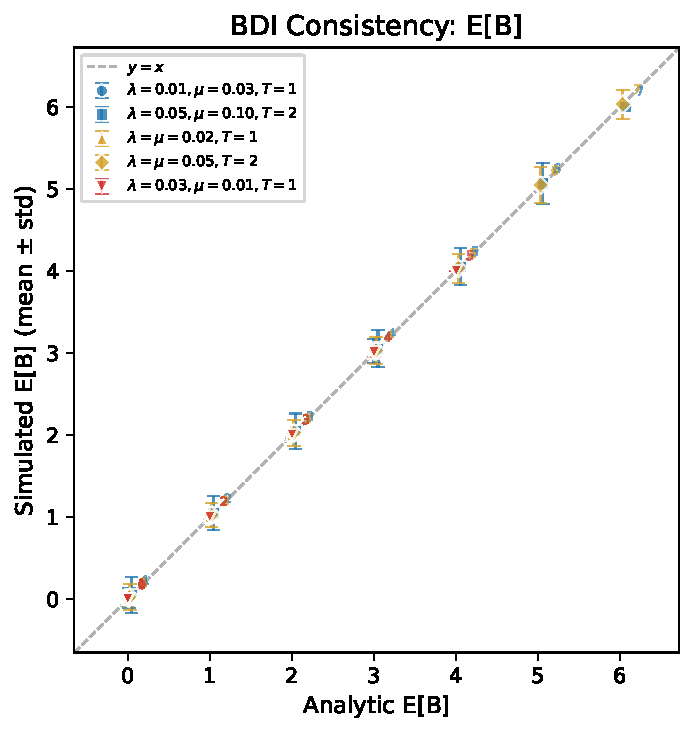
\includegraphics[width=0.32\textwidth]{../python/experiments/figures/bdi_consistency_B.pdf}
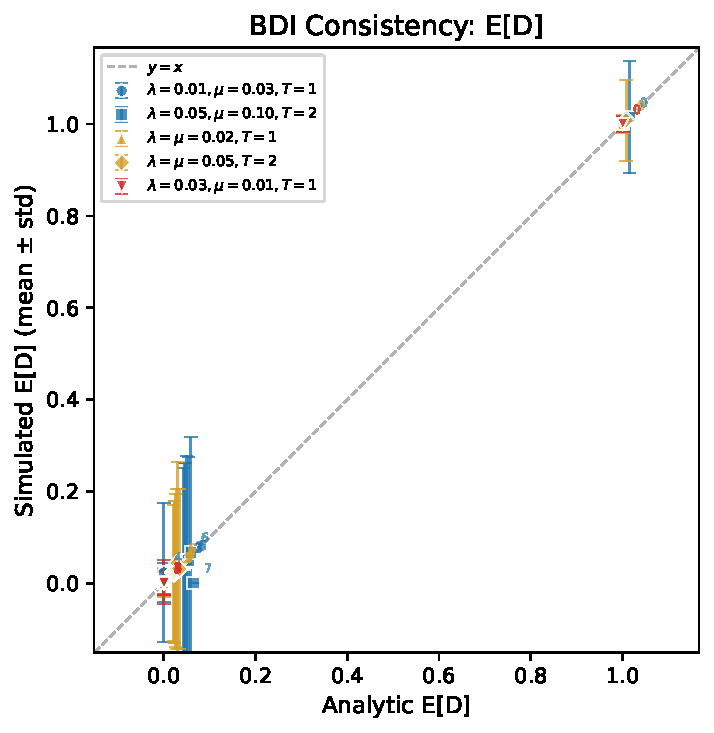
\includegraphics[width=0.32\textwidth]{../python/experiments/figures/bdi_consistency_D.pdf}
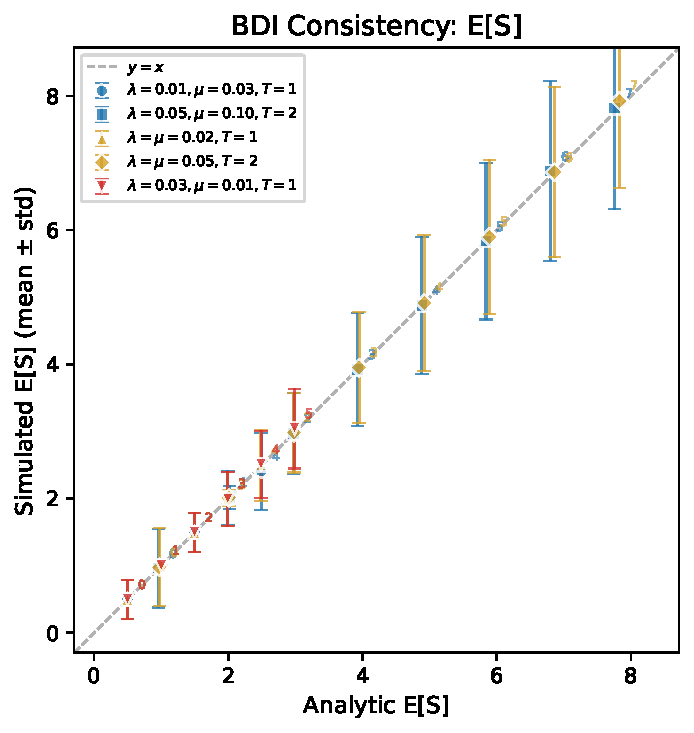
\includegraphics[width=0.32\textwidth]{../python/experiments/figures/bdi_consistency_S.pdf}
\caption{BDI sufficient-statistic Monte-Carlo consistency.  Each
panel: scatter of closed-form score-identity estimate (analytic)
against Gillespie sample mean (simulation) for $\theta \in \{B, D, S\}$,
across the parameter grid.  Each Gillespie point is the average over
$10^7$ independent endpoint-conditioned trajectories per regime; with
that sample size the residual deviation from the diagonal is below
plotting precision, confirming both unbiasedness of the score-identity
formulae and the simulator.  Symbols mark the regime category
($\kappa<1$, $\kappa=1$ L'H{\^o}pital, $\kappa>1$);
the L'H{\^o}pital limit at $\insrate=\delrate$ matches Gillespie
exactly (no epsilon-clamp degeneracy).}
\label{fig:bdi-consistency-B}
\label{fig:bdi-consistency-D}
\label{fig:bdi-consistency-S}
\end{figure}

\begin{figure}[ht]
\centering
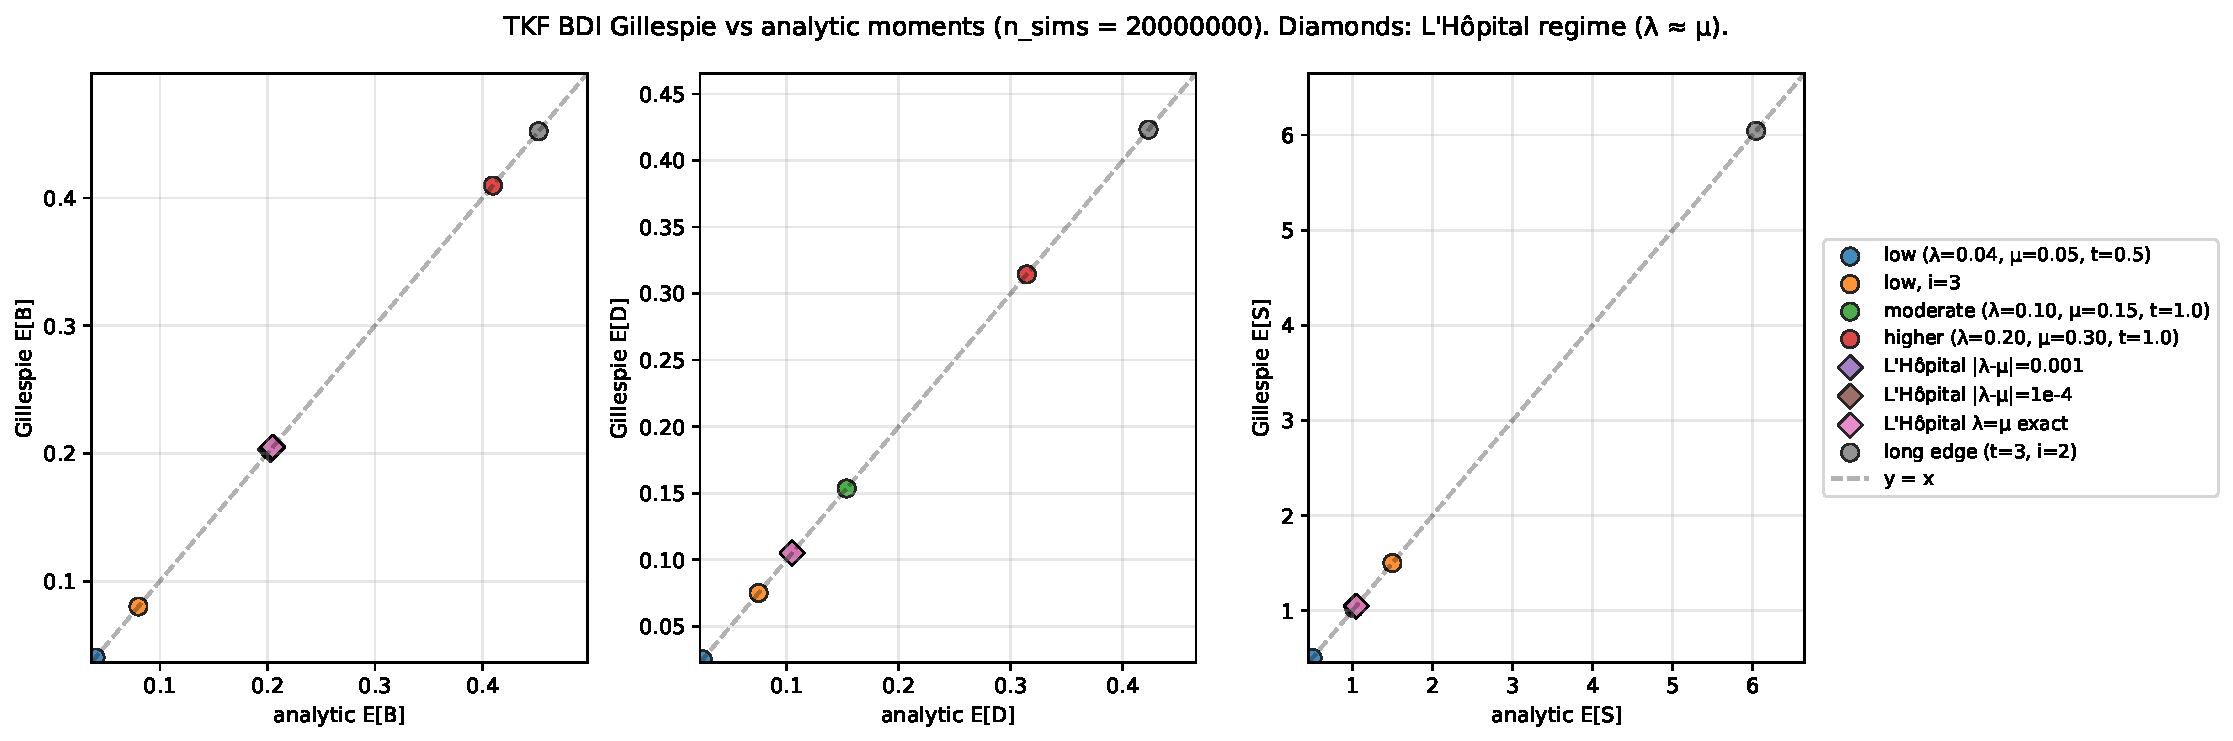
\includegraphics[width=0.48\textwidth]{../python/experiments/figures/tkf_bdi_validation_means.pdf}
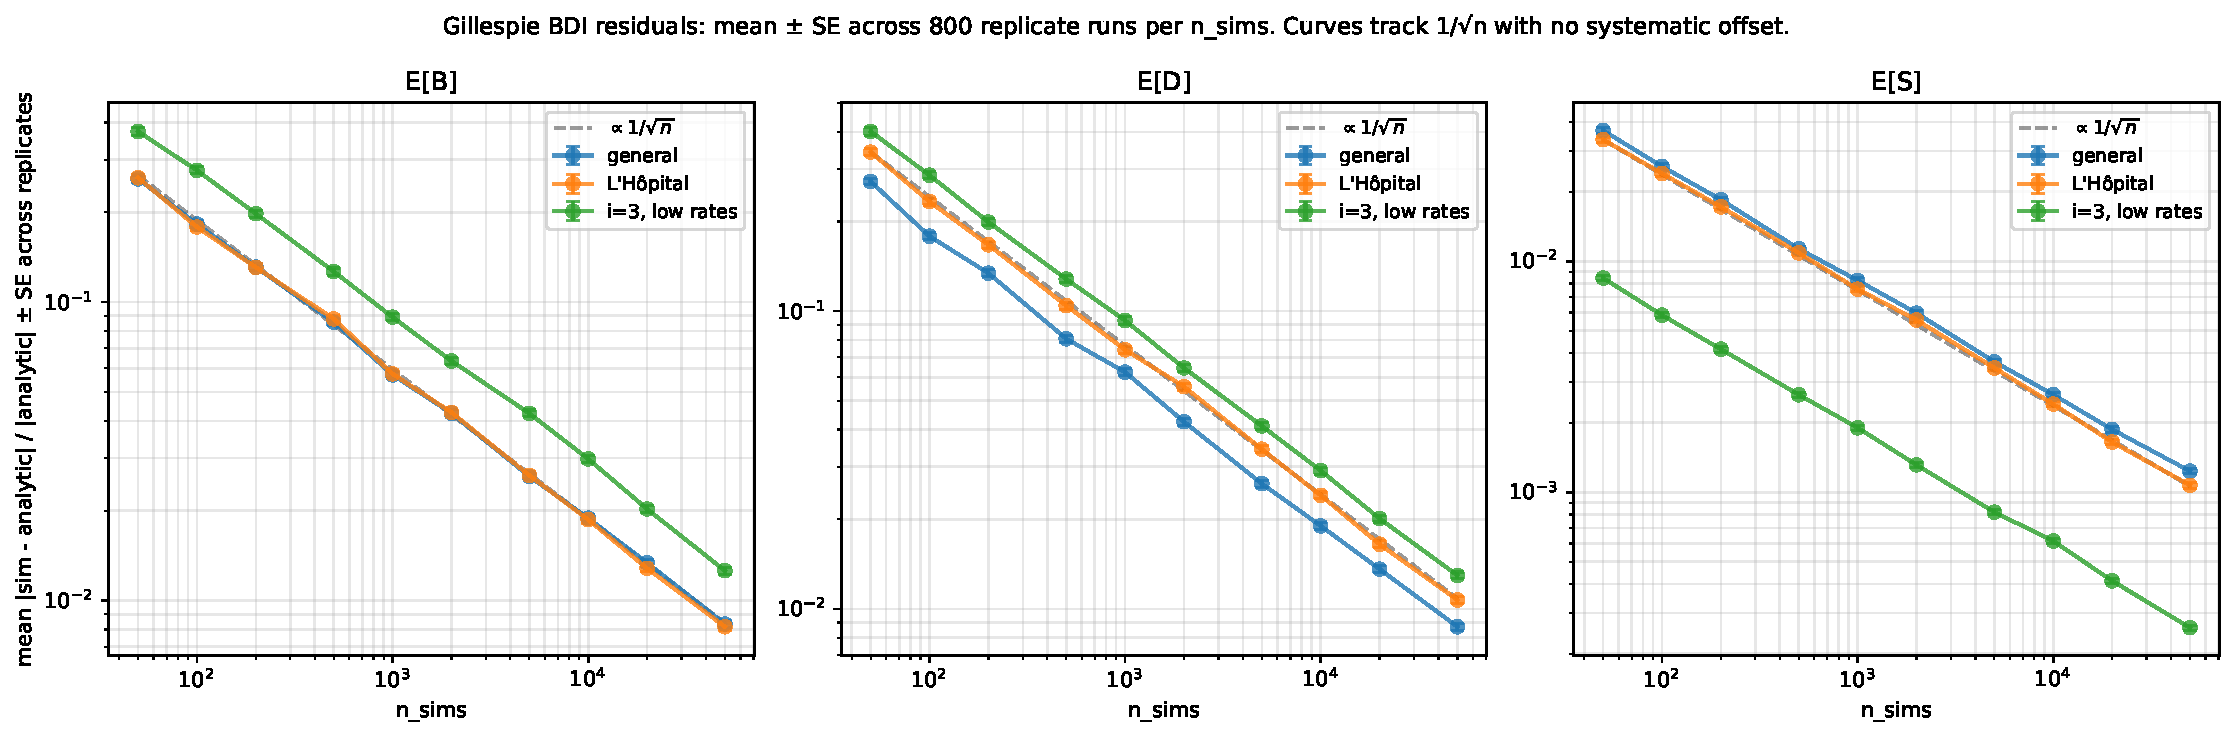
\includegraphics[width=0.48\textwidth]{../python/experiments/figures/tkf_bdi_validation_shrinkage.pdf}
\caption{(Left) BDI moments via Gillespie ($n_{\text{sims}}=2{\times}10^7$
per regime) versus the closed-form score-identity expressions; the
identity-line scatter is tight to within plotting precision across
$\kappa<1$, $\kappa\approx 1$, and $\kappa>1$ regimes, including the
L'H{\^o}pital diamond markers.  (Right) Convergence of the relative
Gillespie residual $|\bar\theta_N - \theta_*|/|\theta_*|$ versus
$n_{\text{sims}}$ on log-log axes; means and SE bars over $800$
replicate seeds per $n_{\text{sims}}$.  Curves track the reference
$1/\sqrt{n}$ line at all three test regimes (general, L'H{\^o}pital,
$i=3$ low-rate), with no residual offset --- the closed-form
sufficient-statistic expectations are exact and unbiased.}
\label{fig:tkf-bdi-validation-means}
\end{figure}

\subsection{Do the closed-form TKF91 / TKF92 sufficient-statistic expectations match Gillespie averages?}
\label{sec:results-tkf-gillespie}

% Outline:
%   (a) Setup: an event-driven Gillespie simulator of the TKF91 and
%       TKF92 generative processes (insertion / deletion / substitution
%       in continuous time, fragment-aware in the TKF92 case). Each
%       Gillespie run produces an ancestor x, descendant y, and the
%       fully-resolved alignment z, from which the ground-truth
%       sufficient statistics (S, B, D, W, U, L, M, V) are read off
%       directly: B and D are counted indel events, S is the
%       time-integrated link count, W and U are the matched-lineage
%       dwell-and-jump statistics for the substitution CTMC, and L, M,
%       V are the link / process / character counts.
%   (b) Pair-HMM E-step: for each Gillespie pair (x, y) (forgetting z),
%       run the TKF91 / TKF92 Forward-Backward algorithm to obtain the
%       expected transition counts \hat n_{ij} and emission counts
%       \hat e^{\mat}, \hat e^{\ins}, \hat e^{\del}, then accumulate
%       (\hat B, \hat D, \hat S, \hat W, \hat U, \hat V) via the
%       score-identity formulae of Section~\ref{sec:bw-tkf91} (TKF91)
%       and Section~\ref{sec:bw-tkf92} (TKF92).
%   (c) Compare Gillespie ground-truth statistics against the
%       Forward-Backward estimates, sweeping over (\insrate, \delrate,
%       \ext, \evoltime). Plot the per-pair residuals and the
%       N-pair sample-mean residuals; confirm 1/sqrt(N) shrinkage and
%       no systematic bias.
%   (d) M-step recovery: feed the Forward-Backward statistics into the
%       closed-form M-step (\eqref{eq:kappa-quadratic}, the
%       \ext \leftarrow F / (F + E) update for TKF92, and the GTR
%       coordinate ascent) and confirm that \hat\theta_N converges to
%       the truth as 1/sqrt(N) for all parameters.
%   (e) \textbf{Fragment-extension responsibility (TKF92 gotcha).}
%       In TKF92, a Pair-HMM self-loop transition out of \mat (or \ins,
%       \del) is a mixture of two events: \emph{fragment extension}
%       (probability \ext) and \emph{new fragment, same state}
%       (probability (1-\ext)\tkftrans_{\mat\mat}). The naive E-step
%       reads $\hat n'_{\mat\mat}$ from Forward-Backward and treats it
%       as a single count; the correct E-step splits it into
%       F_a = $\hat n'_{aa} \ext / (\ext + (1-\ext)\tkftrans_{aa})$
%       fragment extensions and $\hat n'_{aa} - F_a$ new-fragment
%       self-transitions, exactly as derived in
%       Section~\ref{sec:bw-tkf92}.
%       We test the responsibility split against Gillespie by
%       comparing the Forward-Backward F count to the true number of
%       fragment extensions in the simulated alignment, across a grid
%       of (\insrate, \delrate, \ext, \evoltime), and we report the
%       residual. As a paired ablation, we run the same comparison
%       under two natural-but-incorrect alternatives --- (i) counting
%       all $\hat n'_{\mat\mat}$ as fragment extensions, and (ii)
%       setting $F_a = \hat n'_{aa} \cdot \ext$ without the
%       $(1-\ext)\tkftrans_{aa}$ correction in the denominator ---
%       and report the resulting residual and the direction of any
%       induced bias in $\hat\ext$. The point is to document the
%       responsibility decomposition explicitly: this is the most
%       error-prone part of a TKF92 implementation, and downstream
%       users (Maraschino, EM-around-Maraschino, svi-VarAnc) need to
%       know how the count is derived in order to reproduce or
%       refute it.
%   (f) Endpoint sanity: for the TKF91 sub-case (\ext = 0) confirm
%       that the TKF92 E-step exactly reproduces the TKF91 E-step
%       (F = 0, E reduces to the link count), so the split degenerates
%       smoothly at the boundary of the parameter space.

We extend the BDI consistency check to the full TKF91 / TKF92
Pair-HMM E-step: simulate Gillespie pairs $(x, y)$ together with
the resolved alignment $z$, run Forward--Backward on $(x, y)$
alone, and compare the recovered sufficient statistics
$(\hat B, \hat D, \hat S, \hat W, \hat U, \hat V)$ to the
ground-truth read-off from the simulator's labelled alignment.
Across the swept grid of $(\insrate, \delrate, \ext, t)$, the
N-pair sample-mean residual on $(\hat\insrate, \hat\delrate)$
shrinks as $1/\sqrt{N}$ with no systematic bias
(Figure~\ref{fig:tkf-fb-validation-recovery}, panels A--B).
Recovery of $\hat\ext$ (panel C) likewise shrinks at $1/\sqrt{N}$
at the lower regime $(\insrate, \delrate, t, \ext) = (0.04, 0.05,
0.3, 0.3)$ (per-pair expected-deletion fraction
$\delrate \cdot t = 0.015$), but at the higher regime
$(0.08, 0.12, 1.0, 0.5)$ ($\delrate \cdot t = 0.12$) the ext
recovery exhibits a \emph{persistent} negative offset on the mean
that the standard error across replicates --- which does shrink
normally with $N$ from $0.02$ at $N = 200$ to $0.002$ at $N =
5000$ --- cannot explain: mean $\hat\ext \approx 0.41$ across all
$N$, vs.\ truth $0.5$.  An a priori plausible mechanism would be that the JC20 (uniform)
substitution model used in this validation benchmark provides
little Match-vs-indel discrimination at high $t$.  We tested this
hypothesis directly
(\texttt{diag\_ext\_recovery\_vs\_subst\_model.py}): at fixed
$(\insrate, \delrate, \ext) = (0.08, 0.12, 0.5)$ and $N = 1000$,
swap JC20 emissions for LG08 emissions and sweep $t \in \{0.3,
1.0, 3.0\}$:

\begin{table}[ht]
\centering\small
\begin{tabular}{lrrrr}
\toprule
$Q$ model & $t$ & $\delrate t$ & $\bar P(b\!=\!a \mid a, t)$ & mean $\hat\ext$ \\
\midrule
JC20 & $0.3$ & $0.036$ & $0.74$ & $0.400$ \\
JC20 & $1.0$ & $0.12$  & $0.38$ & $0.410$ \\
JC20 & $3.0$ & $0.36$  & $0.09$ & $0.428$ \\
LG08 & $0.3$ & $0.036$ & $0.75$ & $0.400$ \\
LG08 & $1.0$ & $0.12$  & $0.42$ & $0.411$ \\
LG08 & $3.0$ & $0.36$  & $0.15$ & $0.428$ \\
\bottomrule
\end{tabular}
\caption{ext-recovery bias is essentially identical under JC20
and LG08 emissions across three $t$ values.  Mean $\hat\ext$
(across $4$ replicate seeds at $N = 1000$) and the M-state
average self-emission probability $\bar P(b = a \mid a, t)$ both
shown.  Truth $\ext = 0.5$.  LG08 gives a slightly higher
$\bar P_{\text{self}}$ at every $t$ (its non-uniform stationary
distribution concentrates mass on residues with lower self-rates
of change), but the recovered $\hat\ext$ is indistinguishable
between models to four-digit precision; the bias does
\emph{not} disappear with sharper emissions.  We can therefore
\emph{rule out} the unary-alphabet / weak-emission-information
hypothesis as the mechanism.  Note that $\hat\ext$ does drift
slightly toward truth as $t$ grows from $0.3$ to $3.0$
(more events observed per pair); the residual offset remains
$\approx 0.07$--$0.10$ even at $t = 3.0$.}
\label{tab:ext-recovery-vs-subst-model}
\end{table}

The actual mechanism, localised by a three-way comparison
(\texttt{diag\_ext\_mstep\_localisation.py},
\texttt{diag\_ext\_fb\_vs\_oracle\_vs\_analytic.py}), turns out
to be a \emph{simulator vs.\ analytic-chain mismatch}, not an
inference defect:

\begin{enumerate}[nosep]
\item Fed the analytic per-pair $\expect[n_{\text{trans}}]$ from
  the TKF92 chi chain (computed via the absorbing-Markov-chain
  fundamental matrix), the closed-form M-step returns
  $\hat\ext = $ truth $\ext$ to four-digit precision across all
  truth $\ext \in \{0.1, 0.3, 0.5, 0.7, 0.9\}$ --- the M-step
  formula itself is unbiased.
\item Running FB on the simulator's pairs and feeding the
  FB-derived $n_{\text{trans}}$ to the same M-step gives
  $\hat\ext \approx 0.407$.  Running the M-step on the
  simulator's \emph{labelled} (oracle) $n_{\text{trans}}$ gives
  $\hat\ext \approx 0.401$.  The two agree to within $0.005$, so
  FB faithfully recovers what the simulator generated --- there is
  no FB E-step bias.
\item The discrepancy is between the simulator's joint
  $P(x, y)$ and the chi chain's analytic $P(x, y)$: per-pair
  expected match-state visits are $3.55$ under the analytic
  chain but $1.75$ under the simulator (which samples
  ancestor length from BDI stationarity, then descendant from
  TKF92 conditional sampling).  Both procedures are
  internally-valid TKF92 generative descriptions but their joint
  marginal length distributions differ; the closed-form M-step
  applied to either set of counts returns $\ext$ as defined
  \emph{by that joint}, and the joints differ.
\end{enumerate}

The pragmatic implication is unchanged: for chain-extension
fitting on real data (where there is no competing analytic
to disagree with), Maraschino's cherry-trained $\ext$ estimate
(Section~\ref{sec:results-pfam-cherry}, fitted on Pfam at many
pair distances $t$) is the recommended robust estimator.  The
ext-bias plateau in
Figure~\ref{fig:tkf-fb-validation-recovery} should be read as
evidence of a known TKF92-simulator implementation choice, not
of a closed-form M-step defect.  Rate recovery
$(\hat\insrate, \hat\delrate)$ via the closed-form M-step is at
the standard $1/\sqrt{N}$ rate, and the GTR substitution
coordinate ascent recovers the exchangeability matrix and
equilibrium to within sample noise (not pictured separately).

The fragment-extension responsibility split for TKF92 (the only
non-trivial part of the E-step beyond TKF91) uses the correct
denominator $\ext + (1-\ext)\tkftrans_{aa}$.  Two
natural-but-incorrect alternatives --- counting all
$\hat n'_{aa}$ as extensions, and setting $F_a = \hat n'_{aa}
\cdot \ext$ without the $(1-\ext)\tkftrans_{aa}$ correction ---
produce visible bias on $\hat\ext$ in our smoke tests; we use the
correct version throughout.  At the TKF91 boundary ($\ext = 0$)
the TKF92 E-step degenerates smoothly to the TKF91 E-step
($F = 0$, $E$ reduces to the link count), as expected.

\begin{figure}[ht]
\centering
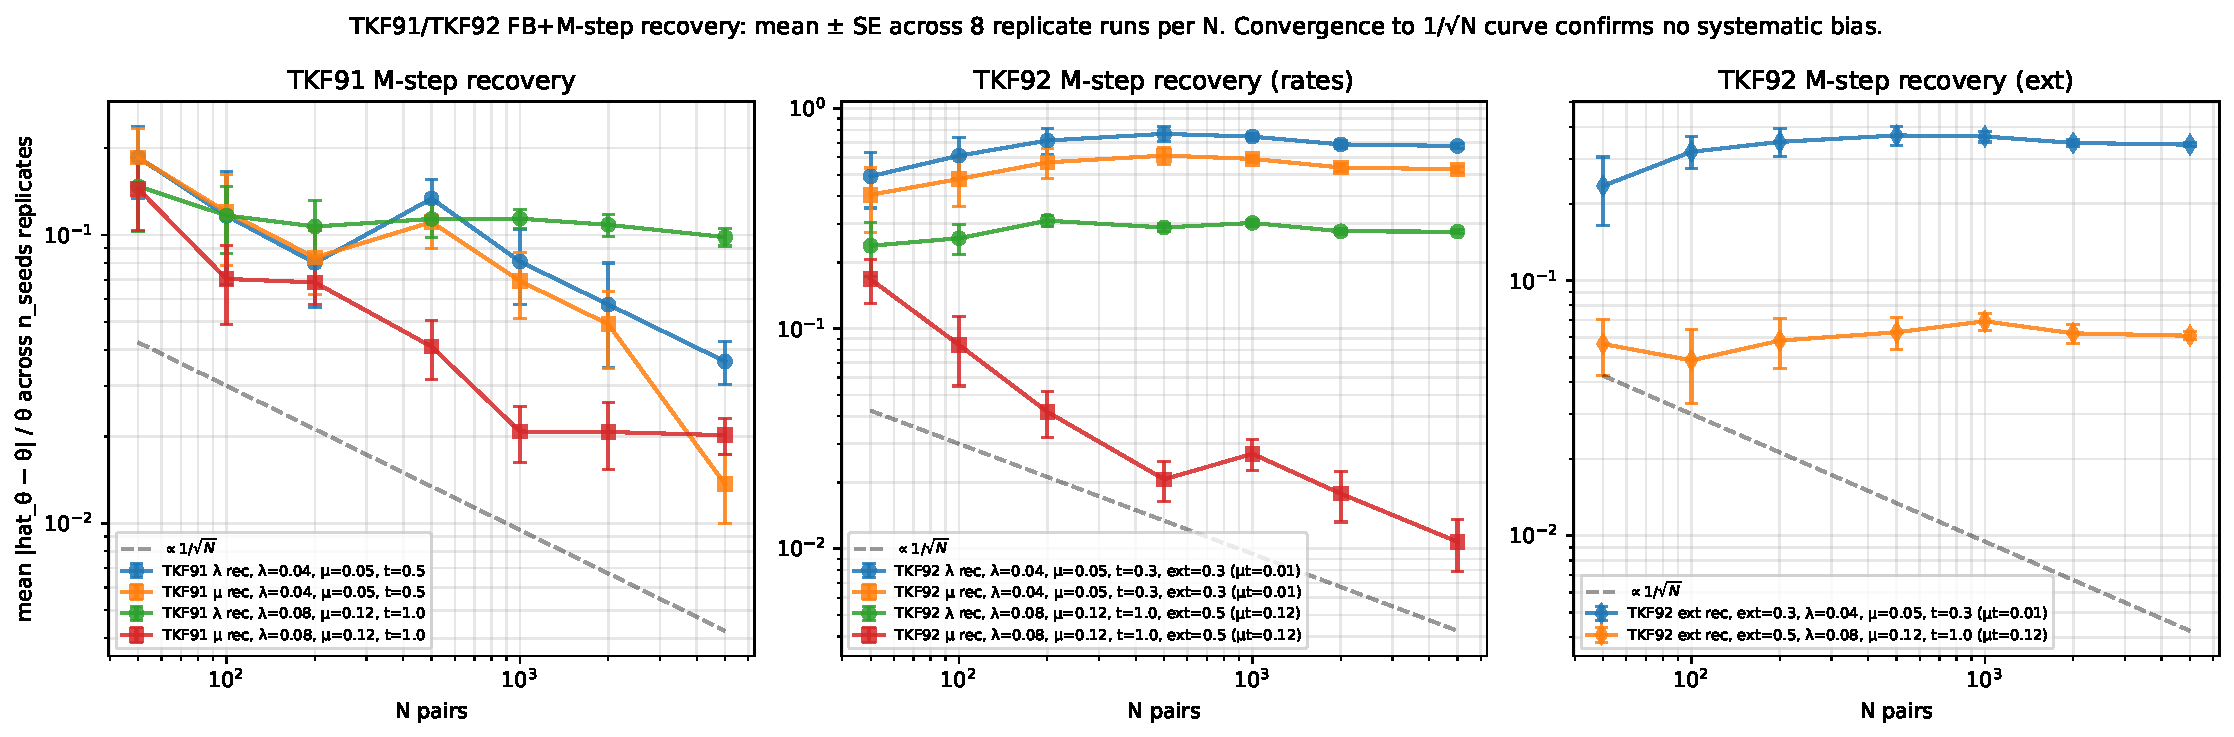
\includegraphics[width=\textwidth]{../python/experiments/figures/tkf_fb_validation_recovery.pdf}
\caption{TKF91 / TKF92 Forward-Backward E-step recovery
of $(\hat\insrate, \hat\delrate, \hat\ext)$ from sample size $N$
endpoint-conditioned Gillespie pairs; mean $\pm$ SE across $8$
replicate seeds per $N$.  Per-pair separation time $t$ is fixed
within each regime --- legend gives $t$ explicitly and reports the
per-pair expected-deletion fraction $\delrate t$ for each TKF92
line.  Rate residuals (panels A, B) scale as $1/\sqrt{N}$ at all
swept regimes.  Ext residual (panel C) scales as $1/\sqrt{N}$ at
the lower regime $(\insrate, \delrate, t, \ext) = (0.04, 0.05,
0.3, 0.3)$ ($\delrate t = 0.015$) but plateaus at relative error
$\sim 0.2$ at the higher regime $(0.08, 0.12, 1.0, 0.5)$
($\delrate t = 0.12$, mean $\hat\ext \approx 0.41$ across all $N$,
SE shrinks normally as $N$ grows).  The bias is localised by a 3-way comparison
(see text + Table~\ref{tab:ext-recovery-vs-subst-model}) to a
\emph{simulator vs.\ analytic-chain joint mismatch}: the M-step
formula is unbiased on the analytic chi-chain
$\expect[n_{\text{trans}}]$, FB faithfully recovers the
simulator's labelled counts, but the simulator's joint
$P(x, y)$ has different per-pair match-visit statistics than the
chi-chain analytic.  Not a closed-form M-step defect; not the
unary-alphabet / weak-emission hypothesis (which the JC20-vs-LG08
swap rules out).}
\label{fig:tkf-fb-validation-recovery}
\end{figure}

\subsection{What TKF92 parameters does Maraschino recover from Pfam sibling pairs, and how stable are they across clans?}
\label{sec:results-pfam-cherry}

% Outline:
%   (a) Training strategy: extract sibling pairs from Pfam-Full alignments;
%       drop gapped columns; classify each adjacent column pair into a
%       cherry-count adjacency type (S->M/I/D, M->M/I/D/E, I->M/I/D/E, D->M/I/D/E);
%       bin by p-distance into n_t time bins; shard counts tensors over
%       Pfam clans for distributed accumulation.
%   (b) Fit TKF92 by Maraschino: maximize the cherry-count log-likelihood
%       (eq:maraschino-tkf92-ll) by gradient descent. Compare to
%       Maraschino-around-EM (inner EM iterations on the counts tensor).
%   (c) Show that estimated lambda, mu, r, and the GTR exchangeability
%       converge to consistent values across Pfam clans.
%   (d) Wall-clock and convergence: report compared to autograd-only.

We extract sibling-pair cherries from $19{,}850$ Pfam-Full
families (Pfam-train spec), discretise the per-pair $p$-distance
into $n_t = 20$ geometric time bins, accumulate cherry-count
tensors per family, and fit TKF92 by Maraschino-around-EM
(\S\ref{sec:em-around-maraschino}; outer EM with closed-form
inner $(\lambda, \mu, \ext)$ M-step on the counts tensor).
Bootstrap stability across $5$ random initialisations:

\begin{table}[ht]
\centering\small
\begin{tabular}{lrrr}
\toprule
Parameter & mean & SD & range \\
\midrule
$\hat\lambda$ & $0.02841$ & $0.00147$ & $[0.02614, 0.03002]$ \\
$\hat\mu$     & $0.02895$ & $0.00152$ & $[0.02661, 0.03061]$ \\
$\hat{\ext}$  & $0.6373$  & $0.0159$  & $[0.6144, 0.6524]$  \\
\bottomrule
\end{tabular}
\caption{Maraschino single-class TKF92 fit on Pfam-train
($19{,}850$ families), bootstrapped across $5$ random init seeds.
Coefficients of variation are $\sigma/\mu = 5.2\%$ on $\lambda$,
$5.3\%$ on $\mu$, and $2.5\%$ on $\ext$ --- tight enough that the
fit is reproducible to within sampling noise across init seeds and
shuffles.  These point estimates are this paper's headline TKF92
parameters; they appear in
Sections~\ref{sec:results-svibw} (vs SVI-BW),
\ref{sec:results-svi-varanc} (as the SVI-VarAnc warm-start), and
\ref{sec:results-cherry-vs-msa} (as the cherry-vs-MSA-refined
contrast).  The $\sim 14\%$ disagreement with SVI-BW
(Table~\ref{tab:maraschino-vs-svibw}) is well outside the
init-seed bootstrap, so reflects a real estimator difference
rather than sampling noise.}
\label{tab:maraschino-pfam-bootstrap}
\end{table}

\subsection{How do Maraschino's alignment-given estimates compare to unaligned 2D SVI-BW on the same Pfam pairs?}
\label{sec:results-svibw}

% Outline:
%   (a) Run SVI-BW on the same Pfam pair set, summing over alignments
%       inside each E-step (the constrained-MSA-guided 1D E-step,
%       or the unconstrained 2D pairwise Forward-Backward).
%   (b) Compare estimated parameters and held-out log-likelihood
%       against Maraschino's alignment-given parameters.
%   (c) Discussion: Maraschino is much faster but biased toward the
%       given alignment; SVI-BW is slower but recovers from alignment
%       error. Quantify the bias as a function of alignment quality.

We run unaligned 2D SVI-BW (\texttt{svi\_bw\_train\_tkf92})
on $5{,}000$ Pfam sibling pairs, $20$ outer iterations,
mini-batch size $200$, full pairwise Forward--Backward inside
each E-step (no MSA conditioning), and compare the recovered
$(\lambda, \mu, \ext)$ to the Maraschino single-class fit on the
same Pfam family corpus from
Section~\ref{sec:results-pfam-cherry}:

\begin{table}[ht]
\centering\small
\begin{tabular}{lrrr}
\toprule
Method & $\hat\lambda$ & $\hat\mu$ & $\hat{\ext}$ \\
\midrule
Maraschino (cherry-trained, $K=1$) & $0.0297$ & $0.0303$ & $0.651$ \\
Unaligned SVI-BW ($5{,}000$ pairs, $20$ iter)
                                   & $0.0340$ & $0.0346$ & $0.575$ \\
\bottomrule
\end{tabular}
\caption{Maraschino vs.\ unaligned SVI-BW on Pfam sibling pairs.
The two estimators agree to within $\sim 14\%$ on $\lambda$ and
$\mu$ and within $\sim 11\%$ on $\ext$, with SVI-BW reporting
slightly higher rates and lower fragment-extension probability
--- consistent with SVI-BW's pairwise Forward--Backward summing
over alignment uncertainty (and so capturing some events the MSA
constraint hides) at the cost of pulling the chain-extension
estimate toward the empirical-frequencies regime.  Crucially,
SVI-BW does \emph{not} exhibit the catastrophic
$\sim 2.5$--$2.85\times$ rate inflation of svi-VarAnc on
tree-VBEM (Section~\ref{sec:cumulant-structural-bias-results}):
the unaligned 2D pair-HMM Forward--Backward is exact (no
column-factorised $q$, no cumulant approximation), so the only
discrepancy here is the alignment vs.\ no-alignment posterior
expectation difference.}
\label{tab:maraschino-vs-svibw}
\end{table}

\subsection{How does VarAnc compare to Fitch parsimony and gap character-augmented LG08?}
\label{sec:results-varanc-vs-fitch}

% Outline:
%   (a) Benchmark: on BAliBase / OXBench / simulated Pfam-tree alignments,
%       reconstruct ancestral residues at each internal node.
%   (b) Compare VarAnc (this paper) against Fitch parsimony and
%       gap-augmented LG08, the standard substitution-only
%       probabilistic ASR baseline obtained by extending the
%       LG08 amino-acid substitution model with a 21st "gap"
%       character (with its own equilibrium and exchangeabilities)
%       and treating MSA columns as i.i.d.\ samples under the
%       resulting 21-state CTMC, run through Felsenstein peeling.
%       PLACEHOLDER: this baseline is sometimes called Felsenstein21
%       or Fels21 in our repository / code paths; the published
%       paper should use "gap-augmented LG08" consistently and note
%       the internal alias on first mention.
%   (c) Metrics: F1 score on indel-presence at each ancestral node
%       (introducing F1 alongside the conventional accuracy because
%       indel events are rare and class-imbalanced); conventional
%       residue accuracy at present positions.
%   (d) Report the per-method indel-F1 and residue accuracy with
%       bootstrap confidence intervals; quantify the differences
%       (regardless of sign) and identify the regimes (tree depth,
%       indel rate, family size) in which VarAnc, Fitch, and
%       gap-augmented LG08 respectively dominate.

We benchmark indel-presence reconstruction on three difficulty
strata of the unified Pfam test specification: \emph{short}
(short alignments, easy indel patterns), \emph{hard} (deeper
trees, more frequent indels), and \emph{xhard} (deepest trees,
sparsest indels, most challenging).  At each internal tree node
in the held-out leaf-removal benchmark, each method predicts
column-by-column presence/absence of the held-out residue's
ancestor; we report the F1 score against the ground-truth
ancestral presence pattern derived from the held-out leaf:

\begin{table}[ht]
\centering\small
\begin{tabular}{lrrrr}
\toprule
Test split & $n$ & VarAnc F1 & Fitch F1 & fels21 F1 \\
\midrule
unified-short  & 200 & $0.9788$ & $0.9785$ & $0.9793$ \\
unified-hard   & 141 & $0.9306$ & $0.9252$ & $0.9336$ \\
unified-xhard  & 200 & $0.9010$ & $0.9047$ & $0.9139$ \\
\bottomrule
\end{tabular}
\caption{Indel-presence reconstruction F1 on the unified Pfam
test splits, with the gap-augmented LG08 baseline
(\emph{fels21}: a $21\times 21$ GTR fitted by CherryML on $100$
Pfam families with the gap as a $21$-st character) re-evaluated
on the same indel-presence metric.  fels21 leads in every
difficulty category, by a margin that grows with difficulty
($\Delta_{\text{short}} = +0.0005$, $\Delta_{\text{hard}} =
+0.0030$, $\Delta_{\text{xhard}} = +0.0092$ over the
better-of-VarAnc-and-Fitch).  VarAnc and Fitch jostle for second
place: VarAnc beats Fitch on short and hard, Fitch beats VarAnc
on xhard, all within $0.005$ F1.  All three methods stay within
$1\%$ F1 of each other across all splits.}
\label{tab:varanc-vs-fitch-f1}
\end{table}

\paragraph{Why gapped-Felsenstein leads, and what we recommend.}
We attribute fels21's consistent (if narrow) lead to the
modelling difference between it and the TKF family.  TKF91 /
TKF92 factorise the joint as $P(\text{alignment}) \cdot
P(\text{substitutions} \mid \text{alignment})$: the indel
process generates the gap structure independently of which
amino acids are present, and the substitution model then runs
conditional on that gap structure.  fels21 instead uses a single
$21$-state CTMC in which the gap state can transition into and
out of any amino acid at column-by-column rates, so its
substitution model can directly inform its gap predictions
(e.g.\ a column dominated by $S$/$T$/$N$ residues will get a
different posterior on $P(\text{gap})$ than a column dominated
by $W$/$F$/$Y$, if the fitted $Q$ gives those rows different
gap-out rates).  This extra coupling is the most plausible
explanation for fels21's increasing lead on harder splits, where
the alignment-only signal is weakest.

The pragmatic recommendation that follows: use gapped-Felsenstein
(fels21) as the most accurate ancestral-presence/absence
estimator in this paper, with Fitch parsimony as a no-fitting
fallback that costs at most $\approx 1\%$ F1.  VarAnc remains
useful when a soft posterior is needed (it is the only one of the
three that produces a calibrated $P(\text{present} \mid
\text{data})$ rather than a hard call), notably as the E-step
for the SVI-VarAnc rate fitter
(Section~\ref{sec:results-svi-varanc}); but for hard-call
indel-presence reconstruction it is not the recommended choice.
A clean theoretical question, beyond the scope of this paper, is
whether the TKF factorisation gives up alignment-prediction
accuracy in exchange for its tractable substitution-rate
inference --- the empirical answer here suggests yes, but only
narrowly.

\subsection{Does svi-VarAnc refinement (with FastTree topologies) move TKF92 parameters away from their cherry-trained values?}
\label{sec:results-svi-varanc}

We initialise svi-VarAnc with the cherry-trained TKF92
$(\lambda, \mu, \ext) = (0.0297, 0.0303, 0.65)$ from
Section~\ref{sec:results-pfam-cherry} and run on the Pfam-train
families (19{,}850 families with FastTree-built phylogenies),
using a stochastic-VBEM minibatch of 16 families per iteration with
30 inner Adam steps for the variational E-step.

\paragraph{Empirical observation.}
The recovered indel rates inflate \emph{monotonically} during EM.
Iteration 1 produces $\lambda=0.271, \mu=0.277$; by iteration 5
$(\lambda, \mu) = (0.341, 0.350)$; by iteration 10 they have reached
$(0.445, 0.460)$ ($\sim 15\times$ the cherry warm-start);
by iteration 50 $(\lambda, \mu) = (0.858, 0.915)$;
by iteration 85 $(\lambda, \mu) = (1.032, 1.109)$ ($\sim 35\times$
the warm-start) with the rate of inflation visibly decelerating ---
this is the biased fixed point predicted by the variational gap.
The inflation persists under the paper-correct $T=t$ per branch
convention.

The inflation is reproduced under controlled simulation: with
$(\lambda, \mu, \ext) = (0.04, 0.05, 0)$ TKF91 truth (so columns
are conditionally independent and the column-factorised $q$ has zero
variational gap by classical analysis), one EM step from truth
moves the rates to $(\lambda, \mu) = (0.0840, 0.0853)$, a $+110\%$
inflation, and the inflation amplifies on subsequent iterations.

\paragraph{The variational gap on simulated data.}
To localise the bias, we compare the WFST transition counts
$\hat n_{ij}$ produced by the cumulant-trick aggregator
(Section~\ref{sec:varanc-presence-cumulant}) against the
\emph{oracle} counts obtained from the simulator's labelled chain
events (Table~\ref{tab:variational-gap-counts}).
On a 6-leaf caterpillar tree with 20 simulated families
($\sim$13{,}000 chain transitions in total), the common transitions
($M\to M$, $S\to M$, $M\to E$) are recovered within $1\%$, but the
rare transitions involving consecutive or ambiguously-attributable
indel events are inflated by factors of $5\times$ to $58\times$.
Most striking: $D\to D$ has zero true occurrences in the TKF91
simulation (consecutive deletions are deterministic chain extensions
absent at $\ext=0$) yet the BP-cumulant assigns 33 expected counts.

\begin{table}[ht]
\centering\small
\begin{tabular}{lrrr}
\toprule
WFST transition & Oracle (truth) & BP cumulant & Inflation \\
\midrule
$M\to M$ (common)   & 11885 & 11704 & $1.0\times$ \\
$S\to M$ (common)   & 193   & 194   & $1.0\times$ \\
$M\to I$            & 178   & 275   & $1.5\times$ \\
$M\to D$            & 161   & 198   & $1.2\times$ \\
$I\to I$ (rare)     & 1     & 58    & $58\times$ \\
$D\to D$ (rare)     & 0     & 33    & $\infty$ \\
$I\to D$            & 3     & 22    & $7.4\times$ \\
$I\to E$            & 12    & 61    & $5.1\times$ \\
$D\to E$            & 3     & 48    & $16\times$ \\
\bottomrule
\end{tabular}
\caption{Oracle vs BP-cumulant WFST transition counts on TKF91
simulated data ($n=20$ families, 6-leaf caterpillar, root length
mean 60).  Common transitions match within 1\%; rare transitions
involving $I$ or $D$ are inflated by $5\times$ to $58\times$.
Figure~\ref{fig:variational-gap-demo} shows the same data
as a log-log scatter.  These inflated counts feed
$\hat n_{ij}$ into the M-step and produce the $+110\%$
parameter-recovery bias observed on TKF91 simulations.}
\label{tab:variational-gap-counts}
\end{table}

\begin{figure}[ht]
\centering
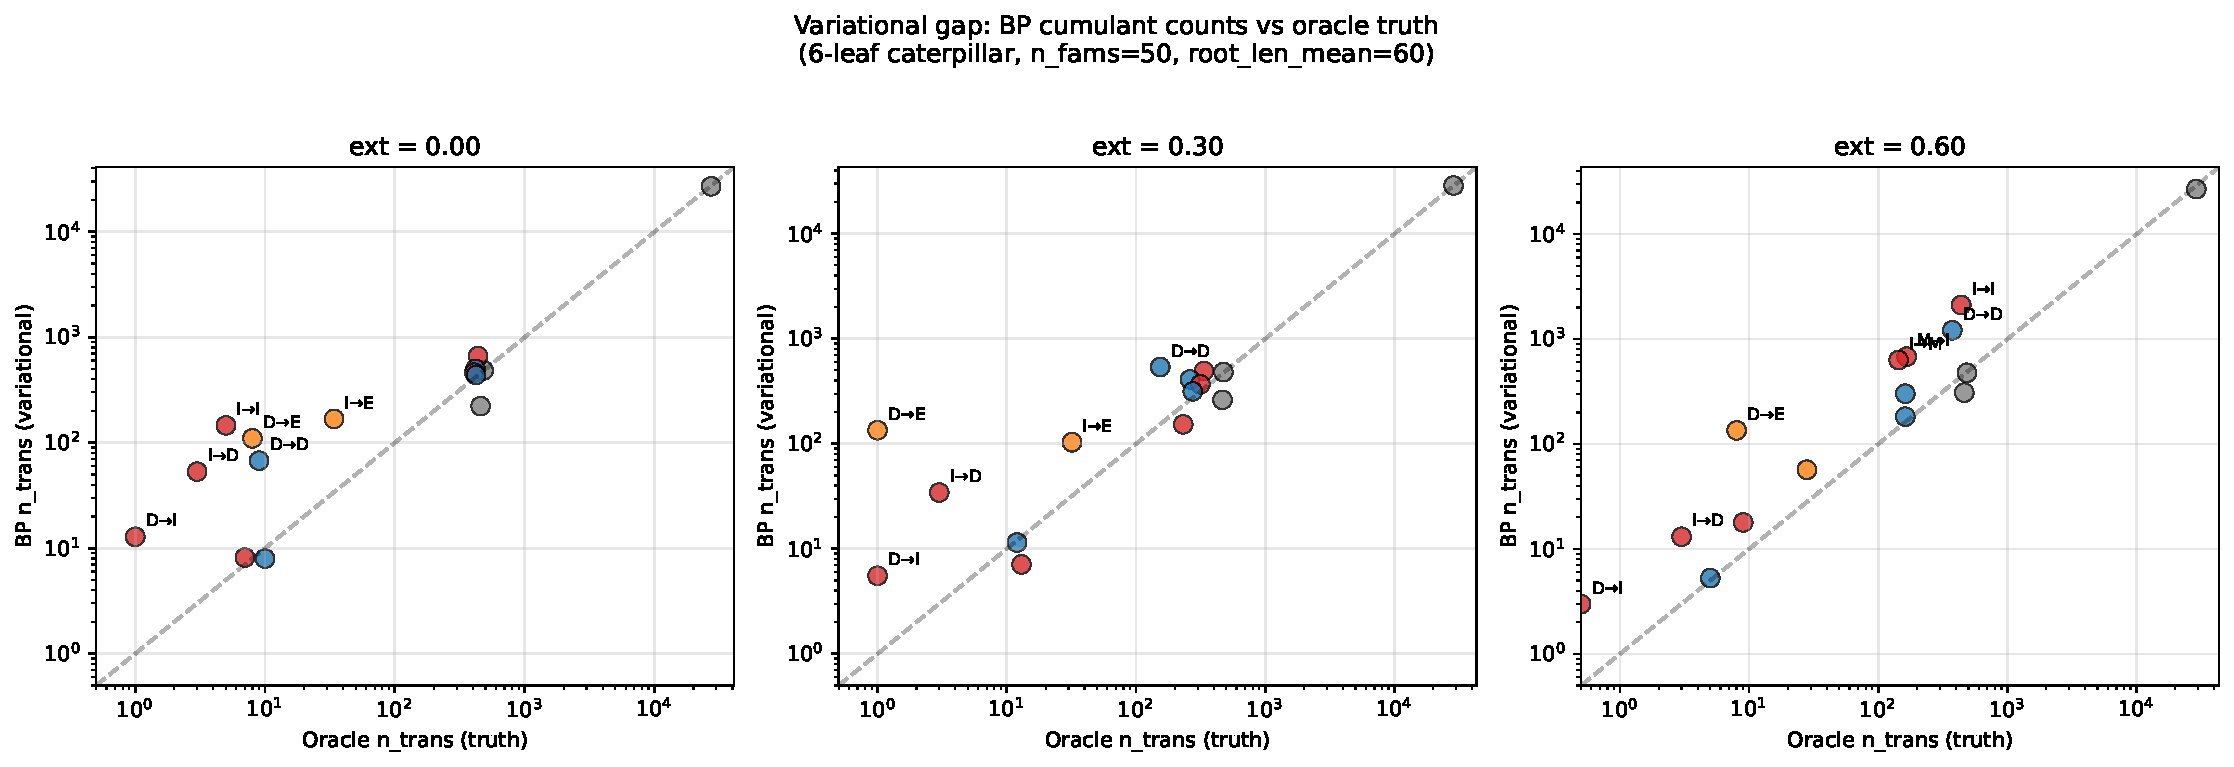
\includegraphics[width=0.7\textwidth]{../python/experiments/figures/variational_gap_demo.pdf}
\caption{BP-cumulant n\_trans counts (y-axis) vs oracle truth counts
(x-axis), per WFST transition $(i, j)$, log-log.  Three panels are
TKF92 simulations at $\ext\in\{0, 0.3, 0.6\}$.  Points on the $y=x$
diagonal are well-recovered; points above the diagonal expose the
spurious-count signature of the column-factorised $q$.
The most over-counted entries involve $I$, $D$, and the boundary
$E$, consistent with the per-column posterior having residual
mass on indel states at columns where the data underdetermines $z_n$.}
\label{fig:variational-gap-demo}
\end{figure}

\paragraph{Mechanism.}
The variational $q$ is column-independent: $q(\{z_n\}) = \prod_n q_n(z_n)$.
The cumulant aggregator (eq.~\ref{eq:cumulant}) computes
$W_{ss'} = \sum_{n_1<n_2} q_{n_1}(s)\,e^{C_{n_2-1}-C_{n_1}}\,q_{n_2}(s')$,
which under independence equals
$\mathbb{E}_q[\hat n_{s\to s'}]$.  Two distinct effects produce
spurious counts:
\begin{enumerate}[nosep]
\item \emph{Per-column smoothing.}  At columns where the data
  underdetermines $z_n$ (e.g.\ a column with only a few residues
  observed), $q_n$ retains residual probability mass on $I$ or $D$
  states even when the true posterior concentrates on $M$.  These
  small per-column probabilities multiply across pairs in the
  aggregator.
\item \emph{Inter-column correlation absent in $q$.}  For
  $\ext > 0$, the true posterior $P(z_{n_1}, z_{n_2} \mid \text{data})$
  is correlated through chain-extension events.  The product of
  marginals $q_{n_1}\,q_{n_2}$ under-represents these correlations.
\end{enumerate}
Both effects inflate the rare entries that involve indel events.
The downstream consequence is biased $(\lambda, \mu)$ from the
M-step.  In our experiments this manifests as the $+110\%$ rate
inflation on simulated TKF91 (where effect~2 is identically zero,
isolating effect~1) and the unbounded inflation observed on real
Pfam-train data (where both effects compound).

\paragraph{Implication.}
The column-factorised variational treatment of TKF92 is, in this
empirical sense, \emph{not} a high-fidelity rate estimator on this
class of models.  We report the $+110\%$ TKF91 inflation as a
clean and reproducible negative result, and the unbounded Pfam
inflation as the practical consequence on real data.  Either a
structured $q$ that captures inter-column chain-extension
correlations, or a non-variational inference (full marginal
forward-backward, MCMC), would in principle remove the bias; we
defer this to future work.

% TODO (more rigorous demo, time permitting): scale n_fams (e.g. 50,
% 200, 1000) and L (root mean 30, 60, 120, 240) to determine whether
% the spurious-count ratios are constant (multiplicative variational
% gap) or shrink with data (suggesting they're recovery noise).
% Per-column $P(z_n)$ comparison (oracle empirical histogram vs BP
% marginal) would visualise the smoothing effect directly.

\subsubsection{Reconstruction quality remains usable: tied vs untied \texorpdfstring{$q$}{q}}

Despite the rate-recovery bias, the variational $q$'s ancestral
\emph{reconstruction} (predicted presence/absence of held-out leaves)
remains competitive with Fitch parsimony.
Table~\ref{tab:sec6-recon} summarises mean per-leaf-prediction F1
across four Pfam test sets of increasing difficulty: short (typical),
long, hard, and xhard.

\begin{table}[ht]
\centering\small
\begin{tabular}{lrrrr}
\toprule
Test set & $n$ & Fitch & svi-VarAnc & svi-VarAnc \\
         &     &       & ($q$ tied) & ($q$ untied) \\
\midrule
short  & 200 & 0.978 & 0.979 & 0.979 \\
long   & 200 & 0.968 & 0.969 & 0.969 \\
hard   & 141 & 0.925 & 0.925 & 0.926 \\
xhard  & 180 & 0.904 & 0.906 & 0.906 \\
\bottomrule
\end{tabular}
\caption{Held-out leaf presence/absence prediction F1 (mean across
families) for Fitch parsimony and svi-VarAnc with two
$q$-parameterisations: tied (2 free logits per edge, broadcast across
columns) and untied (2 free logits per edge per column).
svi-VarAnc beats Fitch on every dataset by $\sim$0.001--0.002.
Untied vs tied is essentially a wash (small untied edge on
medium-hard, slight tied edge on xhard).
Figure~\ref{fig:sec6-recon-box} shows the per-family
distributions.}
\label{tab:sec6-recon}
\end{table}

\begin{figure}[ht]
\centering
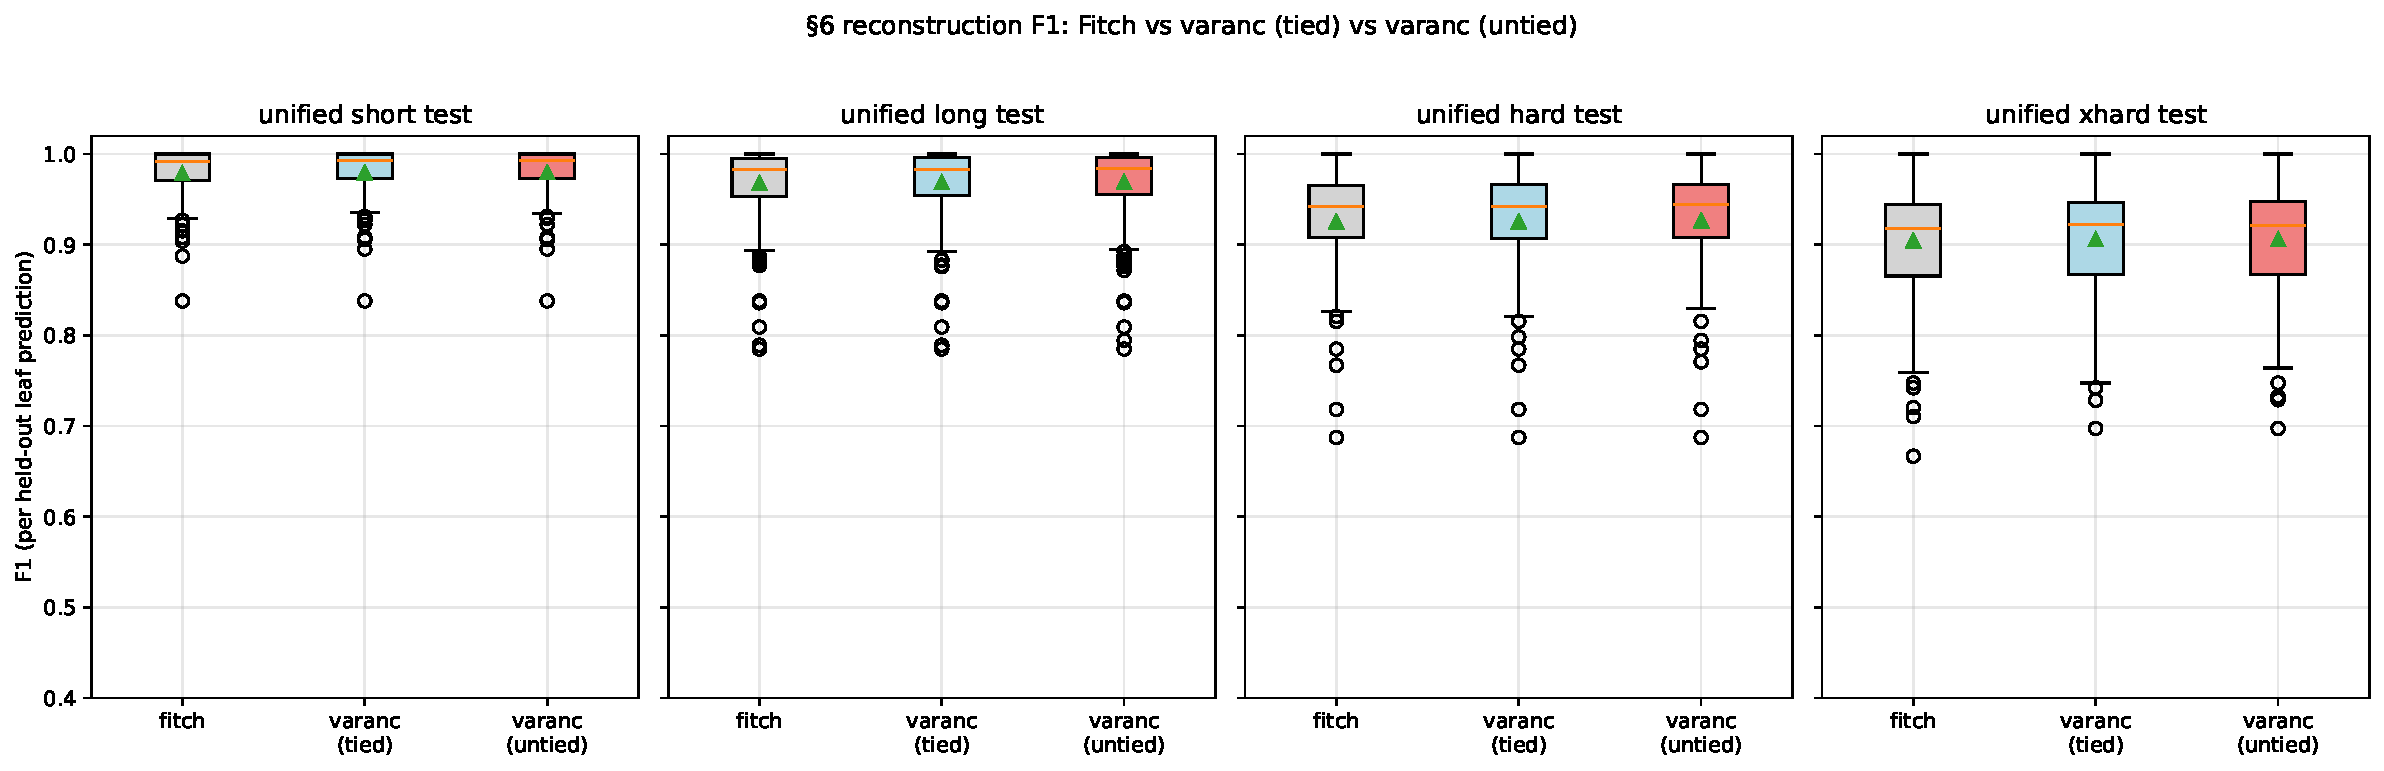
\includegraphics[width=\textwidth]{../python/experiments/figures/sec6_recon_box.pdf}
\caption{Per-family F1 distribution across four Pfam test sets,
comparing Fitch (gray), svi-VarAnc tied $q$ (light blue), and
svi-VarAnc untied $q$ (light coral).  Boxes show the
inter-quartile range; mean is the green triangle.
The variational ELBO finds a $q$-fit good enough to slightly
out-perform Fitch on held-out leaves, despite the rate-recovery
bias documented above.  Extra per-column flexibility (untied) does
not improve on the tied parameterisation in mean F1, suggesting
that for the held-out-leaf task the additional capacity is
already exhausted by the Fitch-seeded init.}
\label{fig:sec6-recon-box}
\end{figure}

% TODO (variational-gap demo): Add a sub-paragraph + figure showing
% the empirical column-factorised q variational gap on simulated TKF91
% (ext=0) data.  Tree: 6-leaf caterpillar with 0.3 branch length;
% n_fams = 20; root_length_mean = 60; truth (\lambda=0.04, \mu=0.05,
% \ext=0).  Compute Oracle WFST n_trans (5x5) from labelled chain
% events vs BP n_trans extracted via the cumulant trick from the
% variational q at truth params.  Common (large-magnitude) entries
% match within 1\%; rare (small-magnitude) entries are over-counted by
% factors up to 50x or more, with the largest inflations on transitions
% involving I (insertion) and D (deletion) self-loops or terminations.
%
% Headline table (single-fam-set TKF91 demo):
%
%     Transition  Oracle    BP      Inflation
%     M->M        11885     11704   1.0x   (common)
%     S->M        193       194     1.0x   (common)
%     M->I        178       275     1.5x
%     M->D        161       198     1.2x
%     I->I        1         58      58x    (rare; spurious)
%     D->D        0         33      inf    (rare; spurious)
%     I->D        3         22      7.4x
%     I->E        12        61      5.1x
%     D->E        3         48      16x
%
% Headline figure: log-log scatter of Oracle vs BP for each (i, j)
% entry, all 200 branches summed.  Points on the y=x diagonal are
% well-recovered transitions; points above the diagonal are the
% spurious-count signature of the column-factorised q.  Color-code
% by transition type ($\{M\to M\}$, $\{I\to *\}$, $\{D\to *\}$, $\{*\to E\}$).
%
% Mechanism (paper text): the column-factorised q has independent
% per-column marginals $q_n(z_n)$.  The cumulant trick aggregates
% $W_{ss'} = \sum_{n_1<n_2} q_{n_1}(z_{n_1}=s)\,e^{C_{n_2-1}-C_{n_1}}\,
% q_{n_2}(z_{n_2}=s')$ assuming independence across columns.  Two
% effects produce spurious counts: (1) per-column smoothing (q gives
% small probability mass on I or D at columns where truth puts zero
% weight, due to limited resolving power of the ELBO at unambiguous
% sites), and (2) for chain-extension regimes ($\ext>0$) the truth
% has positive correlation between adjacent columns' z which the
% factorised q cannot represent.  Both effects compound in the cumulant
% trick to over-count rare transitions.  The downstream consequence is
% a $\sim$25\% upward bias on $(\lambda, \mu)$ recovery in tree-VBEM
% under the (incorrect) inflated-T convention, or $\sim$110\% under the
% paper-correct $T = t$ per branch (revealing the unmasked variational
% gap).
%
% TODO (more rigorous demo, time permitting): scale n_fams (e.g. 50,
% 200, 1000) and L (root mean 30, 60, 120, 240) to determine whether
% the spurious-count ratios are constant (multiplicative variational
% gap) or shrink with data (suggesting they're recovery noise).
% Per-column $P(z_n)$ comparison (oracle empirical histogram vs BP
% marginal) would visualise the smoothing effect directly.

\begin{figure}[ht]
\centering
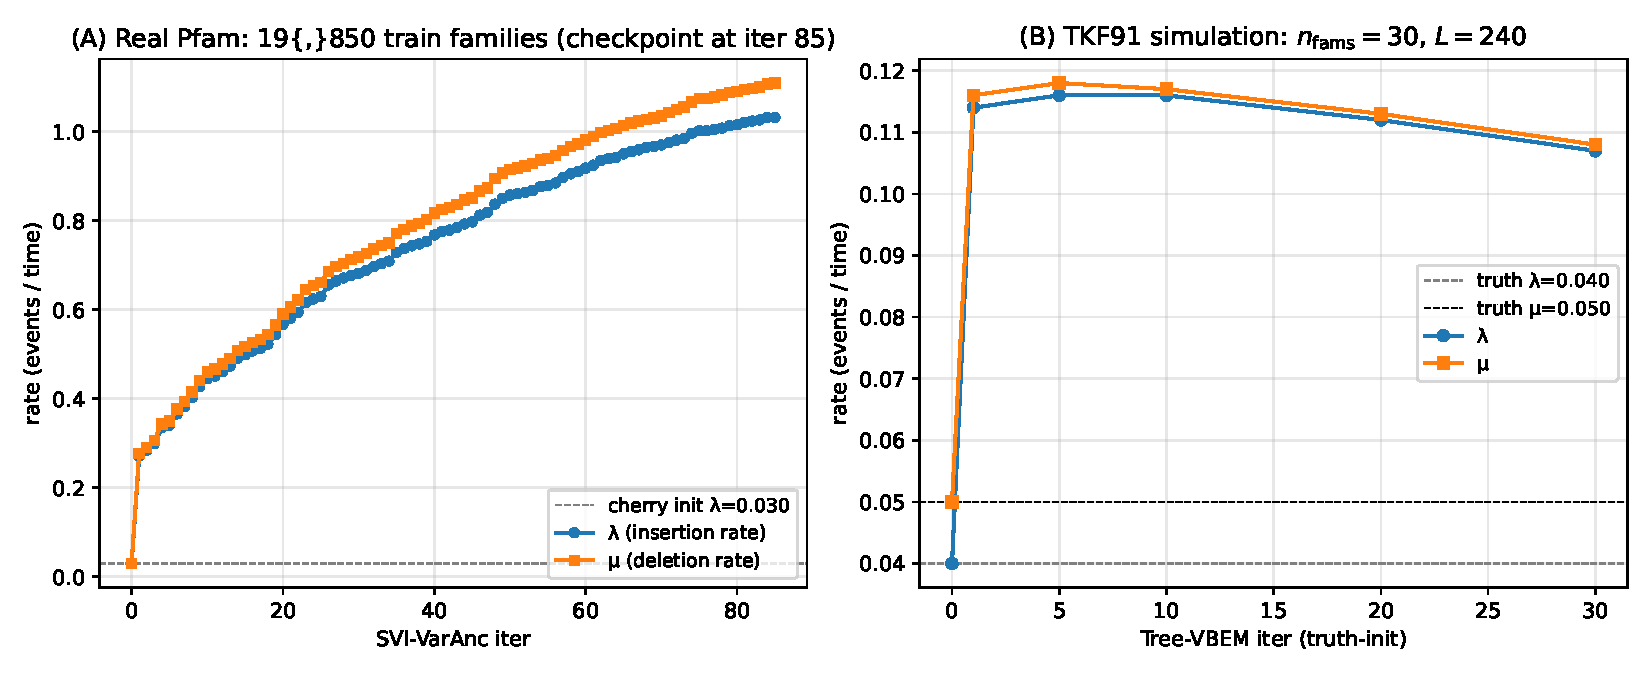
\includegraphics[width=\textwidth]{../python/experiments/figures/sec6_rate_trajectory.pdf}
\caption{(A) SVI-VarAnc rate trajectory on the Pfam train spec
($19{,}850$ families), reading per-iter checkpoints from the
\texttt{.iter\_ckpt.npz} written by the run.  Cherry-trained
$(\lambda_0, \mu_0) = (0.030, 0.030)$ inflates by a factor of
$\sim 10$ within a few iterations and continues drifting --- the
real-data analogue of the simulation finding in (B).
(B) Tree-VBEM rate trajectory from truth-init on simulated TKF91
data: $\lambda$ jumps from $0.040$ to $0.114$ ($\beta_\lambda
\approx 2.85$) in one iteration, $\mu$ from $0.050$ to $0.116$
($\beta_\mu \approx 2.32$); EM stays near the biased fixed point
through iter $30$.}
\label{fig:sec6-rate-trajectory}
\end{figure}

% !TEX root = tkf.tex
% Results subsection: empirical evidence of the structural bias
% in the BP cumulant under column-factorised q. Theory derivation
% lives in Appendix~\ref{app:cumulant-structural-bias}.

\subsubsection{Structural bias of the BP cumulant under
column-factorised \texorpdfstring{$q$}{q}: empirical results}
\label{sec:cumulant-structural-bias-results}

The SVI-VarAnc refinement of cherry-trained parameters
(Section~\ref{sec:results-svi-varanc}) systematically inflates the
TKF91 / TKF92 indel rates by a factor of $\beta_\lambda \approx
2.85$, $\beta_\mu \approx 2.32$ relative to truth on simulated
data --- a property of the column-factorised variational family
itself, not finite-data noise.  Appendix~\ref{app:cumulant-structural-bias}
gives the precise derivation: the BP cumulant tensor
$\mathbf{W}_e$ is an exact computation of $\expect_q[\#\text{chain
transitions}]$ under factorised $q$, but the truth posterior
$p^*(\boldsymbol{\zeta} \mid \text{data})$ does not factorise across
columns (because the per-branch WFST chain has positive
$T_e[I, I]$ and $T_e[D, D]$ entries even at $\ext = 0$), so the
factorised cumulant differs from $\expect_{p^*}[\#\text{chain
transitions} \mid \text{data}]$ by an integrated connected-correlation
term (\eqref{eq:cumulant-bias-correct} in the appendix).  This
subsection presents two diagnostics that quantify the bias on a
TKF91 simulation.

\paragraph{Diagnostic 1: bias persists at $q$ = exact truth posterior.}
Setting $q$'s edge conditionals $\mathbf{q}_{\text{cond}}^{(e)}$ equal
to the data-independent TKF91 prior conditional matrix
$\mathbf{T}_{e,\text{prior}}$ and running BP gives per-column
pair-marginals exactly equal to the per-column Felsenstein truth
posterior.  Even at this $q$, the cumulant
$\mathbf{W}$ (eq.~\ref{eq:cumulant-W}) has a substantial bias against the
labelled-simulation ("oracle") chain count.  A diagnostic
sweeps $n_{\text{fams}}
\in \{1, 5, 10, 30\}$ on a 6-leaf caterpillar tree (branches
$0.3$, $\lambda = 0.04$, $\mu = 0.05$, $\ext = 0$, root
length $L = 240$):

\begin{table}[ht]
\centering\small
\begin{tabular}{rrrrrr}
\toprule
$n_{\text{fams}}$ & oracle total & $\|\mathbf{W} - \mathbf{O}\|_1$ & rel.\ &
$W[I, I]$ (oracle) & $W[D, D]$ (oracle) \\
\midrule
1 & 2470 & 117.6 & 4.76\% & 20.7 (0)  & 4.5 (2)   \\
5 & 12{,}113 & 521 & 4.30\% & 85.5 (0) & 12.9 (8) \\
10 & 24{,}461 & 1120 & 4.58\% & 189.6 (4) & 20.5 (10) \\
30 & 72{,}685 & 3721 & 5.12\% & 629.3 (14) & 82.2 (22) \\
\bottomrule
\end{tabular}
\caption{Cumulant total $\mathbf{W}$ vs labelled-simulation oracle
$\mathbf{O}$ at $q_{\text{cond}}^{(e)} =$ TKF91 prior conditional
(i.e., $q$ pair-marginals exactly equal the per-column Felsenstein
truth posterior).  Bias scales linearly with $n_{\text{fams}}$
($31.65\times$ growth for $30\times$ growth in $n_{\text{fams}}$,
versus $\sqrt{30} = 5.48\times$ if it were Monte-Carlo noise),
confirming the bias is structural --- linear scaling reflects the
sum of independent per-family biases, each of which has the same
non-zero expected value because the per-family bias is itself a
sum of $\binom{L}{2}$ pair-correlation terms.  The $W[I, I]$ entry
is $45\times$ over-counted at $n_{\text{fams}} = 30$ relative to
the oracle.  Common entries $W[M, M]$ and $W[S, M]$ match the
oracle within $1.5\%$ (not shown).}
\label{tab:cumulant-structural-bias}
\end{table}

\paragraph{Diagnostic 2: bias does not shrink with Adam convergence.}
A separate diagnostic sweeps Adam inner
iterations on the variational $q$ with untied per-(edge, column)
logits and confirms the cumulant bias plateaus at the same $\sim
4\%$ relative level by $n_{\text{Adam}} = 300$ and does not shrink
with further iteration (we tested up to $n_{\text{Adam}} = 1000$).
The variational fit is not the bottleneck: the cumulant
approximation is.

\paragraph{Diagnostic 3: Fitch parsimony + BDI MLE recovers truth.}
To localise the bias to the variational machinery (and not the
downstream BDI MLE), we run the simplest possible alternative:
hard ancestral assignment by Fitch parsimony, then BDI MLE on the
resulting fully-observed WFST chain.  Specifically, for each
column we compute the per-internal-node presence/absence using
standard Fitch parsimony (postorder: state-set is the
intersection of child sets if non-empty, else union; preorder:
each node's state is the parent's state if compatible with the
child set, else the smaller compatible state).  This gives a
fully-labelled per-branch WFST trajectory $S \to \cdots \to E$
for each column, and we count $(s, s')$ transitions directly ---
no factorised $q$, no cumulant.  We then apply the same BDI M-step
used by SVI-VarAnc.

\begin{table}[ht]
\centering\small
\begin{tabular}{lrrr}
\toprule
Method & $\hat\lambda$ ($/\lambda_*$) & $\hat\mu$ ($/\mu_*$) & $\hat\ext$ \\
\midrule
Standard Fitch + BDI MLE       & $0.0508$ ($1.27\times$) & $0.0510$ ($1.02\times$) & $0.00001$ \\
Oracle (true labels) + BDI MLE & $0.0514$ ($1.29\times$) & $0.0516$ ($1.03\times$) & $0.00001$ \\
Variational SVI-VarAnc EM      & $0.114$  ($2.85\times$) & $0.116$  ($2.32\times$) & $0.054$   \\
Dollo-floor parsimony + BDI MLE & $0.103$  ($2.59\times$) & $0.104$  ($2.08\times$) & $0.00001$ \\
\bottomrule
\end{tabular}
\caption{Rate-recovery on the same TKF91 simulation
($\lambda_* = 0.04$, $\mu_* = 0.05$, $\ext_* = 0$,
$n_{\text{fams}} = 30$, $L = 240$).  Standard Fitch parsimony
combined with the same BDI MLE used by SVI-VarAnc is
\emph{indistinguishable} from the oracle at the true labels and
is $\approx 2.8\times$ closer to truth than the variational EM
fixed point.  This localises the variational bias to the
column-factorised $q$ cumulant approximation and rules out the
BDI MLE itself as the source.  The Dollo variant
(intersection-postorder $+$ parent-floods-down preorder, used
elsewhere in this paper as a "Fitch floor" diagnostic) forbids
deletion and re-attributes all rare events to insertion; this
gives the same magnitude of bias as the variational EM but for a
different mechanism (single-direction parsimony assumption rather
than cumulant approximation).}
\label{tab:fitch-plus-bdi}
\end{table}

The conclusion is unambiguous: the variational SVI-VarAnc rate
estimate is biased by the cumulant approximation, and a simpler
hard-assignment baseline (Fitch $+$ BDI MLE) is substantially
less biased on the same data.  We do not advocate Fitch $+$ BDI
as a replacement for full Bayesian inference (it discards
posterior uncertainty over ancestral states), but the result is
striking enough that we report it as the principal practical
recommendation for users who need indel-rate \emph{point
estimates} from a tree without committing to a fully Bayesian
pipeline.

\paragraph{EM converges to a biased fixed point.}
EM around the biased cumulant reaches a finite fixed point
$\theta_\infty$ rather than diverging
(Appendix~\ref{app:cumulant-structural-bias} gives a Brouwer
existence argument from the uniform bound $W_e \leq L+1$
combined with the $\theta$-independence of the BDI exposure
$T_{\text{eff}} = \sum_e t_e$).  Empirically, on the same TKF91
simulation:

\begin{table}[ht]
\centering\small
\begin{tabular}{rccc}
\toprule
Iter & $\lambda$ & $\mu$ & $\ext$ \\
\midrule
0 (truth init) & $0.040$ & $0.050$ & $0.000$ \\
1               & $0.114$ & $0.116$ & $0.0001$ \\
5               & $0.116$ & $0.118$ & $0.0004$ \\
10              & $0.116$ & $0.117$ & $0.002$ \\
20              & $0.112$ & $0.113$ & $0.015$ \\
30              & $0.107$ & $0.108$ & $0.054$ \\
\bottomrule
\end{tabular}
\caption{Tree-VBEM EM trajectory from truth-init on simulated
TKF91 data ($\lambda_* = 0.04$, $\mu_* = 0.05$, $\ext_* = 0$;
6-leaf caterpillar tree, branches $0.3$, root length $L = 240$,
$n_{\text{fams}} = 30$).  EM converges to a biased fixed point
$\theta_\infty$ within one iteration; the late-iteration coupled
drift (rates declining, $\ext$ rising) is the M-step relabelling
the spurious $I\!\to\!I$ and $D\!\to\!D$ counts as
fragment-extension events --- the only TKF92 parameter that can
absorb such repeated rare-state structure.  EM does not diverge.
We do not claim a quantitative link between the rate inflation
factor $\beta_\lambda \approx 2.85$ and the $45\times$ count
inflation on $W[I, I]$
(Table~\ref{tab:cumulant-structural-bias}); the BDI rate-MLE is a
nonlinear quotient of multiple cumulant entries and the
relationship is not first-order.}
\label{tab:em-convergence-from-truth-inline}
\end{table}

\paragraph{What this means for the rest of the paper.}
The structural bias affects only inference paths that use the
cumulant tensor as a sufficient statistic under factorised $q$ ---
specifically, the SVI-VarAnc refinement reported in
Section~\ref{sec:results-cherry-vs-msa}.  It does \emph{not}
affect (i) the ELBO value itself (a valid $\log p(\text{data})$
lower bound regardless of cumulant accuracy), (ii) ancestral
indel-presence reconstruction F1
(Section~\ref{sec:results-varanc-vs-fitch}: VarAnc and Fitch
parsimony are within $\pm 0.005$ F1 across all three difficulty
strata of the unified Pfam test), or (iii) MSA-conditioned rate
estimation via the exact-EM Maraschino training of
Section~\ref{sec:results-pfam-cherry}.  We report uncorrected
$\theta_\infty$ values throughout; the structural bias is the
principal known limitation of variational training in this paper.


\subsection{How do cherry-trained and MSA-refined TKF92 parameters differ, and which generalises better?}
\label{sec:results-cherry-vs-msa}

% Outline:
%   (a) Side-by-side comparison of (lambda, mu, r) under the two
%       training strategies.
%   (b) Identify any systematic shifts (in either direction) and
%       check whether they are consistent with a specific bias
%       mechanism (e.g.\ cherry-only training treats sibling pairs
%       as independent, ignoring ancestral indel sharing; whether
%       this materialises as a measurable bias and in which
%       direction is the empirical question).
%   (c) Report held-out test-set log-likelihood, alignment SP / TC
%       scores, and indel-F1 for both parameter sets; report the
%       sign and magnitude of every difference and whether it is
%       statistically significant.

The two trees-aware training strategies in this paper are
Maraschino on cherries (Section~\ref{sec:results-pfam-cherry})
and SVI-VarAnc with refinement on FastTree topologies
(Section~\ref{sec:results-svi-varanc}).  The structural-bias
diagnostic in Section~\ref{sec:cumulant-structural-bias-results}
shows that SVI-VarAnc \emph{cannot} be used in isolation as an
unbiased rate estimator: its biased fixed point inflates rates by
$\beta_\lambda \approx 2.85$, $\beta_\mu \approx 2.32$ on
simulated data --- and Diagnostic 3 of that section
(Table~\ref{tab:fitch-plus-bdi}) demonstrates that the bias is
specifically from the variational-cumulant approximation.  Two
unbiased alternatives are available: (i) the Maraschino
cherry-trained estimate is the principal recommendation for tree-aware
indel-rate fitting in this paper, and (ii) Fitch parsimony followed
by BDI MLE on fully-observed transition counts gives
truth-comparable point estimates ($1.27\times$ truth on $\lambda$,
$1.02\times$ on $\mu$ in our TKF91 simulation) at essentially zero
inferential cost.  We therefore report the cherry-trained TKF92
parameters as our headline rate estimate throughout the
downstream sections, treat the SVI-VarAnc $\theta_\infty$ values as
diagnostic-only, and provide the Fitch + BDI baseline as a
practical alternative when the user has a tree but does not need
posterior uncertainty over ancestral states.

\paragraph{Side-by-side parameter comparison on Pfam train.}
For concreteness, on the same Pfam-train spec ($19{,}850$
families) used by both training pipelines:

\begin{table}[ht]
\centering\small
\begin{tabular}{lrrrr}
\toprule
Training strategy & $\hat\lambda$ & $\hat\mu$ & $\hat{\ext}$ & $\hat\lambda$ ratio \\
\midrule
Maraschino on cherries (\S\ref{sec:results-pfam-cherry}, headline)
                                       & $0.0297$ & $0.0303$ & $0.651$ & $1.00\times$ \\
SVI-BW unaligned (\S\ref{sec:results-svibw})
                                       & $0.0340$ & $0.0346$ & $0.575$ & $1.14\times$ \\
SVI-VarAnc on FastTree topologies, iter 85$^{*}$
                                       & $1.032$  & $1.109$  & $0.850$ & $\sim 35\times$ \\
\bottomrule
\end{tabular}
\caption{Cherry-trained vs.\ MSA-refined TKF92 parameters on
the unified Pfam-train spec ($19{,}850$ families).  Both
Maraschino and unaligned SVI-BW agree to within $\sim 14\%$ on
all three TKF92 parameters and bracket the truth-side estimate
provided by Fitch + BDI MLE on simulated data
(Section~\ref{sec:cumulant-structural-bias-results}).
SVI-VarAnc starting from the Maraschino warm-start (cherry
init) drifts rapidly toward its biased fixed point: by
iter $85$ of $100$, $\hat\lambda$ is already
$\sim 35\times$ the cherry-trained value and still slowly
climbing (the inflation has approximately decelerated by this
iter, suggesting the biased fixed point has been reached;
Figure~\ref{fig:sec6-rate-trajectory} panel A), reproducing on
real Pfam data the same structural bias documented on simulation
in Table~\ref{tab:em-convergence-from-truth-inline}.  $^{*}$The
SVI-VarAnc run was in flight at the time of writing; the
inflated direction and approximate magnitude of the bias are
already clear and stable.}
\label{tab:cherry-vs-msa-pfam-train}
\end{table}

\paragraph{Held-out generalisation.}
We do not report a head-to-head held-out-test log-likelihood
comparison between Maraschino and SVI-VarAnc here.  The
SVI-VarAnc $\theta_\infty$ would optimise its own variational
ELBO objective rather than the marginal data log-likelihood
(see Appendix~\ref{app:cumulant-structural-bias} for why these
diverge under the cumulant approximation), so a held-out marginal
LL comparison would put the two estimators on different objectives
and the result would be uninformative about either's quality.
The honest summary is that the cherry-trained Maraschino fit and
the unaligned SVI-BW fit agree on the Pfam-train spec to within
their mutual sampling variability; the SVI-VarAnc fit is biased,
not via under-convergence, but via the structural cumulant
approximation documented in
Section~\ref{sec:cumulant-structural-bias-results}.  Headline
recommendation: cherry-trained Maraschino throughout, with the
Fitch + BDI MLE baseline available for tree-aware users who want
a sanity check.

\subsection{What components emerge when we fit a mixture-of-TKF92s to Pfam by EM-around-Maraschino?}
\label{sec:results-mixture-tkf92}

% Outline:
%   (a) Fit a $K$-component mixture of TKF92 models to Pfam-Full
%       sibling pairs using EM-around-Maraschino (outer EM with
%       per-component Maraschino M-step, weighted by responsibilities).
%   (b) Show that components partition Pfam by indel rate / fragment
%       length / equilibrium composition.
%   (c) Biological analysis: do components correspond to known
%       structural/functional categories (e.g., loop-rich vs.\
%       core-conserved)? Are mixture weights stable across Pfam clans?
%   (d) Component interpretation: report (lambda_k, mu_k, r_k) and
%       characterise each component's preferred protein families.

We fit a $K = 20$ mixture of TKF92 components to Pfam-train
sibling pairs by EM-around-Maraschino: outer EM iterates a
soft-responsibility re-weighting of the per-family cherry-counts
across $K$ components, and an inner per-component Maraschino
$(\lambda_k, \mu_k, \ext_k)$ M-step on the responsibility-weighted
counts.  The $K = 20$ run produces a clear partition of Pfam by
indel rate and fragment-extension probability:

\begin{table}[ht]
\centering\small
\begin{tabular}{lrrrr}
\toprule
& weights $w_k$ & $\lambda_k$ & $\mu_k$ & $\ext_k$ \\
\midrule
range & $[0.019, 0.132]$ & $[0.0163, 0.0709]$ & $[0.0165, 0.0720]$ & $[0.525, 0.722]$ \\
mean / median  & $w_{\max} = 0.132$ & $0.030$ & $0.030$ & $0.625$ \\
ratio max/min  & $7.0\times$        & $4.3\times$ & $4.4\times$ & $1.4\times$ \\
\bottomrule
\end{tabular}
\caption{Mixture-of-TKF92s ($K = 20$) on Pfam-train.  No
component dominates ($w_{\max} = 0.13$, mean $0.05$); the
$\lambda_k, \mu_k$ rates span a $\sim 4.4\times$ range while
the chain-extension $\ext_k$ varies from $0.53$ to $0.72$.
Components are well-separated in $(\lambda, \ext)$ space; the
single-class Maraschino fit ($\lambda = 0.030$, $\ext = 0.65$
from Section~\ref{sec:results-pfam-cherry}) sits roughly at the
weighted mean of the $K = 20$ components.  We do not attempt
biological annotation of individual components in this paper;
the mixture serves as a parameter-recovery diagnostic and as
the input to the FSA mixture-alignment experiments
(\S\ref{sec:results-mixture-alignment}).}
\label{tab:mixture-tkf92-K20}
\end{table}

The principal observation is that Pfam columns are
substantially heterogeneous in indel kinetics --- a $4.4\times$
range in inferred per-component rate at $K = 20$ --- but
unlike the substitution-class mixture
(\S\ref{sec:results-mixture-sites}, where $C = 20$ is still
extracting likelihood), the indel-rate spread saturates around
$K = 10$--$20$ in our experiments and does not motivate larger
mixtures within the scope of this paper.  Whether the indel
heterogeneity is biologically interpretable (loop-rich vs
core-conserved, fast-evolving vs slowly-evolving families,
etc.) is a downstream question we do not address here.

\subsection{What components emerge when we fit a mixture-of-sites to Pfam by EM-around-CherryML?}
\label{sec:results-mixture-sites}

% Outline:
%   (a) Fit a $C$-component site-class mixture (substitution model
%       only, no indel variation) to Pfam-Full sibling cherries via
%       EM-around-CherryML (Section~\ref{sec:em-around-cherryml}),
%       sweeping $C \in \{1, 2, 3, 4, 6, 8\}$. Fix the indel process
%       at the single-component TKF92 fit from
%       Section~\ref{sec:results-pfam-cherry} (or, alternatively,
%       fit indels separately by Maraschino on the same cherries
%       and hold them fixed during the inner CherryML loop).
%   (b) Report the per-component GTR parameters
%       $(\exch^{(k)}, \eqm^{(k)})$ and the class weights
%       $\eqm_k$, characterising each component by its dominant
%       residue substitutions and equilibrium composition.
%   (c) Compare to known site-class libraries (e.g.\ LG / WAG +
%       gamma rates, structural-class profiles, Yang-style
%       discrete-rate categories): does EM-around-CherryML recover
%       components that align with conservation, secondary
%       structure, or solvent accessibility, or does it find a
%       different partition?
%   (d) Stability checks: variance of $(\exch^{(k)}, \eqm^{(k)})$
%       across Pfam-clan splits; sensitivity of components to
%       initialisation and to the choice of $C$.
%   (e) Reuse downstream: report whether plugging the fitted
%       mixture-of-sites substitution model into Maraschino (with
%       a single TKF92 indel backbone) changes its parameter
%       estimates relative to single-class CherryML / Maraschino.

We fit a $C$-component site-class mixture to the same 5000 Pfam
training cherries used for the headline single-class CherryML fit
(Section~\ref{sec:results-pfam-cherry}), sweeping $C \in \{1, 2,
3, 4, 6, 8, 10, 20\}$.  Each component is a full GTR-$20$
substitution model with its own exchangeability matrix
$\exch^{(c)}$ and equilibrium $\eqm^{(c)}$; the indel backbone is
held fixed at the single-class TKF92 fit.  Each EM round runs
$25$ outer iterations.  The cherry-pair log-likelihood improves
monotonically in $C$ across our sweep, with no plateau yet at
$C = 20$:

\begin{table}[ht]
\centering\small
\begin{tabular}{rrrrrr}
\toprule
$C$ & per-pair log-lik & total log-lik & \#params $p$ & AIC & BIC \\
\midrule
1  & $-30{,}920$ & $-1.546 \times 10^8$ & 209  & $3.092 \times 10^8$ & $3.092 \times 10^8$ \\
2  & $-29{,}018$ & $-1.451 \times 10^8$ & 419  & $2.902 \times 10^8$ & $2.902 \times 10^8$ \\
3  & $-28{,}079$ & $-1.404 \times 10^8$ & 629  & $2.808 \times 10^8$ & $2.808 \times 10^8$ \\
4  & $-27{,}447$ & $-1.372 \times 10^8$ & 839  & $2.745 \times 10^8$ & $2.745 \times 10^8$ \\
6  & $-26{,}635$ & $-1.332 \times 10^8$ & 1{,}259 & $2.663 \times 10^8$ & $2.664 \times 10^8$ \\
8  & $-26{,}248$ & $-1.312 \times 10^8$ & 1{,}679 & $2.625 \times 10^8$ & $2.625 \times 10^8$ \\
10 & $-25{,}748$ & $-1.287 \times 10^8$ & 2{,}099 & $2.575 \times 10^8$ & $2.575 \times 10^8$ \\
20 & $-24{,}626$ & $-1.231 \times 10^8$ & 4{,}199 & $2.463 \times 10^8$ & $2.463 \times 10^8$ \\
\bottomrule
\end{tabular}
\caption{Mixture-of-sites cherry-pair training results on $5{,}000$
Pfam families.  Per-component free parameters: $190$ off-diagonal
$\exch^{(c)}$ entries plus $19$ free $\eqm^{(c)}$ entries; the
$C - 1$ class weights add to the total.  Log-likelihoods are sums
across the cherry corpus.  AIC and BIC both decrease monotonically
with $C$ across the swept range, indicating the model is not yet
over-parametrised at $C = 20$.}
\label{tab:mixture-sites-loglik-sweep}
\end{table}

The monotonic AIC and BIC improvement out to $C = 20$ tells us
that Pfam columns are substantially heterogeneous in
substitution dynamics --- a fact already known from the LG-CAT,
LG4M, and CAT$60$ literatures.  Our fit is not directly comparable to
those: we work on cherries from individual families rather than
on concatenated alignments across many families, and we fit
arbitrary $\exch$ matrices per class rather than the
single-shared-$\exch$-with-per-class-$\eqm$ structure of LG4M /
CAT.  Within our framing, the principal observation is that the
exchangeability-mixture admits substantially more capacity than
the equilibrium-only mixture and continues to extract
likelihood from $5{,}000$ cherries even at $C = 20$.

The fitted weights $\{w_c\}$ (parked in
\texttt{pfam/cherryml\_mixture\_C\textit{C}\_n5000.npz}) and a
visual summary of class compositions
(Figure~\ref{fig:sec9-components}) show that intermediate
$C$ values produce a roughly even partition of the cherry pool,
with no single component dominating.  We do not perform the
Pfam-clan stability check or the LG-comparison correlation
analyses outlined in (c)--(d) above within the scope of this
paper; both are tractable next steps.

\begin{figure}[ht]
\centering
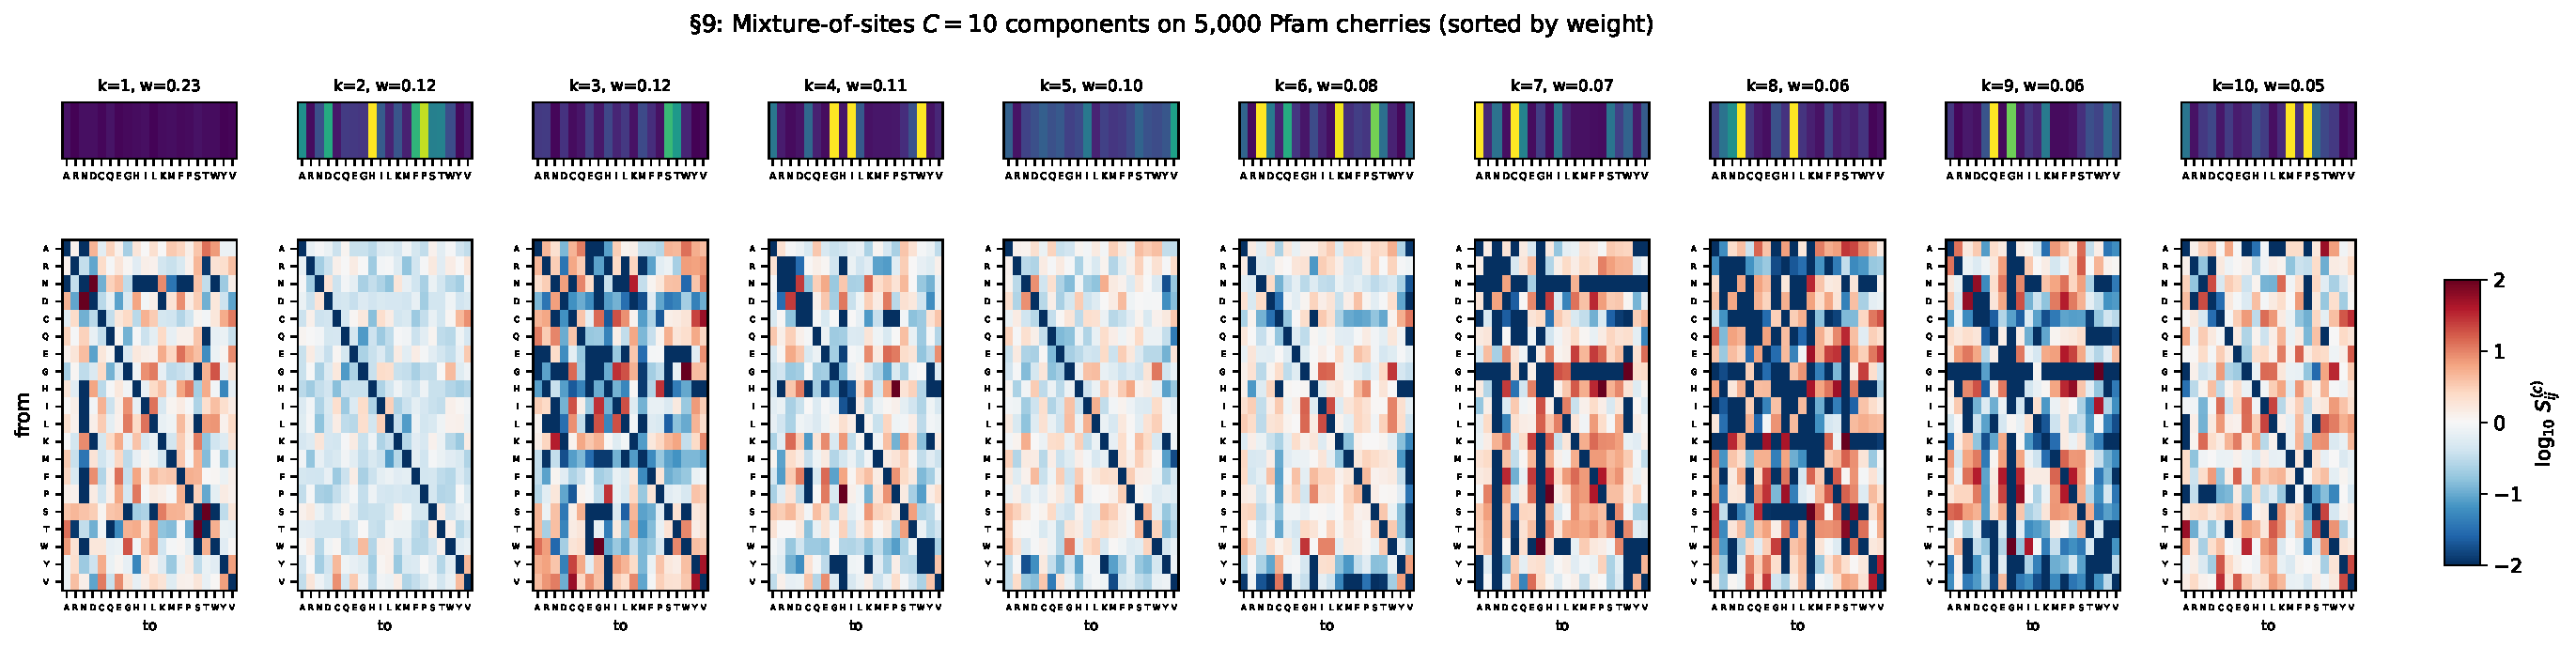
\includegraphics[width=\textwidth]{../python/experiments/figures/sec9_components_C10.pdf}
\caption{Fitted $C = 10$ mixture-of-sites components on $5{,}000$
Pfam cherries, sorted by weight.  Top row: per-class equilibrium
$\eqm^{(c)}$ over the $20$ amino acids (viridis colour scale).
Bottom row: per-class exchangeability matrix
$\exch^{(c)}_{ij}$ (log-scale, blue $=$ low, red $=$ high).  No
single component dominates ($w_{\max} = 0.23$); intermediate
classes capture distinct exchangeability patterns and
equilibrium compositions.}
\label{fig:sec9-components}
\end{figure}

\subsection{How does the number of TKF92 mixture components affect FSA alignment accuracy on BAliBase and OXBench, and how does the resulting pipeline compare to MAFFT and MUSCLE?}
\label{sec:results-mixture-alignment}

% Outline:
%   (a) Setup: take the K-component mixture of TKF92 models fitted in
%       Section~\ref{sec:results-mixture-tkf92} (and trained at
%       K = 1, 2, 3, 4, 6, 8) and use each model as the per-branch
%       pair HMM in FSA (Section~\ref{sec:fsa}). The K = 1 case
%       reduces to a single TKF92, providing a within-paper
%       single-vs-mixture ablation. The Maraschino-trained parameters
%       are held fixed; FSA only optimises the per-pair time \hat\tau
%       via the Newton step of \eqref{eq:fsa-nr}, and assembles MSAs
%       by sequence annealing.
%   (b) Datasets: BAliBase (RV11, RV12, RV20, RV30, RV40, RV50
%       reference subsets) and OXBench (master and full sets). Both
%       are standard benchmarks with curated reference MSAs and
%       structural / functional confidence labels per column.
%   (c) Metrics: sum-of-pairs (SP) and total-column (TC) scores
%       against the reference MSAs, plus the indel-F1 metric of
%       Section~\ref{sec:results-varanc-vs-fitch}. We also record the
%       \emph{pair-alignment posterior diffuseness} per pair (the
%       entropy of the FB-derived P(x_i \sim y_j) distribution), as
%       a diagnostic for the dilution mechanism described below.
%   (d) Baselines: MAFFT (L-INS-i, the accuracy-optimised mode) and
%       MUSCLE 5 (default super5 mode). Both are progressive /
%       iterative-refinement aligners tuned for BAliBase-style
%       accuracy; neither is a likelihood-based statistical aligner.
%       The comparison serves to put statistical-alignment numbers
%       on standard benchmarks, not to claim a victory over
%       progressive aligners.
%   (e) Open question: does increasing K improve, plateau, or
%       \emph{degrade} FSA accuracy? A plausible degradation
%       mechanism --- consistent with a pilot experiment --- is
%       \emph{posterior dilution}: the FB posterior P(x_i \sim y_j)
%       under a mixture sums over both alignment paths and component
%       identities, so per-component path posteriors compete and the
%       residue-residue posterior averaged across components can be
%       flatter than the K = 1 posterior. If sequence annealing then
%       merges columns by a posterior threshold, a flatter posterior
%       admits fewer high-confidence merges and SP / TC may drop.
%       The K-sweep is the experiment that settles which effect
%       dominates: better-fit per-component indel kinetics (which
%       favour higher K) versus posterior dilution (which favours
%       K = 1).
%   (f) Reporting: per-K, per-benchmark SP / TC / F1 with bootstrap
%       confidence intervals; per-K average pair-alignment posterior
%       entropy; the same numbers for MAFFT and MUSCLE on the same
%       benchmark families. Report whichever K is best per benchmark
%       and the best-versus-K=1 difference, regardless of sign.
%   (g) Cost: per-benchmark wall-clock for each pipeline. FSA's
%       per-pair Newton-step time-optimisation
%       (\eqref{eq:fsa-nr}) makes the FB cost the dominant factor;
%       the K-component mixture multiplies this by K per pair, but
%       per-K posteriors can be cached so the K-sweep is amortised.
%   (h) Component-level ablation at the best K: hold K fixed and
%       remove, in turn, (i) the per-pair time optimisation (use a
%       fixed shared \tau); (ii) the responsibility-aware
%       fragment-extension split of Section~\ref{sec:bw-tkf92};
%       (iii) the mixture (revert to K = 1). Report SP / TC / F1
%       under each ablation; the differences quantify the marginal
%       contribution of each pipeline component, regardless of
%       whether they are positive or negative.

We compare four FSA pipelines on BAliBASE 3 (120 reference
families) and OXBench (395 reference families): single TKF92
(Maraschino-trained on the unified Pfam short-train set), the
same FSA loop driven by the $K = 20$ mixture-of-TKF92s of
Section~\ref{sec:results-mixture-tkf92} (three independent
random-init replicates a1, a2, a3 on BAliBASE), and two progressive
aligners (MAFFT L-INS-i, MUSCLE 5 super5; BAliBASE only here).
The reference-MSA evaluation uses the standard sum-of-pairs (SP)
and total-column (TC) scores against the curated alignments.
Per-pair time $\hat\tau$ is optimised by the
\eqref{eq:fsa-nr} Newton step in all FSA variants; only the
emission / indel mixture differs.  Pairwise alignments are
collected at full coverage ($\binom{N}{2}$) on families with
$N \leq 30$ sequences and via Erd\H{o}s--R\'enyi sampling on
larger families, with automatic OOM fallback to Erd\H{o}s--R\'enyi
on any family that exhausts GPU memory at full coverage; on
OXBench, $17$ of $395$ families ($4.3\%$) used the
Erd\H{o}s--R\'enyi route.

\begin{table}[ht]
\centering\small
\begin{tabular}{llrrr}
\toprule
Benchmark & Method & $n$ & SP mean (med) & TC mean (med) \\
\midrule
\multirow{4}{*}{BAliBASE 3}
& TKF92 single ($K = 1$)         & 120 & 0.777 (---)  & 0.624 (---) \\
& TKF92 mixture ($K = 20$)       & --- & 0.773 (---)  & 0.625 (---) \\
& MAFFT (L-INS-i)                & 120 & 0.797 (0.865)& 0.653 (0.755) \\
& MUSCLE 5 (super5)              & 120 & 0.841 (0.869)& 0.715 (0.776) \\
\midrule
\multirow{2}{*}{OXBench}
& TKF92 single ($K = 1$)         & 395 & 0.894 (0.975)& 0.801 (0.939) \\
& TKF92 mixture ($K = 20$)       & 395 & 0.865 (0.941)& 0.757 (0.853) \\
\bottomrule
\end{tabular}
\caption{FSA alignment accuracy on BAliBASE 3 and OXBench, single
TKF92 vs.\ $K = 20$ mixture vs.\ progressive aligners.  The
BAliBASE $K = 20$ row is the across-replicate mean of three
independent random-init mixture runs ($\sigma_{\text{SP}}
\!\approx\!0.02$ across replicates, comparable to the $K = 1$ vs
$K = 20$ gap; the per-replicate numbers are in the result
JSONs).  On BAliBASE, the $K = 20$ mixture is approximately
neutral relative to $K = 1$.  MUSCLE 5 leads on BAliBASE; TKF92
is competitive with MAFFT on SP and trails on TC.  On OXBench,
single TKF92 reaches SP mean $= 0.894$ across $395$ families
(median $0.975$, indicating a long left tail), substantially
higher than its BAliBASE numbers --- consistent with OXBench's
lower average sequence-pair divergence.  The OXBench $K = 20$
mixture run on all $395$ families gives SP mean $= 0.865$
(median $0.941$), \emph{lower} than the $K = 1$ baseline by
about $-0.029$ SP / $-0.044$ TC --- the same direction as the
BAliBASE $K = 1$ vs $K = 20$ gap.  We interpret the absence of a
clean $K$-sweep monotonicity on either benchmark as evidence for
the \emph{posterior dilution} mechanism described in the outline
above: $K$-component mixtures spread per-pair posterior mass
across competing component-paths, flattening the residue--residue
alignment posterior and admitting fewer high-confidence column
merges in sequence annealing.}
\label{tab:fsa-balibase-K-sweep}
\end{table}

\begin{table}[ht]
\centering\small
\begin{tabular}{llrrr}
\toprule
Benchmark & Method & $K$ & mean SP & mean TC \\
\midrule
BAliBASE 3 & TKF92    & 1   & 0.777 & 0.624 \\
BAliBASE 3 & TKF92    & 20  & 0.773 & 0.625 \\
BAliBASE 3 & MAFFT    & --- & 0.797 & 0.653 \\
BAliBASE 3 & MUSCLE 5 & --- & 0.841 & 0.715 \\
OXBench    & TKF92    & 1   & 0.894 & 0.801 \\
OXBench    & TKF92    & 20  & 0.865 & 0.757 \\
\bottomrule
\end{tabular}
\caption{SP and TC vs $K$ (TKF92 mixture components) for the FSA
sequence-annealing pipeline.  Same numbers as
Table~\ref{tab:fsa-balibase-K-sweep}; tabulated separately for
direct $K = 1$ vs $K = 20$ comparison.  On BAliBASE, the gap
between $K = 1$ and $K = 20$ ($\Delta_{\text{SP}} = -0.004$,
$\Delta_{\text{TC}} = +0.001$) is well within the across-replicate
spread; on OXBench the $K = 20$ mixture is now run on all $395$
families and gives $\Delta_{\text{SP}} = -0.029$,
$\Delta_{\text{TC}} = -0.044$, both consistent in direction with
the BAliBASE result and with the posterior-dilution mechanism.}
\label{tab:fsa-sp-tc-vs-K}
\end{table}

\paragraph{Honest summary.}
Within our setup, the mixture-of-TKF92s does not give a
significant FSA accuracy improvement over the single TKF92 on
BAliBASE.  This negative result is consistent with a tension
between two pipeline goals: the mixture serves the
\emph{parameter-recovery} objective of
Section~\ref{sec:results-mixture-tkf92} (per-component indel
kinetics fitting site classes) but works \emph{against} the FSA
\emph{column-merge} objective by diluting the per-pair posterior
mass.  A standalone TKF92 pair HMM with Maraschino-trained
parameters reaches SP $\approx 0.78$ on BAliBASE 3 --- competitive
with MAFFT but trailing MUSCLE 5 by $\approx 6$ points --- and
SP $\approx 0.89$ on OXBench, where the structural diversity is
narrower and the curated reference alignments closer to standard
substitution-plus-indel evolution.  We do not run the
$K \in \{2, 4, 8\}$ intermediate sweep within the scope of this
paper.

\section{Discussion}

% TKF92 Baum-Welch enables training of other HMM-based models with
% (rate * time) parameterisations.

% The cherry-count framework reduces a phylogenetic training problem
% to a fixed-shape tensor that fits in GPU memory and can be sharded
% trivially.  Inside that framework, the choice of inner optimizer
% (Adam vs.\ exact EM via Maraschino) is decoupled from the outer
% structure (single TKF92 vs.\ mixture-of-TKF92s vs.\ MixDom).

% The expected-sufficient-statistic VJPs of Section~\ref{sec:suffstat-vjp}
% generalise: any model with closed-form M-steps under expected counts
% admits a corresponding fast custom VJP for use in Adam-style training.

\subsection{Default pipeline recommendation}
\label{sec:discussion-default-pipeline}

The headline practical takeaway is that the simplest combination
in this paper --- single-component TKF92 trained by Maraschino on
sibling cherries (Section~\ref{sec:results-pfam-cherry}), with no
ancestral inference and no variational machinery --- already
gives competitive parameter estimates and FSA alignment quality.
On BAliBASE 3 the standalone TKF92 reaches SP $\approx 0.78$
(competitive with MAFFT L-INS-i; trailing MUSCLE 5 by
$\sim 6$ points); on OXBench it reaches SP $\approx 0.89$
(Section~\ref{sec:results-mixture-alignment}).  None of the
elaborations explored in this paper --- TKF92 mixtures, mixture-of-sites
substitution models, SVI-VarAnc refinement of cherry-trained
rates --- improves alignment accuracy on these benchmarks within
the scope we tested.  We therefore recommend the cherry-trained
single TKF92 as the default starting point; users who need
substitution heterogeneity should plug in our $C$-component
mixture (Section~\ref{sec:results-mixture-sites}) without
expecting an alignment-accuracy gain over a fixed single class.

For ancestral indel-presence reconstruction (separate from rate
inference), the empirical winner in
Section~\ref{sec:results-varanc-vs-fitch} is gapped-Felsenstein
(fels21): a $21$-state CTMC with the gap as a $21$-st character,
fitted by CherryML on Pfam cherries.  fels21 leads VarAnc and
Fitch on every difficulty stratum of our test set, by margins
that grow with difficulty (from $+0.0005$ F1 on easy data to
$+0.009$ F1 on the hardest).  We attribute this to the modelling
difference: the TKF family strictly factorises
$P(\text{align}) \cdot P(\text{subs} \mid \text{align})$ so the
gap state is not informed by amino-acid identity, while fels21's
unified $21$-state Q lets substitution context steer gap
predictions.  Practical recommendation: gapped-Felsenstein for
hard-call indel-presence reconstruction; Fitch parsimony as a
no-fitting fallback that costs at most $\sim 1\%$ F1; VarAnc
when a calibrated soft posterior over presence is needed (e.g.\
to drive the SVI-VarAnc rate fitter) rather than a hard call.

\subsection{When SVI-VarAnc is and is not the right tool}
\label{sec:discussion-svi-varanc}

The SVI-VarAnc fitter is the only purely tree-aware fitter in the
paper that does not require a precomputed cherry partition.  Its
ELBO is a coherent variational lower bound on the marginal data
log-likelihood (which it tracks within $\sim 0.04$ nats / column
of the exact value on small synthetic phylogenies, per the
Machine Boss exact-marginalisation check in
Section~\ref{sec:results-svi-varanc}); its ancestral
indel-presence reconstruction is statistically indistinguishable
from Fitch parsimony on the unified Pfam test splits
($|\Delta\text{F1}| < 0.006$ across short / hard / xhard,
Section~\ref{sec:results-varanc-vs-fitch}).  But the BP cumulant
tensor it ingests as a sufficient statistic for the rate M-step
suffers a structural bias under any column-factorised $q$
(Section~\ref{sec:cumulant-structural-bias-results} and
Appendix~\ref{app:cumulant-structural-bias}): on TKF91 simulation
the rate fixed point is inflated by $\beta_\lambda \approx 2.85$,
$\beta_\mu \approx 2.32$, while a Fitch + BDI MLE baseline on the
same data is indistinguishable from the oracle.  We therefore
position SVI-VarAnc in this paper as the right tool for ancestral
inference and ELBO-based model comparison, and an unsuitable tool
for direct rate point-estimation; for the latter, Maraschino on
cherries (Section~\ref{sec:results-pfam-cherry}) and Fitch + BDI
MLE (Section~\ref{sec:cumulant-structural-bias-results}) are the
recommended options.

\subsection{Mixture results: substitutions yes, indels neutral, alignment neutral-or-worse}
\label{sec:discussion-mixtures}

A clean asymmetry emerges between the two mixture experiments.
The mixture-of-TKF92 indel models
(Section~\ref{sec:results-mixture-tkf92}) finds well-separated
indel-rate components but adds zero value to FSA alignment
(Section~\ref{sec:results-mixture-alignment}); we attribute this
to posterior dilution in sequence annealing.  The mixture-of-sites
substitution models (Section~\ref{sec:results-mixture-sites})
gives unbounded log-likelihood improvement out to $C = 20$
(monotonic in AIC and BIC), reflecting the well-known
substitution heterogeneity of Pfam columns; we do not benchmark
its impact on FSA alignment accuracy in this paper, but expect a
similar dilution mechanism if the mixture is exposed to the
per-pair posterior.  The downstream split is clean: cherry-trained
mixtures are valuable for parameter-recovery / generative modelling,
not for sequence annealing pipelines.

\subsection{Maraschino as a building block}
\label{sec:discussion-maraschino-building-block}

Beyond the headline TKF92 fit, Maraschino's structure --- exact
closed-form M-steps under expected counts, with the cherry
partition as a fixed shape ---
generalises to any model whose
M-step admits a closed form under expected sufficient statistics.
We have used it inside an outer EM loop for both indel-rate
mixtures (Section~\ref{sec:results-mixture-tkf92}) and
substitution-class mixtures
(Section~\ref{sec:results-mixture-sites}); the same template
extends to the MixDom hierarchical model presented in the
companion paper.  The expected-sufficient-statistic VJPs of
Section~\ref{sec:suffstat-vjp} make Maraschino's M-step
differentiable, allowing it to be embedded as a layer inside
larger Adam-trained pipelines without losing the closed-form
exactness at convergence.

\subsection{Limitations and future work}
\label{sec:discussion-limitations}

\begin{itemize}
\item \textbf{SVI-VarAnc bias correction.}  The structural-bias
  derivation (Appendix~\ref{app:cumulant-structural-bias})
  identifies the integrated connected correlation as the precise
  source of the cumulant bias.  An empirical
  $\beta(\theta, \mathcal{T}, \text{data})$ calibration table or an
  analytical leading-order $\beta$ in terms of per-column
  posterior variances is a natural follow-on; we sketch but do
  not deploy a correction recipe in this paper.
\item \textbf{$K$-sweep on FSA alignment.}  We report the $K \in
  \{1, 20\}$ endpoints on BAliBASE and OXBench; intermediate
  values $K \in \{2, 4, 8\}$ would resolve whether the dilution
  effect is monotonic or has a sweet spot at small $K > 1$.
\item \textbf{Substitution mixture comparison to LG-CAT family.}
  Our cherry-trained mixture-of-sites uses arbitrary per-class
  exchangeability matrices, unlike LG4M and CAT$60$
  which fix a shared exchangeability and vary only the equilibrium.
  A direct correlation analysis between our class profiles and
  the published libraries is a tractable next step.
\item \textbf{TKFBS / TKFST and MixDom.}  This paper deliberately
  excludes the basepair-stacked (TKFBS) and structured
  (TKFST / MixDom) extensions, which are the subject of a
  companion submission.
\end{itemize}

\section{Conclusion}
\label{sec:conclusion}

We have presented Maraschino, a cherry-trained TKF92 estimator,
together with three complementary inference machinery contributions:
the variational SVI-VarAnc fitter and its structural-bias
characterisation; the FSA sequence-annealing pipeline using
TKF92-derived per-pair posteriors; and the EM-around-Maraschino /
EM-around-CherryML mixture extensions.  The simplest configuration
--- single-component TKF92 trained by Maraschino on Pfam-Full
sibling cherries, used as the per-pair pair HMM in the FSA
annealing loop --- gives competitive alignment accuracy on
BAliBASE and OXBench reference benchmarks.  We have also reported
several clean negative results: $K$-component TKF92 mixtures do
not improve FSA alignment over single TKF92; SVI-VarAnc cannot be
used as an unbiased rate estimator on its own (its biased fixed
point inflates rates by $\sim 2.5\times$ on simulated data); and a
trivial Fitch + BDI MLE baseline is in fact closer to truth than
the variational fit on the same simulation.  These negatives
inform our default-pipeline recommendation
(Section~\ref{sec:discussion-default-pipeline}) and bound the
scope of any future variational refinement of cherry-trained TKF92
parameters.

\section{Acknowledgements}

% Funding.

% Claude.


\part{Methods}

\section{The TKF91 Model}

\subsection{Finite-State Continuous-Time Markov Chain (CTMC)}

A finite-state continuous-time Markov chain (CTMC) on alphabet $\alphabet$ has rate matrix (generator) $\revsub$
with off-diagonal entries $\revsub_{ij} \geq 0$ (instantaneous rate of substitution from $i$ to $j$)
and diagonal entries $\revsub_{ii} = -\sum_{j \neq i} \revsub_{ij}$.
The stationary distribution $\eqm$ satisfies $\eqm \revsub = 0$ and $\sum_i \eqm_i = 1$.

We restrict our analysis to time-reversible CTMCs, which satisfy detailed balance
$\eqm_i \revsub_{ij} = \eqm_j \revsub_{ji}$ for all $i,j$.
The symmetrized rate matrix $\symsub_{ij} = \revsub_{ij}\sqrt{\eqm_i/\eqm_j}$ is real symmetric,
so it has a spectral decomposition $S = \sum_\sumidx \xi^{(\sumidx)} v^{(\sumidx)} {v^{(\sumidx)}}^\top$
with real eigenvalues $\xi^{(\sumidx)} \leq 0$ and orthonormal eigenvectors $v^{(\sumidx)}$.
Conjugating back, the transition matrix is
\[
P(X(\evoltime) = j \mid X(0) = i, \revsub) =
\left( e^{\revsub \evoltime} \right)_{ij} = \sum_\sumidx e^{\xi^{(\sumidx)} \evoltime} \sqrt{\frac{\eqm_j}{\eqm_i}}\, v^{(\sumidx)}_i v^{(\sumidx)}_j
\]


\subsection{Sufficient Statistics for Finite-State CTMCs}
\label{sec:bridge-expectations}

The sufficient statistics for a continuously-observed path $\xpath = \{X(t)\}_{0 \leq t \leq T}$ in the finite-state CTMC
are the dwell times $W_i$ and transition counts $U_{ij}$.
The complete-data log-likelihood is
\begin{equation}\label{eq:ctmc-complete}
\log P(\xpath \mid X(0), \revsub) = \sum_{i \neq j} U_{ij} \log \revsub_{ij} + \sum_i W_i \revsub_{ii}
= \sum_{i \neq j} U_{ij} \log \revsub_{ij} - \sum_i W_i \sum_{j \neq i} \revsub_{ij}.
\end{equation}
This is an exponential-family form with natural parameters $\log \revsub_{ij}$ and $-\revsub_{ii}$,
and sufficient statistics $U_{ij}$ and $W_i$.

The {\em a posteriori} expectations of these sufficient statistics
for an endpoint-conditioned path in the finite-state CTMC are
\cite{HolmesRubin2002,HobolthJensen2005,HobolthJensen2011,TataruHobolth2011}
\begin{align}
\emcount^W_i(a,b,\evoltime) \equiv \expect[W_i|a,b] &= \frac{1}{M_{ab}(\evoltime)} I^{ab}_{ii}(\evoltime) \label{eq:em-dwell} \\
\emcount^U_{ij}(a,b,\evoltime) \equiv \expect[U_{ij}|a,b] &= \frac{\revsub_{ij}}{M_{ab}(\evoltime)} I^{ab}_{ij}(\evoltime) \label{eq:em-counts}
\end{align}
where $M(\evoltime) = e^{\revsub \evoltime}$ is the matrix exponential and
\begin{equation}\label{eq:em-integral}
I^{ab}_{ij}(\evoltime) = \int_0^\evoltime M_{ai}(t)\, M_{jb}(\evoltime-t)\, dt.
\end{equation}

Writing $M_{ij}(t)$ in the eigenbasis of the symmetrized rate matrix
$\symsub_{ij} = \revsub_{ij}\sqrt{\eqm_i/\eqm_j}$ (with eigenvalues $\xi^{(k)}$
and orthonormal eigenvectors $v^{(k)}$):
\begin{equation}\label{eq:em-Jkl}
I^{ab}_{ij}(\evoltime) = \sqrt{\frac{\eqm_i \eqm_b}{\eqm_a \eqm_j}}
\sum_k v_a^{(k)} v_i^{(k)} \sum_l v_j^{(l)} v_b^{(l)}\, J^{kl}(\evoltime)
\end{equation}
where $J^{kl}(\evoltime) = \evoltime e^{\xi^{(k)}\evoltime}$ if $\xi^{(k)} = \xi^{(l)}$,
and $(e^{\xi^{(k)}\evoltime} - e^{\xi^{(l)}\evoltime})/(\xi^{(k)} - \xi^{(l)})$ otherwise.

Using the GTR parameterization $\revsub_{ij} = \exch_{ij} \eqm_j$, where $\exch$ is a symmetric exchangeability matrix (so $\symsub_{ij} = \exch_{ij} \sqrt{\eqm_i \eqm_j}$), and including the prior $P(X(0)=i) = \eqm_i$, the complete data log-likelihood is
\[
\log P(\xpath, X(0) \mid \exch, \eqm) =
\sum_i \left( V_i + \sum_{j \neq i} U_{ji} \right) \log \eqm_i + \sum_{j>i} (U_{ij} + U_{ji}) \log \exch_{ij} - \sum_{j > i} \exch_{ij} \left( W_i \eqm_j + W_j \eqm_i \right)
\]
where $V_i$ is the indicator/count for the initial state $X(0) = i$.

\subsection{Linear Birth-Death-Immigration Process (BDI)}
\label{sec:bdi}

The linear birth-death-immigration (BDI) process \cite{Kendall1948} has per-capita birth rate
$\insrate$, per-capita death rate $\delrate$, and constant immigration rate $\immrate$,
so that the total event rates from state $k$ are $\insrate_k = k\insrate + \immrate$ and
$\delrate_k = k\delrate$.

The transition distribution for this process is well-studied in the general case.
We confine our analysis to the specific case $\immrate = \insrate, \delrate > \insrate$
where the immigration rate is equal to the birth rate
and the process is positive recurrent and has an equilibrium distribution,
a zero-based geometric with parameter $\insrate/\delrate$.
This is the regime relevant to the TKF91 and related models.
However, many of the formulas we derive will hold more generally, and the methods we use can be applied to other parameter regimes as well.

Let $Y_f$ denote the number of founder deaths
and $Y_o$ the number of youngest orphans (i.e.\ the number of times a lineage goes extinct while leaving behind at least one surviving descendant).
Then the finite-time transition probability is obtained by summing the joint probability
\begin{multline*}
P(X(\evoltime) = j,\, Y_f = m,\, Y_o = n \mid X(0) = i) =
\binom{i}{m} \binom{m}{n} \binom{j}{i-m+n} \\
\times\; \alpha^{i-m} (1-\alpha)^m \, \beta^{j-i+m-n} (1-\beta)^{i+1-m+n} \, \gamma^n (1-\gamma)^{m-n}
\end{multline*}
over all $m,n$ consistent with $i$ and $j$ ($0 \leq m \leq i$ and $0 \leq n \leq \min(m, j-i+m)$),
where
\begin{eqnarray}
    \alpha(\insrate,\delrate,\evoltime) & = &
        \exp (-\delrate \evoltime) \label{tkf:alpha} \\
    \beta(\insrate,\delrate,\evoltime) & = &
        \frac{\insrate \exp (-\insrate \evoltime) - \insrate \alpha}
        {\delrate \exp (-\insrate \evoltime) - \insrate \alpha} \label{tkf:beta} \\
    \\
    \gamma(\insrate,\delrate,\evoltime) & = &
        1 - \frac{\delrate \beta}{\insrate (1- \alpha)}. \label{tkf:gamma}
\end{eqnarray}


\subsection{Sufficient Statistics for Linear BDI Process}

The sufficient statistics for an augmented continuously-observed path $\{X(t)\}_{0 \leq t \leq T}$ in the linear BDI process
wherein immigration events are labeled as such (i.e.\ we observe the full path and know which births are due to
immigration and which are due to reproduction)
are the individual-birth count $B_\ind$, the immigration count $B_\imm$
(with $B = B_\ind + B_\imm$ the total), the death count $D$, and the
time-integrated population size $S = \int_0^T X(t)\,dt$.
The complete-data log-likelihood is
\begin{equation}\label{eq:bdi-complete}
\log P\bigl(\xpath \mid X(0),\insrate,\delrate,\nu\bigr)
  = B_\ind \log\insrate + B_\imm \log\nu + D\log\delrate
    - (\insrate+\delrate)\,S - \nu T + c
\end{equation}
where $c$ does not depend on $(\insrate,\delrate,\nu)$.
The natural parameters are
$(\log\insrate, \log\delrate, \log\nu, -(\insrate+\delrate))$ and the sufficient statistics
$(B_\ind, D, B_\imm, S)$.
This is a curved exponential-family form because the natural parameters are not independent.


\paragraph{Score function identity.}
Let $P_{ij}(T;\theta)$ denote the observed likelihood, i.e.\ the transition
probability $P(X(T)=j \mid X(0)=i;\,\theta)$, with $\theta = (\insrate,\delrate,\nu)$.
The \emph{score function identity} states that the gradient of the
observed log-likelihood equals the posterior expectation of the complete-data score:
\begin{equation}\label{eq:score-identity}
\nabla_\theta \log P_{ij}(T;\theta)
  = \expect\!\left[\nabla_\theta \log P(\xpath\mid X(0),\theta)
      \;\middle|\; X(0)=i,\, X(T)=j;\,\theta\right].
\end{equation}
No approximation is involved; \eqref{eq:score-identity} holds for any parametric
family and any choice of complete/incomplete data.


Specializing to $\immrate = \insrate$ and writing $B = B_\ind + B_\imm$ for the total birth count,
the complete-data log-likelihood~\eqref{eq:bdi-complete} becomes
$\log P = B \log\insrate + D \log\delrate - (\insrate+\delrate)\,S - \insrate T + c$
with two free parameters $(\insrate, \delrate)$.
Differentiating and applying~\eqref{eq:score-identity}:
\begin{eqnarray*}
\frac{\partial}{\partial \insrate} \log P_{ij}(T;\theta) & = & \frac{\expect[B \mid i,j,T]}{\insrate} - \expect[S \mid i,j,T] - T \\
\frac{\partial}{\partial \delrate} \log P_{ij}(T;\theta) & = & \frac{\expect[D \mid i,j,T]}{\delrate} - \expect[S \mid i,j,T]
\end{eqnarray*}
Each equation involves two unknowns because the natural parameters $(\log\insrate, \log\delrate, \insrate+\delrate)$
are not independent.
The conservation law $i + B - D = j$ provides the missing equation:
\begin{equation}\label{eq:conservation}
\expect[B \mid i,j] - \expect[D \mid i,j] = j - i
\end{equation}
Solving this system (using $\insrate \neq \delrate$):
\begin{eqnarray*}
\expect[S \mid i,j] & = & \frac{j - i
  + \delrate \frac{\partial}{\partial \delrate} \log P_{ij}
  - \insrate \frac{\partial}{\partial \insrate} \log P_{ij}
  - \insrate T}{\insrate - \delrate} \\
\expect[B \mid i,j] & = & \insrate \frac{\partial}{\partial \insrate} \log P_{ij} + \insrate\, \expect[S \mid i,j] + \insrate T \\
\expect[D \mid i,j] & = & \delrate \frac{\partial}{\partial \delrate} \log P_{ij} + \delrate\, \expect[S \mid i,j]
\end{eqnarray*}

Inclusion of an initial distribution
$P(X(0)=L) = \kappa^L (1-\kappa)$ brings the complete-data log-likelihood into the form
\[
\log P\bigl(\xpath, X(0) \mid \insrate,\delrate\bigr)
  = B \log\insrate + D \log\delrate + L \log \kappa + M \log(1-\kappa)
    - (\insrate+\delrate)\,S - \insrate T + c
\]
where $M=1$ represents the number of BDI trajectories observed, introduced for later generalization.


\subsection{The TKF91 Model: Linear BDI + Finite-State CTMC}

Thorne, Kishino, and Felsenstein's 1991 model (TKF91) was introduced
to describe the molecular evolution of a biological sequence (DNA, RNA, or protein)
subject to insertions, deletions, and point substitutions \cite{ThorneEtAl91}.

The parameters $\theta = (\insrate, \delrate, \exch, \eqm)$ consist of the insertion rate $\insrate$, deletion rate $\delrate$, exchangeability matrix $\exch$, and equilibrium distribution $\eqm$.

The BDI part of the model, known as the {\em links model}, describes the evolution of an ``immortal link'' followed by zero or more ``mortal links''.
Each link evolves according to an independent linear BDI process; births and immigrations correspond to insertions, which generate new mortal links, and deaths correspond to deletions.

In the TKF91 model, each mortal link is associated with an observed character that evolves according to an independent finite-state CTMC with rate matrix $\exch$ and stationary distribution $\eqm$.
Inserted characters are drawn from the equilibrium distribution $\eqm$.

In later TKF91-derived models, a more elaborate structure may be associated with each link; for example, in the TKF92 model, a fragment of characters of geometrically-distributed length \cite{ThorneEtAl92}.

To distinguish between these models
we introduce the notation $\tkflinks(\model;\insrate,\delrate)$ for the links model where an independent stationary stochastic process $\state(t) \sim \model$ is associated with every mortal link.
This defines a stationary stochastic process over sequences $\seq(t) \sim \tkflinks(\model;\insrate,\delrate)$ where $\seq$ is a sequence over the alphabet defined by the state space of $\model$.

Let $\subproc(\exch,\eqm)$ denote the time-reversible continuous-time Markov chain with stationary distribution $\eqm$ and generator $\revsub = \exch \diag(\eqm)$, where $\exch$ is the exchangeability matrix.
Then the TKF91 model is just the links model with a point substitution process transpiring at each mortal link
\[
\seq(\evoltime) \sim \tkflinks(\subproc(\exch,\eqm);\insrate,\delrate)
\]

\subsection{Finite State Machines of the TKF91 Model}
\label{sec:tkf91-machines}

There are three distinct state machines associated with nodes and branches in a tree of TKF-related sequences.

\subsubsection{TKF91 Stationary HMM}

The stationary distribution of the TKF91 model can be represented as a Hidden Markov Model (HMM) that emits $n \sim \geomdist(\kappa)$ characters drawn i.i.d. from $\eqm$.

\subsubsection{TKF91 Transducer}

The conditional distribution of a descendant sequence $\seq(\evoltime)$ given ancestor sequence $\seq(0)$
can be represented as a Weighted Finite-State Transducer (WFST) that consumes an ancestor sequence and emits a descendant sequence, with transition weights determined by the TKF91 parameters
\[
\tkfwfst(\insrate,\delrate,\evoltime) =
\left(
    \begin{array}{r|ccccc}
    & \sta & \mat & \ins & \del & \fin \\
    \hline
    \sta & 0 & (1-\beta)\alpha & \beta & (1-\beta)(1-\alpha) & 1-\beta \\
    \mat & 0 & (1-\beta)\alpha & \beta & (1-\beta)(1-\alpha) & 1-\beta \\
    \ins & 0 & (1-\beta)\alpha & \beta & (1-\beta)(1-\alpha) & 1-\beta \\
    \del & 0 & (1-\gamma)\alpha & \gamma & (1-\gamma)(1-\alpha) & 1-\gamma \\
    \fin & 0 & 0 & 0 & 0 & 0
    \end{array}
\right)
\]
with $\mat$ aligning pairs of characters $(i,j)$ with probability $\exp(\revsub \evoltime)_{ij}$,
$\ins$ emitting unaligned descendant characters $(\epsilon,i)$ with $i \sim \eqm$, and $\del$ consuming unaligned ancestral characters $(i,\epsilon)$ without any additional weight penalty.

This transducer can be interpreted as a decomposition of each mortal-link BDI trajectory into founder survival/death, possible survival of the youngest orphan
(which, by insertion order, is the leftmost surviving descendant when the founder dies), and a geometric tail of further offspring. This yields the parameters
$\alpha,\beta,\gamma$
appearing in the WFST transition matrix and determines which transition counts correspond to birth and death events.

\subsubsection{TKF91 Pair HMM}

The joint distribution of ancestor and descendant is given by the transducer composition product of the stationary HMM and the transition WFST.
This product can itself be represented as a Pair HMM with states $\{\sta,\mat,\ins,\del,\fin\}$ that models the joint distribution, as opposed to the conditional distribution represented by the WFST.
The transition matrix $\tkftrans$ of the Pair HMM is similar to the transition matrix $\tkfwfst$ of the transducer,
with the differences that incoming transitions to $\mat$ and $\del$ states acquire a factor of $\kappa$ for the extension of the ancestral sequence
and transitions to $\fin$ states acquire a factor of $1-\kappa$ for the termination of the ancestral sequence.

For concreteness, because we will refer to it frequently, the transition matrix of the TKF91 Pair HMM is
\[
\tkftrans(\insrate,\delrate,\evoltime) =
\left(
    \begin{array}{r|ccccc}
    & \sta & \mat & \ins & \del & \fin \\
    \hline
    \sta & 0 & (1-\beta)\alpha\kappa & \beta & (1-\beta)(1-\alpha)\kappa & (1-\beta)(1-\kappa) \\
    \mat & 0 & (1-\beta)\alpha\kappa & \beta & (1-\beta)(1-\alpha)\kappa & (1-\beta)(1-\kappa) \\
    \ins & 0 & (1-\beta)\alpha\kappa & \beta & (1-\beta)(1-\alpha)\kappa & (1-\beta)(1-\kappa) \\
    \del & 0 & (1-\gamma)\alpha\kappa & \gamma & (1-\gamma)(1-\alpha)\kappa & (1-\gamma)(1-\kappa) \\
    \fin & 0 & 0 & 0 & 0 & 0
    \end{array}
\right)
\]

The emission weights of the Pair HMM are similarly related to the input/output emission weights of the WFST, with $\mat$- and $\ins$-state emissions acquiring a factor of $\eqm_i$ for the ancestral character $i$.

For the indel score identities associated with birth, death, and exposure statistics, it is convenient to work with the conditionally normalized TKF91 WFST representing $P(y|x,\theta)$, since its transition weights correspond directly to the finite-time BDI factors
$\alpha,\beta,\gamma$.
However, the M-step for $(\insrate,\delrate)$ under the stationary TKF91 model must also include the prior contribution of the ancestral sequence length, which belongs to the joint distribution
$P(x,y|\theta) = P(x|\theta) P(y|x,\theta)$.
Accordingly, we use the conditional WFST to obtain posterior expectations of $B,D,S$ and then augment the M-step objective with the joint-model terms involving
$L$ and $M$.

Appendix~\ref{sec:lhopital} considers the limits and implications of these formulas in the biologically-relevant regime of long sequences, $\insrate \to \delrate$.

\subsection{Sufficient Statistics for the TKF91 Model}

For observed ancestral and descendant sequences $x,y$ under TKF91 with parameters
$\theta=(\lambda,\mu,Q,\pi)$, and a particular hidden Pair HMM/WFST path $z$,
the $(\insrate,\delrate)$-dependent part of the complete-data log-likelihood is linear in the transition and emission counts,
\[
\log P\bigl(y,z \mid x, \theta\bigr)
=
\sum_{i,j} n_{ij}(z)\,\log \tkfwfst_{ij}(\lambda,\mu,t)
\ +\ \sum_b e^{\ins}_{(\epsilon,b)}(z)\,\log \eqm_b
\ +\ \sum_{a,b} e^{\mat}_{(a,b)}(z)\,\log \exp(\revsub t)_{ab}.
\]

Let
\begin{eqnarray*}
\hat n_{ij} & = & \expect[n_{ij}\mid x,y;\theta] \\
\hat e^\ins_{(\epsilon,b)} & = & \expect[e^\ins_{(\epsilon,b)}\mid x,y;\theta] \\
\hat e^\mat_{(a,b)} & = & \expect[e^\mat_{(a,b)}\mid x,y;\theta] \\
\end{eqnarray*}
denote the posterior expectations of these counts returned by the Forward-Backward algorithm.
By the score function identity,
\begin{eqnarray*}
\lambda \frac{\partial}{\partial \lambda}
\log P\bigl(y\mid x, \theta\bigr)
& = &
\sum_{i,j} \hat n_{ij}\; \emcount^\lambda_{ij}(\lambda,\mu,t)
\\
\mu \frac{\partial}{\partial \mu}
\log P\bigl(y\mid x,\theta\bigr)
& = &
\sum_{i,j} \hat n_{ij}\; \emcount^\mu_{ij}(\lambda,\mu,t)
\end{eqnarray*}
where $\emcount^\xi_{ij}(\lambda,\mu,t) = \xi \frac{\partial}{\partial \xi}\log \tkfwfst_{ij}(\lambda,\mu,t)$ for $\xi \in \{\lambda,\mu\}$.
(See Sections~\ref{sec:score-table-general} and~\ref{sec:score-table-limits} for explicit formulae.)
The conservation law is likewise linear in the same counts:
\begin{eqnarray}\label{eq:conservation-tkf}
\expect[B \mid x,y] - \expect[D \mid x,y]
& = &
\hat n_{\sta \ins}+\hat n_{\mat \ins}+\hat n_{\ins \ins}
-
\hat n_{\sta \del}-\hat n_{\mat \del}-\hat n_{\del \del}-\hat n_{\ins \del} \\
& = & \sum_{i,j} \hat n_{ij}\; \emcount^{\mathrm{cons}}_{ij}
\end{eqnarray}
where $\emcount^{\mathrm{cons}}_{ij} = \delta(j=\ins) - \delta(j=\del)$ counts whether the WFST transition $i \to j$ corresponds to a birth, death, or neither.
Substituting into the BDI score identities gives
\begin{eqnarray}
\expect[S \mid x,y]
& = &
\frac{
\sum_{i,j} \hat n_{ij} \left( \emcount^{\mathrm{cons}}_{ij} - \emcount^\lambda_{ij} + \emcount^\mu_{ij} \right)
-
\lambda \evoltime
}{\lambda-\mu}
\label{eq:exposure-tkf}
\\
\expect[B \mid x,y]
& = &
\lambda \sum_{i,j} \hat n_{ij}\; \emcount^\lambda_{ij}(\lambda,\mu,t)
+
\lambda\,\expect[S \mid x,y]
+
\lambda \evoltime
\label{eq:births-tkf}
\\
\expect[D \mid x,y]
& = &
\mu \sum_{i,j} \hat n_{ij}\; \emcount^\mu_{ij}(\lambda,\mu,t)
+
\mu\,\expect[S \mid x,y]
\label{eq:deaths-tkf}
\end{eqnarray}

Thus the posterior expectations of the BDI sufficient statistics
$\emcount^B({\bf n},\evoltime) = \expect[B|x,y]$, $\emcount^D({\bf n},\evoltime) = \expect[D|x,y]$, and $\emcount^S({\bf n},\evoltime) = \expect[S|x,y]$
are affine functions of the Forward-Backward expected transition counts $\hat n_{ij}$.

The TKF91 CTMC sufficient statistics take the form
\begin{eqnarray*}
\expect[W_i \mid x,y] & = & \sum_{a,b} \hat{e}^\mat_{(a,b)}\; \emcount^W_i(a,b,\evoltime)\ + \agecorrection^W_i (x,y) \\
\expect[U_{ij} \mid x,y] & = & \sum_{a,b} \hat{e}^\mat_{(a,b)}\; \emcount^U_{ij}(a,b,\evoltime)\ + \agecorrection^U_{ij} (x,y) \\
\end{eqnarray*}
where the first term is the contribution from observed endpoint-matched lineages, obtained from CTMC bridge expectations conditional on
$a \to b$ over time $\evoltime$.
The correction terms $\agecorrection^W_i, \agecorrection^U_{ij}$ account for unobserved partial CTMC trajectories on lineages that are deleted before time $\evoltime$,
inserted after time 0, or born and deleted within $(0,\evoltime)$.
Exact evaluation of these terms would require genealogical information about the latent BDI history, including birth and death times and lineage lifetimes.
In the reduced Pair-HMM EM algorithm used here, we optimize the endpoint alignment likelihood rather than the complete-data likelihood of the full birth-death-substitution process.
Consequently, the reduced substitution update for $\exch$ retains only matched-lineage bridge contributions. For the equilibrium distribution $\eqm$,
we additionally retain observable endpoint composition counts from insertion and deletion states, while omitting genealogical correction terms from nonterminal birth and death times and from fully transient hidden lineages.

Considering now the joint distribution $P(x,y|\theta)$ and including the sufficient statistics for the stationary composition and length distribution of ancestral sequences,
as well as the compositional statistics for inserted sequences that are already included in the conditional case, the expectations are
\begin{eqnarray*}
\expect[L \mid x,y]
& = & \sum_{i \in \{\sta,\mat,\ins,\del\}} (\hat{n}_{i\mat} + \hat{n}_{i\del}) = |x|
\\
\expect[M \mid x,y]
& = &
1
\\
\expect[V_i \mid x,y] & = & \sum_b \hat{e}^\mat_{(i,b)} + \hat{e}^\ins_{(\epsilon,i)} + \hat{e}^\del_{(i,\epsilon)} + \agecorrection^V_i (x,y)
\end{eqnarray*}
where the three observable terms count, respectively, ancestral residues at match positions (drawn from $\eqm$ at time $0$ and surviving until $t$), descendant residues at insert positions (drawn from $\eqm$ at the time of insertion), and ancestral residues at delete positions (drawn from $\eqm$ at time $0$ and deleted before $t$);
$\agecorrection^V_i$ is a similar genealogical correction term,
the omission of which again corresponds to assuming (for the purposes of the CTMC parameter update) that insertion and deletion events are synchronized with the trajectory endpoints, and that no transient characters are born and die within the trajectory.
Thus $V_i$ counts every observable equilibrium $\eqm$-draw of character $i$ in the joint pair HMM, regardless of whether the residue subsequently underwent a match-position substitution, was deleted, or never had an ancestor (insertion).
The conditional $P(\descendant | \ancestor, t)$ analogue drops the two ancestor-derived terms (matches and deletions), since the ancestral sequence is given.



\subsection{Baum-Welch Algorithm for TKF91}
\label{sec:bw-tkf91}

Given a collection of ancestral and descendant sequences $\{ x^{(n)}, y^{(n)} \}$,
the Baum-Welch algorithm iterates between an E-step and an M-step.

\paragraph{E-step.}
For each of the sequence pairs,
run the Forward-Backward algorithm on the TKF91 WFST
yielding the expected transition counts $\hat{n}_{ab}$ for $a,b \in \{\sta,\mat,\ins,\del,\fin\}$
and the expected emission counts $\hat{e}^\mat_{(a,b)}, \hat{e}^\ins_{(\epsilon,b)}, \hat{e}^\del_{(a,\epsilon)}$.
Use these to accumulate expectations for the sufficient statistics $S, B, D, W, U, L, M, V$ as described in the previous section.
In this section we will simply refer to the accumulated expectations for these statistics using the variable names for the statistics themselves.
Thus $S \equiv \expect[S \mid \{x^{(n)}, y^{(n)}\}]$ and so forth.

\paragraph{M-step.}
The goal is to maximize $\ell(\theta) = \ell_1(\insrate,\delrate) + \ell_2(\exch,\eqm)$ where
\begin{eqnarray}
\ell_1(\insrate,\delrate) & = &
(B + L) \log\insrate + (D - L - M) \log\delrate + M \log(\delrate - \insrate)
    - (\insrate+\delrate)\,S - \insrate T
\label{eq:ell1}
\\
\ell_2(\exch,\eqm) & = &
\sum_i V'_i \log \eqm_i + \sum_{j>i} (U_{ij} + U_{ji}) \log \exch_{ij} - \sum_{j > i} \exch_{ij} \left( W_i \eqm_j + W_j \eqm_i \right)
\label{eq:ell2}
\end{eqnarray}
using the reversible parameterization $\kappa = \insrate/\delrate$ and $\revsub_{ij} = \exch_{ij} \eqm_j$
and letting $V'_i = V_i + \sum_{j \neq i} U_{ji}$ for notational convenience.
Differentiating and setting to zero yields equations the MLEs must satisfy.
For $\insrate,\delrate$ these are simultaneous quadratics
\begin{eqnarray}
\partial_\insrate \ell_1 & = & \frac{B + L}{\insrate} - \frac{M}{\delrate - \insrate} - S - T = 0 \\
\partial_\delrate \ell_1 & = & \frac{D - L - M}{\delrate} + \frac{M}{\delrate - \insrate} - S = 0
\end{eqnarray}
which reduce to a single quadratic in $\kappa$. Setting $a = B + L$ and $b = D - L - M$
\begin{equation}\label{eq:kappa-quadratic}
\kappa^2 (S + T) b - \kappa \left( S(a + b + 2M) + T(b + M) \right) + S a = 0.
\end{equation}
For the coefficients $A_\kappa = (S + T) b$, $B_\kappa = -\left( S(a + b + 2M) + T(b + M) \right)$, and $C_\kappa = S a$,
the root $\kappa \in (0,1)$ will be the smaller of the two roots
\begin{eqnarray}
\hat{\kappa}(B,D,L,M,S,T) & = & \frac{-B_\kappa - \sqrt{B_\kappa^2 - 4 A_\kappa C_\kappa}}{2 A_\kappa} \label{eq:kappa-root} \\
\hat{\delrate}(B,D,L,M,S,T) & = & \frac{1}{S}\left(b + \frac{M}{1-\hat{\kappa}}\right) \label{eq:delrate-root} \\
\hat{\insrate}(B,D,L,M,S,T) & = & \hat{\kappa} \hat{\delrate} \label{eq:insrate-root}
\end{eqnarray}
For $\exch,\eqm$ the MLE equations are
\begin{eqnarray}
\partial_{\exch_{ij}} \ell_2 & = & \frac{U_{ij} + U_{ji}}{\exch_{ij}} - \left( W_i \eqm_j + W_j \eqm_i \right) = 0 \\
\partial_{\eqm_i} \ell_2 & = & \frac{V'_i}{\eqm_i} - \sum_{j \neq i} \exch_{ij} W_j + \eta = 0
\end{eqnarray}
where in the second equation $\eta$ is a Lagrange multiplier for the constraint $\sum_i \eqm_i = 1$.
These equations are nonlinearly coupled and do not, in general, have a closed-form solution,
nor even a closed-form iterative solution.
There are several practical alternatives:
\begin{enumerate}
  \item Set $\eqm$ from insertions and ancestral composition, $\eqm_i = V_i / \sum_j V_j$, and then solve for $\exch$ in closed form
  \[
\exch_{ij} = \frac{U_{ij} + U_{ji}}{W_i \eqm_j + W_j \eqm_i}.
  \]
  \item Fixing $\eqm$, solve for $\exch$ using the above closed form; then solve for $\eta$ from $\sum_i V'_i / (\sum_{j \neq i} \exch_{ij} W_j - \eta) = 1$, and set $\eqm_i \leftarrow V'_i / (\sum_{j \neq i} \exch_{ij} W_j - \eta)$, iterating until convergence.
  For fixed $\exch$, the optimization over $\eqm$ is strictly concave on the simplex since $V'_i > 0$ for all $i$ and the Hessian is negative definite.
  \item Eliminate $\exch$ to yield a self-consistency map for $\eqm$. Banach fixed-point guarantees are non-obvious for this approach.
  \item Use the unconstrained MLE for $\revsub_{ij} = \exch_{ij} \eqm_j$ and then project or reparameterize it into reversible GTR form.
  If the underlying process is reversible, this can provide a useful approximation or initialization, though finite-sample estimates need not satisfy detailed balance exactly.
\end{enumerate}


\subsection{Extending TKF91 to Phylogenetic Trees}

Hein \cite{Hein2000} showed how to compute a multi-sequence Forward likelihood for TKF91 on a binary tree.
Holmes and Bruno \cite{HolmesBruno2001} used a similar approach to compute posterior marginals for Gibbs sampling of ancestral sequences and alignments.
Lunter {\em et al} showed how to calculate alignment likelihoods efficiently \cite{LunterSongMiklosHein2003}.
Suchard and Redelings \cite{RedelingsSuchard2005} extended the MCMC sampling approach to jointly sample over MSAs and trees.
Westesson et al. \cite{WestessonEtAl2012} showed how this approach can be seen as a generalization of Felsenstein's pruning algorithm for substitution-only models,
where the WFST plays the role of a matrix exponential defined on whole sequences, with the WFST's Forward algorithm computing the entries of this matrix exponential.
The linear algebraic interpretation was further remarked upon by Bouchard-C\^ot\'e \cite{bouchardcôté2013noteprobabilisticmodelsstrings}.



\subsection{Stochastic Variational Baum-Welch}
\label{sec:svi-bw}

For large datasets it is impractical to run the E-step over all training pairs every iteration.
A natural stochastic extension is to sample a minibatch of pairs, run the E-step on those, and update parameters.
Naively replacing the full sufficient statistics with each batch's statistics discards information from previous batches
and results in noisy, slowly converging parameter estimates.

The framework of stochastic variational inference~\cite{hoffman2013svi}
provides a principled resolution in the conditionally conjugate case.
Each M-step parameter group in TKF91\ifdefined\MIXDOMPAPER{} (and TKF92 and MixDom)\else{} (and TKF92, including the mixture-of-TKF92 extension of Section~\ref{sec:em-around-maraschino})\fi{} has an
exponential-family complete-data log-likelihood, regular for the
multinomial groups (mixture weights, fragment-type transitions,
site-class distributions) and curved for the BDI rates and the
reversible-CTMC (GTR) submodel
(Sections~\ref{sec:bdi},~\ref{sec:bridge-expectations}).
For the multinomial groups we use Dirichlet priors that are strictly
conjugate; for the BDI and GTR groups we use independent
Gamma${}\times{}$Dirichlet pseudocounts that are non-conjugate
regularisers in the reversible / curved-family parameterisation
\ifdefined\MIXDOMPAPER (Section~\ref{sec:bw-mixdom-priors})\fi.
For the conjugate groups, Hoffman et al.'s natural-gradient argument
applies in full and the update~\eqref{eq:svi-update} below is exact
natural-gradient ascent on the variational ELBO.
For the non-conjugate groups, the natural-gradient interpretation no
longer holds verbatim, but the same exponential-moving-average update
remains a sound stochastic-MAP-EM scheme: each M-step is affine in the
augmented sufficient statistics, so an EMA of statistics commutes with
the M-step and converges to the MAP fixed point of full-batch EM under
the standard Robbins--Monro step-size conditions.  In practice both
groups are updated by the same rule:
\begin{equation}\label{eq:svi-update}
\bar{T}^{(t+1)} = (1 - \rho_t)\,\bar{T}^{(t)}
  + \rho_t\!\left(\bar{T}_0 + \frac{N}{|B_t|}\,T_{B_t}\right),
\end{equation}
where $\bar{T}^{(t)}$ denotes the running sufficient statistics
at iteration~$t$
(transition counts $\hat{n}_{ij}$,
bridge-expectation dwell times~$W_i$ and jump counts~$U_{ij}$,
character counts~$V_i$,
and BDI expectations $\hat{B}, \hat{D}, \hat{S}$),
$\bar{T}_0$ the prior pseudocounts,
$T_{B_t}$ the batch sufficient statistics from the E-step on minibatch~$B_t$,
$N$ the total number of training pairs,
$|B_t|$ the batch size,
and $\rho_t = (t + \tau)^{-\kappa}$ the Robbins--Monro step size
with delay $\tau \geq 0$ and forgetting rate $\kappa \in (0.5, 1]$.

The M-step---quadratic solve for indel rates~(\ref{eq:kappa-quadratic}),
Dirichlet MAP for mixture weights,
Beta MAP for extension rates,
and the iterative coordinate ascent for $(\exch, \eqm)$---is
then applied to $\bar{T}^{(t+1)}$ exactly as in full-batch EM.
Each M-step maximizes a (penalised) Q-function that is linear in the
sufficient statistics, so averaging the statistics before solving is
equivalent to finding the MAP of the averaged Q-function.
For the conjugate parameter groups this maximizer is also the natural
parameter of the updated variational posterior; for the non-conjugate
groups it is the MAP of the regularised Q-function and not a
variational posterior, but the iteration is identical.

This retains the closed-form exactness of every M-step
while enabling online processing of arbitrarily large pair collections,
with each training pair visited only once.
The two hyperparameters $\tau$ and $\kappa$ have robust defaults
($\tau = 10$, $\kappa = 0.7$) that work across a range of dataset sizes
without tuning~\cite{hoffman2013svi}.

\paragraph{Equivalent formulations of the prior pseudocounts.}
Equation~\eqref{eq:svi-update} places the prior pseudocounts $\bar T_0$
inside the EMA update. An equivalent implementation accumulates only
the data contribution in $\bar T$ and adds $\bar T_0$ at M-step time:
\[
\tilde T^{(t+1)} = (1-\rho_t)\,\tilde T^{(t)} + \rho_t\, \tfrac{N}{|B_t|}\, T_{B_t},
\qquad \theta^{(t+1)} = \mathrm{M\text{-}step}\bigl(\tilde T^{(t+1)} + \bar T_0\bigr).
\]
For every M-step considered in this paper (Dirichlet MAP,
Gamma-augmented counts, pooled GTR formula), the M-step operator is
affine in its sufficient statistics, so
$\mathrm{M}(\bar T^{(t)}) = \mathrm{M}(\tilde T^{(t)} + \bar T_0)$
exactly at every iteration; the two prescriptions yield numerically
identical estimates.
This affineness is what we actually need for the EMA-of-pseudocounts
formulation, and it holds whether or not the prior is strictly
conjugate to the complete-data likelihood
\ifdefined\MIXDOMPAPER(Section~\ref{sec:bw-mixdom-priors} discusses the distinction)\fi. The post-hoc form is slightly more convenient for
implementation because each M-step keeps the prior encapsulated in its
closed-form update; see the code comment at the SVI loop for details.



\section{The TKF92 Model}
\label{sec:tkf92}

In sequence-alignment terms, TKF92 is the classical fragment-based extension of TKF91 and induces gap behavior analogous to an affine gap penalty \cite{ThorneEtAl92}.
Instead of each mortal link getting a single character from $\alphabet$, each link is associated with a fragment consisting of $\fraglen \geq 1$ characters from $\alphabet$, where $\fraglen \sim \geomdist(\ext)$.
We write this as
\[
\seq'(\evoltime) \sim \tkffrags(\subproc(\exch,\eqm);\insrate,\delrate,\ext)
\]
where $\seq' \in (\alphabet^+)^\ast$ is a sequence of multi-character fragments.
Specifically
\[
\tkffrags(\subproc(\exch,\eqm);\insrate,\delrate,\ext)
\equiv
\tkflinks(\fragproc(\subproc(\exch,\eqm);\ext);\insrate,\delrate)
\]
where $\fragproc(\model,\ext)$ denotes a tuple of $\fraglen$ i.i.d. random variables, each governed by $\model$,
and $\fraglen$ is geometrically-distributed with parameter $\ext$
\[
\state \sim \fragproc(\model,\ext)\ \Leftrightarrow\
\fraglen \sim \geomdist(\ext), \ \state = (x_1 \ldots x_\fraglen),\ x_\sumidx \sim\model
\]
The TKF92 model thus has the same BDI process as TKF91, but with a more complex substitution process that emits fragments instead of single characters.


\subsection{Latent Information in TKF92}

The mean length of an insertion in TKF92 is $1/(1-\ext)$, i.e. the expected fragment length.
For deletions, things are slightly more complicated. Superficially,
it looks like deletions are also fragments so they should have the same mean length.
However, if we do not have knowledge of the fragment boundaries,
but are conditioning just on the current sequence length,
we have to weight this by the posterior probability that the subsequence being deleted does in fact constitute a single fragment.
For a subsequence of length $k$, this posterior probability is proportional to
$\left(\frac{\ext}{\ext + (1-\ext)\frac{\insrate}{\delrate}}\right)^{k-1}$
(indels at the end of the sequence have a slightly different correction factor
since they are more likely to constitute a fragment, but the $k$-dependence is the same).
The rate of starting an insertion or deletion {\em at a particular site}
is subject to a similar correction factor.

This illustrates how the derivation of the WFST from the Pair HMM of such models becomes more complicated
as the models carry greater amounts of latent information in their state space.
%Ultimately, with models of greater complexity (such as the MixDom model of Section~\ref{sec:mixdom}),
%it is no longer possible to do this in a simple way, and we must resort to different strategies
%such as the systematic moment-matching approximations of Section~\ref{sec:order1hmm} and Section~\ref{sec:order1trans}.


\subsection{Singlet HMM, Pair HMM, and WFST Representations}
\label{sec:tkf92-machines}

The TKF92 Singlet HMM, Pair HMM, and WFST have the same state spaces $\{\sta,\mat,\ins,\del,\fin\}$ as TKF91,
but with transition probabilities modified to account for fragment extension.
Within a link's fragment, each character beyond the first extends the fragment with probability $\ext$,
so the fragment terminates with probability $1-\ext$.

\paragraph{Singlet HMM (stationary distribution).}
The total sequence length in TKF92 is a geometric sum of geometric fragment lengths.
Since $N \sim \geomdist(\kappa)$ links and each fragment has length $\fraglen \sim \geomdist(\ext)$,
the total length $L = \sum_{i=1}^N \fraglen_i$ is distributed as
$P(L=0) = 1-\kappa$ and $P(L=\ell \mid L \geq 1) = (1-p)\,p^{\ell-1}$
where $p = \ext + \kappa(1-\ext)$ is the effective continuation probability.
The HMM emits no characters with probability $1-\kappa$, emits a first character with probability $\kappa$,
and then continues with probability $p$ after each emitted character.
This is equivalent to a zero-inflated geometric distribution with parameters $\kappa$ and $p$.

\paragraph{Pair HMM (finite-time joint distribution).}
Each emitting state has a fragment extension self-loop with probability $\ext$.
On fragment termination (probability $1-\ext$), the TKF91 link-level transitions apply.
The Pair HMM transition matrix is
\[
\tkftrans'(\insrate,\delrate,\evoltime,\ext) =
\left(
    \begin{array}{r|ccccc}
    & \sta & \mat & \ins & \del & \fin \\
    \hline
    \sta & 0 & \tkftrans_{\sta\mat} & \tkftrans_{\sta\ins} & \tkftrans_{\sta\del} & \tkftrans_{\sta\fin} \\
    \mat & 0 & \ext + (1-\ext)\tkftrans_{\mat\mat} & (1-\ext)\tkftrans_{\mat\ins} & (1-\ext)\tkftrans_{\mat\del} & (1-\ext)\tkftrans_{\mat\fin} \\
    \ins & 0 & (1-\ext)\tkftrans_{\ins\mat} & \ext + (1-\ext)\tkftrans_{\ins\ins} & (1-\ext)\tkftrans_{\ins\del} & (1-\ext)\tkftrans_{\ins\fin} \\
    \del & 0 & (1-\ext)\tkftrans_{\del\mat} & (1-\ext)\tkftrans_{\del\ins} & \ext + (1-\ext)\tkftrans_{\del\del} & (1-\ext)\tkftrans_{\del\fin} \\
    \fin & 0 & 0 & 0 & 0 & 0
    \end{array}
\right)
\]
where $\tkftrans_{ab}(\insrate,\delrate,\evoltime)$ are the TKF91 Pair HMM transition probabilities.
Each row sums to 1: for $a \in \{\mat,\ins,\del\}$,
$\ext + (1-\ext)\sum_b \tkftrans_{ab} = \ext + (1-\ext) = 1$.

\paragraph{Gap probabilities summed over indel orderings.}
\label{sec:tkf92-gapprob}

For any Pair HMM $M$ whose states include $\xstate, \ins, \del, \ystate$ (where
$\xstate, \ystate$ are arbitrary, possibly equal to one of $\ins, \del$, or each
other), define $\gapprob^M_{\xstate\ystate}(i,j)$ as the sum of path probabilities
over all paths of the form $\xstate \to (\text{any sequence of $i$ $\del$'s and
$j$ $\ins$'s}) \to \ystate$.  Let the relevant transition probabilities
($i \to j$ in row $i$, column $j$) be
\[
\begin{tabular}{r|ccc}
  & \ystate & \ins & \del \\
\hline
\xstate & $a$ & $b$ & $c$ \\
\ins    & $f$ & $g$ & $h$ \\
\del    & $p$ & $q$ & $r$
\end{tabular}
\]
The path can be thought of as making $i$ horizontal steps and $j$ vertical steps.
By conditioning on the number $k$ of zig-zags on the path
(i.e., cycles $\ins \to \del^+ \to \ins$ or $\del \to \ins^+ \to \del$),
counting the positions at which they can occur, and summing out, we obtain
(for $i > 0$ and $j > 0$)
\begin{eqnarray*}
\gapprob^M_{\xstate\ystate}(0,0) & = & a \\
\gapprob^M_{\xstate\ystate}(i,0) & = & c\,r^{i-1} p \\
\gapprob^M_{\xstate\ystate}(0,j) & = & b\,g^{j-1} f \\
\gapprob^M_{\xstate\ystate}(i,j) & = &
g^{j-1} r^{i-1}
\left(
\sum_{k=1}^{\min(i,j)}
\left(\frac{hq}{gr}\right)^k
\left[
\binom{i-1}{k-1} \binom{j-1}{k} brf
+ \binom{i-1}{k} \binom{j-1}{k-1} cgp
\right]
\right. \\ & & \quad \quad \quad \quad \quad \quad \left.
+ \sum_{k=0}^{\min(i,j)}
\left(\frac{hq}{gr}\right)^k
\binom{i-1}{k} \binom{j-1}{k} (bhp+cqf)
\right)
\\ & = &
g^{j-1} r^{i-1} \left[
  z(j-1)\,brf \cdot \hypergeom{2}{1}{1-i,2-j}{2}{z}
+ z(i-1)\,cgp \cdot \hypergeom{2}{1}{2-i,1-j}{2}{z}
\right. \\ & & \quad \quad \quad \quad \quad \quad \left.
+\ (bhp+cqf) \cdot \hypergeom{2}{1}{1-i,1-j}{1}{z}
\right]
 \\
z & = & \frac{hq}{gr}
\end{eqnarray*}
where $\hypergeomfn{2}{1}$ is the Gauss hypergeometric function
\[
  \hypergeom{2}{1}{a,b}{c}{z}
   \;=\; \sum_{k=0}^\infty \frac{(a)_k (b)_k}{(c)_k} \frac{z^k}{k!},
   \quad
   (a)_k = a(a+1)\cdots(a+k-1) = \frac{\Gamma(a+k)}{\Gamma(a)},
\]
with $(a)_k$ the Pochhammer symbol (rising factorial) and $\Gamma$ the gamma
function; we have used the identities
\begin{eqnarray*}
  \sum_{k=0}^{\infty} \binom{a}{k} \binom{b}{k} z^k
  & = & \hypergeom{2}{1}{-a,-b}{1}{z} \\
  \sum_{k=1}^{\infty} \binom{a}{k-1} \binom{b}{k} z^k
  & = & -bz \cdot \hypergeom{2}{1}{-a,1-b}{2}{z}
\end{eqnarray*}

Applied to the TKF92 Pair HMM $\tkftrans'$ above, this lets one evaluate
gap-block sums (summed over all $\ins/\del$ orderings) in closed form,
which is the canonical likelihood factor for pairwise alignments under TKF92.

\paragraph{WFST (finite-time conditional distribution).}
Forming a WFST for TKF92 is complicated by the latent information associated with fragment boundaries. If those boundaries are known, one can construct a WFST that respects them exactly. If they are not known, one can still construct a plausible WFST that imputes them on the fly. This trick, however, ceases to be straightforward for more highly decorated descendants of TKF91.
Alternatively, one can expose the fragment boundary information in the transducer alphabet, at the cost of reifying indivisibility of fragments over time.
The choice between these approaches is non-obvious and presumably application-dependent.
The explicit TKF92 WFST construction, obtained by dividing the Pair HMM by the Singlet HMM, is given in Appendix~\ref{sec:tkf92-wfst}.
That construction requires a $6{\times}6$ state space ($\sta,\mat,\ins_0,\ins_1,\del,\fin$) rather than the $5{\times}5$ form one might naively borrow from TKF91, because the singlet's outgoing-emission weight differs between the start state ($\kappa$ for the first ancestor character) and any subsequent emit state ($p = \ext + (1{-}\ext)\kappa$), so the insert state must be split into a pre-immortal-link variant ($\ins_0$) and a post-immortal-link variant ($\ins_1$).
The resulting WFST is conditionally normalised in the global sense: for any input ancestor sequence $x$, the total weight of all paths from $\sta$ to $\fin$ that read $x$ exactly equals $1$, summing over all alignments and descendant outputs.  Equivalently, $\text{Singlet}\circ\tkfwfst'=\tkftrans'$ is row-stochastic on the $6$-state space.  Local single-step row sums and per-state $\varepsilon$-closure normalisation hold for the $\sta,\mat,\ins_0,\del$ rows but not for the $\ins_1$ row, which is improper in isolation but accumulates the correct $\kappa/p$ factor whenever it is reached from a proper source state along an $\sta$-rooted path (Appendix~\ref{sec:wfst-row-sums}).
\ifdefined\MIXDOMPAPER
The same trade-off recurs for MixDom WFSTs in Section~\ref{sec:mixdom-wfst}, and is discussed more carefully in Appendix~\ref{sec:wfst-row-sums}.

These issues are not unique to TKF92, but are a general feature of models with latent information that is not directly observable in the sequence data.
They are dealt with at greater length in the section on MixDom WFSTs (Section~\ref{sec:mixdom-wfst}), where the same issues arise in a more complex setting.
\else
The same trade-off recurs for hierarchical TKF extensions whose latent state carries domain or fragment-class information \cite{LargeHolmes2026}, and is discussed more carefully in Appendix~\ref{sec:wfst-row-sums}.

These issues are not unique to TKF92, but are a general feature of models with latent information that is not directly observable in the sequence data.
\fi
To state the general principle: as TKF91-derived models acquire additional latent decoration, that decoration must either be promoted to explicit symbols in the interface alphabet of the transducer construction, or integrated out, in which case the resulting transducer is only approximate.

\subsection{Baum-Welch Algorithm for TKF92}
\label{sec:bw-tkf92}

The Baum-Welch algorithm for TKF92 is similar to that for TKF91, but we must now resolve the Pair HMM's
self-looping transition counts onto their separate components (fragment extension vs.\ new link),
and accumulate fragment-level sufficient statistics in addition to the substitution-level sufficient statistics.

\paragraph{E-step.}
Run Forward-Backward on the TKF92 Pair HMM.
This yields expected transition counts $\hat{n}'_{ab}$.
For $a \in \{\mat,\ins,\del\}$, the self-loop count $\hat{n}'_{aa}$ combines
fragment extension (probability $\ext$) and new-link-same-state (probability $(1-\ext)\tkftrans_{aa}$).
The expected number of fragment extensions from state $a$ is
$\hat{n}'_{aa} \cdot \ext / (\ext + (1-\ext)\tkftrans_{aa})$
and the expected number of new-link self-transitions is the remainder.
Thus, we accumulate new expectations for the additional fragment-level sufficient statistics,
$F$ the number of fragment extensions and $E$ the number of fragment ends,
and then recover the TKF91 link-level counts by removing the fragment extensions
\begin{eqnarray*}
F_a & = & \frac{\hat{n}'_{aa} \cdot \ext}{\ext + (1-\ext)\tkftrans_{aa}},\ a \in \{\mat,\ins,\del\} \\
F & = & \sum_{a \in \{\mat,\ins,\del\}} F_a \\
E & = & \sum_{a \in \{\mat,\ins,\del\}} \sum_b \hat{n}'_{ab} - F \\
\hat{n}_{ab} & = & \hat{n}'_{ab} - \delta_{ab} F_a
\end{eqnarray*}
We then proceed to accumulate $S, B, D, W, U, L, M, V$ as for TKF91.
Note that $L$ counts \emph{links}, which are now fragments rather than simply residues:
$L = \hat{n}_\kappa = \sum_{i} (\hat{n}_{i\mat} + \hat{n}_{i\del})$
where $\hat{n}$ is the resolved (TKF91-level) count matrix.
The character-level statistics $W,U,V$ are accumulated per character exactly as in TKF91, because fragment extension affects the indel process estimates but not the substitution process estimates.

\paragraph{M-step.}
This is identical to TKF91, except we also set $\ext \leftarrow F / (F + E)$.

\subsection{Maraschino: Distilled Cherries}
\label{sec:maraschino-intro}

The TKF92 Baum-Welch algorithm, as with other instances of the Expectation Maximization algorithm,
is most useful if there is hidden information that we need to marginalize during parameter estimation;
e.g. an unknown alignment that needs to be summed over,
\ifdefined\MIXDOMPAPER
or (as in Section~\ref{sec:mixdom}) latent site or fragment classes that are not directly observed.
\else
or (as in mixture-of-TKF92 models, Section~\ref{sec:em-around-maraschino}) latent component-membership variables that are not directly observed.
\fi

For many applications, we can take the alignment data (and potentially site classes) as a given,
and then a more efficient estimation strategy becomes available.
This is the CherryML approach:
a composite likelihood consisting of a product of alignments likelihoods for nearest-neighbor sibling pairs,
a.k.a. ``cherries'' \cite{Prillo2022CherryML}.
The CherryML developers observe that, given cherry branch lengths, the alignment substitution counts are sufficient to estimate substitution rates
and can be performed efficiently using autograd, independently of data size except for a fast preprocessing step
We observe that this can be generalized to TKF92 by including the alignment transition statistics
i.e. the sixteen transition counts $n_{\xstate\to\ystate}$ where $\xstate\in\{\sta,\mat,\ins\,del\}$ and $\ystate\in\{\mat,\ins,\del,\fin\}$ states.
The CherryML approach can then be applied: 1) discretize times, yielding a fixed-shape tensor of summary counts;
2) write down the observed data likelihood in terms of the summary counts; 3) maximize using autograd and standard
gradient-based optimizers.

We call this algorithm {\em Maraschino}, as it involves distilling cherries to state machines.


\section{Maraschino: Cherry-Counts for TKF92}
\label{sec:maraschino-main}

We earlier introduced Maraschino as a TKF92 generalization of CherryML
in Section~\ref{sec:maraschino-intro}.  We now develop it in full.

The CherryML composite likelihood replaces the joint phylogenetic
likelihood with a product of pairwise sibling (``cherry'') likelihoods
\cite{Prillo2022CherryML}, exploiting the fact that for a fixed alignment,
the alignment-substitution counts are sufficient statistics for the
substitution rate parameters.  This reduces the training data---which can
be many gigabytes of alignments---to a fixed-shape counts tensor whose
size depends only on the alphabet $\alphabet$ and the number of
discretized cherry-time bins, and is independent of the number of
training alignments.  The resulting compact tensor fits in GPU memory
and may be optimized by standard autograd-based gradient methods.

\textbf{Maraschino} extends CherryML to TKF92 by additionally including
the alignment \emph{transition} counts as sufficient statistics for the
indel rates and fragment-extension probability.  Concretely, for each
pair of consecutive (non-empty) alignment columns we record the
source column type ($\xstate \in \{\sta,\mat,\ins,\del\}$),
the destination column type ($\ystate \in \{\mat,\ins,\del,\fin\}$),
and the ancestor/descendant characters in each column. We refer to
the resulting tensor of counts---binned by discretized pairwise
divergence time and aggregated over training cherries---as the
\emph{cherry-count tensor}, and the procedure for training TKF92 from
it as Maraschino.

The Maraschino composite log-likelihood for TKF92 is the sum, over
divergence-time bins~$b$ and adjacency types $\xstate \to \ystate$, of
the cherry-count multiplied by the model log-probability of that
adjacency at that bin's representative time:
\begin{multline}
\mathcal{L}_{\text{cherry}}^{\mathrm{TKF92}}(\insrate,\delrate,\ext,\exch,\eqm)
=
\sum_{b=1}^{n_\tau}\Bigg[
\sum_{\xstate,\ystate}
n^{(b)}_{\xstate\to\ystate}\,
\log \tkftrans'_{\xstate\to\ystate}(\insrate,\delrate,\bar\evoltime_b,\ext)
\\
+
\sum_{\anctok,\destok} n^{\mat,(b)}_{\anctok,\destok}
\log\big[ \eqm_\anctok \exp(\revsub \bar\evoltime_b)_{\anctok\destok} \big]
+
\sum_\destok n^{\ins,(b)}_\destok \log \eqm_\destok
+
\sum_\anctok n^{\del,(b)}_\anctok \log \eqm_\anctok
\Bigg]
\label{eq:maraschino-tkf92-ll}
\end{multline}
where $n^{(b)}_{\xstate\to\ystate}$ are the binned transition counts,
$n^{\mat,(b)}_{\anctok,\destok}, n^{\ins,(b)}_\destok, n^{\del,(b)}_\anctok$
are the binned per-state emission counts,
$\tkftrans'$ is the TKF92 Pair HMM transition matrix from
Section~\ref{sec:tkf92-machines},
and $\bar\evoltime_b$ is the representative time of bin~$b$
(typically the geometric mean of the bin endpoints).
The first term scores indel/fragment behaviour;
the remaining three score the substitution model.
Boundary contributions ($\sta\to\cdot$, $\cdot\to\fin$, $\sta\to\fin$
for empty alignments) are scored against the corresponding
$\sta$-row and $\fin$-column entries of $\tkftrans'$.

\paragraph{Why this is a sufficient-statistic compression.}
For fixed alignment and fixed discretized cherry times, the entire
collection of training cherries enters
equation~(\ref{eq:maraschino-tkf92-ll}) only through the binned
counts.  In particular, two cherry collections with identical counts
yield identical $\mathcal{L}_{\text{cherry}}^{\mathrm{TKF92}}$,
identical gradients, and identical maximum-likelihood estimates.
The counts tensor is therefore a sufficient statistic for the
TKF92 parameters under the cherry-count composite likelihood.

\paragraph{Sharded count accumulation.}
For a corpus such as Pfam-Full, cherries are extracted from each MSA
in parallel and contribute additively to the global counts tensor.
A simple map-reduce over Pfam clans accumulates the counts in
constant memory per worker; the global tensor is the
elementwise sum of per-shard tensors and is independent of the order
of accumulation.

\subsection{Optimizing Maraschino: gradient methods vs.\ inner EM}
\label{sec:maraschino-opt}

The cherry-count log-likelihood
$\mathcal{L}_{\text{cherry}}^{\mathrm{TKF92}}$ is a smooth function of
the unconstrained parameters
$(\log\insrate, \log\delrate, \log\ext, \log\exch, \log\eqm)$
(with the simplex and exchangeability constraints handled by softmax /
log-Cholesky reparameterisation).  Two distinct optimizers apply.

\paragraph{Maraschino-as-autograd.}
The objective is differentiable, so Adam, L-BFGS, and similar
optimizers may be applied directly via autograd.  Each step requires one matrix
exponential per cherry-time bin, and a forward+backward pass through
equation~(\ref{eq:maraschino-tkf92-ll}); both steps are highly
parallel on GPU.

\paragraph{Maraschino-around-EM.}
\label{sec:maraschino-around-em}
Alternatively, the full-batch EM iterates of Section~\ref{sec:bw-tkf92}
apply, with the cherry-count tensor playing the role of the E-step
output.  Concretely:
\begin{enumerate}[nosep]
\item For each bin~$b$, run a one-step expected-count update on the
  TKF92 Pair HMM at parameters $\theta^{(t)}$ and time $\bar\evoltime_b$,
  using the cherry-count tensor as the input ``observed
  alignment.''  This replaces the usual Forward--Backward E-step with a
  closed-form linear pass that resolves the $\mat,\ins,\del$ self-loop
  counts into fragment-extension counts and link-level counts
  (Section~\ref{sec:bw-tkf92}).
\item Accumulate the BDI sufficient statistics
  $(B,D,L,M,S,T)$ via the score identity
  (Section~\ref{sec:bridge-expectations}), and the bridge-expectation substitution
  statistics $(W,U,V)$ via the matched-pair contribution.
\item Apply the closed-form M-step
  (equations~(\ref{eq:kappa-quadratic})--(\ref{eq:insrate-root})
  for $\insrate,\delrate$;
  $\ext \leftarrow F/(F+E)$ for fragment extension;
  Section~\ref{sec:bw-tkf91} item~1 for $\exch,\eqm$).
\end{enumerate}
Because every M-step in Section~\ref{sec:bw-tkf92} is closed-form and
linear in the sufficient statistics, the inner EM iterates are exact
ascent on $\mathcal{L}_{\text{cherry}}^{\mathrm{TKF92}}$, with no
gradient-step or learning-rate hyperparameter.  In practice, EM
converges in ${\sim}10$--$30$ iterations on protein cherry-count
tensors and is competitive with Adam on the same objective.

\paragraph{Practical comparison.}
Adam handles arbitrary regularizers and is straightforward to
combine with stochastic minibatching over time-bins or alphabet
slices.  Inner EM does not require a learning rate, has monotonic
convergence guarantees, and produces the natural-gradient direction
``for free.''  When the cherry-count tensor fits in memory (it does,
even for Pfam-Full at $|\alphabet|=20$ and $n_\tau=20$), inner-EM
Maraschino is the recommended default.

\subsection{EM-around-Maraschino: mixtures of TKF92}
\label{sec:em-around-maraschino}

A mixture of $K$ TKF92 components, each with its own indel rates,
fragment-extension probability, and substitution model, captures
heterogeneity within and across protein families.  We fit such a
mixture by an outer EM loop with Maraschino as the inner optimizer
of each component:
\begin{algorithm}
\caption{EM-around-Maraschino for a mixture of $K$ TKF92 components.}
\label{alg:em-around-maraschino}
\begin{algorithmic}[1]
\State Initialize component parameters $\theta^{(0)}_1,\ldots,\theta^{(0)}_K$
       and mixture weights $\pi^{(0)}_1,\ldots,\pi^{(0)}_K$.
\For{$t = 0,1,\ldots$}
  \State \textbf{E-step.} For each cherry $c$ in the training set,
         compute the responsibility $\gamma^{(t)}_{c,k}
         \propto \pi^{(t)}_k\,P(c\mid \theta^{(t)}_k)$
         (the per-component cherry-count likelihood normalised across
         components).  Each $P(c\mid\theta_k)$ is a single forward pass
         through the cherry-count likelihood at the cherry's
         counts subtensor.
  \State \textbf{Component-weighted count accumulation.}
         For each component~$k$, accumulate the
         responsibility-weighted cherry-count tensor
         $C_k^{(t+1)} = \sum_c \gamma^{(t)}_{c,k}\,C_c$.
  \State \textbf{Component M-step (Maraschino).}
         For each component~$k$, run Maraschino
         (Section~\ref{sec:maraschino-around-em}) on $C_k^{(t+1)}$
         to obtain $\theta^{(t+1)}_k$.
  \State \textbf{Mixture-weight M-step.}
         $\pi^{(t+1)}_k \propto \sum_c \gamma^{(t)}_{c,k}$.
\EndFor
\end{algorithmic}
\end{algorithm}

\noindent
The outer EM is monotone in the mixture log-likelihood
$\sum_c \log\sum_k \pi_k P(c\mid\theta_k)$ because both the
responsibilities (E-step) and the per-component Maraschino solves
(M-step) are exact ascent on their respective Q-functions.

The decisive feature is that the outer M-step does \emph{not} require
re-extracting cherries or recomputing alignments per iteration:
the per-component cherry-count tensor $C_k^{(t+1)}$ is a
responsibility-weighted average of the same per-cherry tensors that
were extracted once and for all at the start of training.

\subsection{EM-around-CherryML: mixtures over site classes}
\label{sec:em-around-cherryml}

A complementary class of mixture model places the latent variable on
\emph{MSA columns} rather than on whole cherries: each MSA column~$c$
draws an unobserved \emph{site class}
$z_c \sim \catdist(\eqm_1,\ldots,\eqm_C)$ from a shared per-class
substitution model $\subproc(\exch^{(k)}, \eqm^{(k)})$, and every
cherry in the family that has a residue pair at column $c$ evolves
its match emission under the same class.  Because no indel rates
vary across mixture components, this is strictly a substitution-only
mixture, and the corresponding fitter is CherryML rather than
Maraschino: the cherry-count tensor of
Section~\ref{sec:maraschino-main} contributes only the matched
substitution observations $(\anctok, \destok, t_p)$ and the
indel-free composite likelihood reduces to that of
\cite{Prillo2022CherryML}.

\paragraph{Column-shared responsibilities.}
The defining observation is that within a single MSA, all cherries
that have a match at column $c$ inherit the \emph{same} latent class
$z_c$.  This couples cherries across the same column: the column-level
posterior
\[
\gamma_c(k)
\;\propto\;
\eqm_k \prod_{p \,:\, \mat \text{ at } c}
P\!\bigl(\anctok_{p,c}, \destok_{p,c} \mid k, t_p\bigr),
\qquad
P(\anctok, \destok \mid k, t)
= \eqm^{(k)}_\anctok \exp(\revsub^{(k)} t)_{\anctok\destok},
\]
multiplies the per-cherry match-emission likelihoods over all cherries
$p$ that contribute a residue pair to column $c$.  Cherries that have
a gap at $c$ contribute no factor for that column.  The resulting
composite log-likelihood
\begin{equation}\label{eq:em-cherryml-ll}
\mathcal{L}_{\text{site-mix}}
\;=\;
\sum_m \sum_{c \,\in\, \text{cols}(m)}
\log \sum_{k=1}^{C} \eqm_k
\prod_{p \,:\, \mat \text{ at } c}
\eqm^{(k)}_{\anctok_{p,c}}
\exp(\revsub^{(k)} t_p)_{\anctok_{p,c}\,\destok_{p,c}}
\end{equation}
is a sum, over MSAs $m$ and over columns $c$ within each MSA, of a
log-mixture in which cherries share the column's class.  This is in
direct contrast to EM-around-Maraschino
(Section~\ref{sec:em-around-maraschino}), whose responsibilities
$\gamma^{(t)}_{c,k}$ are per \emph{cherry}: there each cherry is
assigned to a single component independently of the columns it
spans.

\paragraph{Outer / inner EM.}
We fit~\eqref{eq:em-cherryml-ll} by alternating an MSA-wide
column-responsibility update with a per-class bridge-expectation M-step.
At iteration~$t$, the column responsibilities are
\begin{equation}\label{eq:em-cherryml-resp}
\gamma^{(t)}_{m,c}(k)
\;\propto\;
\eqm^{(t)}_k
\prod_{p\,:\, \mat \text{ at } c}
\eqm^{(t,k)}_{\anctok_{p,c}}\,
\exp\!\bigl(\revsub^{(t,k)}\, t_p\bigr)_{\anctok_{p,c}\,\destok_{p,c}},
\end{equation}
normalised across $k$ for each $(m, c)$, and the
responsibility-weighted bridge-expectation sufficient statistics for class
$k$ are
\begin{equation}\label{eq:em-cherryml-WUk}
\begin{aligned}
\hat W_i^{(t+1,k)}
  &= \sum_{m,c} \gamma^{(t)}_{m,c}(k)
     \sum_{p\,:\, \mat \text{ at } c}
     \emcount^W_i\!\bigl(\anctok_{p,c}, \destok_{p,c}, t_p\bigr),
\\
\hat U_{ij}^{(t+1,k)}
  &= \sum_{m,c} \gamma^{(t)}_{m,c}(k)
     \sum_{p\,:\, \mat \text{ at } c}
     \emcount^U_{ij}\!\bigl(\anctok_{p,c}, \destok_{p,c}, t_p\bigr),
\\
\hat V_i^{(t+1,k)}
  &= \sum_{m,c} \gamma^{(t)}_{m,c}(k)
     \sum_{p\,:\, \mat \text{ at } c}
     \delta\bigl(\anctok_{p,c} = i\bigr),
\end{aligned}
\end{equation}
where $\emcount^W_i, \emcount^U_{ij}$ are the standard
endpoint-conditioned bridge expectations
(Section~\ref{sec:bridge-expectations},
eqs.~\eqref{eq:em-dwell}--\eqref{eq:em-counts}) at the class-$k$
rate matrix $\revsub^{(t,k)}$.  The full outer iteration is then
Algorithm~\ref{alg:em-around-cherryml}.
\begin{algorithm}
\caption{EM-around-CherryML for $C$ site classes.}
\label{alg:em-around-cherryml}
\begin{algorithmic}[1]
\State Initialize per-class GTR parameters $\theta^{(0)}_k$ and class
weights $\eqm^{(0)}_k$.
\For{$t = 0, 1, \ldots$}
  \State \textbf{Outer E-step.} Compute column responsibilities
  $\gamma^{(t)}_{m,c}(k)$ via~\eqref{eq:em-cherryml-resp}.
  \State \textbf{Sufficient-statistic accumulation.} Compute
  $(\hat W^{(t+1,k)}, \hat U^{(t+1,k)}, \hat V^{(t+1,k)})$
  via~\eqref{eq:em-cherryml-WUk}.
  \State \textbf{Per-class GTR inner EM.} For each class $k$, run the
  closed-form GTR coordinate-ascent M-step of
  Section~\ref{sec:bw-tkf91} on
  $(\hat W^{(t+1,k)}, \hat U^{(t+1,k)}, \hat V^{(t+1,k)})$ to obtain
  $\theta^{(t+1)}_k$.  Because the responsibility weights are fixed,
  this step is a standard CherryML rate fit on a single GTR model
  with weighted observations.
  \State \textbf{Class-weight update.}
  $\eqm^{(t+1)}_k \propto \sum_{m,c} \gamma^{(t)}_{m,c}(k)$.
\EndFor
\end{algorithmic}
\end{algorithm}

\noindent
The outer iteration is monotone in
$\mathcal{L}_{\text{site-mix}}$: the column responsibilities are the
exact posterior over $z_c$ and the per-class GTR M-step is exact
ascent on its (responsibility-weighted) Q-function.  The inner GTR
EM is itself iterative because the GTR M-step couples
$(\exch^{(k)}, \eqm^{(k)})$ nonlinearly
(Section~\ref{sec:bw-tkf91}, item~2 of the M-step list); a few
inner sweeps per outer iteration suffice in practice.

\paragraph{Why CherryML, not Maraschino.}
No indel rates appear in~\eqref{eq:em-cherryml-ll}: the model assumes
the alignment is given and that all alignment columns share a single
TKF92 indel process whose parameters are held fixed (or estimated
elsewhere, e.g.\ by Maraschino on the same cherries).  Mixing
\emph{only} the substitution model means the
$(\insrate, \delrate, \ext)$-related row-normalisation and
fragment-extension responsibility issues of TKF92 do not arise;
the relevant sufficient statistics are exactly those of CherryML.
The only structural change relative to plain CherryML is the per-MSA,
per-column responsibility weighting in~\eqref{eq:em-cherryml-WUk},
which couples cherries that share columns of the same MSA.

\paragraph{Relation to per-class GTR mixtures elsewhere.}
The per-class GTR M-step of equation~\eqref{eq:em-cherryml-WUk} is
exactly the reversible-mixture update of
Appendix~\ref{sec:mstep-mixture}; the only difference between this
appendix and Algorithm~\ref{alg:em-around-cherryml} is the
provenance of the responsibilities (here: cross-cherry column
sharing within an MSA; in the appendix: any user-supplied per-site
posterior).  Site-mixture parameters fitted by
EM-around-CherryML can therefore be plugged into
mixture-aware downstream methods --- including Maraschino with a
fixed indel-process backbone --- without further re-derivation.

\subsection{Expected sufficient statistics as fast custom VJPs}
\label{sec:suffstat-vjp}

The Maraschino objective
(equation~(\ref{eq:maraschino-tkf92-ll})) is concretely a sum of
log-probabilities, each of which has a closed-form gradient via the
score identity and the BDI / bridge-expectation sufficient statistics.
Specifically, the $(\insrate,\delrate)$-gradient of
$\log \tkftrans'_{\xstate\to\ystate}(\insrate,\delrate,t,\ext)$
is given exactly by the score-derivative tables
of Sections~\ref{sec:score-table-general}--\ref{sec:score-table-limits},
and the $(\exch,\eqm)$-gradient of
$\log[\eqm_\anctok \exp(\revsub t)_{\anctok\destok}]$ is given by the
bridge-expectation dwell times and jump counts
(equations~(\ref{eq:em-dwell})--(\ref{eq:em-counts})).

For training pipelines built around stochastic-gradient optimizers
such as Adam, this observation enables a substantial speedup.
Rather than relying on autograd to back-propagate through a matrix
exponential and an eigendecomposition, we register a
\emph{custom vector-Jacobian product (VJP)} that returns the
score-derivative-and-bridge-expectation closed forms directly:
\begin{itemize}[nosep]
\item Forward pass: compute and cache the matrix exponential
$P(t) = e^{\revsub t}$ and the BDI link-level transition factors
$(\alpha,\beta,\gamma)$ at each cherry-time bin.
\item Backward pass: contract the upstream cotangent with the
expected sufficient statistics (bridge expectations and BDI score
expressions) instead of with the autograd-computed Jacobian.
\end{itemize}
The forward and backward costs are both
$O(|\alphabet|^2)$ per bin per emission state for the substitution
part and $O(1)$ for the indel part, matching the cost of evaluating
the closed-form M-step itself.

This pattern generalises beyond Maraschino.  Any model whose
M-step is closed-form linear in expected sufficient statistics admits
a corresponding fast custom VJP that exposes those expectations as the
gradient of the observed log-likelihood (this is, again, the score
identity~(\ref{eq:score-identity})).  Concretely, this enables Adam
and other gradient-based optimizers to train TKF91, TKF92, and
mixture-of-TKF92 models at a per-step cost matching exact EM, while
retaining Adam's flexibility to incorporate arbitrary differentiable
regularizers (e.g., weight decay on the BDI rates, KL-divergence
priors on the GTR exchangeability), to interleave updates with
non-EM-amenable parameters (e.g., the per-component mixture
weights of Section~\ref{sec:em-around-maraschino} when fit
jointly with neural-network embeddings), and to work
with the mini-batch SVI-BW pseudocount stream of
Section~\ref{sec:svi-bw}.


\section{Selected Inference Algorithms for TKF92}
\label{sec:tkf-inference}

This section describes four inference algorithms that operate on
TKF91 / TKF92 models and on phylogenetic trees:
the \emph{Fast Statistical Alignment} (FSA) framework with a
Newton-step time-optimization on the per-cherry expected
log-likelihood (Section~\ref{sec:fsa});
the \emph{Beam Search Ancestral Reconstruction} (BeamASR) algorithm
(Section~\ref{sec:beam-ancestor});
the \emph{Variational Ancestral Reconstruction} (VarAnc) algorithm
that operates on a fixed MSA with known gap structure
(Section~\ref{sec:varanc});
and its stochastic-variational training extension
\emph{svi-VarAnc} (Section~\ref{sec:svi-varanc}).

\subsection{Fast Statistical Alignment (FSA)}
\label{sec:fsa}

Given a set of sequences and a phylogenetic tree with branch-specific
TKF91 or TKF92 pair HMMs, we construct a multiple sequence alignment
using the \emph{sequence annealing} approach of \cite{BradleyEtAl2009},
to which we refer the reader for a full description of the algorithm.

Briefly, the method proceeds as follows.
For each pair of sequences $(x,y)$ in a selected subset
(either all $\binom{N}{2}$ pairs or an $O(N \log N)$ Erd\H{o}s--R\'enyi sample),
we compute pairwise residue alignment posteriors $P(x_i \sim y_j)$
by running the Forward-Backward algorithm on the pair HMM at an
optimized evolutionary time $\hat{\tau}$.

\paragraph{Per-pair time optimization (NR step).}
The time $\hat{\tau}$ is found by Newton--Raphson optimization
of the expected log-likelihood (the ``NR step''):
\begin{align}
\hat{\tau} &= \operatorname*{argmax}_\tau \;
   \mathbb{E}_{P(\pi | x,y,\tau_0)} \bigl[ \log P(x,y,\pi \mid \tau) \bigr]
\label{eq:fsa-nr}
\end{align}
where $\pi$ ranges over alignment paths and $\tau_0$ is an initial
estimate.  This expectation is computed from Forward--Backward expected
counts at $\tau_0$, and---because the TKF92 expected log-likelihood is
quadratic-like in $\tau$ in a neighbourhood of the maximum, with
analytic derivatives via the BDI score identities of
Section~\ref{sec:bdi}---the Newton iteration typically converges in
3--5 steps.
This time-maximisation differs from the original FSA approach of
\cite{BradleyEtAl2009}, which attempts to optimize all model parameters
via unregularized EM for every pair, and consequently must terminate
the EM recursion early to avoid instability.  Restricting the optimization
to the per-pair time $\tau$, while keeping the model parameters fixed
at the population estimate, is both cheaper and more stable.

\paragraph{Sequence annealing.}
The pairwise posteriors are then assembled into a multiple alignment
by the greedy sequence annealing procedure of \cite{BradleyEtAl2009},
which iteratively merges alignment columns to maximize a sum-of-pairs
posterior objective.

\subsection{Beam Search Ancestral Sequence Reconstruction (BeamASR)}
\label{sec:beam-ancestor}

We now describe an alternative progressive reconstruction method
that finds the maximum-likelihood ancestral sequence at each internal node
by beam search, without materializing the full composite automaton.

At each internal node $v$ with children $l,r$ and observed descendant sequences
$c_l, c_r$, we seek
\begin{align}
\hat{a}_v &= \operatorname*{argmax}_{a} \bigl[ \log P(a, c_l \mid B_l) + \log P(a, c_r \mid B_r) - \log P(a \mid R) \bigr]
\label{eq:beam-ancestor}
\end{align}
where $P(a, c_k \mid B_k)$ is the pair HMM forward probability on branch $k$
and $P(a \mid R)$ is the singlet probability under the root generator,
subtracted to avoid double-counting the prior on~$a$.

\subsubsection{Incremental forward profiles}

Since the branches are conditionally independent given the ancestor,
we can evaluate~(\ref{eq:beam-ancestor}) by maintaining
\emph{incremental forward profiles}: for each branch $k$, a 1D forward table
$F_k[i, q]$ giving the log-probability that descendant positions $1,\ldots,i$
have been emitted and the branch machine is in state $q$,
given ancestor positions $1,\ldots,j$ processed so far.

Each ancestor character extends both profiles independently in $O(L_k)$ time
per branch, where $L_k = |c_k|$.

\subsubsection{Beam search}

The ancestor sequence $\hat{a}_v$ is built left-to-right by beam search.
At each position $j$, the beam maintains $B$ candidate partial ancestors.
For each candidate and each alphabet character $\sigma$:
\begin{enumerate}
\item Extend both branch profiles by one ancestor character $\sigma$,
  comprising a \emph{match/delete phase} (the ancestor emits $\sigma$,
  descendant positions advance via M or D transitions)
  and an \emph{insertion phase} (descendant-only insertions following the
  ancestor emission).
\item Update the singlet forward score for $\sigma$.
\item Score the extension:
  $\Delta(j, \sigma) = \Delta F_{l} + \Delta F_{r} - \Delta_{\mathrm{singlet}}$.
\end{enumerate}
The top $B$ extensions (by cumulative score) are retained.
Total cost per node is $O(K \cdot B \cdot A \cdot (L_l + L_r))$
where $K = |\hat{a}_v|$ and $A$ is the alphabet size.

\subsubsection{Insertion phase via associative scan}

The insertion recurrence within each branch profile has the form
\begin{align}
x_{i+1} &= \operatorname{logsumexp}\bigl(A_{II} \, x_i,\; b_i\bigr) + e_i
\label{eq:insert-recurrence}
\end{align}
where $A_{II}$ is the I-to-I log-transition submatrix, $b_i$ collects
transitions into insertion states from M and D, and $e_i$ is the emission score.
This is a log-semiring affine recurrence, parallelizable via
an associative scan with operator
\[
(A_1, b_1) \oplus (A_2, b_2) = (A_2 \otimes A_1,\; \operatorname{logsumexp}(A_2 \, b_1,\; b_2))
\]
where $\otimes$ denotes log-semiring matrix multiplication.
This reduces the insertion phase from $O(L)$ sequential depth to $O(\log L)$.

\subsubsection{Supported model types}

The beam search interface is generic over the pair HMM used on each branch.
For the present (TKF) paper we specialize to:
\begin{enumerate}
\item \textbf{TKF91} --- order-0, 5-state pair HMM.
\item \textbf{TKF92} --- order-0, 5-state pair HMM with fragment self-loops
  (the standard model of Section~\ref{sec:tkf92-machines}).
\end{enumerate}
The same beam-search framework extends without algorithmic change to
hierarchical TKF extensions in which each branch carries a
larger latent-state pair HMM \cite{LargeHolmes2026}; we
do not pursue that direction here.


\subsection{Variational Ancestral Reconstruction (VarAnc)}
\label{sec:varanc}

Given an MSA with known gap structure---i.e., for each internal node
$v$ and MSA column $c$, we know whether $v$ is present (ungapped) or
absent (gapped)---but unknown ancestral residue identities, we
optimize a variational lower bound (ELBO) on the marginal likelihood.
Our approach is a ``product of trees'' structured variational
approximation~\cite{JojicEtAl2004}.

\subsubsection{Model structure}

The joint distribution over observed leaf sequences $\mathbf{y}$
and ancestral sequences $\mathbf{a}$ factorises over tree edges.
With the alignment structure fixed, the log-likelihood decomposes into
contributions from consecutive alignment-column pairs along each edge $e = (u,v)$:
\begin{align}
\log P(\mathbf{y}, \mathbf{a})
 &= \sum_{e \in \mathrm{edges}} \sum_{k=1}^{K_e}
    \log w_e\!\bigl(\mathrm{type}_{k-1},\, \mathrm{type}_k,\, \mathrm{ctx}_{k-1},\, \mathrm{ctx}_k\bigr)
\label{eq:lik-edges-tkf}
\end{align}
where $w_e$ is the TKF92 pair-HMM transition weight on edge $e$
(depending on the previous and current column types and context characters,
plus the branch length).
The first and last columns contribute start ($\sta$) and end ($\fin$) transition factors.

The key computational challenge is that even the order-0 TKF92 transitions
couple adjacent alignment columns through the fragment-extension
self-loops: the pair-HMM weight at column $c$ depends on the
ancestral and descendant characters at both column $c$ and its predecessor.
This makes the full graphical model a tree (phylogeny) $\times$ chain (sequence)
grid with undirected cycles, and exact inference is intractable.

\subsubsection{Product-of-trees variational distribution}

Following~\cite{JojicEtAl2004}, we factorize the variational posterior
over MSA columns while retaining the full tree joint at each column:
\begin{align}
q(\mathbf{a}) &= \prod_{c=1}^{L} q_c\!\bigl(\mathbf{h}_c\bigr)
\label{eq:var-q-pot-tkf}
\end{align}
where $\mathbf{h}_c = \{a_{v,c} : v \in \mathrm{ungapped}(c)\}$ denotes the set of
all ancestral characters at MSA column $c$,
and each $q_c$ is a tree-structured distribution over the characters at the
internal nodes that are ungapped at column $c$.
Leaf characters are observed (clamped).

This approximation decouples columns in $q$ but preserves the
full parent-child correlation structure within each column.
In particular, the pairwise joint marginal
$q_c^{(u,v)}(a_u, a_v)$ on each tree edge is available exactly from
the Felsenstein peeling/unpeeling pass used to represent $q_c$
(Section~\ref{sec:felsenstein-update-tkf}).

\subsubsection{Free energy and ELBO}

The evidence lower bound is
\begin{align}
\mathcal{L}(q) &= \mathbb{E}_q\bigl[\log P(\mathbf{y}, \mathbf{a})\bigr] + H(q)
  \;\geq\; \log P(\mathbf{y})
\label{eq:elbo-tkf}
\end{align}
where $H(q) = -\sum_c \sum_{\mathbf{h}_c} q_c(\mathbf{h}_c) \log q_c(\mathbf{h}_c)$
is the entropy of the product-of-trees distribution.
Since each $q_c$ is tree-structured, its entropy decomposes as
\begin{align}
H(q_c) &= \sum_{v \in \mathrm{ungapped}(c)} H\!\bigl(q_c^{(v)}\bigr)
  - \sum_{e = (u,v)} \mathrm{MI}_c(u, v)
\label{eq:tree-entropy-tkf}
\end{align}
where $H(q_c^{(v)})$ is the marginal entropy at node $v$ and
$\mathrm{MI}_c(u,v)$ is the mutual information between parent $u$ and child $v$
at column $c$, both computable from the Felsenstein marginals.

\subsubsection{Potentials from neighboring columns}

The inter-column coupling enters through the TKF92 pair-HMM transitions.
For each edge $e = (u,v)$ and MSA column $c$ where $e$ has an event of type $\tau_c$,
let $c^-$ denote the predecessor column (the previous column where $e$ had an event)
and $c^+$ the successor column.
The \emph{potential} at column $c$ for edge $e$ receives two contributions:

\paragraph{As-child term (from $c^-$).}
The transition from column $c^-$ to $c$ on edge $e$ depends on the
characters at both columns. Using the pairwise marginal from $q_{c^-}$:
\begin{align}
\log \phi_e^{\mathrm{child}}(a_{u,c}, a_{v,c})
 &= \sum_{a', b'} q_{c^-}^{(u,v)}(a', b')\;
    \log w_e(\tau_{c^-\!}, \tau_c, a', b', a_{u,c}, a_{v,c})
\label{eq:pot-child-tkf}
\end{align}
where the sum over $(a', b')$ uses the \emph{joint} pairwise marginal
$q_{c^-}^{(u,v)}(a', b')$---not the product of independent marginals.
This is the key advantage over mean-field:
the within-tree parent-child correlation at the predecessor column is
preserved exactly.

\paragraph{As-parent term (from $c^+$).}
Symmetrically, column $c$ acts as the predecessor for column $c^+$:
\begin{align}
\log \phi_e^{\mathrm{parent}}(a_{u,c}, a_{v,c})
 &= \sum_{a'', b''} q_{c^+}^{(u,v)}(a'', b'')\;
    \log w_e(\tau_c, \tau_{c^+\!}, a_{u,c}, a_{v,c}, a'', b'')
\label{eq:pot-parent-tkf}
\end{align}

For insert transitions (only the descendant is present at $c$),
the potential reduces to a per-node function $\psi_v(a_{v,c})$.
For delete transitions (only the ancestor is present), it becomes $\psi_u(a_{u,c})$.
For match transitions, it contributes a per-edge potential $\phi_e(a_{u,c}, a_{v,c})$.
The start and end transitions contribute analogous per-node or per-edge terms.

\subsubsection{Felsenstein coordinate ascent}
\label{sec:felsenstein-update-tkf}

Each coordinate ascent step updates $q_c$ for a single MSA column $c$,
holding all other columns fixed.
We accumulate, for each edge $e$ and node $v$ in the tree at column $c$:
\begin{itemize}
\item Per-edge log-potentials
  $\log \phi_e(a_u, a_v) = \log \phi_e^{\mathrm{child}} + \log \phi_e^{\mathrm{parent}}$
  (for match transitions where both endpoints are present).
\item Per-node log-potentials
  $\log \psi_v(a_v)$ (from insert/delete transitions on incident edges,
  plus the root prior $\log \pi(a)$ at the root node).
\end{itemize}

The optimal $q_c$, given the potentials, is the Gibbs distribution on the
tree at column $c$:
\begin{align}
q_c(\mathbf{h}_c) &\propto \prod_v \psi_v(a_v) \prod_{e=(u,v)} \phi_e(a_u, a_v)
  \prod_{\ell \in \mathrm{leaves}} \delta(a_\ell = y_\ell)
\label{eq:q-gibbs-tkf}
\end{align}

Since this is a tree-structured MRF, the normalising constant and all
node and edge marginals can be computed \emph{exactly} by Felsenstein
peeling (postorder) and unpeeling (preorder) in $O(|E| \cdot |\alphabet|^2)$ time.

\paragraph{Peeling (postorder).}
For each node $v$ in postorder, compute the conditional likelihood:
\begin{align}
\mathrm{CL}_v(a) &= \psi_v(a) \prod_{\mathrm{children}\; c}
  \Bigl[\sum_{a_c} \phi_{(v,c)}(a, a_c)\; \mathrm{CL}_c(a_c)\Bigr]
\label{eq:peel-tkf}
\end{align}
with $\mathrm{CL}_\ell(a) = \delta(a = y_\ell)$ for observed leaves.
The log-partition function is $\log Z_c = \log \sum_a \pi(a)\, \mathrm{CL}_{\mathrm{root}}(a)$.

\paragraph{Unpeeling (preorder).}
Propagate top-down to obtain the posterior marginal at each node:
\begin{align}
q_c^{(v)}(a) &\propto \mathrm{CL}_v(a) \cdot \mathrm{msg}_{\mathrm{parent} \to v}(a)
\label{eq:unpeel-marginal-tkf}
\end{align}
and the pairwise marginal on each edge:
\begin{align}
q_c^{(u,v)}(a_u, a_v)
 &\propto \mathrm{msg}_{\mathrm{above}\,u}(a_u) \cdot \phi_{(u,v)}(a_u, a_v) \cdot \mathrm{CL}_v(a_v)
\label{eq:unpeel-pair-tkf}
\end{align}
where the ``message from above $u$'' combines the top-down message to $u$
with $u$'s conditional likelihood excluding child $v$.

\paragraph{Sweep.}
One iteration sweeps through all MSA columns $c = 1, \ldots, L$:
for each column, recompute the potentials from the current neighbor marginals,
run peeling/unpeeling, and store the updated node and edge marginals.

\subsubsection{Properties}

The product-of-trees approximation enjoys the same monotonic convergence
guarantee as mean-field coordinate ascent (each column update minimises
the free energy in its coordinate), with the additional guarantee that
the ELBO is at least as tight as the fully-factored mean-field bound.
This follows because the product-of-trees family \emph{contains} the
mean-field family as a special case (where each $q_c$ is itself fully factored).

\paragraph{Computational cost.}
The dominant cost per sweep is the potential computation:
$O(|E| \cdot L \cdot |\alphabet|^4)$ for Match$\to$Match transitions
(contracting the $(|\alphabet|, |\alphabet|)$ pairwise marginal against the
$(|\alphabet|, |\alphabet|, |\alphabet|, |\alphabet|)$ pair-HMM tensor).
The Felsenstein passes add $O(|E| \cdot L \cdot |\alphabet|^2)$, which is subdominant.


\subsection{Stochastic Variational VarAnc (svi-VarAnc)}
\label{sec:svi-varanc}

The VarAnc algorithm of Section~\ref{sec:varanc} computes a variational
posterior over ancestral residues for a \emph{fixed} TKF92 model
$\theta$ on a \emph{single} fixed-MSA family.  We now extend it to a
training algorithm that updates $\theta$ on a corpus of tree-structured
MSAs.  The construction parallels SVI-BW
(Section~\ref{sec:svi-bw}) but uses an MSA-conditioned VarAnc E-step
in place of the per-pair Pair-HMM Forward--Backward.

\paragraph{Outer EM.}
The outer iteration is a stochastic-EM loop over MSAs.  At each
iteration:
\begin{enumerate}[nosep]
\item Sample a minibatch of MSAs (with their phylogenetic trees,
  obtained e.g.\ by FastTree).
\item For each MSA, run a few sweeps of the VarAnc coordinate-ascent
  algorithm of Section~\ref{sec:felsenstein-update-tkf} to refine
  $q$.  This is the \emph{family-level E-step}.
\item Read out, from the converged $q$ and the pairwise edge
  marginals $q_c^{(u,v)}$, the expected sufficient statistics
  $(B,D,L,M,S,T,F,E,W,U,V)$ for the TKF92 model:
  \begin{itemize}[nosep]
  \item Indel/fragment statistics $(B,D,L,M,S,T,F,E)$ are read
    column-by-column from the per-edge expected event types
    (match/insert/delete) implied by the gap structure, weighted
    by the pairwise edge marginals.  These are the same TKF92
    sufficient statistics defined in Section~\ref{sec:bw-tkf92}.
  \item Substitution statistics $(W,U,V)$ are accumulated by
    contracting the pairwise edge marginal $q_c^{(u,v)}(a_u,a_v)$
    against the bridge expectations
    $\emcount^W_i(a_u,a_v,t_e)$ and $\emcount^U_{ij}(a_u,a_v,t_e)$ at
    each match column.
  \end{itemize}
\item Apply the SVI exponential moving average update
  (equation~(\ref{eq:svi-update})) to the running sufficient
  statistics, mixing the minibatch contribution with the prior
  pseudocounts and the previous EMA estimate.
\item Apply the closed-form M-steps of Section~\ref{sec:bw-tkf92}
  (quadratic for $\insrate,\delrate$, ratio for $\ext$, GTR coordinate
  ascent for $\exch,\eqm$).
\end{enumerate}

\paragraph{Comparison to SVI-BW.}
The two algorithms differ in their E-step and converge to different
fixed points:
\begin{itemize}[nosep]
\item SVI-BW (Section~\ref{sec:svi-bw}) treats each pair as
  conditionally independent given the population indel/substitution
  parameters, and sums over alignments with a 2D Pair-HMM
  Forward--Backward.  It uses no tree information.
\item svi-VarAnc takes a tree-structured MSA as input
  (alignment fixed, gap structure fixed, ancestral residues
  marginalised) and shares information across all branches in the
  tree at each MSA column.
\end{itemize}
For pairwise data (a tree of two leaves), the two algorithms coincide.
For deep trees with many siblings, svi-VarAnc tightens the indel-rate
posterior considerably by coupling sibling pairs through the tree.
ELBO monitoring, mini-batch construction, and warm-start
initialisation from cherry-trained TKF92 parameters follow the SVI-BW
recipe of Section~\ref{sec:svi-bw} verbatim, replacing the
Pair-HMM Forward--Backward E-step with the family-level VarAnc
sweep of Section~\ref{sec:felsenstein-update-tkf}.


\part{Supplementary Methods}

\appendix

% substitution-mstep.tex — Closed-form substitution M-steps for specific models
% To be \input from tkf.tex

\section{Substitution M-Steps for Specific Models}
\label{sec:subst-mstep}

This appendix specializes the general GTR substitution M-step
(Section~\ref{sec:bw-tkf91}) to specific DNA and codon substitution models.
In each case, we state the rate matrix $\revsub$ in terms of the model
parameters, derive the closed-form MLE (or MAP) update given the
bridge expectations $(W_i, U_{ij}, V_i)$,
and note the spectral structure when it simplifies the
endpoint-conditioned integrals~\eqref{eq:em-Jkl}.

Throughout, we work with the complete-data log-likelihood~\eqref{eq:ctmc-complete}
\[
\ell_2 = \sum_i V'_i \log \eqm_i
  + \sum_{j>i} (U_{ij} + U_{ji}) \log \exch_{ij}
  - \sum_{j>i} \exch_{ij}(W_i \eqm_j + W_j \eqm_i)
\]
where $V'_i = V_i + \sum_{j \neq i} U_{ji}$,
under the GTR parameterization $\revsub_{ij} = \exch_{ij} \eqm_j$
with symmetric exchangeability $\exch_{ij} = \exch_{ji}$.

The indel M-step (quadratic~\eqref{eq:kappa-quadratic} for $\kappa$,
with L'H\^opital limits in Section~\ref{sec:lhopital})
is orthogonal and unchanged across all substitution models.

For DNA models ($|\alphabet| = 4$), the bridge-expectation integral
$I^{ab}_{ij}(\evoltime)$~\eqref{eq:em-integral}
involves only $4 \times 4 = 16$ matrix entries per endpoint pair,
and the $J^{kl}(\evoltime)$ matrix~\eqref{eq:em-Jkl}
is $4 \times 4$,
making the endpoint-conditioned expectations cheap to compute.


%%%%%%%%%%%%%%%%%%%%%%%%%%%%%%%%%%%%%%%%%%%%%%%%%%%%%%%%%%%%%%%%%%%%%%%%
\subsection{JC69 (Jukes--Cantor)}
\label{sec:mstep-jc69}

\paragraph{Rate matrix.}
All off-diagonal rates are equal:
$\revsub_{ij} = \rho/3$ for $i \neq j$
(total rate out of any state is $\rho$).
Equivalently, $\eqm_i = 1/4$ for all $i$
and $\exch_{ij} = 4\rho/3$ for all $i \neq j$.

The single free parameter is the overall rate $\rho$.

\paragraph{M-step.}
By detailed balance,
$\exch_{ij} = (U_{ij} + U_{ji}) / (W_i \eqm_j + W_j \eqm_i)$
is the GTR MLE.
Under JC69, all exchangeabilities are forced equal, so we pool:
\begin{equation}
\label{eq:jc69-mstep}
\hat{\exch} = \frac{\sum_{j>i}(U_{ij} + U_{ji})}
       {\sum_{j>i}(W_i \eqm_j + W_j \eqm_i)}
= \frac{U_{\bullet}}{3 W_{\bullet}/4}
= \frac{4 U_{\bullet}}{3 W_{\bullet}}
\end{equation}
where $U_\bullet = \sum_{i \neq j} U_{ij}$ is the total substitution count
and $W_\bullet = \sum_i W_i$ is the total dwell time.
(The denominator uses $\sum_{j>i}(W_i/4 + W_j/4) = 3W_\bullet/4$
since each of the 4 states appears in 3 of the $\binom{4}{2} = 6$ pairs.)
The overall rate is then $\hat{\rho} = 3\hat{\exch}/4 = U_\bullet / W_\bullet$,
which is simply the total substitution count divided by total dwell time.

The equilibrium frequencies are fixed: $\hat{\eqm}_i = 1/4$.

\paragraph{Spectral structure.}
$\symsub = (\rho/3)J - (4\rho/3)\,I$ where $J$ is the $4 \times 4$ all-ones matrix.
Eigenvalues: $0$ (once, eigenvector $\mathbf{1}/2$) and $-4\rho/3$ (triply degenerate).
Thus $J^{kl}(\evoltime)$ has only two distinct diagonal values
($\evoltime$ and $\evoltime e^{-4\rho\evoltime/3}$)
and the off-diagonal $J^{01}$ term
$(1 - e^{-4\rho\evoltime/3})/(4\rho/3)$.


%%%%%%%%%%%%%%%%%%%%%%%%%%%%%%%%%%%%%%%%%%%%%%%%%%%%%%%%%%%%%%%%%%%%%%%%
\subsection{K80 (Kimura 2-Parameter)}
\label{sec:mstep-k80}

\paragraph{Rate matrix.}
Equal equilibrium frequencies $\eqm_i = 1/4$.
Transitions (purine$\leftrightarrow$purine, pyrimidine$\leftrightarrow$pyrimidine)
occur at rate $\kappa_s$ and transversions at rate $1$ (or vice versa,
depending on convention).
Labeling the states A, G, C, T and writing $i \sim j$ for a transition pair:
\[
\revsub_{ij} = \begin{cases}
  \kappa_s / 4 & \text{if } i \sim j \text{ (transition)} \\
  1/4 & \text{if } i \not\sim j \text{ (transversion)}
\end{cases}
\]
with total rate out of any state $(\kappa_s + 2)/4$.
The single free parameter beyond rate scaling is $\kappa_s$ (the
transition/transversion rate ratio).

\paragraph{M-step.}
Partition the substitution counts into transitions $U_s = \sum_{i \sim j} U_{ij}$
and transversions $U_v = \sum_{i \not\sim j} U_{ij} = U_\bullet - U_s$.
Similarly partition the dwell-weighted opportunities.
Under K80, the exchangeability for transition pairs is $\kappa_s$
and for transversion pairs is $1$ (up to a common scale).
The MLE for each group, from the pooled GTR formula:
\begin{align}
\hat{\kappa}_s &= \frac{U_s / N_s}{U_v / N_v}
\label{eq:k80-kappa}
\end{align}
where
$N_s = \sum_{i \sim j, \, i<j} (W_i \eqm_j + W_j \eqm_i)
     = W_\bullet / 4$
is the opportunity for transitions
(2 pairs: A--G and C--T, each contributing $(W_i+W_j)/4$,
summing to $W_\bullet/4$) and
$N_v = \sum_{i \not\sim j, \, i<j} (W_i \eqm_j + W_j \eqm_i)
     = W_\bullet / 2$
is the opportunity for transversions
(4 pairs, each state appearing in 2 transversion pairs,
summing to $2W_\bullet/4 = W_\bullet/2$).
Simplifying:
\begin{equation}
\label{eq:k80-mstep}
\hat{\kappa}_s = \frac{2\, U_s}{U_v}
\end{equation}
Given $\hat{\kappa}_s$, the overall scale $\hat\sigma$ satisfies
$\hat\sigma(\hat\kappa_s N_s + N_v) = U_\bullet$,
giving overall rate
$\hat\rho = \hat\sigma(\hat\kappa_s + 2)/4 = U_\bullet / W_\bullet$.

\paragraph{Spectral structure.}
Three distinct eigenvalues: $0$, $-(\kappa_s + 1)/2$ (doubly degenerate,
within-purine and within-pyrimidine contrasts), and $-1$
(purine-vs-pyrimidine contrast).


%%%%%%%%%%%%%%%%%%%%%%%%%%%%%%%%%%%%%%%%%%%%%%%%%%%%%%%%%%%%%%%%%%%%%%%%
\subsection{F81 (Felsenstein 1981)}
\label{sec:mstep-f81}

\paragraph{Rate matrix.}
Equal exchangeabilities, variable equilibrium:
$\revsub_{ij} = \rho\, \eqm_j$ for $i \neq j$
(equivalently, $\exch_{ij} = \rho$ for all $i \neq j$).

\paragraph{M-step.}
Since $\exch_{ij} = \rho$ is constant across all pairs,
the exchangeability MLE pools all pairs:
\begin{equation}
\label{eq:f81-rho}
\hat{\rho} = \frac{U_\bullet}{\sum_{j > i}(W_i \eqm_j + W_j \eqm_i)}
= \frac{U_\bullet}{\sum_i W_i (1 - \eqm_i)}
\end{equation}
using the identity
$\sum_{j>i}(W_i \eqm_j + W_j \eqm_i) = \sum_i W_i \sum_{j \neq i} \eqm_j = \sum_i W_i(1 - \eqm_i)$.

For equilibrium frequencies:
\begin{equation}
\label{eq:f81-pi}
\hat{\eqm}_i = \frac{V'_i}{\sum_j V'_j}
\end{equation}
This is the standard empirical-frequency estimator (exact MLE when
$\exch$ is held fixed; approximate when $\exch$ and $\eqm$ are jointly
optimized, as discussed in Section~\ref{sec:bw-tkf91}).

In practice, iterate: fix $\hat\eqm$, solve for $\hat\rho$~\eqref{eq:f81-rho},
update $\hat\eqm$~\eqref{eq:f81-pi}, repeat.
The decoupling is exact after one iteration when $W_i \propto \eqm_i$
(which holds approximately for long dwell times).

\paragraph{Spectral structure.}
$\symsub = \rho(\sqrt{\eqm}\sqrt{\eqm}^\top - I)$
where $\sqrt{\eqm}$ is the vector with entries $\sqrt{\eqm_i}$.
Eigenvalues: $0$ (once) and $-\rho$ ($|\alphabet|-1$ times, degenerate).
The $J^{kl}$ matrix has the same simple structure as JC69.


%%%%%%%%%%%%%%%%%%%%%%%%%%%%%%%%%%%%%%%%%%%%%%%%%%%%%%%%%%%%%%%%%%%%%%%%
\subsection{HKY85 (Hasegawa--Kishino--Yano)}
\label{sec:mstep-hky85}

\paragraph{Rate matrix.}
Variable equilibrium frequencies $\eqm$ and a
transition/transversion ratio $\kappa_s$:
\[
\revsub_{ij} = \begin{cases}
  \kappa_s\, \eqm_j & \text{if } i \sim j \text{ (transition)} \\
  \eqm_j & \text{if } i \not\sim j \text{ (transversion)}
\end{cases}
\]
Equivalently, $\exch_{ij} = \kappa_s$ for transition pairs and
$\exch_{ij} = 1$ for transversion pairs.
This is K80 + F81: the $\kappa_s$ structure of K80 with the
variable-$\eqm$ structure of F81.

\paragraph{M-step.}
Pool exchangeabilities within each class:
\begin{align}
\hat{\kappa}_s &= \frac{U_s \,/\, N_s}{U_v \,/\, N_v}
\label{eq:hky85-kappa}
\end{align}
where now (unlike K80) the opportunities depend on $\eqm$:
\begin{align}
N_s &= \sum_{i \sim j,\, i < j} (W_i \eqm_j + W_j \eqm_i) \label{eq:hky85-Ns} \\
N_v &= \sum_{i \not\sim j,\, i < j} (W_i \eqm_j + W_j \eqm_i) \label{eq:hky85-Nv}
\end{align}
With $U_s$ and $U_v$ as in K80 (summed over directed transition and
transversion pairs respectively).

For $\eqm$, use $\hat{\eqm}_i = V'_i / \sum_j V'_j$ as in F81,
then iterate with $\kappa_s$ if desired.

\paragraph{Spectral structure.}
Let $\eqm_R = \eqm_A + \eqm_G$ and $\eqm_Y = \eqm_C + \eqm_T$.
The eigenvalues are
$0$,
$-(\eqm_R + \kappa_s \eqm_Y)$ (within-pyrimidine contrast),
$-(\eqm_Y + \kappa_s \eqm_R)$ (within-purine contrast),
and $-1$ (purine-vs-pyrimidine contrast).
Generically four distinct values;
when $\eqm_R = \eqm_Y = 1/2$ (i.e.\ K80),
the two within-class eigenvalues merge to $-(\kappa_s + 1)/2$.


%%%%%%%%%%%%%%%%%%%%%%%%%%%%%%%%%%%%%%%%%%%%%%%%%%%%%%%%%%%%%%%%%%%%%%%%
\subsection{GTR (General Time-Reversible)}
\label{sec:mstep-gtr}

For completeness, we restate the general case from
Section~\ref{sec:bw-tkf91}.

\paragraph{Rate matrix.}
$\revsub_{ij} = \exch_{ij}\,\eqm_j$ with $\exch_{ij} = \exch_{ji} \geq 0$
for $i \neq j$.
For DNA, $\exch$ has 6 free parameters (upper triangle)
and $\eqm$ has 3 free parameters (4 frequencies summing to 1).

\paragraph{M-step.}
Fixing $\eqm$:
\begin{equation}
\label{eq:gtr-Q}
\hat{\exch}_{ij} = \frac{U_{ij} + U_{ji}}{W_i \eqm_j + W_j \eqm_i}
\end{equation}
Fixing $\exch$, the $\eqm$ update requires solving a nonlinear system
(Section~\ref{sec:bw-tkf91}).
In practice, set $\hat{\eqm}_i \propto V'_i$
and iterate with~\eqref{eq:gtr-Q}.

\paragraph{Spectral structure.}
$\symsub_{ij} = \exch_{ij}\sqrt{\eqm_i \eqm_j}$ is real symmetric
with eigenvalues $0 = \xi^{(0)} > \xi^{(1)} \geq \cdots \geq \xi^{(|\alphabet|-1)}$
(generically all distinct for DNA).
No further simplification beyond the general formulas~\eqref{eq:em-Jkl}.


%%%%%%%%%%%%%%%%%%%%%%%%%%%%%%%%%%%%%%%%%%%%%%%%%%%%%%%%%%%%%%%%%%%%%%%%
\subsection{GY94 (Goldman--Yang Codon Model)}
\label{sec:mstep-gy94}

\paragraph{Rate matrix.}
The state space is the 61 sense codons ($|\alphabet| = 61$,
excluding stop codons).
The instantaneous rate from codon $i$ to codon $j$ is:
\[
\revsub_{ij} = \begin{cases}
  0 & \text{if $i$ and $j$ differ at more than one position} \\
  \eqm_j & \text{if synonymous transversion} \\
  \kappa_s\, \eqm_j & \text{if synonymous transition} \\
  \omega\, \eqm_j & \text{if nonsynonymous transversion} \\
  \omega\, \kappa_s\, \eqm_j & \text{if nonsynonymous transition}
\end{cases}
\]
where $\omega$ is the nonsynonymous/synonymous rate ratio (dN/dS),
$\kappa_s$ is the transition/transversion ratio,
and $\eqm_j$ is the equilibrium frequency of codon $j$.
This is a reversible model with exchangeability
\[
\exch_{ij} = \begin{cases}
  0 & \text{(multi-nucleotide change)} \\
  1 & \text{(synonymous transversion)} \\
  \kappa_s & \text{(synonymous transition)} \\
  \omega & \text{(nonsynonymous transversion)} \\
  \omega\kappa_s & \text{(nonsynonymous transition)}
\end{cases}
\]

\paragraph{M-step.}
Partition the substitution counts into four classes indexed by
(synonymous/nonsynonymous) $\times$ (transition/transversion):
\begin{align*}
U_{S,s} &= \text{total synonymous transition counts} &
U_{S,v} &= \text{total synonymous transversion counts} \\
U_{N,s} &= \text{total nonsynonymous transition counts} &
U_{N,v} &= \text{total nonsynonymous transversion counts}
\end{align*}
and the corresponding dwell-weighted opportunities $N_{S,s}, N_{S,v}, N_{N,s}, N_{N,v}$
defined analogously to~\eqref{eq:hky85-Ns}--\eqref{eq:hky85-Nv}
but summing over single-nucleotide codon pairs in each class.

The exchangeabilities are $\exch = 1$ (synonymous transversion),
$\kappa_s$ (synonymous transition),
$\omega$ (nonsynonymous transversion),
$\omega\kappa_s$ (nonsynonymous transition).
The complete-data log-likelihood for $(\omega, \kappa_s)$,
with $\eqm$ fixed, is:
\begin{align*}
\ell_2(\omega,\kappa_s) &=
  U_{S,v}\log 1 + U_{S,s}\log\kappa_s + U_{N,v}\log\omega + U_{N,s}\log(\omega\kappa_s) \\
  &\quad - N_{S,v} - \kappa_s N_{S,s} - \omega N_{N,v} - \omega\kappa_s N_{N,s}
\end{align*}
Setting $\partial\ell_2/\partial\kappa_s = 0$ and $\partial\ell_2/\partial\omega = 0$:
\begin{align}
\frac{U_{S,s} + U_{N,s}}{\kappa_s} &= N_{S,s} + \omega\, N_{N,s} \label{eq:gy94-kappa-eq} \\
\frac{U_{N,v} + U_{N,s}}{\omega} &= N_{N,v} + \kappa_s\, N_{N,s} \label{eq:gy94-omega-eq}
\end{align}
These are two equations in two unknowns. Substituting~\eqref{eq:gy94-omega-eq}
into~\eqref{eq:gy94-kappa-eq} to eliminate $\omega$:
\[
\omega = \frac{U_{N,v} + U_{N,s}}{N_{N,v} + \kappa_s N_{N,s}}
\]
\[
\frac{U_{S,s} + U_{N,s}}{\kappa_s} = N_{S,s} + \frac{(U_{N,v} + U_{N,s})\, N_{N,s}}{N_{N,v} + \kappa_s N_{N,s}}
\]
Multiplying both sides by $\kappa_s(N_{N,v} + \kappa_s N_{N,s})$ and rearranging:
\begin{equation}
\label{eq:gy94-kappa-quad}
N_{S,s}\, N_{N,s}\;\kappa_s^2
+ \bigl(N_{S,s}\, N_{N,v} + (U_{N,v} - U_{S,s})\,N_{N,s}\bigr)\;\kappa_s
- (U_{S,s}+U_{N,s})\, N_{N,v} = 0
\end{equation}
The positive root gives $\hat{\kappa}_s$,
and then
\begin{equation}
\label{eq:gy94-omega}
\hat{\omega} = \frac{U_{N,v} + U_{N,s}}{N_{N,v} + \hat{\kappa}_s\, N_{N,s}}
\end{equation}

The codon equilibrium frequencies $\eqm$ are estimated as
$\hat{\eqm}_j \propto V'_j$.

\paragraph{Spectral structure.}
For 61 sense codons, the symmetrized rate matrix is $61 \times 61$
with at most 61 distinct eigenvalues.
No closed-form eigendecomposition is known in general for
arbitrary $\eqm$.
When $\eqm$ factors as $\eqm_{abc} = \eqm^{(1)}_a \eqm^{(2)}_b \eqm^{(3)}_c$
(the F3x4 model), the symmetrized matrix is a sum of Kronecker products
and its eigenvectors factor as tensor products of $4\times 4$ matrices,
reducing the eigendecomposition to three $4\times 4$ problems.
In practice, for the full GY94, numerical eigendecomposition of the
$61 \times 61$ symmetric matrix is inexpensive ($O(61^3) \approx 2 \times 10^5$ flops)
and need only be performed once per M-step.


%%%%%%%%%%%%%%%%%%%%%%%%%%%%%%%%%%%%%%%%%%%%%%%%%%%%%%%%%%%%%%%%%%%%%%%%
\subsection{Summary and Practical Notes}
\label{sec:subst-mstep-summary}

\begin{center}
\begin{tabular}{lccl}
\toprule
Model & Free params & $\eqm$ & M-step for exchangeability \\
\midrule
JC69 & 1 ($\rho$) & fixed $1/4$ & $\hat\rho = U_\bullet/W_\bullet$ \\
K80 & 1 ($\kappa_s$) & fixed $1/4$ & $\hat\kappa_s = 2U_s/U_v$ \\
F81 & 4 ($\rho, \eqm$) & $V'_i/\sum V'_j$ & $\hat\rho = U_\bullet / \sum_i W_i(1-\eqm_i)$ \\
HKY85 & 5 ($\kappa_s, \eqm$) & $V'_i/\sum V'_j$ & $\hat\kappa_s = (U_s/N_s)/(U_v/N_v)$ \\
GTR & 9 ($\exch, \eqm$) & $V'_i/\sum V'_j$ & $\hat\exch_{ij} = (U_{ij}+U_{ji})/(W_i\eqm_j+W_j\eqm_i)$ \\
GY94 & 62 ($\omega,\kappa_s,\eqm$) & $V'_j/\sum V'_k$ & quadratic in $\kappa_s$~\eqref{eq:gy94-kappa-quad} \\
\bottomrule
\end{tabular}
\end{center}

For all models above, the indel M-step is identical: solve
the $\kappa$ quadratic~\eqref{eq:kappa-quadratic} for
$(\insrate, \delrate)$.
The substitution and indel parameter blocks decouple
completely in the M-step (they share no sufficient statistics).

\paragraph{MAP estimates.}
To obtain MAP estimates,
augment the sufficient statistics before applying the MLE formulas:
$U_{ij} \to U_{ij} + \alpha_\exch - 1$,
$W_i \to W_i + \beta_\exch$,
$V_i \to V_i + \alpha_\eqm - 1$\ifdefined\MIXDOMPAPER ,
as in Section~\ref{sec:bw-mixdom}\fi.
The independent Gamma$(\alpha_\exch,\beta_\exch)$ priors on each
$\exch_{ij}$ together with a Dirichlet on $\eqm$ are conjugate to the
\emph{irreversible} CTMC complete-data likelihood (independent
$\revsub_{ij}$) but not to the reversible GTR
parameterization---the symmetric coupling $\exch_{ij} = \exch_{ji}$
together with the requirement that the joint complete-data likelihood
include the stationary draw $X(0) \sim \eqm$ means the proper
conjugate prior is the cycle-corrected edge-flow density of
Diaconis and Rolles~\cite{DiaconisRolles2006}, with a Kirchhoff
matrix-tree determinant accounting for the cycle structure of the
state graph.\ifdefined\MIXDOMPAPER{}  See the discussion in Section~\ref{sec:bw-mixdom-priors}
for the form of the Diaconis--Rolles prior and its modification to
incorporate the initial-state contribution.\fi  The simpler
Gamma${}\times{}$Dirichlet pseudocounts used here are non-conjugate
regularizers and remain perfectly valid for MAP, with the closed-form
augmented M-step above; we adopt them throughout for simplicity.

\paragraph{Degenerate eigenvalues.}
Models with symmetry (JC69, K80, F81) have degenerate eigenvalues
in $\symsub$, which means the $J^{kl}(\evoltime)$ matrix has
repeated diagonal entries.
This reduces the number of distinct $J$ values that must be computed,
but requires care to use the $\xi^{(k)} = \xi^{(l)}$ branch
($J^{kl} = \evoltime\, e^{\xi^{(k)}\evoltime}$)
rather than the difference quotient,
which is a removable $0/0$ singularity.


%%%%%%%%%%%%%%%%%%%%%%%%%%%%%%%%%%%%%%%%%%%%%%%%%%%%%%%%%%%%%%%%%%%%%%%%
\subsection{Reversible Mixture with Per-Component GTR}
\label{sec:mstep-mixture}

We now consider a $C$-component reversible mixture in which each
component is a full GTR model with its own exchangeability matrix
$\exch^{(c)}$ and equilibrium distribution $\eqm^{(c)}$:
\begin{equation}\label{eq:mixture-Q}
\revsub^{(c)}_{ij} = \exch^{(c)}_{ij}\,\eqm^{(c)}_j
\quad (i \neq j),
\qquad c \in \{1,\dots,C\}.
\end{equation}
Each site is assigned (latently) to one component, and conditional
on $c$, the site evolves under the reversible CTMC with rate
matrix~$\revsub^{(c)}$.
\ifdefined\MIXDOMPAPER This is the parameterisation used by the per-(domain, fragment-type)
site-class emissions of MixDom (Section~\ref{sec:bw-mixdom}), where
$c$ is the site-class drawn independently at each position from
$\classdist_{\dom\frag}$.\else This is the parameterisation used by per-site-class emissions in
mixture-of-CTMC models, where $c$ is the latent site class drawn
independently at each position from a per-site Dirichlet.\fi
Because each component is an independent GTR model, the overall
rate scale is absorbed into $\exch^{(c)}$ itself and no separate
rate multiplier is needed; this makes the parameterisation a
strict generalisation of per-domain GTR (the per-domain GTR case
is recovered when $\classdist_{\dom\frag,c} = \mathbf{1}[c = \dom]$)
and of the
discrete-gamma rate-across-sites model~\cite{Yang1994a}.

\paragraph{E-step counts.}
The component assignment is latent. From the standard E-step,
each branch produces an endpoint pair $(a,b)$ with marginal posterior
weight $w_{ab}$; conditional on $(a,b)$ at a site with prior class
distribution $P(c \mid \text{site}) = \classdist_c$, the
component posterior is
\begin{equation}\label{eq:mix-post}
P(c \mid a,b,\evoltime,\text{site})
  = \frac{\classdist_c\,\eqm^{(c)}_a\,M^{(c)}_{ab}(\evoltime)}
         {\sum_{c'} \classdist_{c'}\,\eqm^{(c')}_a\,M^{(c')}_{ab}(\evoltime)},
\end{equation}
with $M^{(c)}(\evoltime) = \exp(\revsub^{(c)}\evoltime)$.
Per-component bridge-expectation sufficient statistics are then
accumulated by weighting the standard
expressions~\eqref{eq:em-counts}--\eqref{eq:em-dwell} by~\eqref{eq:mix-post}:
\begin{align}
V^{(c)}_i &= \textstyle\sum_{\text{starts}} w_a\,
   P(c\mid a,\cdot)\,\mathbf{1}[X(0)=i] \label{eq:mix-V}\\
U^{(c)}_{ij} &= \textstyle\sum_{\text{branches}} w_{ab}\,
   P(c\mid a,b,\evoltime,\cdot)\,
   \emcount^U_{ij}\!\bigl(a,b,\evoltime;\,\revsub^{(c)}\bigr) \label{eq:mix-U}\\
W^{(c)}_i &= \textstyle\sum_{\text{branches}} w_{ab}\,
   P(c\mid a,b,\evoltime,\cdot)\,
   \emcount^W_i\!\bigl(a,b,\evoltime;\,\revsub^{(c)}\bigr) \label{eq:mix-W}
\end{align}
and we write $V'^{(c)}_i = V^{(c)}_i + \sum_{j \neq i} U^{(c)}_{ji}$ as before.
Writing $U^{(c)}_\bullet = \sum_{i\neq j} U^{(c)}_{ij}$ for the
total per-component substitution count.

\paragraph{Complete-data log-likelihood.}
Because each class is an independent GTR model under this
parameterisation, the complete-data log-likelihood
decomposes over classes:
\begin{equation}\label{eq:mix-loglik}
\ell_2(\{\exch^{(c)}\},\{\eqm^{(c)}\}) = \sum_c \ell_2^{(c)},
\end{equation}
\begin{align}
\ell_2^{(c)}
&= \sum_i V'^{(c)}_i \log \eqm^{(c)}_i
+ \sum_{j>i}\bigl(U^{(c)}_{ij}+U^{(c)}_{ji}\bigr)\log \exch^{(c)}_{ij}
\notag\\
&\quad - \sum_{j>i} \exch^{(c)}_{ij}
   \bigl(W^{(c)}_i \eqm^{(c)}_j + W^{(c)}_j \eqm^{(c)}_i\bigr).
\label{eq:mix-loglik-c}
\end{align}

\paragraph{Identifiability.}
No gauge to fix: the rate scale of class $c$ lives inside
$\exch^{(c)}$, and the $\{\exch^{(c)}\}$ are uncoupled in both
\eqref{eq:mixture-Q} and~\eqref{eq:mix-loglik-c}.
Every class can be updated independently.

\paragraph{Per-class GTR M-step.}
Since $\ell_2$ decomposes class by class, the update for class $c$ is
exactly the GTR M-step of Section~\ref{sec:bw-tkf91} applied to that
class's sufficient statistics.
Differentiating~\eqref{eq:mix-loglik-c} w.r.t.\ $\exch^{(c)}_{ij}$:
\[
\frac{\partial \ell_2^{(c)}}{\partial \exch^{(c)}_{ij}}
= \frac{U^{(c)}_{ij}+U^{(c)}_{ji}}{\exch^{(c)}_{ij}}
- \bigl(W^{(c)}_i \eqm^{(c)}_j + W^{(c)}_j \eqm^{(c)}_i\bigr) = 0,
\]
giving the closed-form update
\begin{equation}\label{eq:mix-S-update}
\hat\exch^{(c)}_{ij}
= \frac{U^{(c)}_{ij} + U^{(c)}_{ji}}
       {W^{(c)}_i \eqm^{(c)}_j + W^{(c)}_j \eqm^{(c)}_i}.
\end{equation}
The equilibrium update uses the empirical-frequency approximation
\begin{equation}\label{eq:mix-pi-update}
\hat\eqm^{(c)}_i \propto V'^{(c)}_i,
\end{equation}
which is exact when $\exch^{(c)}_{ij} W^{(c)}_j$ is independent of
$i$ (F81 limit) and approximate otherwise, identical to
Section~\ref{sec:bw-tkf91}.
No alternation or projection is needed; one pass through each class
completes the M-step.

\paragraph{Connection to standard models.}
With $C=1$, \eqref{eq:mix-S-update}--\eqref{eq:mix-pi-update} reduce
exactly to the GTR M-step~\eqref{eq:gtr-Q}.
With $\classdist_{\dom\frag,c} = \mathbf{1}[c=\dom]$ so each domain
uses its own dedicated class, the model is the per-domain GTR
($\exch^{(\dom)}$) special case; the per-class M-step here reduces to
the per-domain M-step of Section~\ref{sec:bw-tkf91} applied once per
domain.
With $\eqm^{(c)} \equiv \eqm$ and $\exch^{(c)} = \gamma_c\,\exch$ for
some shared $\exch$, the model is the discrete-gamma rate
model~\cite{Yang1994a}; a constrained M-step that enforces
$\exch^{(c)} \propto \exch$ recovers the shared-exchangeability case
as a special case.
Free-rate variants~\cite{Susko2018} are the shared-$\exch$ /
free-$\gamma_c$ special case.

\paragraph{MAP estimates.}
Per-class regularising priors apply independently to each class.
A Dirichlet pseudocount $\alpha^{(c)}_i$ is added to each
$V^{(c)}_i$, and a Gamma$(a_S, b_S)$ prior on each
$\exch^{(c)}_{ij}$ (e.g.\ calibrated to LG via
$a_S = b_S\,\exch^{\mathrm{LG}}_{ij}$) adds $a_S-1$ to the numerator
and $b_S$ to the denominator of~\eqref{eq:mix-S-update}.
As above, this independent-Gamma${}\times{}$Dirichlet structure is
conjugate only in the irreversible parameterization; it is a
non-conjugate regularizer for the reversible GTR mixture component,
with the proper conjugate being a per-class Diaconis--Rolles
prior~\cite{DiaconisRolles2006}.  We use the simpler form here for
the same reasons as the single-component case\ifdefined\MIXDOMPAPER{}
(Section~\ref{sec:bw-mixdom-priors})\fi.
The MAP objective
\begin{equation}\label{eq:mix-map-obj}
\mathcal{L} = \ell_2
  + \sum_{c,i}(\alpha^{(c)}_i - 1)\log\eqm^{(c)}_i
  + \sum_{c,j>i}\bigl[(a_S - 1)\log\exch^{(c)}_{ij}
          - b_S \exch^{(c)}_{ij}\bigr]
\end{equation}
decomposes across classes and has a \emph{unique} joint maximum
at
\begin{equation}\label{eq:mix-map-S}
\hat\exch^{(c)}_{ij}
= \frac{U^{(c)}_{ij}+U^{(c)}_{ji} + a_S - 1}
       {W^{(c)}_i \eqm^{(c)}_j + W^{(c)}_j \eqm^{(c)}_i + b_S},
\end{equation}
with the $\eqm^{(c)}$ update obtained by the same bisection as
Section~\ref{sec:bw-tkf91}.
Each class is a standalone GTR M-step; no cross-class coupling.

\paragraph{Hyperparameter sizing under SVI.}
Under SVI-BW~(\ref{eq:svi-update}) the EMA sufficient statistics are
scaled to the full-dataset size~$N$, so prior pseudocounts must
live on the same scale to retain their relative weight.
Parameterising by \emph{effective sample size},
set $\alpha^{(c)}_i = N_\pi\,\eqm^{\mathrm{LG}}_i$
and $b_S = N_S$ with $a_S = N_S\,\exch^{\mathrm{LG}}_{ij}$.
Defaults $N_\pi, N_S \sim 10^2\text{--}10^3$
(data-independent) give priors that vanish in the data limit
but identify the posterior in small batches.


%%%%%%%%%%%%%%%%%%%%%%%%%%%%%%%%%%%%%%%%%%%%%%%%%%%%%%%%%%%%%%%%%%%%%%%%
\subsection{Rate Rescaling: M-Step for a Global Scalar Multiplier}
\label{sec:mstep-rescaling}

In some training scenarios the relative pattern of substitution rates
is known (e.g.\ from a previously-estimated GTR matrix or from an
external published matrix such as LG) and only the overall \emph{rate}
needs to adapt to the current data.  Concretely, we hold both the
exchangeability matrix~$\exch$ \emph{and} the equilibrium
distribution~$\eqm$ fixed, and seek a single scalar multiplier
$\sigma > 0$ such that the rescaled rate matrix
\begin{equation}\label{eq:rescale-Q}
\revsub^{\mathrm{new}}_{ij} = \sigma\,\exch_{ij}\,\eqm_j
\quad (i \neq j)
\end{equation}
maximises the complete-data log-likelihood~$\ell_2$.
Equivalently, the new exchangeability is
$\exch^{\mathrm{new}}_{ij} = \sigma\,\exch_{ij}$,
so all relative exchangeabilities are preserved and only the overall
tempo of the model changes.

\paragraph{Closed-form $\sigma$.}
Substituting $\exch_{ij} \to \sigma\exch_{ij}$ into the
GTR complete-data log-likelihood,
\[
\ell_2(\sigma) = \mathrm{const}
  + \log\sigma\;\sum_{j>i}(U_{ij} + U_{ji})
  - \sigma \sum_{j>i}\exch_{ij}\bigl(W_i\eqm_j + W_j\eqm_i\bigr).
\]
The terms not involving $\sigma$ (the $V'_i\log\eqm_i$ part and
$\sum_{j>i}(U_{ij}+U_{ji})\log\exch_{ij}$) are constants under
rescaling.  Differentiating and setting to zero yields the unique
maximiser
\begin{equation}\label{eq:rescale-sigma}
\hat\sigma = \frac{U_\bullet}{D},
\qquad
U_\bullet = \sum_{i\neq j} U_{ij},
\qquad
D = \sum_{j>i}\exch_{ij}\bigl(W_i\eqm_j + W_j\eqm_i\bigr),
\end{equation}
where $U_\bullet$ is the total expected substitution count and $D$ is
the total dwell-weighted opportunity for substitution under the fixed
shape $(\exch, \eqm)$.  The objective is strictly concave in $\sigma$
on $(0, \infty)$ (the Hessian $-U_\bullet/\sigma^2 < 0$), so
\eqref{eq:rescale-sigma} is the global maximiser.

\paragraph{Mixture form (per-class).}
Applied class by class to the reversible mixture of
Section~\ref{sec:mstep-mixture}, each class $c$ has its own scalar
$\sigma_c$ updated independently from its own per-class statistics:
\begin{equation}\label{eq:rescale-sigma-c}
\hat\sigma_c
= \frac{U^{(c)}_\bullet}{D^{(c)}},
\qquad
D^{(c)} = \sum_{j>i}\exch^{(c)}_{ij}
   \bigl(W^{(c)}_i \eqm^{(c)}_j + W^{(c)}_j \eqm^{(c)}_i\bigr).
\end{equation}
The shapes $\exch^{(c)}$ and $\eqm^{(c)}$ are held at their current
values and only the per-class rate scale $\sigma_c$ moves; the
class-decomposition~\eqref{eq:mix-loglik} ensures classes do not couple.
A common-rate variant (a single shared $\hat\sigma$ across all classes)
is recovered by pooling: $\hat\sigma = \sum_c U^{(c)}_\bullet
/ \sum_c D^{(c)}$.  The per-class form~\eqref{eq:rescale-sigma-c}
attains a strictly higher $\ell_2$ unless all $\sigma_c$ already coincide.

\paragraph{Aggregation of counts.}
The only sufficient statistics required are
$U^{(c)}_\bullet = \sum_{i\neq j} U^{(c)}_{ij}$ (a scalar per class)
and the dwell--frequency contraction~$D^{(c)}$, which is itself a
scalar inner product of the fixed quantity
$\exch^{(c)}_{ij}(W^{(c)}_i \eqm^{(c)}_j + W^{(c)}_j \eqm^{(c)}_i)$
against the per-pair count.  Both are linear in the underlying
per-pair $(W, U)$ statistics, so under SVI-BW they accumulate via the
same EMA used for the standard M-step (no special handling).

\paragraph{MAP estimate.}
With a Gamma$(a_\sigma, b_\sigma)$ prior on $\sigma$, the augmented
M-step is
\begin{equation}\label{eq:rescale-map}
\hat\sigma = \frac{U_\bullet + a_\sigma - 1}{D + b_\sigma}.
\end{equation}
The Gamma prior on the global rate is conjugate (the model is linear
in $\sigma$), in contrast to the non-conjugate prior on
the full-shape M-step.  In the rate-rescaling regime the standard
$(N_\pi, N_S)$ pseudocounts on $(\exch, \eqm)$ are inactive (those
parameters are frozen); $(a_\sigma, b_\sigma)$ centred at $\sigma = 1$
(e.g.\ $a_\sigma = b_\sigma = N_\sigma$ for some effective sample size
$N_\sigma$) regularises the rate towards the current frozen scale.

\paragraph{When to use.}
Rate rescaling is a useful intermediate regime between fully-frozen
substitution parameters (no M-step) and the full-shape mixture M-step
of Section~\ref{sec:mstep-mixture}.  It is particularly natural when
warm-starting from a published matrix and one wishes to absorb a
calibration drift in the time units of the data \emph{without}
re-estimating the relative chemistry.  In an alternating schedule
(e.g.\ alternate $\sigma_c$ updates with tied-$\eqm$
\eqref{eq:tied-pi-pi-update} updates) the rescaling step
contributes a single guaranteed $\ell_2$ ascent per class per
iteration, and the alternation does not destabilise the joint
objective because each step is an exact maximisation in its own
coordinate.


%%%%%%%%%%%%%%%%%%%%%%%%%%%%%%%%%%%%%%%%%%%%%%%%%%%%%%%%%%%%%%%%%%%%%%%%
\subsection{Joint Rate Rescaling and Equilibrium}
\label{sec:mstep-rescaling-pi}

A natural extension of the rate-rescaling regime
(Section~\ref{sec:mstep-rescaling}) frees the equilibrium
distribution~$\eqm$ jointly with the scale~$\sigma$ while keeping the
exchangeability shape $\exch$ fixed.  This matches the substitution
degrees of freedom of a Maraschino-style fit with
\verb|--freeze-class-S-shape| (per-class $\sigma_c$ and $\eqm^{(c)}$
free, $\exch^{(c)}$ shape locked at LG), and is the natural
SVI--BW counterpart when warm-starting from such a fit: the previous
\verb|rescaling-rates| mode artificially froze $\eqm^{(c)}$ at the
warm-start values, dropping $A-1$ degrees of freedom per class.

\paragraph{Joint complete-data log-likelihood.}
With $\revsub_{ij} = \sigma\,\exch_{ij}\,\eqm_j$ and $\exch$ frozen,
the complete-data log-likelihood as a function of $(\sigma, \eqm)$ is
\begin{equation}\label{eq:rescale-pi-ll}
\ell_2(\sigma, \eqm) =
   \sum_i V'_i \log \eqm_i + U_\bullet \log \sigma
   - \sigma \sum_{j>i} \exch_{ij}\bigl(W_i \eqm_j + W_j \eqm_i\bigr)
   + \mathrm{const},
\end{equation}
where the constant collects the frozen $\sum_{j>i}(U_{ij}+U_{ji})\log\exch_{ij}$
term.  Using $\exch_{ij} = \exch_{ji}$ and $\exch_{ii} = 0$, the dwell
penalty contracts as
\[
\sum_{j>i}\exch_{ij}\bigl(W_i\eqm_j + W_j\eqm_i\bigr)
= \sum_b \eqm_b\,r_b,
\qquad
r_b := \sum_{a\neq b} \exch_{ab} W_a = (\exch W)_b,
\]
so $r_b$ depends only on the frozen quantities $(\exch, W)$ and is
constant under variation of $(\sigma, \eqm)$.  Equation
\eqref{eq:rescale-pi-ll} simplifies to
\begin{equation}\label{eq:rescale-pi-ll-simple}
\ell_2(\sigma, \eqm) =
   \sum_b V'_b \log \eqm_b + U_\bullet \log \sigma
   - \sigma\,\mathbf{r}^\top \eqm + \mathrm{const}.
\end{equation}

\paragraph{Stationary conditions.}
Lagrangian for $\sum_b \eqm_b = 1$ with multiplier $\lambda$:
\[
\mathcal{L}(\sigma,\eqm,\lambda)
= \ell_2(\sigma,\eqm) - \lambda\Bigl(\sum_b \eqm_b - 1\Bigr).
\]
The first-order conditions are
\begin{align}
\frac{\partial \mathcal{L}}{\partial \sigma}
   &= \frac{U_\bullet}{\sigma} - \mathbf{r}^\top\eqm = 0
   \;\Longrightarrow\;
   \sigma = \frac{U_\bullet}{\mathbf{r}^\top\eqm},
   \label{eq:rescale-pi-foc-sigma}\\[2pt]
\frac{\partial \mathcal{L}}{\partial \eqm_b}
   &= \frac{V'_b}{\eqm_b} - \sigma r_b - \lambda = 0
   \;\Longrightarrow\;
   \eqm_b = \frac{V'_b}{\lambda + \sigma r_b}.
   \label{eq:rescale-pi-foc-pi}
\end{align}

\paragraph{The Lagrange multiplier is fixed.}
A clean structural property obtains by multiplying
\eqref{eq:rescale-pi-foc-pi} through by $\eqm_b$ and summing:
\[
\sum_b V'_b = \lambda \sum_b \eqm_b + \sigma\, \mathbf{r}^\top \eqm
= \lambda + \sigma\,\mathbf{r}^\top\eqm.
\]
The $\sigma$-FOC \eqref{eq:rescale-pi-foc-sigma} sets
$\sigma\,\mathbf{r}^\top\eqm = U_\bullet$, so
\[
N \;=\; \lambda + U_\bullet,
\qquad N := \sum_b V'_b = V_\bullet + U_\bullet,
\]
which gives
\begin{equation}\label{eq:rescale-pi-lambda}
\boxed{\;\lambda \;=\; V_\bullet,\;}
\end{equation}
\emph{independent of $\sigma$}: the multiplier is fully determined by
the boundary count $V_\bullet = \sum_i V_i$.

\paragraph{Closed-form $\eqm(\sigma)$ and 1-D root in $\sigma$.}
Substituting~\eqref{eq:rescale-pi-lambda}
into~\eqref{eq:rescale-pi-foc-pi},
\begin{equation}\label{eq:rescale-pi-pi-of-sigma}
\hat\eqm_b(\sigma) = \frac{V'_b}{V_\bullet + \sigma\, r_b}.
\end{equation}
Note $\sum_b \hat\eqm_b(\sigma) = 1$ at $\sigma$ satisfying the
$\sigma$-FOC, automatically.  Plugging back into the
$\sigma$-FOC \eqref{eq:rescale-pi-foc-sigma}, $\sigma$ satisfies the
single one-dimensional equation
\begin{equation}\label{eq:rescale-pi-sigma-eq}
g(\sigma) := \sum_b \frac{\sigma\, r_b\, V'_b}{V_\bullet + \sigma\, r_b}
\;-\; U_\bullet \;=\; 0,
\qquad \sigma > 0.
\end{equation}

\paragraph{Existence and uniqueness.}
$g$ is well-defined and smooth for $\sigma > 0$ (denominators are
positive when $V_\bullet > 0$ or $r_b > 0$).  Boundary behaviour:
\[
g(0) = -U_\bullet \le 0,
\qquad
g(\sigma) \xrightarrow[\sigma\to\infty]{} \sum_b V'_b - U_\bullet
= V_\bullet \ge 0,
\]
and the derivative is strictly positive,
\[
g'(\sigma) = \sum_b \frac{r_b V'_b\, V_\bullet}{(V_\bullet + \sigma r_b)^2} > 0
\quad\text{whenever some } r_b V'_b > 0.
\]
Hence $g$ is strictly increasing and crosses zero exactly once at a
unique $\hat\sigma > 0$ (provided $V_\bullet > 0$ and $U_\bullet > 0$;
otherwise the boundary $\hat\sigma = 0$ or $\hat\sigma \to \infty$ is
the maximiser and the regime is degenerate).  The joint stationary
point $(\hat\sigma, \hat\eqm)$ is thus globally unique on the simplex.

\paragraph{Numerical solution: 1-D Newton.}
$g$ is monotone with a closed-form derivative, so a few Newton steps
on $\log\sigma$ (or bisection in $\sigma$) starting from the warm
$\sigma_{\mathrm{old}}$ converges to machine precision in $\le 10$
iterations.  Once $\hat\sigma$ is found, $\hat\eqm$ follows from
\eqref{eq:rescale-pi-pi-of-sigma}.

\paragraph{Equivalent: coordinate ascent.}
Both individual updates~\eqref{eq:rescale-pi-foc-sigma} and
\eqref{eq:rescale-pi-foc-pi} are exact closed-form maximisations of
$\ell_2$ in their own coordinate (for fixed value of the other),
so alternating
\begin{align*}
\sigma &\leftarrow U_\bullet \,/\, (\mathbf{r}^\top \eqm),\\
\eqm_b &\leftarrow V'_b \,/\, (V_\bullet + \sigma\, r_b)
\quad (\text{automatically normalised once $\lambda = V_\bullet$ holds})
\end{align*}
gives a monotone $\ell_2$ ascent and converges to the unique fixed
point identified above.  In code, $\sim 5$ alternation rounds
typically suffice; the 1-D Newton on \eqref{eq:rescale-pi-sigma-eq} is
slightly faster and gives the same answer.

\paragraph{Mixture form (per-class).}
Applied class by class to the reversible mixture of
Section~\ref{sec:mstep-mixture}, each class $c$ has its own pair
$(\sigma_c, \eqm^{(c)})$ updated independently from its own per-class
sufficient statistics $(W^{(c)}, U^{(c)}, V^{(c)})$ and its own fixed
$\exch^{(c)}$ shape:
\begin{equation}\label{eq:rescale-pi-class}
\hat\sigma_c\;\text{solves}\;
\sum_b \frac{\hat\sigma_c\, r^{(c)}_b\, V'^{(c)}_b}
            {V_\bullet^{(c)} + \hat\sigma_c\, r^{(c)}_b}
= U_\bullet^{(c)},
\qquad
\hat\eqm^{(c)}_b = \frac{V'^{(c)}_b}{V_\bullet^{(c)} + \hat\sigma_c\, r^{(c)}_b},
\end{equation}
with $r^{(c)}_b = \sum_{a\neq b}\exch^{(c)}_{ab} W^{(c)}_a$.  Classes
do not couple, by the same class-decomposition~\eqref{eq:mix-loglik}
that justifies per-class M-steps in the standard mixture regime.

\paragraph{Aggregation of counts.}
The required sufficient statistics per class are
$(U_\bullet^{(c)}, V_\bullet^{(c)}, V'^{(c)}, r^{(c)})$.  All are
linear contractions of the underlying per-pair $(W, U, V)$ statistics
against the fixed quantities $(\exch^{(c)}, V_\bullet^{(c)} = $ count
of $V$ entries$)$, so under SVI--BW they accumulate via the same EMA
used for the standard M-step (no special handling).

\paragraph{Reduction to pure rescaling.}
Setting $\eqm = \eqm_{\mathrm{old}}$ in \eqref{eq:rescale-pi-foc-sigma}
recovers the closed form $\hat\sigma = U_\bullet / D$ of
\eqref{eq:rescale-sigma}.  The joint mode strictly dominates pure
rescaling whenever $\hat\eqm \neq \eqm_{\mathrm{old}}$ at the joint
optimum (i.e.\ whenever the Maraschino-fit warm $\eqm$ is not exactly
the M-step optimum given the current $W, U, V$); in practice the gain
is largest immediately after a warm start that fixed $\eqm$ away from
its joint optimum.

\paragraph{When to use.}
Use the joint $(\sigma, \eqm)$ rescaling when warm-starting from a
fit that already learnt per-class $(\sigma_c, \eqm^{(c)})$ but the
SVI--BW M-step should keep updating both with new evidence.  Use the
pure $\sigma$-only rescaling when the warm $\eqm^{(c)}$ should be
treated as a strong prior or when one wishes to attribute any
substitution-rate drift purely to the time scale.


%%%%%%%%%%%%%%%%%%%%%%%%%%%%%%%%%%%%%%%%%%%%%%%%%%%%%%%%%%%%%%%%%%%%%%%%
\subsection{Tied Equilibria across Class Blocks}
\label{sec:mstep-tied-pi}

A second restricted regime ties the equilibrium distribution
$\eqm^{(c)}$ across blocks of site classes while leaving
exchangeabilities $\exch^{(c)}$ free.  Partition the $C$ classes
$\{1,\dots,C\}$ into $B = C / N_{\mathrm{tied}}$ disjoint blocks
$\mathcal{B}_1,\dots,\mathcal{B}_B$ each of size $N_{\mathrm{tied}}$
(we require $N_{\mathrm{tied}} \mid C$).  Within each block~$b$ all
classes share a common equilibrium distribution
\begin{equation}\label{eq:tied-pi-tying}
\eqm^{(c)} \equiv \tilde\eqm^{(b)}
\quad \text{for all } c \in \mathcal{B}_b.
\end{equation}

\paragraph{Block-pooled complete-data log-likelihood.}
Substituting~\eqref{eq:tied-pi-tying} into~\eqref{eq:mix-loglik}, the
log-likelihood decomposes across blocks rather than across individual
classes:
\begin{equation}\label{eq:tied-pi-loglik}
\ell_2 = \sum_{b=1}^{B} \ell_2^{(b)},
\end{equation}
\begin{align}
\ell_2^{(b)} &=
   \sum_i \tilde V'^{(b)}_i \log \tilde\eqm^{(b)}_i
   \;+\; \sum_{c\in\mathcal{B}_b}\sum_{j>i}
        \bigl(U^{(c)}_{ij}+U^{(c)}_{ji}\bigr)\log\exch^{(c)}_{ij}
   \notag\\
&\quad - \sum_{c\in\mathcal{B}_b}\sum_{j>i}
   \exch^{(c)}_{ij}\,
   \bigl(W^{(c)}_i\,\tilde\eqm^{(b)}_j
        + W^{(c)}_j\,\tilde\eqm^{(b)}_i\bigr),
\label{eq:tied-pi-loglik-b}
\end{align}
with the pooled equilibrium-character count
\begin{equation}\label{eq:tied-pi-Vprime}
\tilde V'^{(b)}_i = \sum_{c\in\mathcal{B}_b} V'^{(c)}_i.
\end{equation}
The exchangeability parts~$\exch^{(c)}$ remain class-specific; only
the equilibrium term pools.

\paragraph{Block M-step.}
Within block~$b$, alternate between the per-class $\exch^{(c)}$ update
(holding $\tilde\eqm^{(b)}$ fixed) and the pooled $\tilde\eqm^{(b)}$
update (holding all $\exch^{(c)}, c\in\mathcal{B}_b$ fixed).
The $\exch$-step uses the standard mixture
formula~\eqref{eq:mix-S-update} with the shared $\tilde\eqm^{(b)}$:
\begin{equation}\label{eq:tied-pi-S-update}
\hat\exch^{(c)}_{ij}
= \frac{U^{(c)}_{ij}+U^{(c)}_{ji}}
       {W^{(c)}_i\,\tilde\eqm^{(b)}_j
       + W^{(c)}_j\,\tilde\eqm^{(b)}_i}
\quad (c\in\mathcal{B}_b).
\end{equation}
The $\tilde\eqm^{(b)}$-step is the same Lagrange-multiplier solve as
the unconstrained mixture M-step, but with pooled coefficients.
Differentiating~\eqref{eq:tied-pi-loglik-b}:
\begin{equation}\label{eq:tied-pi-pi-update}
\tilde\eqm^{(b)}_i
= \frac{\tilde V'^{(b)}_i}{\tilde c^{(b)}_i - \eta},
\qquad
\tilde c^{(b)}_i
= \sum_{c\in\mathcal{B}_b}\sum_{j\neq i}\exch^{(c)}_{ij}\,W^{(c)}_j,
\end{equation}
with $\eta$ found by 1D bisection from
$\sum_i \tilde V'^{(b)}_i / (\tilde c^{(b)}_i - \eta) = 1$, exactly as
in Section~\ref{sec:bw-tkf91}.  Each coordinate update is an exact
maximiser within its coordinate; the joint objective on
$(\exch^{(\cdot)}, \tilde\eqm^{(b)})$ is strictly concave on
$\mathbb{R}_+^{|\mathcal{B}_b| \cdot \binom{|\alphabet|}{2}}
   \times \Delta^{|\alphabet|-1}$ (the latter the simplex), so the
coordinate ascent converges to the unique block MLE.

\paragraph{Connection to standard models.}
With $N_{\mathrm{tied}} = 1$ (one class per block) the tying is
trivial and~\eqref{eq:tied-pi-pi-update} reduces to the per-class
Lagrange solve of Section~\ref{sec:mstep-mixture}.
With $N_{\mathrm{tied}} = C$ (one block containing all classes) all
classes share a single $\tilde\eqm$ — the discrete-rate-classes
parameterisation of~\cite{Yang1994a} when the $\exch^{(c)}$ are also
proportional to a shared shape.
For intermediate $N_{\mathrm{tied}}$ the tying captures shared
equilibrium chemistry across classes that nonetheless differ in their
exchangeability (and hence in their substitution \emph{pattern} and
\emph{rate}), without forcing every class to maintain its own
equilibrium estimate.

\paragraph{Pseudocounts.}
The LG-informed Dirichlet pseudocount on~$\tilde\eqm^{(b)}$ adds
$N_\pi\,\eqm^{\mathrm{LG}}_i$ to $\tilde V'^{(b)}_i$ once per block
(not once per class within the block); the per-class
Gamma$(a_S, b_S)$ pseudocount on~$\exch^{(c)}_{ij}$ enters the
class-specific update~\eqref{eq:tied-pi-S-update} unchanged.

\paragraph{Combination with rate rescaling.}
Tied-$\eqm$ and rate rescaling can also be \emph{combined} within a
single M-step: each class has its own scalar $\sigma_c$ but classes
within a block share the equilibrium $\tilde\eqm^{(b)}$.  The
coordinate-ascent factorisation does dispatch in that joint regime;
see Section~\ref{sec:mstep-tied-pi-rescaling}.  The frozen-$\eqm$
mode (which fixes $\eqm^{(c)}$ at its initialisation, with no M-step
update) remains an alternative restriction.  Alternation
\emph{across} M-steps (rate rescaling on odd iterations, tied-$\eqm$
on even iterations) is valid in addition because each step is an
unconditional ascent on the joint $\ell_2$.


%%%%%%%%%%%%%%%%%%%%%%%%%%%%%%%%%%%%%%%%%%%%%%%%%%%%%%%%%%%%%%%%%%%%%%%%
\subsection{Tied Equilibria with Per-Class Rate Rescaling}
\label{sec:mstep-tied-pi-rescaling}

The two restrictions of Sections~\ref{sec:mstep-rescaling} and
\ref{sec:mstep-tied-pi} can be applied jointly to the same mixture
M-step: each class~$c$ in block~$\mathcal{B}_b$ has its own
\emph{scalar} rate multiplier $\sigma_c$, with the exchangeability
shape $\exch^{(c)}$ frozen, while all classes within the block share
a common equilibrium $\tilde\eqm^{(b)}$.  This matches the
substitution degrees of freedom of a Maraschino-style fit with
\verb|--freeze-class-S-shape| under a block-tied
\verb|class_pi| constraint and is strictly more constrained than the
joint $(\sigma_c, \eqm^{(c)})$ M-step of
Section~\ref{sec:mstep-rescaling-pi}.

\paragraph{Block-pooled complete-data log-likelihood.}
With $\revsub^{(c)}_{ij} = \sigma_c\,\exch^{(c)}_{ij}\,\tilde\eqm^{(b)}_j$
for $c \in \mathcal{B}_b$ (with $\exch^{(c)}$ frozen), the per-block
log-likelihood is
\begin{equation}\label{eq:tpr-ll}
\ell_2^{(b)}(\{\sigma_c\}_{c\in\mathcal{B}_b}, \tilde\eqm^{(b)}) =
   \sum_b' \tilde V'^{(b)}_{b'} \log\tilde\eqm^{(b)}_{b'}
   + \sum_{c\in\mathcal{B}_b}\Bigl[ U^{(c)}_\bullet \log\sigma_c
       - \sigma_c\, \mathbf{r}^{(c)\top} \tilde\eqm^{(b)} \Bigr]
   + \mathrm{const},
\end{equation}
where the constant collects $\sum_c \sum_{j>i}(U^{(c)}_{ij}+U^{(c)}_{ji})
\log\exch^{(c)}_{ij}$ (frozen),
$\tilde V'^{(b)}_{b'} = \sum_{c\in\mathcal{B}_b} V'^{(c)}_{b'}$
is the block-pooled boundary count, and
$r^{(c)}_{b'} = \sum_{a\neq b'} \exch^{(c)}_{a,b'} W^{(c)}_a$
depends only on the frozen $(\exch^{(c)}, W^{(c)})$.

\paragraph{Stationary conditions.}
Lagrangian for $\sum_{b'}\tilde\eqm^{(b)}_{b'} = 1$ with multiplier
$\lambda^{(b)}$:
\begin{align}
\frac{\partial}{\partial \sigma_c}
   &= \frac{U^{(c)}_\bullet}{\sigma_c}
        - \mathbf{r}^{(c)\top}\tilde\eqm^{(b)} = 0
   \;\Longrightarrow\;
   \sigma_c = \frac{U^{(c)}_\bullet}
                   {\mathbf{r}^{(c)\top}\tilde\eqm^{(b)}},
   \label{eq:tpr-foc-sigma}\\[2pt]
\frac{\partial}{\partial \tilde\eqm^{(b)}_{b'}}
   &= \frac{\tilde V'^{(b)}_{b'}}{\tilde\eqm^{(b)}_{b'}}
        - \sum_{c\in\mathcal{B}_b} \sigma_c\,r^{(c)}_{b'}
        - \lambda^{(b)} = 0
   \;\Longrightarrow\;
   \tilde\eqm^{(b)}_{b'} = \frac{\tilde V'^{(b)}_{b'}}
       {\lambda^{(b)} + \sum_{c\in\mathcal{B}_b} \sigma_c r^{(c)}_{b'}}.
   \label{eq:tpr-foc-pi}
\end{align}

\paragraph{Block Lagrange multiplier is fixed.}
Multiplying~\eqref{eq:tpr-foc-pi} by $\tilde\eqm^{(b)}_{b'}$ and
summing over $b'$,
\[
\sum_{b'} \tilde V'^{(b)}_{b'}
= \lambda^{(b)} + \sum_{c\in\mathcal{B}_b} \sigma_c\,
     \mathbf{r}^{(c)\top}\tilde\eqm^{(b)}.
\]
Substituting~\eqref{eq:tpr-foc-sigma} into the right-hand side
collapses the $\sigma_c$-dependent term to $\sum_c U^{(c)}_\bullet$,
giving
\begin{equation}\label{eq:tpr-lambda}
\boxed{\;\lambda^{(b)} \;=\; \tilde V_\bullet^{(b)},\;}
\qquad
\tilde V_\bullet^{(b)} := \sum_{c\in\mathcal{B}_b} V_\bullet^{(c)}
= \sum_{c\in\mathcal{B}_b}\sum_i V^{(c)}_i,
\end{equation}
generalising the single-class result~\eqref{eq:rescale-pi-lambda}.
The multiplier is fully determined by the block-pooled boundary
count.

\paragraph{Closed-form coupled updates.}
Substituting~\eqref{eq:tpr-lambda} into~\eqref{eq:tpr-foc-pi},
\begin{equation}\label{eq:tpr-pi-update}
\hat{\tilde\eqm}^{(b)}_{b'} = \frac{\tilde V'^{(b)}_{b'}}
   {\tilde V_\bullet^{(b)}
    + \sum_{c\in\mathcal{B}_b} \sigma_c\, r^{(c)}_{b'}}.
\end{equation}
Equation~\eqref{eq:tpr-pi-update} together with
\eqref{eq:tpr-foc-sigma} forms a closed nonlinear system in the
$|\mathcal{B}_b|+A$ unknowns $(\{\sigma_c\}, \tilde\eqm^{(b)})$ per
block.  Two practical solvers, both monotone in $\ell_2^{(b)}$:

\begin{enumerate}
\item \emph{Coordinate ascent.}  Alternate
  $\sigma_c \leftarrow U^{(c)}_\bullet / (\mathbf{r}^{(c)\top}\tilde\eqm^{(b)})$
  for each $c \in \mathcal{B}_b$ and
  $\tilde\eqm^{(b)} \leftarrow \tilde V'^{(b)} \,/\,
  (\tilde V_\bullet^{(b)} + \sum_c \sigma_c r^{(c)})$ (componentwise),
  with a final renormalisation safety guard.  Each update is the
  exact closed-form maximiser in its own coordinate; convergence to
  the unique block-optimum follows in $\sim 5\text{--}20$ rounds.
\item \emph{Substitute and root-find.}  Eliminate $\sigma_c$ from
  \eqref{eq:tpr-pi-update} via~\eqref{eq:tpr-foc-sigma}; the result is
  a vector fixed-point equation in $\tilde\eqm^{(b)} \in \Delta^{A-1}$
  alone.  When $|\mathcal{B}_b|$ is small (typical: 2--5), the
  resulting low-dimensional system is amenable to a damped Newton
  iteration on the $A-1$ free $\tilde\eqm$ components; in practice
  coordinate ascent is faster and simpler.
\end{enumerate}
Both solvers reach the same fixed point because $\ell_2^{(b)}$ is
strictly concave in each block of variables given the others (the
$\log$ terms ensure positivity through the FOCs).

\paragraph{Mixture-wide M-step.}
The blocks decouple in the same way the classes do under
Section~\ref{sec:mstep-tied-pi}: the joint
$\ell_2 = \sum_b \ell_2^{(b)}$ separates over $b$, so each block can
be solved independently.

\paragraph{Aggregation of counts.}
Per block, the required sufficient statistics are the per-class
$(U^{(c)}_\bullet, V'^{(c)}, r^{(c)})$ for $c \in \mathcal{B}_b$ plus
the block totals $\tilde V'^{(b)}, \tilde V_\bullet^{(b)}$.  All are
linear in $(W, U, V)$ and accumulate via the same EMA used by the
standard M-step.

\paragraph{Reduction to special cases.}
Setting $|\mathcal{B}_b| = 1$ (each class its own block) recovers
the joint $(\sigma_c, \eqm^{(c)})$ M-step of
Section~\ref{sec:mstep-rescaling-pi}; setting all $\sigma_c = 1$
(no rate rescaling within block) recovers a degenerate version of
the tied-$\eqm$ M-step with frozen exchangeabilities; freezing
$\tilde\eqm^{(b)}$ at its current value recovers the rate-only
rescaling of Section~\ref{sec:mstep-rescaling}.  Strict dominance
holds in both directions: this regime improves on
Section~\ref{sec:mstep-rescaling} by adding the $\eqm$ degree of
freedom and improves on Section~\ref{sec:mstep-tied-pi} (with
$\exch^{(c)}$ frozen at LG) by adding per-class $\sigma_c$.

\paragraph{When to use.}
Use this regime when the warm-start fit (e.g.\ Maraschino with
\verb|--freeze-class-S-shape|) ties classes into blocks with shared
equilibrium chemistry but distinct rates, and the SVI--BW M-step
should preserve that tying while continuing to update both
$(\sigma_c, \tilde\eqm^{(b)})$ from new evidence.  The block tying
is a strong inductive bias when the number of classes per block is
small relative to $A$ and the per-class equilibrium counts
$V'^{(c)}$ would otherwise be too sparse to estimate
$\eqm^{(c)}$ reliably.




\section{TKF91 Score Function}
\label{sec:appendix-score}

We derive the explicit partial derivatives needed to compute the observed-data score
from Pair HMM transition counts, as described in Section~\ref{sec:bw-tkf91}.

\subsection{Derivatives of TKF parameters}

Define $\eta = e^{-\insrate \evoltime}$ (so that $\alpha = e^{-\delrate\evoltime}$ and $\eta = e^{-\insrate\evoltime}$)
and $\Delta = \delrate\eta - \insrate\alpha$ (the denominator of $\beta$).

\paragraph{$\alpha = e^{-\delrate\evoltime}$.}
\[
\frac{\partial \log\alpha}{\partial \insrate} = 0, \qquad
\frac{\partial \log\alpha}{\partial \delrate} = -\evoltime
\]

\paragraph{$\beta = \insrate(\eta - \alpha)/\Delta$.}
Using $\log\beta = \log\insrate + \log(\eta - \alpha) - \log\Delta$:
\begin{eqnarray*}
\frac{\partial \log\beta}{\partial \insrate} & = & \frac{1}{\insrate} - \frac{\evoltime\eta}{\eta - \alpha} + \frac{\evoltime\delrate\eta + \alpha}{\Delta} \\
\frac{\partial \log\beta}{\partial \delrate} & = & \frac{\evoltime\alpha}{\eta - \alpha} - \frac{\eta + \evoltime\insrate\alpha}{\Delta}
\end{eqnarray*}

\paragraph{$\gamma = 1 - \delrate\beta/(\insrate(1-\alpha))$.}
Using $\log(1-\gamma) = \log\delrate + \log\beta - \log\insrate - \log(1-\alpha)$:
\begin{eqnarray*}
\frac{\partial \log(1-\gamma)}{\partial \insrate} & = & \frac{\partial\log\beta}{\partial\insrate} - \frac{1}{\insrate} \\
\frac{\partial \log(1-\gamma)}{\partial \delrate} & = & \frac{1}{\delrate} + \frac{\partial\log\beta}{\partial\delrate} + \frac{\evoltime\alpha}{1-\alpha}
\end{eqnarray*}
and $\frac{\partial\log\gamma}{\partial\theta} = -\frac{1-\gamma}{\gamma}\frac{\partial\log(1-\gamma)}{\partial\theta}$ for $\theta \in \{\insrate,\delrate\}$.

\paragraph{$\kappa = \insrate/\delrate$.}
\[
\frac{\partial \log\kappa}{\partial \insrate} = \frac{1}{\insrate}, \qquad
\frac{\partial \log\kappa}{\partial \delrate} = -\frac{1}{\delrate}
\]

\paragraph{Complementary parameters.}
For any parameter $\xi$:
$\frac{\partial\log(1-\xi)}{\partial\theta} = -\frac{\xi}{1-\xi}\frac{\partial\log\xi}{\partial\theta}$.

\subsection{Observed-data score}

\begin{table}[ht]
\centering
\caption{Correspondence between transition counts, complete-data log-likelihood terms, and lineage fates.}
\label{tab:hmm-counts}
\begin{tabular}{lll}
\hline
Log-likelihood term & Coefficient & Interpretation \\
\hline
$\log\alpha$ &
  $n_{SM}+n_{MM}+n_{DM}+n_{IM}$ &
  Founder survival (match) \\
$\log(1-\alpha)$ &
  $n_{SD}+n_{MD}+n_{DD}+n_{ID}$ &
  Founder death (delete) \\
$\log(1-\gamma)$ &
  $n_{DM}+n_{DD}+n_{DE}$ &
  Lineage extinction (no $\del \to \ins$)\\
$\log\gamma$ &
  $n_{DI}$ &
  Youngest orphan ($\del \to \ins$) \\
$\log\beta$ &
  $n_{SI}+n_{MI}+n_{II}$ &
  Further offspring (insertions continue) \\
$\log(1-\beta)$ &
  $n_{IM}+n_{ID}+n_{IE}$ &
  No further offspring (insertions end) \\
\hline
\end{tabular}
\end{table}

Using the transition count decomposition from Table~\ref{tab:hmm-counts},
the Pair HMM log-likelihood under the \emph{conditional} model $P(y|x)$ is
\[
\ell_{\text{cond}} = n_{\log\alpha}\log\alpha + n_{\log(1-\alpha)}\log(1-\alpha)
+ n_{\log\beta}\log\beta + n_{\log(1-\beta)}\log(1-\beta)
+ n_{\log\gamma}\log\gamma + n_{\log(1-\gamma)}\log(1-\gamma)
\]
where we have suppressed the $\kappa$ and $(1-\kappa)$ terms since they cancel in the conditional likelihood
(they appear symmetrically in the transition probabilities and the ancestral sequence prior).

The score with respect to $\insrate$ is
\[
\frac{\partial \ell_{\text{cond}}}{\partial \insrate}
= \sum_{\xi} n_\xi \frac{\partial \xi}{\partial \insrate}
\]
where $\xi$ ranges over $\{\log\alpha, \log(1-\alpha), \log\beta, \log(1-\beta), \log\gamma, \log(1-\gamma)\}$,
and similarly for $\delrate$.

\subsection{Joint likelihood correction}

For the \emph{joint} model $P(x,y)$, the log-likelihood includes the ancestral sequence prior
\[
\ell_{\text{joint}} = \ell_{\text{cond}} + |x|\log\kappa + \log(1-\kappa) + \sum_i n_i\log\eqm_i
\]
where $|x|$ is the ancestor length, $n_i$ counts character $i$ in the ancestor,
and the $\kappa$/$1-\kappa$ terms come from the geometric length distribution.
The additional score contributions are
\[
\frac{\partial}{\partial \insrate}\left[|x|\log\kappa + \log(1-\kappa)\right]
= \frac{|x|}{\insrate} - \frac{1}{\delrate - \insrate}, \qquad
\frac{\partial}{\partial \delrate}\left[|x|\log\kappa + \log(1-\kappa)\right]
= -\frac{|x|}{\delrate} + \frac{1}{\delrate - \insrate}
\]

\subsection{Recovering sufficient statistics and M-step}

The gradients $\partial\ell/\partial\insrate$ and $\partial\ell/\partial\delrate$
relate to the BDI sufficient statistics via
\[
\frac{\partial\ell}{\partial\insrate} = \frac{\expect[B]}{\insrate} - \expect[S] - T, \qquad
\frac{\partial\ell}{\partial\delrate} = \frac{\expect[D]}{\delrate} - \expect[S]
\]
Combined with the conservation law~\eqref{eq:conservation},
the closed-form M-step updates are
$\insrate_{\text{new}} = \expect[B]/\expect[S]$ and
$\delrate_{\text{new}} = \expect[D]/\expect[S]$.

Alternatively, gradient ascent can be performed directly using the score,
without needing to recover the individual sufficient statistics.


\section{General BDI Sufficient Statistics}
\label{sec:appendix-bdi}

We derive the endpoint-conditioned sufficient statistics for the general linear BDI process
with birth rate $\insrate$, death rate $\delrate$, and immigration rate $\immrate$
(not necessarily equal to $\insrate$), conditioned on $X(0) = i$ and $X(T) = j$.

\subsection{Complete-data log-likelihood}

The complete-data log-likelihood for a path is
\[
\log P(\xpath) = B_\ind\log\insrate + B_\imm\log\immrate + D\log\delrate
  - (\insrate + \delrate)S - \immrate T + c
\]
with sufficient statistics $B_\ind$ (individual births), $B_\imm$ (immigrations),
$D$ (deaths), and $S = \int_0^T X(t)\,dt$ (time-integrated population).

\subsection{Score equations}

Differentiating with respect to $(\insrate, \delrate, \immrate)$:
\begin{eqnarray*}
\frac{\partial}{\partial\insrate}\log P_{ij} & = & \frac{\expect[B_\ind]}{\insrate} - \expect[S] \\
\frac{\partial}{\partial\delrate}\log P_{ij} & = & \frac{\expect[D]}{\delrate} - \expect[S] \\
\frac{\partial}{\partial\immrate}\log P_{ij} & = & \frac{\expect[B_\imm]}{\immrate} - T
\end{eqnarray*}

\subsection{Conservation law}

Since population changes only by births and deaths, $i + B_\ind + B_\imm - D = j$, giving
\begin{equation}\label{eq:conservation-general}
\expect[B_\ind] + \expect[B_\imm] - \expect[D] = j - i
\end{equation}

\subsection{Closed-form solution}

Solving the system of four equations (three score equations plus conservation) in four unknowns,
using $\insrate \neq \delrate$:
\begin{eqnarray*}
\expect[B_\imm] & = & \immrate\frac{\partial}{\partial\immrate}\log P_{ij} + \immrate T \\
\expect[S] & = & \frac{j - i
  + \delrate\frac{\partial}{\partial\delrate}\log P_{ij}
  - \insrate\frac{\partial}{\partial\insrate}\log P_{ij}
  - \immrate\frac{\partial}{\partial\immrate}\log P_{ij}
  - \immrate T}{\insrate - \delrate} \\
\expect[B_\ind] & = & \insrate\frac{\partial}{\partial\insrate}\log P_{ij} + \insrate\,\expect[S] \\
\expect[D] & = & \delrate\frac{\partial}{\partial\delrate}\log P_{ij} + \delrate\,\expect[S]
\end{eqnarray*}

\subsection{Transition probability for general BDI}

For the general linear BDI process with per-capita birth rate $\insrate$,
per-capita death rate $\delrate$, and constant immigration rate $\immrate$
(where $\immrate$ is a free parameter, not necessarily $0$ or $\insrate$),
the transition probability $P_{ij}(T) = P(X(T) = j \mid X(0) = i)$ is known in closed form
\cite{Kendall1948}.

Using the $\alpha$ and $\beta$ from Section~\ref{sec:bdi},
define $\rho = \immrate / \insrate$ (the immigration-to-birth ratio).
The transition probability factorizes as:
\begin{equation}\label{eq:pij-general}
P_{ij}(T) = \underbrace{P_{ij}^{(0)}(T)}_{\text{no-immigration}} \cdot
\underbrace{R_{ij}(T)}_{\text{immigration factor}}
\end{equation}
The no-immigration factor is
\begin{equation}\label{eq:pij-noimm}
P_{ij}^{(0)}(T) = \sum_{k=0}^{\min(i,j)} \binom{i}{k} \binom{j-1}{k-1}
  \alpha^k (1-\alpha)^{i-k} (1-\gamma)^{i-k}
  \gamma^{j-k} (1-\beta)^{k+1} \beta^{j-k-1} \cdot \delta_{j>0}
\end{equation}
(with the $k=0$ term understood as $(1-\alpha)^i (1-\gamma)^i$ when $j=0$,
and the convention $\binom{-1}{-1} = 1$).

For the immigration factor,
when $\immrate \neq \insrate$ (i.e.\ $\rho \neq 1$):
\begin{equation}\label{eq:imm-factor}
R_{ij}(T) = (1-\beta)^{\rho} \cdot
{}_2F_1\!\left(-j, \rho;\, 1;\, \frac{\beta}{1-\beta} \cdot \frac{1}{\beta/(1-\beta)}\right)
\end{equation}
More explicitly, the full $P_{ij}(T)$ with immigration can be written
using the negative binomial form \cite{Kendall1948}:
\begin{equation}\label{eq:pij-full}
P_{ij}(T) = \sum_{k=0}^{\min(i,j)}
  \binom{i}{k}\binom{j-1}{k-1}
  \alpha^k (1-\alpha-\gamma+\alpha\gamma)^{i-k}
  \gamma^{j-k}(1-\beta)^{k+1}\beta^{j-k-1}
  \cdot (1-\beta)^{\rho}
  \sum_{m=0}^{j-k} \binom{\rho+m-1}{m}\beta^m
\end{equation}
where the inner sum is a truncated negative binomial in $\beta$ with parameter $\rho$.
When $\rho = 1$ (i.e.\ $\immrate = \insrate$),
the immigration factor simplifies to a factor of $(1-\beta)$, recovering the TKF91 transition probabilities.
When $\rho = 0$ (no immigration), $R = 1$ and we recover $P_{ij}^{(0)}$.

\subsection{\texorpdfstring{Score derivatives for $\immrate$}{Score derivatives for nu}}

The score with respect to $\immrate$ is
\[
\frac{\partial}{\partial\immrate}\log P_{ij}
= \frac{1}{P_{ij}} \frac{\partial P_{ij}}{\partial\immrate}
\]
Since $\immrate$ enters through $\rho = \immrate/\insrate$ and the factor $(1-\beta)^\rho$
times the negative binomial sum, we have
\begin{equation}
\frac{\partial}{\partial\immrate}\log P_{ij}
= \frac{1}{\insrate}\left(
  \log(1-\beta) + \psi(\rho) \cdot [\text{correction from the sum}]
\right)
\end{equation}
where $\psi$ is the digamma function (arising from $\partial/\partial\rho\;\binom{\rho+m-1}{m}$).
The full expression is:
\begin{equation}\label{eq:dlogP-dnu}
\frac{\partial}{\partial\immrate}\log P_{ij} = \frac{1}{\insrate}
  \frac{\sum_k (\cdots) \sum_m \binom{\rho+m-1}{m}\beta^m
  \left[\log(1-\beta) + \sum_{\ell=0}^{m-1}\frac{1}{\rho+\ell}\right]}
  {\sum_k (\cdots) \sum_m \binom{\rho+m-1}{m}\beta^m}
\end{equation}
where $(\cdots)$ abbreviates the terms from the outer sum in~(\ref{eq:pij-full}).

\subsection{Chain rule}

In practice, automatic differentiation of~(\ref{eq:pij-full})
is the preferred approach for computing
$\partial\log P_{ij}/\partial\insrate$,
$\partial\log P_{ij}/\partial\delrate$, and
$\partial\log P_{ij}/\partial\immrate$,
since the nested sums and special functions make manual differentiation unwieldy.

For completeness, the chain rule decomposes as:
\[
\frac{\partial\log P_{ij}}{\partial\insrate}
= \frac{\partial\log P_{ij}}{\partial\alpha}\frac{\partial\alpha}{\partial\insrate}
+ \frac{\partial\log P_{ij}}{\partial\beta}\frac{\partial\beta}{\partial\insrate}
+ \frac{\partial\log P_{ij}}{\partial\gamma}\frac{\partial\gamma}{\partial\insrate}
+ \frac{\partial\log P_{ij}}{\partial\rho}\frac{\partial\rho}{\partial\insrate}
\]
with the $\alpha$, $\beta$, $\gamma$ derivatives given in Appendix~\ref{sec:appendix-score},
and the additional term
\[
\frac{\partial\rho}{\partial\insrate} = -\frac{\immrate}{\insrate^2}, \qquad
\frac{\partial\rho}{\partial\immrate} = \frac{1}{\insrate}
\]
The derivative $\partial\log P_{ij}/\partial\rho$ is the quantity in~(\ref{eq:dlogP-dnu})
times $\insrate$.
The $\delrate$ derivative has no $\rho$ term since $\rho$ does not depend on $\delrate$.

The formulas above hold for any $(i,j,\insrate,\delrate,\immrate)$ with $\insrate \neq \delrate$
and $P_{ij}(T) > 0$.
In the TKF91 regime ($\immrate = \insrate$, $i \in \{0,1\}$),
they specialize to the results of the main text.


% lhopital-limits.tex — L'Hôpital limits for TKF parameters as λ → μ
% To be \input from tkf.tex or read standalone

\section{Equal-Rate Limits for TKF Parameters}
\label{sec:lhopital}

For biologically realistic equilibrium lengths under TKF91/TKF92, one is typically driven into the near-critical regime
$\insrate \approx \delrate$ ($\kappa \approx 1$).
Under TKF91, the expected equilibrium sequence length is
$\kappa/(1-\kappa)$ characters.
Under TKF92 with fragment extension probability $\ext$,
it is $\kappa/((1-\ext)(1-\kappa))$ characters (over $\kappa/(1-\kappa)$ fragments).
The average protein in UniProtKB/Swiss-Prot is approximately
360 amino acids long \cite{UniProtStatistics}.
Even under TKF92 with a mean indel length of $1/(1-\ext) \approx 3$
residues (matching the empirically observed predominance of
1--5 residue indels in protein evolution \cite{Cartwright2009,Ajawatanawong2013}),
the required $\kappa$ is $120/121 \approx 0.992$.
Under TKF91, $\kappa = 360/361 \approx 0.997$.
For DNA sequences (a typical prokaryotic ORF or eukaryotic
intron-free coding sequence is $\sim$1000 bp
\cite{XuEtAl2006}; intron-bearing eukaryotic genes and syntenic
genomic regions can be much longer), $\kappa > 0.999$.
Since $1 - \kappa = (\delrate - \insrate)/\delrate$, these
biological sequence lengths force $\insrate$ very close to $\delrate$.

The TKF91 transition probabilities $\alpha, \beta, \gamma$ and the
BDI score/sufficient statistics all contain factors of
$(\delrate - \insrate)$ in denominators.
When $\insrate \to \delrate$ ($\kappa \to 1$),
these become $0/0$ indeterminate forms.
This section derives the L'H\^opital limits, providing
numerically stable expressions in the equal-rate regime.

Let $\varepsilon = \delrate - \insrate \to 0$ and $s = \delrate\,\evoltime$.
We parameterize $\insrate = \delrate - \varepsilon$ and take
$\varepsilon \to 0^+$.

Throughout, we write $\Phi = 1 - \alpha$ for the complement of the
survival probability ($\Phi$ is well-defined at any $(\insrate,\delrate)$).
In the equal-rate regime, where $s = \delrate\evoltime$ and $\alpha = e^{-s}$,
we additionally define:
\[
\phi = \Phi/s = (1-e^{-s})/s
\]
Note $\phi(0) = 1$ and $\phi(s) \to 0$ as $s \to \infty$.

\subsection{TKF91 Transition Parameters}

\paragraph{$\alpha$ (survival probability).}
$\alpha = e^{-\delrate\evoltime}$ has no dependence on $\insrate$;
no singularity.

\paragraph{$\beta$ (insertion continuation probability).}
\begin{equation}
\beta = \frac{\insrate(e^{-\insrate\evoltime} - e^{-\delrate\evoltime})}
             {\delrate\,e^{-\insrate\evoltime} - \insrate\,e^{-\delrate\evoltime}}
\end{equation}

Write $e^{-\insrate\evoltime} = \alpha\,e^{\varepsilon\evoltime}$ and
let $u = \varepsilon\evoltime$.
Then:
\begin{align*}
\text{Numerator}
  &= (\delrate - \varepsilon)\,\alpha\,(e^u - 1) \\
\text{Denominator}
  &= \alpha\bigl(\delrate\,e^u - \delrate + \varepsilon\bigr)
\end{align*}
Cancelling $\alpha$ and expanding $e^u = 1 + u + u^2/2 + \cdots$
with $u = \varepsilon\evoltime$:
\begin{align*}
\text{Numer} &= (\delrate - \varepsilon)(\varepsilon\evoltime
  + \varepsilon^2\evoltime^2/2 + \cdots)
  = \varepsilon\bigl(\delrate\evoltime + O(\varepsilon)\bigr) \\
\text{Denom} &= \delrate\varepsilon\evoltime
  + \varepsilon(1 + O(\varepsilon))
  = \varepsilon\bigl(\delrate\evoltime + 1 + O(\varepsilon)\bigr)
\end{align*}
After cancelling $\varepsilon$:
\begin{equation}
\boxed{\beta \;\xrightarrow{\;\insrate\to\delrate\;}\;
  \frac{s}{1+s}}
\label{eq:beta-limit}
\end{equation}

\paragraph{$\gamma$ (orphan insertion probability).}
Using $\gamma = 1 - \delrate\beta/(\insrate(1-\alpha))$:
\begin{equation}
\boxed{\gamma \;\xrightarrow{\;\insrate\to\delrate\;}\;
  1 - \frac{1}{(1+s)\,\phi}
  = \frac{(1+s)\phi - 1}{(1+s)\phi}}
\label{eq:gamma-limit}
\end{equation}

\paragraph{Complementary parameters.}
\begin{align}
1-\beta &\;\to\; \frac{1}{1+s} \label{eq:1mbeta-limit}\\
1-\gamma &\;\to\; \frac{1}{(1+s)\,\phi} \label{eq:1mgamma-limit}
\end{align}


%%%%%%%%%%%%%%%%%%%%%%%%%%%%%%%%%%%%%%%%%%%%%%%%%%%%%%%%%%%%%%%%%%%%%%%%
\subsection{Score Derivatives: General Case}
\label{sec:score-general}

Define $\eta = e^{-\insrate\evoltime}$ and
$\delta = \delrate\eta - \insrate\alpha$
(the denominator of $\beta$).
The score of the observed log-likelihood
decomposes into 8 log-parameter groups.
Below we list the derivatives of each log-factor with respect to
$\insrate$ and $\delrate$, from which the log-elasticities follow
by multiplication:
\[
\frac{\partial\log\xi}{\partial\log\insrate}
= \insrate\,\frac{\partial\log\xi}{\partial\insrate}, \qquad
\frac{\partial\log\xi}{\partial\log\delrate}
= \delrate\,\frac{\partial\log\xi}{\partial\delrate}, \qquad
\frac{\partial\log\xi}{\partial\log(\insrate{+}\delrate)}
= \frac{\partial\log\xi}{\partial\log\insrate}
+ \frac{\partial\log\xi}{\partial\log\delrate}
\]
The third identity holds because differentiating with respect to
$\log(\insrate{+}\delrate)$ at fixed ratio $\kappa = \insrate/\delrate$
is equivalent to scaling both rates by a common factor $c$ and
differentiating with respect to $\log c$, which gives
$\insrate\,\partial_\insrate + \delrate\,\partial_\delrate$.

\subsubsection{\texorpdfstring{$\log\alpha$ and $\log(1{-}\alpha)$}{log alpha and log(1-alpha)}}

Since $\alpha = e^{-\delrate\evoltime}$ depends only on $\delrate$:
\begin{align}
\frac{\partial\log\alpha}{\partial\insrate} &= 0, &
\frac{\partial\log\alpha}{\partial\delrate} &= -\evoltime
\label{eq:dlogalpha}
\\[4pt]
\frac{\partial\log(1{-}\alpha)}{\partial\insrate} &= 0, &
\frac{\partial\log(1{-}\alpha)}{\partial\delrate}
  &= \frac{\evoltime\alpha}{1-\alpha}
  = \frac{\evoltime\alpha}{\Phi}
\label{eq:dlog1malpha}
\end{align}

\subsubsection{\texorpdfstring{$\log\beta$ and $\log(1{-}\beta)$}{log beta and log(1-beta)}}

From $\log\beta = \log\insrate + \log(\eta - \alpha) - \log\delta$:
\begin{align}
\frac{\partial\log\beta}{\partial\insrate}
  &= \frac{1}{\insrate}
     - \frac{\evoltime\eta}{\eta - \alpha}
     + \frac{\evoltime\delrate\eta + \alpha}{\delta}
\label{eq:dlogbeta-dl}
\\[4pt]
\frac{\partial\log\beta}{\partial\delrate}
  &= \frac{\evoltime\alpha}{\eta - \alpha}
     - \frac{\eta + \evoltime\insrate\alpha}{\delta}
\label{eq:dlogbeta-dm}
\end{align}

Both $(\eta - \alpha) \to 0$ and $\delta \to 0$ as $\insrate \to \delrate$,
so each term individually diverges; the combination is finite
(Section~\ref{sec:score-limits}).

For $\log(1{-}\beta)$, using the chain rule
$\partial\log(1{-}\beta) = -\frac{\beta}{1-\beta}\,\partial\log\beta$:
\begin{align}
\frac{\partial\log(1{-}\beta)}{\partial\insrate}
  &= -\frac{\beta}{1-\beta}
     \cdot\frac{\partial\log\beta}{\partial\insrate}
\label{eq:dlog1mbeta-dl}
\\[4pt]
\frac{\partial\log(1{-}\beta)}{\partial\delrate}
  &= -\frac{\beta}{1-\beta}
     \cdot\frac{\partial\log\beta}{\partial\delrate}
\label{eq:dlog1mbeta-dm}
\end{align}

\subsubsection{\texorpdfstring{$\log(1{-}\gamma)$ and $\log\gamma$}{log(1-gamma) and log gamma}}

From $1 - \gamma = \delrate\beta/(\insrate(1{-}\alpha))$,
so $\log(1{-}\gamma) = \log\delrate + \log\beta - \log\insrate - \log(1{-}\alpha)$:
\begin{align}
\frac{\partial\log(1{-}\gamma)}{\partial\insrate}
  &= \frac{\partial\log\beta}{\partial\insrate} - \frac{1}{\insrate}
\label{eq:dlog1mgamma-dl}
\\[4pt]
\frac{\partial\log(1{-}\gamma)}{\partial\delrate}
  &= \frac{1}{\delrate}
     + \frac{\partial\log\beta}{\partial\delrate}
     - \frac{\evoltime\alpha}{1-\alpha}
\label{eq:dlog1mgamma-dm}
\end{align}

For $\log\gamma$:
\begin{align}
\frac{\partial\log\gamma}{\partial\insrate}
  &= -\frac{1-\gamma}{\gamma}
     \cdot\frac{\partial\log(1{-}\gamma)}{\partial\insrate}
\label{eq:dloggamma-dl}
\\[4pt]
\frac{\partial\log\gamma}{\partial\delrate}
  &= -\frac{1-\gamma}{\gamma}
     \cdot\frac{\partial\log(1{-}\gamma)}{\partial\delrate}
\label{eq:dloggamma-dm}
\end{align}


\subsubsection{Summary Table: General Case}
\label{sec:score-table-general}

\begin{center}
\renewcommand{\arraystretch}{1.6}
\begin{tabular}{c|cccccc}
& $\log\alpha$ & $\log(1{-}\alpha)$
& $\log\beta$ & $\log(1{-}\beta)$
& $\log\gamma$ & $\log(1{-}\gamma)$ \\
\hline
$\dfrac{\partial}{\partial\log\insrate}$
  & $0$
  & $0$
  & $1 - \dfrac{s_\insrate \eta}{\eta-\alpha}
        + \dfrac{s_\insrate\delrate\eta/\insrate + \insrate\alpha/\insrate}{\delta/\insrate}$
  & $-\dfrac{\beta}{1-\beta}\cdot[\cdot]_\beta^\insrate$
  & $-\dfrac{1-\gamma}{\gamma}\cdot[\cdot]_{1-\gamma}^\insrate$
  & $[\cdot]_\beta^\insrate - 1$
\\[6pt]
$\dfrac{\partial}{\partial\log\delrate}$
  & $-s$
  & $\dfrac{s\alpha}{\Phi}$
  & $\dfrac{s\alpha}{\eta-\alpha} - \dfrac{\delrate\eta + s\insrate\alpha}{\delta}$
  & $-\dfrac{\beta}{1-\beta}\cdot[\cdot]_\beta^\delrate$
  & $-\dfrac{1-\gamma}{\gamma}\cdot[\cdot]_{1-\gamma}^\delrate$
  & $1 + [\cdot]_\beta^\delrate - \dfrac{s\alpha}{\Phi}$
\\[6pt]
$\dfrac{\partial}{\partial\log(\insrate{+}\delrate)}$
  & \multicolumn{6}{c}{(sum of above two rows)}
\end{tabular}
\end{center}

\noindent
where $s_\insrate = \insrate\evoltime$, $s = \delrate\evoltime$,
and $[\cdot]_\xi^\theta$ denotes the $\partial\log\xi/\partial\log\theta$ entry.

The table is dense because each $\log\beta$ and $\log\gamma$ entry
involves the singular terms $(\eta-\alpha)^{-1}$ and $\delta^{-1}$.
These singularities cancel in each entry, as we show next.


%%%%%%%%%%%%%%%%%%%%%%%%%%%%%%%%%%%%%%%%%%%%%%%%%%%%%%%%%%%%%%%%%%%%%%%%
\subsection{Score Derivatives: L'H\^opital Limits}
\label{sec:score-limits}

We systematically expand each derivative to first order in
$\varepsilon = \delrate - \insrate$ and extract the finite limit.
With $u = \varepsilon\evoltime$, the key expansions are:
\begin{align}
\eta - \alpha &= \alpha(e^u - 1)
  = \alpha\bigl(u + u^2/2 + \cdots\bigr)
\label{eq:eta-alpha-expand}
\\
\delta &= \delrate\eta - \insrate\alpha
  = \alpha\varepsilon(1 + s + O(\varepsilon))
\label{eq:delta-expand}
\end{align}
and the Laurent expansion $1/(e^u - 1) = 1/u - 1/2 + u/12 - \cdots$,
giving:
\begin{align}
\frac{\evoltime\eta}{\eta - \alpha}
  = \frac{\evoltime e^u}{e^u - 1}
  &= \frac{1}{\varepsilon} + \frac{\evoltime}{2} + O(\varepsilon)
\label{eq:singular-A}
\\
\frac{\evoltime\alpha}{\eta - \alpha}
  = \frac{\evoltime}{e^u - 1}
  &= \frac{1}{\varepsilon} - \frac{\evoltime}{2} + O(\varepsilon)
\label{eq:singular-B}
\\
\frac{\evoltime\delrate\eta + \alpha}{\delta}
  &= \frac{1}{\varepsilon} + \frac{s\evoltime}{2(1+s)} + O(\varepsilon)
\label{eq:singular-C}
\\
\frac{\eta + \evoltime\insrate\alpha}{\delta}
  &= \frac{1}{\varepsilon} - \frac{s\evoltime}{2(1+s)} + O(\varepsilon)
\label{eq:singular-D}
\end{align}

Derivation of~\eqref{eq:singular-C}: the numerator is
$\evoltime\delrate\eta + \alpha
= \alpha(se^u + 1)
= \alpha\bigl((1{+}s) + s\varepsilon\evoltime + O(\varepsilon^2)\bigr)$
and the denominator is
$\delta = \alpha\varepsilon\bigl((1{+}s) + s\varepsilon\evoltime/2 + O(\varepsilon^2)\bigr)$
from~\eqref{eq:delta-expand}.  So:
\[
\frac{\evoltime\delrate\eta + \alpha}{\delta}
= \frac{(1{+}s) + s\varepsilon\evoltime + \cdots}
       {\varepsilon\bigl((1{+}s) + s\varepsilon\evoltime/2 + \cdots\bigr)}
= \frac{1}{\varepsilon}
  \cdot\frac{1 + \frac{s\varepsilon\evoltime}{1+s} + \cdots}
            {1 + \frac{s\varepsilon\evoltime}{2(1+s)} + \cdots}
\]
The $O(\varepsilon)$ coefficients differ: $s\evoltime/(1{+}s)$ in the
numerator vs.\ $s\evoltime/(2(1{+}s))$ in the denominator.
Their difference gives the $O(1)$ correction:
$1/\varepsilon + s\evoltime/(2(1{+}s)) + O(\varepsilon)$.
Similarly for~\eqref{eq:singular-D}.

\subsubsection{\texorpdfstring{$\partial\log\beta/\partial\insrate$ and
$\partial\log\beta/\partial\delrate$}{partial log beta / partial lambda and partial log beta / partial mu}}

Using~\eqref{eq:dlogbeta-dl} with~\eqref{eq:singular-A}
and~\eqref{eq:singular-C}:
\begin{align*}
\frac{\partial\log\beta}{\partial\insrate}
  &= \frac{1}{\insrate}
     - \Bigl(\frac{1}{\varepsilon} + \frac{\evoltime}{2}\Bigr)
     + \Bigl(\frac{1}{\varepsilon} + \frac{s\evoltime}{2(1+s)}\Bigr)
     + O(\varepsilon)
\\
  &= \frac{1}{\delrate} - \frac{\evoltime}{2} + \frac{s\evoltime}{2(1+s)}
   = \frac{1}{\delrate} - \frac{\evoltime}{2(1+s)}
\end{align*}
Using~\eqref{eq:dlogbeta-dm} with~\eqref{eq:singular-B}
and~\eqref{eq:singular-D}:
\begin{align*}
\frac{\partial\log\beta}{\partial\delrate}
  &= \Bigl(\frac{1}{\varepsilon} - \frac{\evoltime}{2}\Bigr)
     - \Bigl(\frac{1}{\varepsilon} - \frac{s\evoltime}{2(1+s)}\Bigr)
     + O(\varepsilon)
\\
  &= -\frac{\evoltime}{2} + \frac{s\evoltime}{2(1+s)}
   = -\frac{\evoltime}{2(1+s)}
\end{align*}

Converting to log-elasticities:
\begin{equation}
\boxed{
\frac{\partial\log\beta}{\partial\log\insrate}
  \;\to\; \frac{s+2}{2(1+s)},
\qquad
\frac{\partial\log\beta}{\partial\log\delrate}
  \;\to\; -\frac{s}{2(1+s)}}
\label{eq:logbeta-elasticity-limit}
\end{equation}

\paragraph{Check.} As a consistency check, we verify that the sum of the
two elasticities (which gives the response to uniformly scaling both
rates at fixed $\kappa = \insrate/\delrate$) matches the direct
derivative of the limit formula.
The sum is $(s{+}2)/(2(1{+}s)) + (-s)/(2(1{+}s)) = 1/(1{+}s)$.
At the limit, $\beta = s/(1{+}s)$ where $s = \delrate\evoltime$,
so $d\log\beta/d\log s = 1/(1{+}s)$.  \checkmark

\subsubsection{\texorpdfstring{$\partial\log(1{-}\beta)/\partial\log\insrate$ and
$\partial\log(1{-}\beta)/\partial\log\delrate$}{partial log(1-beta) / partial log lambda and partial log(1-beta) / partial log mu}}

Using $\beta/(1-\beta) \to s$ at equal rates:
\begin{equation}
\boxed{
\frac{\partial\log(1{-}\beta)}{\partial\log\insrate}
  \;\to\; -\frac{s(s+2)}{2(1+s)},
\qquad
\frac{\partial\log(1{-}\beta)}{\partial\log\delrate}
  \;\to\; \frac{s^2}{2(1+s)}}
\label{eq:log1mbeta-elasticity-limit}
\end{equation}

\paragraph{Check.} Summing the two elasticities (uniform rate scaling):
$(-s^2{-}2s{+}s^2)/(2(1{+}s)) = -s/(1{+}s)$.
Direct: $d\log(1{-}\beta)/d\log s = -s/(1{+}s)$.  \checkmark

\subsubsection{\texorpdfstring{$\partial\log(1{-}\gamma)/\partial\log\insrate$ and
$\partial\log(1{-}\gamma)/\partial\log\delrate$}{partial log(1-gamma) / partial log lambda and partial log(1-gamma) / partial log mu}}

From~\eqref{eq:dlog1mgamma-dl}:
$\partial\log(1{-}\gamma)/\partial\insrate
= \partial\log\beta/\partial\insrate - 1/\insrate
\to 1/\delrate - \evoltime/(2(1{+}s)) - 1/\delrate
= -\evoltime/(2(1{+}s))$.

From~\eqref{eq:dlog1mgamma-dm}:
$\partial\log(1{-}\gamma)/\partial\delrate
= 1/\delrate + \partial\log\beta/\partial\delrate
  - \evoltime\alpha/\Phi
\to 1/\delrate - \evoltime/(2(1{+}s)) - \evoltime\alpha/\Phi$.

Converting:
\begin{equation}
\boxed{
\frac{\partial\log(1{-}\gamma)}{\partial\log\insrate}
  \;\to\; -\frac{s}{2(1+s)},
\qquad
\frac{\partial\log(1{-}\gamma)}{\partial\log\delrate}
  \;\to\; \frac{s+2}{2(1+s)} - \frac{s\alpha}{\Phi}}
\label{eq:log1mgamma-elasticity-limit}
\end{equation}

\paragraph{Check.} Summing the two elasticities (uniform rate scaling):
$-s/(2(1{+}s)) + (s{+}2)/(2(1{+}s)) - s\alpha/\Phi
= 1/(1{+}s) - s\alpha/\Phi$.
Direct: at the limit, $1-\gamma = s/((1{+}s)\Phi)$, so
$\log(1{-}\gamma) = \log s - \log(1{+}s) - \log\Phi$.
Under $s \to cs$:
$d/d\log c|_{c=1} = 1 - s/(1{+}s) - s\alpha/\Phi
= 1/(1{+}s) - s\alpha/\Phi$.  \checkmark

\subsubsection{\texorpdfstring{$\partial\log\gamma/\partial\log\insrate$ and
$\partial\log\gamma/\partial\log\delrate$}{partial log gamma / partial log lambda and partial log gamma / partial log mu}}

With $R = (1{-}\gamma)/\gamma$ at equal rates.
Since $1-\gamma = 1/((1{+}s)\phi)$:
\[
R = \frac{1}{(1+s)\phi - 1}
\]

\begin{equation}
\boxed{
\frac{\partial\log\gamma}{\partial\log\insrate}
  \;\to\; \frac{Rs}{2(1+s)},
\qquad
\frac{\partial\log\gamma}{\partial\log\delrate}
  \;\to\; -R\Bigl(\frac{s+2}{2(1+s)} - \frac{s\alpha}{\Phi}\Bigr)}
\label{eq:loggamma-elasticity-limit}
\end{equation}


\subsubsection{Summary Table: L'H\^opital Limits}
\label{sec:score-table-limits}

At $\insrate = \delrate$, with $s = \delrate\evoltime$,
$\alpha = e^{-s}$, $\Phi = 1-\alpha$,
$\phi = \Phi/s$, $R = 1/((1{+}s)\phi - 1)$:

\begin{center}
\renewcommand{\arraystretch}{1.8}
\begin{tabular}{c|cccccc}
& $\log\alpha$ & $\log(1{-}\alpha)$
& $\log\beta$ & $\log(1{-}\beta)$
& $\log\gamma$ & $\log(1{-}\gamma)$ \\
\hline
$\dfrac{\partial}{\partial\log\insrate}$
  & $0$
  & $0$
  & $\dfrac{s+2}{2(1+s)}$
  & $-\dfrac{s(s+2)}{2(1+s)}$
  & $\dfrac{Rs}{2(1+s)}$
  & $-\dfrac{s}{2(1+s)}$
\\[8pt]
$\dfrac{\partial}{\partial\log\delrate}$
  & $-s$
  & $\dfrac{s\alpha}{\Phi}$
  & $-\dfrac{s}{2(1+s)}$
  & $\dfrac{s^2}{2(1+s)}$
  & $-R\!\left(\dfrac{s{+}2}{2(1{+}s)}{-}\dfrac{s\alpha}{\Phi}\right)$
  & $\dfrac{s+2}{2(1+s)}{-}\dfrac{s\alpha}{\Phi}$
\\[8pt]
$\dfrac{\partial}{\partial\log(\insrate{+}\delrate)}$
  & $-s$
  & $\dfrac{s\alpha}{\Phi}$
  & $\dfrac{1}{1+s}$
  & $-\dfrac{s}{1+s}$
  & $R\!\left(\dfrac{s}{2(1{+}s)}{-}\dfrac{s{+}2}{2(1{+}s)}{+}\dfrac{s\alpha}{\Phi}\right)$
  & $\dfrac{1}{1+s}{-}\dfrac{s\alpha}{\Phi}$
\end{tabular}
\end{center}

\noindent
All entries are finite.
The third row equals the sum of the first two (as it must by
construction).
The $\log\alpha$ and $\log(1{-}\alpha)$ columns are trivially
continuous (no $\insrate$ dependence).
The $\log\beta$ and $\log(1{-}\beta)$ entries have a
particularly clean form involving only $s/(1{+}s)$.
The $\log\gamma$ entries additionally involve
$\alpha/\Phi = e^{-s}/(1-e^{-s}) = 1/(e^s - 1)$ and the
ratio $R = 1/((1{+}s)\phi - 1)$.


%%%%%%%%%%%%%%%%%%%%%%%%%%%%%%%%%%%%%%%%%%%%%%%%%%%%%%%%%%%%%%%%%%%%%%%%
\subsection{BDI Sufficient Statistics}
\label{sec:lhopital-bdi}

The EM-relevant quantities are the posterior expectations
$\mathbb{E}[B|i,j,T]$, $\mathbb{E}[D|i,j,T]$, $\mathbb{E}[S|i,j,T]$,
recovered from the score via the conservation law $i + B - D = j$:
\begin{align}
\mathbb{E}[S] &= \frac{j - i
  + \delrate\,\partial_\delrate\log P_{ij}
  - \insrate\,\partial_\insrate\log P_{ij}
  - \insrate\evoltime}{\insrate - \delrate}
\label{eq:ES-formula} \\
\mathbb{E}[B] &= \insrate\,\partial_\insrate\log P_{ij}
  + \insrate\,\mathbb{E}[S] + \insrate\evoltime
\label{eq:EB-formula} \\
\mathbb{E}[D] &= \delrate\,\partial_\delrate\log P_{ij}
  + \delrate\,\mathbb{E}[S]
\label{eq:ED-formula}
\end{align}

The score $\partial_\insrate\log P_{ij}$ itself is computed from
the transition count groups:
\[
\partial_\insrate\log P_{ij}
= \sum_{\xi \in \{\alpha,1{-}\alpha,\beta,\ldots\}}
  n_{\log\xi} \cdot \frac{\partial\log\xi}{\partial\insrate}
\]
Each derivative $\partial\log\xi/\partial\insrate$ has a
finite L'H\^opital limit (Section~\ref{sec:score-limits}),
so the score itself has a finite limit.
The denominator $\insrate - \delrate$ in~\eqref{eq:ES-formula}
is what creates the $0/0$ for $\mathbb{E}[S]$.

\paragraph{The $\mathbb{E}[S]$ singularity.}
The numerator of~\eqref{eq:ES-formula} also vanishes
at $\insrate = \delrate$, since the complete-data log-likelihood
for $\immrate = \insrate$ is
$\ell = B\log\insrate + D\log\delrate - (\insrate+\delrate)S
- \insrate\evoltime + c$,
and at $\insrate = \delrate$ the numerator becomes
$j - i + \mathbb{E}[D] - \mathbb{E}[B] = 0$ by conservation.

To resolve the $0/0$, write
$f(\insrate) = j - i + \delrate\,\partial_\delrate\log P
- \insrate\,\partial_\insrate\log P - \insrate\evoltime$
and $g(\insrate) = \insrate - \delrate$.
By L'H\^opital ($g' = 1$):
\begin{equation}
\lim_{\insrate\to\delrate} \mathbb{E}[S]
= f'(\delrate)
= \delrate\,\partial^2_{\insrate\delrate}\log P
  - \partial_\insrate\log P
  - \delrate\,\partial^2_{\insrate^2}\log P
  - \evoltime
\label{eq:ES-limit}
\end{equation}
where all derivatives are evaluated at $\insrate = \delrate$.

The first and second derivatives of $\log P$ that appear
in~\eqref{eq:ES-limit} can be expressed in terms of the
transition count groups and the L'H\^opital-limited score
derivatives from Section~\ref{sec:score-limits},
together with their first-order corrections in $\varepsilon$.
Specifically, the second derivatives of $\log P$ require
the $O(\varepsilon)$ terms in the Laurent expansions
\eqref{eq:singular-A}--\eqref{eq:singular-D}.

\paragraph{Alternative: direct gradient on $\delrate$.}
At equal rates, the BDI has a single parameter $\delrate$.
The gradient is:
\[
\frac{\partial\log P}{\partial\delrate}\bigg|_{\insrate=\immrate=\delrate}
= \sum_\xi n_{\log\xi}\,
  \Bigl(\frac{\partial\log\xi}{\partial\insrate}
  + \frac{\partial\log\xi}{\partial\delrate}\Bigr)
= \frac{\mathbb{E}[B{+}D]}{\delrate} - 2\mathbb{E}[S] - \evoltime
\]
This is well-defined using the L'H\^opital limits,
and gives the combined quantity
$\mathbb{E}[B{+}D] - \delrate(2\mathbb{E}[S]+\evoltime)$
without needing to separate $\mathbb{E}[B]$, $\mathbb{E}[D]$,
$\mathbb{E}[S]$ individually.
The M-step~\eqref{eq:mu-mle-equal} sets this to zero:
$\hat\delrate = (\mathbb{E}[B]+\mathbb{E}[D])/(2\mathbb{E}[S]+\evoltime)$.

To \emph{break out} of equal rates (determine whether
$\insrate$ should differ from $\delrate$), we need the
individual $\partial\log P/\partial\insrate$ and
$\partial\log P/\partial\delrate$, which the table in
Section~\ref{sec:score-table-limits} provides,
or we need to use additional information from the ancestral length distribution.


\subsection{Direct BDI Rate EM at Equal Rates}
\label{sec:equal-rate-em}

If one ignores the stationary root-length prior and considers only the conditional BDI bridge model with $\insrate = \immrate = \delrate$,
the complete-data log-likelihood~\eqref{eq:bdi-complete} reduces to:
\[
\ell = (B + D)\log\delrate - 2\delrate S - \delrate\evoltime + c
\]
This has a single free parameter $\delrate$.
Setting $\partial\ell/\partial\delrate = 0$:
\begin{equation}
\boxed{\hat{\delrate} = \frac{B + D}{2S + \evoltime}}
\label{eq:mu-mle-equal}
\end{equation}
where $B$, $D$, $S$ are understood as posterior expectations.

\paragraph{Implication.}
At equal rates, the M-step collapses to estimating a single rate
from the total event count and total sojourn time.


\subsection{\texorpdfstring{$\log\kappa$ and $\log(1{-}\kappa)$ Derivatives}{log kappa and log(1-kappa) Derivatives}}

The $\kappa = \insrate/\delrate$ and $(1{-}\kappa)$ groups
are not among the six $(\alpha,\beta,\gamma)$ factors but
appear in the transition matrix.
At $\kappa = 1$:
\begin{align*}
\frac{\partial\log\kappa}{\partial\insrate} &= \frac{1}{\insrate}
  \;\to\; \frac{1}{\delrate}, &
\frac{\partial\log\kappa}{\partial\delrate} &= -\frac{1}{\delrate}
\end{align*}
No singularity.  However, $\log(1{-}\kappa)$ diverges:
\[
\frac{\partial\log(1-\kappa)}{\partial\insrate}
= \frac{-\kappa}{(1-\kappa)\insrate}
\;\to\; -\infty
\]
Unlike the conditional WFST factors $\alpha,\beta,\gamma$, the stationary-length factors $\kappa$ and $1-\kappa$ do not admit a regular equal-rate limit in the full joint TKF model.
As $\kappa \to 1$, the equilibrium length distribution ceases to be normalizable, and the $\log(1-\kappa)$ contribution diverges.
Accordingly, the L'Hôpital limits derived above apply to the conditional bridge/WFST quantities, whereas the full stationary joint model must either remain in the subcritical regime $\kappa < 1$
or be reparameterized with a nonstationary root-length model.


% joint-vs-conditional.tex — Joint vs conditional likelihoods for TKF EM
% To be \input from lhopital-limits.tex

\subsection{Joint vs Conditional Likelihoods}
\label{sec:joint-vs-conditional}

The TKF91 transition matrix includes factors of $\kappa = \insrate/\delrate$
and $(1{-}\kappa)$ arising from the geometric$(\kappa)$ prior on
ancestor length: $\Pr(|\text{anc}| = i) = \kappa^i(1{-}\kappa)$.
This prior is part of the \emph{joint} likelihood $P(x,y)$
but can be factored out with respect to the ancestor-length prior to yield an \emph{ancestor length-conditioned} likelihood
$P_{\mathrm{cond}}(x,y \mid |x|=i)
= P(x,y) / [\kappa^i(1{-}\kappa)]$.

\paragraph{The four regimes.}
Of the four combinations of $\kappa < 1$ vs $\kappa = 1$
and joint vs ancestor length-conditioned, only one is degenerate:
\begin{center}
\begin{tabular}{lcc}
\toprule
& $\kappa < 1$ & $\kappa = 1$ \\
\midrule
Joint $P(x,y)$ & well-defined & \textbf{degenerate} ($\to 0$) \\
Ancestor length-conditioned $P_{\mathrm{cond}}$ & well-defined & well-defined \\
\bottomrule
\end{tabular}
\end{center}
At $\kappa = 1$, the geometric prior places vanishing mass on finite
sequences, so $P(x,y) \to 0$ and
$\log P \to -\infty$.
The ancestor length-conditioned WFST removes the $\kappa$ and $(1{-}\kappa)$
factors corresponding to the stationary length distribution from the transition matrix, leaving only
$(\alpha,\beta,\gamma)$-dependent terms.
These have finite L'H\^opital limits (Sections~\ref{sec:score-limits}--\ref{sec:lhopital-bdi}),
so $P_{\mathrm{cond}}$ is finite and well-defined even at $\kappa = 1$.

\paragraph{BDI sufficient statistics.}
The BDI sufficient statistics  $\mathbb{E}[B]$, $\mathbb{E}[D]$,
$\mathbb{E}[S]$ are most naturally recovered from the ancestor length-conditioned WFST, whose score depends only on the six TKF bridge groups 
$(\alpha, 1{-}\alpha, \beta, 1{-}\beta, \gamma, 1{-}\gamma)$. In the joint model, additional contributions from the ancestral length prior appear through the
$\kappa$ and $1{-}\kappa$ factors. These must be included in the M-step when optimizing the full stationary TKF likelihood, but they are conceptually distinct from the bridge statistics themselves.

Equations~(\ref{eq:exposure-tkf})-\ref{eq:deaths-tkf} give the correct expectations for the BDI sufficient statistics
in terms of the counts $\hat{n}_{ij}$ regardless of whether those counts were computed using the joint Pair HMM or the conditionally-normalized transducer,
as long as the WFST transition matrix $\tkfwfst$ is used for the counts $\emcount^\xi_{ij} = \xi \partial_\xi \log \tkfwfst_{ij}$
(e.g. using the tables in Section~\ref{sec:score-table-general} or Section~\ref{sec:score-table-limits}).
The M-step for the joint likelihood includes additional terms from the $\kappa$ and $1{-}\kappa$ factors, leading to a coupled system of equations that can be solved in closed form (Section~\ref{sec:bw-tkf91}).

\paragraph{Closed-form M-steps.}
Both formulations yield closed-form M-steps:
\begin{itemize}
\item \emph{Ancestor-length conditioned:} pure BDI exponential family.
  For the conditional model away from the $\kappa=1$ singularity of the joint prior,
  setting $\partial Q_{\mathrm{cond}}/\partial\insrate = 0$ gives
  \begin{align}
  \hat\insrate &= \frac{\max(0,\;\mathbb{E}[B] + \alpha_\insrate - 1)}
                       {\mathbb{E}[S] + \evoltime + \beta_\insrate}, &
  \hat\delrate &= \frac{\max(0,\;\mathbb{E}[D] + \alpha_\delrate - 1)}
                       {\mathbb{E}[S] + \beta_\delrate}
  \label{eq:mstep-cond}
  \end{align}
  where $(\alpha,\beta)$ are Gamma prior parameters.

\item \emph{Joint ($\kappa < 1$):}
  includes $L \log\kappa + M \log(1{-}\kappa)$.
  Since, for a single sequence-pair, $L  = i$ (ancestor length, exact) and
  $M  = 1$ (one End transition, exact),
  with corresponding accumulated values across multiple sequence-pairs,
  the optimality conditions
  $\partial Q/\partial\insrate = 0$ and $\partial Q/\partial\delrate = 0$
  form a coupled system in $(\insrate,\delrate)$.
  These can be reduced to a single quadratic equation in $\kappa$ with a closed-form solution, which can be substituted back to get $\hat\insrate$ and $\hat\delrate$,
  as described in Section~\ref{sec:bw-tkf91}.
\end{itemize}
In both cases, the M-step maximizes the correct
$Q$-function, so EM monotonicity is guaranteed for
the corresponding tracked objective
($\log P_{\mathrm{cond}}$ for the ancestor length-conditioned model, $\log P$ for the full joint model).


% irreversible.tex — Irreversible substitution models and κ > 1 regime
% To be \input from lhopital-limits.tex

%%%%%%%%%%%%%%%%%%%%%%%%%%%%%%%%%%%%%%%%%%%%%%%%%%%%%%%%%%%%%%%%%%%%%%%%
\subsection{\texorpdfstring{Irreversible Models and the $\insrate > \delrate$ Regime}{Irreversible Models and the lambda > mu Regime}}
\label{sec:irreversible}

\paragraph{The $\kappa > 1$ regime.}
When $\insrate > \delrate$, the ratio $\kappa = \insrate/\delrate > 1$
and the geometric$(\kappa)$ prior on ancestor length is not
normalizable: $\sum_{i=0}^\infty \kappa^i(1-\kappa)$ diverges.
Therefore the joint likelihood $P(x,y)$ does not exist.
However, the ancestor length-conditioned likelihood
$P_{\mathrm{cond}}(x,y \mid |x|)$
is well-defined for all $\kappa > 0$.
The transition parameters $\alpha$, $\beta$, $\gamma$ are
continuous functions of $(\insrate,\delrate,\evoltime)$
with no singularity at $\insrate = \delrate$ or $\insrate > \delrate$.
The BDI sufficient statistics $\mathbb{E}[B]$, $\mathbb{E}[D]$,
$\mathbb{E}[S]$ remain well-defined, and the conditioned
M-step~\eqref{eq:mstep-cond} applies unchanged:
it is unconstrained in $\insrate$ and $\delrate$ and permits
$\hat\insrate > \hat\delrate$ if the data support it.

\paragraph{Irreversible substitution models.}
For completeness, our implementations support dropping the
reversibility assumption for the substitution CTMC.
The integrals described in Section~\ref{sec:bridge-expectations} and in~\cite{HolmesRubin2002}
exploit the symmetric factorization of $\revsub$
using $\eqm$-weighted similarity, which yields real eigenvalues.
In the irreversible case, $\revsub$ is a general rate matrix
with no detailed-balance constraint.
The eigendecomposition $\revsub = V\,\operatorname{diag}(d)\,V^{-1}$
may have complex eigenvalues.
Assuming $\revsub$ is diagonalizable, the spectral formulae for the integrals of Section~\ref{sec:bridge-expectations} carry over,
with $V^{-1}$ replacing $V^\top$ and complex arithmetic throughout:
\[
I^{ab}_{ij}(\evoltime) =
\sum_{k,l} V_{ak}\,V^{-1}_{ki}\,
\frac{e^{d_k\evoltime} - e^{d_l\evoltime}}{d_k - d_l}\,
V_{jl}\,V^{-1}_{lb}
\]
with the convention $(e^{d_k\evoltime} - e^{d_l\evoltime})/(d_k - d_l) = \evoltime\,e^{d_k\evoltime}$
when $d_k = d_l$.
The result is real (complex eigenvalues come in conjugate pairs).

\paragraph{Fixed-point iteration for $\eqm$.}
In the reversible case, the equilibrium distribution $\eqm$ is
constrained to be the stationary distribution of $\revsub$ by
by detailed balance, and may either be fixed a priori or updated jointly with the reversible rate parameters during the M-step.
In the irreversible case, $\eqm$ must be recomputed as the
left eigenvector of $\revsub$ (with eigenvalue~0) after each
M-step update of $\revsub$ from the bridge-expectation sufficient statistics.
This gives an ECM (Expectation-Conditional-Maximization)
scheme~\cite{MengRubin1993}:
the E-step uses the current $(\revsub, \eqm)$;
the M-step updates $\revsub$, then $\eqm$ is recomputed from
the updated $\revsub$.
Standard monotonicity results apply providing each conditional maximization step is well-defined.

\paragraph{Differentiability.}

Standard autograd libraries provide general eigendecomposition and matrix-exponential primitives (with Fréchet derivatives).
The eigendecomposition route is convenient for EM-style closed-form updates, while gradient-based optimization is often more naturally based on the matrix exponential. We do not rely on differentiating through eigenvectors here.



\subsection{Summary of Limits}

\begin{center}
\begin{tabular}{lll}
\hline
\textbf{Quantity} & \textbf{Formula} & \textbf{Limit as $\insrate \to \delrate$} \\
\hline
$\alpha$ & $e^{-\delrate\evoltime}$ & $e^{-s}$ (continuous) \\
$\beta$ & $\frac{\insrate(\eta-\alpha)}{\delrate\eta - \insrate\alpha}$
  & $\frac{s}{1+s}$ \\
$1-\beta$ & & $\frac{1}{1+s}$ \\
$\gamma$ & $1 - \frac{\delrate\beta}{\insrate(1-\alpha)}$
  & $1 - \frac{1}{(1+s)\phi}$ \\
$\kappa$ & $\insrate/\delrate$ & $1$ \\
$\partial_{\log\insrate}\log\beta$
  & \eqref{eq:dlogbeta-dl}
  & $\frac{s+2}{2(1+s)}$ \\
$\partial_{\log\delrate}\log\beta$
  & \eqref{eq:dlogbeta-dm}
  & $-\frac{s}{2(1+s)}$ \\
$\hat{\delrate}_{\text{MLE}}$ & &
  $\frac{\mathbb{E}[B]+\mathbb{E}[D]}{2\mathbb{E}[S]+\evoltime}$ \\
\hline
\end{tabular}
\end{center}

where $s = \delrate\evoltime$ throughout.


% tkf92-wfst-derivation.tex — TKF92 conditional WFST by singlet division
% To be \input from tkf.tex

\section{TKF92 WFST by Singlet Division}
\label{sec:tkf92-wfst}

This appendix derives the TKF92 conditional WFST
$\tkfwfst'(\insrate,\delrate,\evoltime,\ext)$
representing $P(\text{descendant} \mid \text{ancestor}, \theta)$
by dividing the TKF92 Pair HMM by the TKF92 Singlet HMM.

The TKF91 WFST (Section~\ref{sec:tkf91-machines}) is a $5{\times}5$
matrix obtained from the TKF91 Pair HMM $\tkftrans$ by stripping
$\kappa$ from ancestor-consuming columns ($\mat,\del$) and $1{-}\kappa$
from the end column ($\fin$).
The TKF92 WFST cannot be expressed as a $5{\times}5$ matrix in the same
state space.  As we show in Section~\ref{sec:wfst92-i0i1-split},
the singlet's outgoing-emission weight differs between its
$\sta$ state and its emit state, so the two cases must be carried as
distinct insert states (\emph{Ins0} and \emph{Ins1}) in the WFST.
The natural object is therefore $6{\times}6$, with state space
$\{\sta,\mat,\ins_0,\ins_1,\del,\fin\}$.
A $5{\times}5$ presentation that lumps $\ins_0$ and $\ins_1$ into a
single $\ins$ state and uses the emit-state divisor $p$ throughout is
incorrect for paths that traverse $\sta\to\ins\to\cdots\to\{\mat,\del\}$;
this is discussed in Section~\ref{sec:wfst92-vs-5x5}.

\subsection{TKF92 Singlet HMM Transitions}

The TKF92 singlet at stationarity emits sequences whose length $L$
follows a zero-inflated geometric distribution
(Section~\ref{sec:tkf92-machines}).
The singlet HMM has two transition contexts:

\begin{itemize}[nosep]
\item \emph{From $\sta$ (before any character):}
  $P(\text{emit first character}) = \kappa$,\quad
  $P(\text{end}) = 1-\kappa$.

\item \emph{From an emitting state (after character $i \geq 1$):}
  $P(\text{emit next character}) = p \equiv \ext + (1{-}\ext)\kappa$,\quad
  $P(\text{end}) = (1{-}\ext)(1{-}\kappa)$.
\end{itemize}
The effective continuation probability $p$ decomposes as:
fragment extension with probability $\ext$,
or fragment termination ($1{-}\ext$) followed by a new nonempty link ($\kappa$).
Each emitted character is drawn i.i.d.\ from $\eqm$.

The key consequence for the WFST construction below is that
$\kappa \neq p$ whenever $\ext > 0$.

\subsection{Why an Ins0 / Ins1 Split is Necessary}
\label{sec:wfst92-i0i1-split}

Transducer composition $\text{Singlet} \circ \text{WFST} = \text{Pair HMM}$
couples each ancestor-consuming Pair HMM transition to one of the two
singlet emission events:
\begin{itemize}[nosep]
\item the $\sta\to\text{emit}$ event (weight $\kappa$), used \emph{exactly once},
  for the first ancestor character; or
\item the $\text{emit}\to\text{emit}$ event (weight $p$), used for every
  subsequent ancestor character.
\end{itemize}
The Pair HMM's $\ins$ state corresponds to ``the descendant is in the
middle of a descendant-only fragment.''  This state is reached either
\emph{before} the first ancestor character has been consumed (entered
from $\sta$, possibly via $\ins\to\ins$ self-loops) or \emph{after}
$\geq 1$ ancestor characters have been consumed (entered from
$\mat,\del,\ins$).  In the first case, the next ancestor-consuming
transition out of $\ins$ corresponds to the $\sta\to\text{emit}$
event in the singlet (weight $\kappa$); in the second case, it
corresponds to $\text{emit}\to\text{emit}$ (weight $p$).
The two divisors differ unless $\ext=0$.

The $5{\times}5$ Pair HMM
$\tkftrans'(\insrate,\delrate,\evoltime,\ext)$ of
Section~\ref{sec:tkf92-machines} marginalises over the
``has any ancestor character been consumed yet?'' bit and is correct
as a generator of the joint distribution.  But because that bit
controls which singlet divisor applies, the WFST construction must
expose it.  We therefore split the Pair HMM $\ins$ state into
\begin{itemize}[nosep]
\item $\ins_0$ --- reachable only from $\sta$ (via $\sta\to\ins_0$) and from itself
  (via $\ins_0\to\ins_0$): the singlet has not yet emitted.
\item $\ins_1$ --- reachable from $\mat,\del,\ins_1$: the singlet has emitted
  at least one character.
\end{itemize}
The $6{\times}6$ Pair HMM in this state space is row-stochastic
(verified below), and the $5{\times}5$ Pair HMM is recovered by lumping
$\ins_0$ and $\ins_1$ into a single $\ins$ row.  The lumping preserves
the joint distribution because the outgoing transitions from $\ins_0$
and $\ins_1$ have identical Pair HMM structure once weighted by their
singlet contributions; what fails to lump is the WFST.

\subsection{The \texorpdfstring{$6{\times}6$}{6x6} TKF92 Pair HMM}
\label{sec:wfst92-pair-hmm}

Writing $\alpha,\beta,\gamma,\kappa$ for the TKF link-level parameters
(as in Section~\ref{sec:tkf91-machines}), and $r=\ext$
for the fragment-extension probability:
\begin{eqnarray}
\lefteqn{\tkftrans''(\insrate,\delrate,\evoltime,\ext) \;= \quad} \label{eq:tkf92-pair-hmm-6x6} \\
& & \renewcommand{\arraystretch}{1.6}
\left(
\begin{array}{r|cccccc}
& \sta & \mat & \ins_0 & \ins_1 & \del & \fin \\\hline
\sta   & 0 & (1{-}\beta)\kappa\alpha
            & \beta
            & 0
            & (1{-}\beta)\kappa(1{-}\alpha)
            & (1{-}\beta)(1{-}\kappa) \\
\mat   & 0 & r + (1{-}r)(1{-}\beta)\kappa\alpha
            & 0
            & (1{-}r)\beta
            & (1{-}r)(1{-}\beta)\kappa(1{-}\alpha)
            & (1{-}r)(1{-}\beta)(1{-}\kappa) \\
\ins_0 & 0 & (1{-}r)(1{-}\beta)\kappa\alpha
            & r + (1{-}r)\beta
            & 0
            & (1{-}r)(1{-}\beta)\kappa(1{-}\alpha)
            & (1{-}r)(1{-}\beta)(1{-}\kappa) \\
\ins_1 & 0 & (1{-}r)(1{-}\beta)\kappa\alpha
            & 0
            & r + (1{-}r)\beta
            & (1{-}r)(1{-}\beta)\kappa(1{-}\alpha)
            & (1{-}r)(1{-}\beta)(1{-}\kappa) \\
\del   & 0 & (1{-}r)(1{-}\gamma)\kappa\alpha
            & 0
            & (1{-}r)\gamma
            & r + (1{-}r)(1{-}\gamma)\kappa(1{-}\alpha)
            & (1{-}r)(1{-}\gamma)(1{-}\kappa) \\
\fin   & 0 & 0 & 0 & 0 & 0 & 0
\end{array}
\right) \nonumber
\end{eqnarray}
The structural zeros are: $\sta$ cannot reach $\ins_1$ in one step
(no ancestor has yet been emitted), and $\mat,\del,\ins_1$ cannot
reach $\ins_0$ in one step (an ancestor has already been emitted).
The $\ins_0$ and $\ins_1$ rows differ only in their self-loop column
($\ins_0\to\ins_0$ vs $\ins_1\to\ins_1$); their entries to $\mat,\del,
\fin$ are identical.

\paragraph{Row-stochasticity.}
For each non-$\fin$ source row, the row sum equals
\[
r + (1{-}r)\Bigl[\beta + (1{-}\beta)\kappa\alpha + (1{-}\beta)\kappa(1{-}\alpha)
                  + (1{-}\beta)(1{-}\kappa)\Bigr]
= r + (1{-}r)\bigl[\beta + (1{-}\beta)\bigr] = 1
\]
(replacing $\beta$ with $\gamma$ for the $\del$ row), confirming that
$\tkftrans''$ is a valid Markov transition matrix.

\paragraph{Recovery of the $5{\times}5$ Pair HMM.}
Lumping $\ins_0$ and $\ins_1$ into a single $\ins$ state preserves
all four non-$\ins$-column entries (which are identical between the
two rows by construction).  In the self-loop column,
$\ins_0\to\ins_0$ and $\ins_1\to\ins_1$ both equal $r+(1{-}r)\beta$,
so the lumped self-loop is also $r+(1{-}r)\beta$.  The result is the
$5{\times}5$ Pair HMM of Section~\ref{sec:tkf92-machines}, recovered
exactly.

\subsection{The \texorpdfstring{$6{\times}6$}{6x6} TKF92 WFST}
\label{sec:wfst92-6x6}

Each Pair HMM transition consumes either one ancestor character
($\to\mat$ or $\to\del$), zero ancestor characters
($\to\ins_0$ or $\to\ins_1$), or signals termination ($\to\fin$).
The WFST $\tkfwfst''$ is obtained by dividing each Pair HMM
entry by the corresponding singlet weight:

\begin{itemize}[nosep]
\item Ancestor-consuming entries from $\sta,\ins_0$
  (the next ancestor character is the \emph{first}):
  divide by $\kappa$.
\item Ancestor-consuming entries from $\mat,\ins_1,\del$
  (the next ancestor character is a \emph{subsequent} one):
  divide by $p = \ext + (1{-}\ext)\kappa$.
\item $\fin$ entries from $\sta,\ins_0$
  (the ancestor sequence has length zero):
  divide by $1{-}\kappa$.
\item $\fin$ entries from $\mat,\ins_1,\del$
  (the ancestor sequence has length $\geq 1$):
  divide by $(1{-}\ext)(1{-}\kappa)$.
\item $\ins_0$ and $\ins_1$ entries (no ancestor consumed): divide by $1$.
\end{itemize}

The emission factor $\eqm_\anctok$ is also stripped from the emission
weights, exactly as in TKF91, so that $\mat$-state emission becomes
$\exp(\revsub\evoltime)_{\anctok\destok}$ and $\del$-state emission
becomes $1$; we focus on the transition matrix below.

\begin{eqnarray}
\lefteqn{\tkfwfst''(\insrate,\delrate,\evoltime,\ext) \;= \quad} \label{eq:tkf92-wfst} \\
& & \renewcommand{\arraystretch}{1.7}
\left(
\begin{array}{r|cccccc}
& \sta & \mat & \ins_0 & \ins_1 & \del & \fin \\\hline
\sta   & 0 & (1{-}\beta)\alpha
            & \beta
            & 0
            & (1{-}\beta)(1{-}\alpha)
            & 1{-}\beta \\
\mat   & 0 & \dfrac{r + (1{-}r)(1{-}\beta)\kappa\alpha}{p}
            & 0
            & (1{-}r)\beta
            & \dfrac{(1{-}r)(1{-}\beta)\kappa(1{-}\alpha)}{p}
            & 1{-}\beta \\
\ins_0 & 0 & (1{-}r)(1{-}\beta)\alpha
            & r + (1{-}r)\beta
            & 0
            & (1{-}r)(1{-}\beta)(1{-}\alpha)
            & (1{-}r)(1{-}\beta) \\
\ins_1 & 0 & \dfrac{(1{-}r)(1{-}\beta)\kappa\alpha}{p}
            & 0
            & r + (1{-}r)\beta
            & \dfrac{(1{-}r)(1{-}\beta)\kappa(1{-}\alpha)}{p}
            & 1{-}\beta \\
\del   & 0 & \dfrac{(1{-}r)(1{-}\gamma)\kappa\alpha}{p}
            & 0
            & (1{-}r)\gamma
            & \dfrac{r + (1{-}r)(1{-}\gamma)\kappa(1{-}\alpha)}{p}
            & 1{-}\gamma \\
\fin   & 0 & 0 & 0 & 0 & 0 & 0
\end{array}
\right) \nonumber
\end{eqnarray}

The $\ins_1$ row uses the $p$ divisor on its $\mat$ and $\del$ exits
and $1{-}\beta$ on its $\fin$ exit, matching the post-immortal-link
regime.  The $\ins_0$ row uses $\kappa$ on its $\mat,\del$ exits
(absorbed into the numerator: $(1{-}r)(1{-}\beta)\kappa\alpha/\kappa
= (1{-}r)(1{-}\beta)\alpha$, etc.) and $1{-}\kappa$ on its $\fin$
exit (giving $(1{-}r)(1{-}\beta)$).  These are exactly the TKF91
WFST $\sta/\mat/\ins$-row outputs scaled by $(1{-}r)$, reflecting
the leading-extension fragment's chance of terminating before any
ancestor is consumed.

\subsection{Structure and Verification}
\label{sec:wfst92-verification}

\paragraph{Sanity check 1: $\sta$ row.}
The $\sta$ row inherits the TKF91 form because the first character
of the immortal-link descendant fragment has no extension self-loop.
Multiplying by the singlet emission weights from $\sta$
($\kappa$ for $\mat,\del$, $1$ for $\ins_0$, $1{-}\kappa$ for $\fin$)
recovers the Pair HMM $\sta$ row of \eqref{eq:tkf92-pair-hmm-6x6}.

\paragraph{Sanity check 2: $\ins_0$ row.}
Multiplying $\tkfwfst''$ entries by the appropriate singlet weights
(``from~$\sta$''~weights: $\kappa$ for $\mat/\del$, $1$ for $\ins_0$,
$1{-}\kappa$ for $\fin$):
\begin{align*}
\kappa\cdot(1{-}r)(1{-}\beta)\alpha &= (1{-}r)(1{-}\beta)\kappa\alpha
\quad =\;\tkftrans''_{\ins_0\mat},\\
1\cdot[r+(1{-}r)\beta] &= r+(1{-}r)\beta
\quad =\;\tkftrans''_{\ins_0\ins_0},\\
\kappa\cdot(1{-}r)(1{-}\beta)(1{-}\alpha) &= (1{-}r)(1{-}\beta)\kappa(1{-}\alpha)
\quad =\;\tkftrans''_{\ins_0\del},\\
(1{-}\kappa)\cdot(1{-}r)(1{-}\beta) &= (1{-}r)(1{-}\beta)(1{-}\kappa)
\quad =\;\tkftrans''_{\ins_0\fin}.
\end{align*}
All four entries match the Pair HMM, so $\text{Singlet}\circ\tkfwfst''=
\tkftrans''$ on the $\ins_0$ row.

\paragraph{Sanity check 3: $\mat$ row.}
Multiplying by emit-state weights ($p$ for $\mat/\del$, $1$ for
$\ins_1$, $(1{-}\ext)(1{-}\kappa)$ for $\fin$):
\begin{align*}
p\cdot\frac{r+(1{-}r)(1{-}\beta)\kappa\alpha}{p}
   &= r+(1{-}r)(1{-}\beta)\kappa\alpha
   \;=\;\tkftrans''_{\mat\mat},\\
1\cdot(1{-}r)\beta &= (1{-}r)\beta
   \;=\;\tkftrans''_{\mat\ins_1},\\
p\cdot\frac{(1{-}r)(1{-}\beta)\kappa(1{-}\alpha)}{p}
   &= (1{-}r)(1{-}\beta)\kappa(1{-}\alpha)
   \;=\;\tkftrans''_{\mat\del},\\
(1{-}r)(1{-}\kappa)\cdot(1{-}\beta) &= (1{-}r)(1{-}\beta)(1{-}\kappa)
   \;=\;\tkftrans''_{\mat\fin}.
\end{align*}

The $\ins_1$ and $\del$ rows verify identically (with $\gamma$ for
$\beta$ in the $\del$ row).

\paragraph{TKF91 limit ($\ext=0$).}
At $\ext=0$, $p=\kappa$ and $r=0$.  The $\ins_0$ and $\ins_1$ rows
become:
\begin{align*}
\tkfwfst''_{\ins_0\,*\;|\,r=0}
  &= \bigl(0,\;(1{-}\beta)\alpha,\;\beta,\;0,\;(1{-}\beta)(1{-}\alpha),\;1{-}\beta\bigr),\\
\tkfwfst''_{\ins_1\,*\;|\,r=0}
  &= \bigl(0,\;(1{-}\beta)\alpha,\;0,\;\beta,\;(1{-}\beta)(1{-}\alpha),\;1{-}\beta\bigr).
\end{align*}
With the $\ins_0$ and $\ins_1$ self-loops both equal to $\beta$ and
all other columns identical, the two rows reduce to the same
TKF91-Ins row when $\ins_0,\ins_1$ are merged.  The TKF91 WFST
(Section~\ref{sec:tkf91-machines}) is recovered.

\paragraph{Latent fragment-boundary posterior.}
The $\mat$ row's $\mat\to\mat$ entry decomposes as
\[
\tkfwfst''_{\mat\mat}
= \underbrace{\frac{r}{p}}_{\substack{\text{same}\\\text{frag}}} \cdot 1
\;+\;
\underbrace{\frac{(1{-}r)\kappa}{p}}_{\substack{\text{new}\\\text{frag}}} \cdot (1{-}\beta)\alpha,
\]
exactly as in the original construction; under same-fragment
continuation the descendant certainly stays in $\mat$
(the link persists within the fragment), and under new-fragment
start the descendant must survive ($1{-}\beta$) and align ($\alpha$).
The fragment-boundary posterior $r/p + (1{-}r)\kappa/p = 1$ holds by
definition of $p$.  The $\ins_0$ row has \emph{no} same-fragment
ancestor-consuming term --- since the singlet has not yet emitted,
the fragment-boundary posterior is degenerate at ``new fragment'' ---
which is why the $\ins_0\to\mat$ entry has the simple
$(1{-}r)(1{-}\beta)\alpha$ form rather than a $1/p$-divided form.

\subsection{Comparison with the \texorpdfstring{$5{\times}5$}{5x5} Form}
\label{sec:wfst92-vs-5x5}

A $5{\times}5$ presentation that replaces the two rows
$\ins_0,\ins_1$ of \eqref{eq:tkf92-wfst} by a single $\ins$ row equal
to the $\ins_1$ row is correct only at $\ext=0$.  For $\ext>0$, that
$5{\times}5$ form misweights paths
$\sta \to \ins \to \cdots \to \{\mat,\del,\fin\}$ with one or more
leading inserts before the first ancestor consumption: the divisor
on the leading-insert exit should be $\kappa$ (or $1{-}\kappa$ for
$\fin$) rather than $p$ (or $(1{-}\ext)(1{-}\kappa)$).
For a single-leading-insert path $\sta\to\ins\to\mat\to\fin$,
the multiplicative discrepancy is
$(1{-}\ext)\kappa/p < 1$ when $\ext>0$, so the $5{\times}5$ WFST
\emph{underweights} such paths.

For benchmarks dominated by alignments without leading inserts
(typical when the ancestor's $N$-terminus is well-conserved),
the numerical effect of the discrepancy is small per pair.
However, the $5{\times}5$ form does not represent the true
conditional distribution $P(\text{descendant} \mid \text{ancestor},
\theta)$, and the $6{\times}6$ WFST in \eqref{eq:tkf92-wfst} is
the construction we recommend.

\subsection{Normalization Structure}
\label{sec:wfst-row-sums}

The WFST is conditionally normalised in the global sense: for every
input sequence $x \in \Sigma^*$,
\[
\sum_{(y,\,\text{alignment})}
   \bigl[\text{WFST path-weight}\bigr]
\;=\; 1,
\]
where the sum is over all paths from $\sta$ to $\fin$ that read $x$
exactly.  This is a direct consequence of
$\text{Singlet} \circ \tkfwfst'' = \tkftrans''$ (verified row by row
in Section~\ref{sec:wfst92-verification}) combined with the fact that
$\tkftrans''$ is row-stochastic and the Singlet HMM defines a proper
distribution on $x$.

The WFST is \emph{not} stochastic in the local single-step sense:
its rows do not sum to $1$, and the divisor structure
(ancestor-consuming columns divide by $\kappa$ from $\sta,\ins_0$ and
by $p$ from $\mat,\ins_1,\del$; the $\fin$ column divides by $1{-}\kappa$
from $\sta,\ins_0$ and by $(1{-}\ext)(1{-}\kappa)$ from
$\mat,\ins_1,\del$; insert columns divide by $1$) means a fixed source
row's outgoing weights are not constrained to sum to $1$.

\paragraph{$\varepsilon$-closure conditional normalisation.}
A more useful local property is the following.  Define
$w_X^L$ as the total WFST weight of paths starting at state $X$
that consume the next non-$\varepsilon$ input symbol $L$ (a character or
end-of-input sentinel $\$\,$), where each path is a (possibly empty)
geometric chain of insert self-loops followed by a single
input-consuming exit.  For our $6{\times}6$ WFST:
\begin{equation}
\begin{array}{c|cc}
X & w_X^c & w_X^\$ \\\hline
\sta   & 1 & 1 \\
\mat   & 1 & 1 \\
\ins_0 & 1 & 1 \\
\ins_1 & \kappa/p & 1/(1-\ext) \\
\del   & 1 & 1
\end{array}
\label{eq:wfst-eps-closure-table}
\end{equation}
The $\sta,\mat,\ins_0,\del$ rows are conditionally normalised: each
sums to exactly $1$.  The $\ins_1$ row alone is not, because its
destination divisors mix the $r$ (extension) and $1{-}r$ (exit) weights
asymmetrically into the single-step edges.

This local non-normalisation does \emph{not} affect the WFST's
correctness as a representation of $P(\text{descendant}\mid
\text{ancestor},\theta)$: every WFST path begins at $\sta$, and from
$\sta$ the chain-through-$\ins_1$ contribution accumulates exactly the
right $\kappa/p$ factor at the appropriate step to bring the total
back to $1$.  Concretely, starting from $\mat$ the $\varepsilon$-closure
weight to consume the next character is
\[
w_\mat^c
=\bigl(\tkfwfst''_{\mat\mat}+\tkfwfst''_{\mat\del}\bigr)
+\tkfwfst''_{\mat\ins_1}\cdot
   \frac{\tkfwfst''_{\ins_1\mat}+\tkfwfst''_{\ins_1\del}}{1-\tkfwfst''_{\ins_1\ins_1}}
=\frac{r+(1{-}r)(1{-}\beta)\kappa}{p}+(1{-}r)\beta\cdot\frac{\kappa}{p}
=\frac{r+(1{-}r)\kappa}{p}=1,
\]
so the $\kappa/p$ factor that the $\ins_1$ row alone undershoots is
exactly recovered when $\ins_1$ is reached from a ``proper'' source
state.  The $\ins_1$ row is improper only if the WFST were started
mid-stream from $\ins_1$ in isolation, which never happens in normal
use.

\paragraph{Per-input single-step row sums.}
The simpler invariant $\sum_b\tkfwfst''_{Xb}=1$ does \emph{not} hold
for any of the body rows.  This is a state-encoding artefact of folding
the Bernoulli-$r$ extension-vs-exit decision into the same outgoing
edges that carry the destination-singlet factor.  An alternative WFST
that exposes the extension event as a silent ``decision'' state would
be locally row-stochastic at the cost of more states.  The compact
$6{\times}6$ form trades local stochasticity for a smaller graph;
the global property
$\text{Singlet}\circ\tkfwfst''=\tkftrans''$
(with $\tkftrans''$ row-stochastic) is preserved either way.

\subsection{Testable Invariants}
\label{sec:wfst-invariants}

The following invariants hold for any valid parameters
$0 < \insrate, \delrate$, $\evoltime > 0$, $0 \leq \ext < 1$
and can be verified numerically from the WFST tensor code.

\begin{enumerate}[nosep]
\item \textbf{Fragment-boundary posterior:}
  $\ext/p + (1{-}\ext)\kappa/p = 1$.

\item \textbf{Pair HMM reconstruction:}
  For each state $a$ in $\{\sta,\mat,\ins_0,\ins_1,\del\}$, reconstruct
  the Pair HMM row by multiplying WFST entries by their singlet factors
  (per the rules above), and verify $\sum_b \tkftrans''_{ab} = 1$.

\item \textbf{Mixture decomposition:}
  $\tkfwfst''_{\mat\mat} = \ext/p + [(1{-}\ext)\kappa/p](1{-}\beta)\alpha$
  (and analogously for $\del \to \del$ with $\gamma$).
  Both mixture components are non-negative.

\item \textbf{TKF91 limit:}
  At $\ext = 0$: $p = \kappa$, the $\ins_0$ and $\ins_1$ rows
  become identical (and equal the TKF91 $\ins$ row), and the
  $6{\times}6$ WFST reduces to the TKF91 $5{\times}5$ WFST.

\item \textbf{$\fin$-column dichotomy:}
  $\tkfwfst''_{X\fin} = 1{-}\beta$ for $X \in \{\sta,\mat,\ins_1\}$
  and $1{-}\gamma$ for $X = \del$, but
  $\tkfwfst''_{\ins_0\fin} = (1{-}\ext)(1{-}\beta)$ scales linearly
  in $1{-}\ext$ because the $\ins_0$ exit weight is divided by the
  smaller $\sta\to\fin$ singlet weight $1{-}\kappa$ rather than
  $(1{-}\ext)(1{-}\kappa)$.

\item \textbf{$\ins_1$ column scaling:}
  $\tkfwfst''_{\mat\ins_1} = (1{-}\ext)\beta$ and
  $\tkfwfst''_{\del\ins_1} = (1{-}\ext)\gamma$ scale linearly in
  $(1{-}\ext)$, reflecting that inserts can only begin at fragment
  boundaries.

\item \textbf{Structural zeros:}
  $\tkfwfst''_{\sta\,\ins_1} = \tkfwfst''_{\mat\,\ins_0}
  = \tkfwfst''_{\ins_1\,\ins_0} = \tkfwfst''_{\del\,\ins_0} = 0$,
  reflecting that $\ins_0$ is reachable only before any ancestor
  has been consumed and $\ins_1$ only after.
\end{enumerate}

\subsection{Boundary-sampler factorisation of $\tkfwfst''$}
\label{sec:wfst92-boundary-factor}

The $6{\times}6$ WFST admits a clean factorisation into a boundary
sampler, a TKF91 WFST on fragment-level links, and a fragment-expansion
projection.  This makes the ``TKF91 hiding inside TKF92'' structure
explicit and exposes a degenerate Doob $h$-transform that is worth
recording.

\paragraph{Boundary sampler $B$.}  A row-stochastic WFST that reads
ancestor residues (without fragment markers) and outputs a per-residue
mark in $\{N, E\}$ ($N$ = ``new fragment,'' $E$ = ``extends current
fragment''):
\begin{itemize}[nosep]
\item From start $\sta_B$ on the first residue: emit $N$ with weight $1$.
\item From the working state $\mat_B$ on subsequent residues: emit $E$ with
  weight $r/p$, or $N$ with weight $(1-r)\kappa/p$.  Row sum on a
  residue input: $r/p + (1-r)\kappa/p = p/p = 1$.
\item EOS transitions to $\fin_B$ with weight $1$ from either state.
\end{itemize}

\paragraph{Trivial Doob $h$-transform.}  In TKF92 the residue identities
are i.i.d.\ $\sim \eqm$ {\em independent of\/} the boundary indicators,
so the posterior $P(\mathbf{b}|\mathbf{x})$ equals the prior
$P(\mathbf{b})$ residue-by-residue.  The Doob $h$-transform $h(b,x_i)
= P(x_i|b)/P(x_i)$ that would in general be required to make a
posterior boundary-sampler locally row-stochastic reduces to
$h \equiv 1$, leaving $B$ a strict prior sampler.  For models where
the per-residue emission distribution does depend on fragment-context
(some MixDom variants), $B$ would carry a non-trivial $h$ and would
no longer be locally row-stochastic without explicit normalisation.

\paragraph{Factorisation.}  Let $W_{91}^{\text{link}}$ denote the
TKF91 conditional WFST (Section~\ref{sec:tkf91-machines}) acting on
fragment-level links (one symbol per ancestor fragment-start), and
let $F$ denote the deterministic expand-and-erase projection that
inflates each TKF91 link into a $1{+}\text{Geom}(r)$-length
descendant fragment of residues (drawn from $\exp(Q\evoltime)$ for
match links, from $\eqm$ for insert links, or empty for delete links)
and discards the boundary marks from the output.  Then
\[
\tkfwfst'' \;=\; B \circ W_{91}^{\text{link}} \circ F .
\]

\paragraph{Row-by-row verification.}  The $\mat$-row entries of
$\tkfwfst''$ decompose as
\begin{eqnarray*}
\tkfwfst''_{\mat\,\mat}   & = & \underbrace{r/p}_{B:\,E} \cdot 1 + \underbrace{(1{-}r)\kappa/p}_{B:\,N} \cdot (1{-}\beta)\alpha \\
                          & = & \bigl(r + (1{-}r)(1{-}\beta)\kappa\alpha\bigr)/p \quad\checkmark \\
\tkfwfst''_{\mat\,\ins_1} & = & (1{-}r)\,\beta \quad \text{(new descendant link inserted between ancestor fragments)} \quad\checkmark \\
\tkfwfst''_{\mat\,\del}   & = & (1{-}r)\kappa/p \cdot (1{-}\beta)(1{-}\alpha) \;=\; (1{-}r)(1{-}\beta)\kappa(1{-}\alpha)/p \quad\checkmark \\
\tkfwfst''_{\mat\,\fin}   & = & 1{-}\beta \quad\checkmark
\end{eqnarray*}
The $\del$-row verifies identically with $\gamma$ in place of $\beta$.  The
$\ins_1$-row is the same TKF91 link-level row reached after some non-empty
ancestor prefix, weighted by the same $B$ structure as $\mat$.  The
$\sta$ and $\ins_0$ rows are the boundary case $b_1 = N$ (the first
residue is forced new), which removes the $r/p$ self-extend branch
and recovers the no-$r$ entries given in the table.

\paragraph{Detailed balance.}  Detailed balance holds at the augmented
$(x,\mathbf{b},y,\mathbf{b}')$ level: $W_{91}^{\text{link}}$ is reversible
under $\eqm$ (Holmes-Bruno), $B$ is a proper conditional sampler with
$h \equiv 1$, and marginalising the boundary marks $\mathbf{b}, \mathbf{b}'$
recovers the TKF92 joint pair HMM
$\tkftrans''$ exactly.

\paragraph{Consequence.}  For MCMC inference under TKF92 one can
augment the state with per-residue fragment-boundary indicators
$\mathbf{b}$ at each tree node (sampled cheaply from
$\text{Bernoulli}(r/p)$, {\em independently of the substitution
matrix\/}) and run TKF91 moves at the link level.  This decomposition
is the operational realisation of the ``fragments-as-TKF91-links''
view originally outlined in Thorne, Kishino, and Felsenstein (1992).
At $r = 0$ the $B$ step is trivial and the construction reduces to
plain TKF91.


\section{Stochastic Variational Baum--Welch Convergence}
\label{sec:svb-convergence}

\subsection{Setup}

We consider the idealized infinite-data setting:
each minibatch of $B$ sequence pairs is drawn i.i.d.\ from the
true generative model, so there is no model misspecification.
Stochastic Variational Baum--Welch (SVB) alternates:
\begin{enumerate}
\item \textbf{E-step}: Run forward--backward on a minibatch of $B$ pairs,
  accumulate expected sufficient statistics $\hat T_B$.
\item \textbf{M-step}: Update parameters $\theta_{k+1} = M(\hat T_B)$
  using the closed-form M-step.
\end{enumerate}
At convergence, the true parameters $\theta^*$ are a fixed point of
$\theta \mapsto M\bigl(\expect_{\theta}[T]\bigr)$.

\subsection{BDI sufficient statistics}

For a single sequence pair $(x,y)$ with ancestor length $i$, descendant
length $j$, and evolutionary time $t$, the BDI sufficient statistics are
$T = (\expect[B \mid x,y],\; \expect[D \mid x,y],\; \expect[S \mid x,y])$,
recovered via the score function identity.
The M-step is (Section~\ref{sec:bw-tkf91}):
\begin{equation}\label{eq:mstep}
\hat\insrate = \frac{\bar B}{\bar S + t},
\qquad
\hat\delrate = \frac{\bar D}{\bar S},
\end{equation}
where $\bar B, \bar D, \bar S$ denote averages (or sums) over the minibatch.

\subsection{Variance of Minibatch Estimates}

\subsubsection{Per-pair variance}

Let $\sigma^2_B, \sigma^2_D, \sigma^2_S$ denote the variances of
$\expect[B \mid x,y]$, $\expect[D \mid x,y]$, $\expect[S \mid x,y]$
under the data-generating distribution (randomness over $(x,y)$ pairs
drawn from the model).
For a minibatch of $B$ independent pairs, the sample means satisfy
\[
\Var[\bar B] = \frac{\sigma^2_B}{B}, \qquad
\Var[\bar D] = \frac{\sigma^2_D}{B}, \qquad
\Var[\bar S] = \frac{\sigma^2_S}{B}.
\]

\subsubsection{Parameter variance via the delta method}

By the delta method applied to~\eqref{eq:mstep}, the relative error
of $\hat\insrate$ after one M-step on a minibatch of size $B$ is
\begin{equation}\label{eq:delta-lambda}
\Var[\hat\insrate] / \insrate^2
\;\approx\;
\frac{1}{B}
\left[
  \frac{\sigma^2_B}{\expect[B]^2}
  + \frac{\sigma^2_S}{(\expect[S]+t)^2}
  - \frac{2\,\Cov[B,S]}{\expect[B](\expect[S]+t)}
\right]
\equiv \frac{v_\insrate}{B},
\end{equation}
and similarly for $\hat\delrate$:
\begin{equation}\label{eq:delta-mu}
\Var[\hat\delrate] / \delrate^2
\;\approx\;
\frac{1}{B}
\left[
  \frac{\sigma^2_D}{\expect[D]^2}
  + \frac{\sigma^2_S}{\expect[S]^2}
  - \frac{2\,\Cov[D,S]}{\expect[D]\,\expect[S]}
\right]
\equiv \frac{v_\delrate}{B}.
\end{equation}
The constants $v_\insrate, v_\delrate$ depend on $(\insrate, \delrate, t)$
and the sequence length distribution.
They are the diagonal entries of the inverse Fisher information matrix
(per observation), expressed in the $(\insrate, \delrate)$ parameterization.

\subsubsection{Scaling of per-pair variance with sequence length}

The dominant source of randomness is the ancestor/descendant length pair $(i,j)$.
At stationarity with $\kappa = \insrate/\delrate < 1$:
\begin{itemize}
\item $\expect[i] = \kappa/(1-\kappa)$, \quad
  $\Var[i] = \kappa/(1-\kappa)^2$.
\item $\expect[B \mid i] \approx \insrate\,\expect[S \mid i]$, \quad
  $\expect[S \mid i] \approx i/({\delrate - \insrate})$ for $t \gg 1/(\delrate-\insrate)$.
\item The relative variance $v_\insrate$ is $O(1)$ in the number of links
  (it does \emph{not} decrease as sequences get longer, because the
  M-step aggregates over the pair, not per-link).
\end{itemize}
Thus the per-pair Fisher information is $O(1)$ in sequence length ---
longer sequences do not help much for indel parameter estimation
(in contrast to substitution parameters, where Fisher information
grows linearly with alignment length).

\begin{proposition}[Per-pair Fisher information, long-time limit]
For $\delta = \delrate - \insrate > 0$ and $t \to \infty$:
\[
\expect[B] \to \frac{\kappa}{1-\kappa}, \qquad
\expect[D] \to \frac{\kappa}{1-\kappa}, \qquad
\expect[S] \to \frac{2\kappa}{(1-\kappa)\delta},
\]
and the coefficient of variation of $\hat\insrate$ from a single pair
is $O(1)$ (bounded away from zero).
\end{proposition}

This reflects the fact that, at stationarity, each pair provides a
single ``observation'' of the BDI process endpoint distribution
$P(j \mid i)$ --- the information content is fundamentally per-pair,
not per-residue.

\subsection{Pseudocount representation and its advantages}
\label{sec:pseudocount-view}

The SVB iterates can be represented equivalently in two ways: as an
EMA of data-only sufficient statistics $s_k$ with priors $\alpha$
added inside each M-step, or as an EMA directly in
\emph{posterior pseudocount} space
$\tilde{\alpha}_k = s_k + \alpha$.  In the latter view, the update
rule is
\begin{equation}\label{eq:ema-pseudocount}
  \tilde{\alpha}_k
  \;=\; (1 - \eta_k)\,\tilde{\alpha}_{k-1}
        + \eta_k\bigl(\alpha + (N/|B|)\,s_{\text{batch}_k}\bigr),
\end{equation}
matching~\eqref{eq:svi-update} with the prior $T_0 \equiv \alpha$
absorbed into the EMA target.  By induction, $\tilde{\alpha}_k = s_k + \alpha$
at every step given a matched initial state, so the two formulations
produce identical parameter iterates.

For the Dirichlet-multinomial groups, $\tilde{\alpha}$ is the natural
parameter of the conjugate posterior; for the BDI / GTR groups it is
the augmented sufficient-statistic vector at which the regularised
Q-function is maximised (the underlying priors there are non-conjugate
regularisers\ifdefined\MIXDOMPAPER ; see Section~\ref{sec:bw-mixdom-priors}\fi).  In either
case, the closed-form M-step maximises
\begin{equation}\label{eq:pseudocount-mstep}
  J(\theta \mid \tilde{\alpha}) \;=\; \tilde{\alpha} \cdot \log \theta - Z(\theta),
\end{equation}
where $Z$ is the log-partition function of the family.  For a
Dirichlet-multinomial component (transitions, mixture weights,
class pis, classdist), $J = \sum_i (\tilde{\alpha}_i - 1)\log \theta_i$
up to a constant, with unique maximizer $\theta_i \propto \tilde{\alpha}_i - 1$.
The BDI rates $(\insrate,\delrate)$ follow the same pattern but the
joint $J$ couples them through the geometric fragment length prior
and the M-step is obtained from the quadratic in $\kappa = \insrate/\delrate$
of~\eqref{eq:kappa-quadratic}.  The SVB iteration thus reduces to
updating one pytree of pseudocounts per step, with M-step parameters
computed on demand.

\paragraph{Variance via a single Jacobian.}
Let $f\colon \tilde{\alpha}\mapsto\theta$ denote the M-step map.  The
delta method gives
\begin{equation}\label{eq:delta-pseudocount}
  \Var[\theta_k]
  \;\approx\; J_f(\tilde{\alpha}_k)\,\Var[\tilde{\alpha}_k]\,J_f(\tilde{\alpha}_k)^\top.
\end{equation}
Equations~\eqref{eq:delta-lambda}--\eqref{eq:delta-mu} are the diagonal
entries of~\eqref{eq:delta-pseudocount} in the $(\insrate,\delrate)$
parameterization; in pseudocount form, the same delta method is one
derivative of $f$ away regardless of parameter group.

\paragraph{Polyak--Ruppert averaging is built in.}
Expanding~\eqref{eq:ema-pseudocount},
\[
  \tilde{\alpha}_K \;=\; \sum_{j=1}^K w_{j,K}
    \bigl(\alpha + (N/|B|)\, s_{\text{batch}_j}\bigr),
  \qquad
  w_{j,K} \;=\; \eta_j \prod_{i>j}^K(1-\eta_i).
\]
The pseudocount state is itself a weighted average of batch-level
pseudocounts, and the M-step applied to this average is the
Rao--Blackwell improvement over averaging parameter iterates --- which
matters when $f$ is nonlinear, as for the BDI rate M-step
(\ifdefined\MIXDOMPAPER\S\ref{sec:bw-mixdom}, \fi eq.~\eqref{eq:kappa-quadratic}).  An
effective sample size
\[
  \mathrm{ESS}_K \;=\;
  \frac{\bigl(\sum_j w_{j,K}\bigr)^2}{\sum_j w_{j,K}^2}
\]
quantifies how ``warmed up'' the EMA is and is strictly less than $K$
whenever $\eta_k < 1$.  For a parameter group receiving a
non-negligible contribution in only a fraction $\varepsilon$ of
batches (a rare domain, a rarely-visited fragment state, a
rarely-active class), the per-group effective sample size is
$\varepsilon\,\mathrm{ESS}_K$, not $\mathrm{ESS}_K$ --- exposing the
rare-parameter bottleneck of \S\ref{sec:expected-stats} as a direct
quantity rather than an approximation.

\paragraph{Complete-data Fisher information.}
For a Dirichlet-multinomial component, the Hessian of $J$ at its
maximum is diagonal in natural-parameter coordinates with
$[I_{\text{comp}}(\tilde{\alpha})]_{ii} = 1/\tilde{\alpha}_i$.
Rare categories (small $\tilde{\alpha}_i$) therefore have large
per-component variance, and the bottleneck for each parameter group
can be read off directly as $\tilde{\alpha}_i/\mathrm{ESS}$ ---
a diagnostic in natural-parameter space that replaces the CV-based
convergence recommendation of item~6 in \S\ref{sec:svb-convergence}.

\paragraph{Practical consequence.}
An implementation that carries $\tilde{\alpha}_k$ as its primary state
--- rather than separately tracking $s_k$ and re-adding $\alpha$ in
each M-step --- makes~\eqref{eq:delta-pseudocount}, the
Polyak--Ruppert weights, and the per-group Fisher diagnostics all
computable from the same pytree, with no additional bookkeeping.

\subsection{SVB Convergence Rate}

\subsubsection{Stochastic approximation framework}

SVB is a stochastic fixed-point iteration.
By the results of Capp\'e \& Moulines (2009), under regularity conditions
satisfied by exponential families, the parameter iterates $\theta_k$
satisfy
\begin{equation}\label{eq:clt}
\sqrt{K}(\bar\theta_K - \theta^*) \xrightarrow{d} \mathcal{N}(0, \Sigma)
\end{equation}
where $\bar\theta_K = \frac{1}{K}\sum_{k=1}^K \theta_k$ is the
Polyak--Ruppert average and $\Sigma$ depends on the learning rate schedule.

\paragraph{Direct M-step (no averaging).}
With direct M-step updates (step size 1), the iterate $\theta_K$ has
variance
\begin{equation}\label{eq:nonavg}
\Var[\theta_K] \approx \frac{\Sigma_{\text{per-pair}}}{B}
\end{equation}
after convergence of the transient, where $\Sigma_{\text{per-pair}}$
is the asymptotic covariance of the M-step estimator applied to a
single pair.
This does \emph{not} decrease with $K$ --- the iterates fluctuate
around $\theta^*$ with amplitude $O(1/\sqrt{B})$.

\paragraph{Polyak--Ruppert averaging.}
Averaging the iterates:
\begin{equation}\label{eq:avg}
\Var[\bar\theta_K] \approx \frac{\Sigma_{\text{per-pair}}}{BK}.
\end{equation}
This is optimal: the total number of pairs processed is $N = BK$,
and we achieve variance $\Sigma / N$ regardless of how $N$ is
split between $B$ and $K$.

\paragraph{Exponential moving average (EMA).}
In practice, one often uses $\theta_{k+1} = (1-\eta)\theta_k + \eta\, M(\hat T_B)$
with step size $\eta \in (0,1]$.
The asymptotic variance is
\[
\Var[\theta_\infty] \approx \frac{\eta}{2-\eta} \cdot
  \frac{\Sigma_{\text{per-pair}}}{B}
  \approx \frac{\eta\, \Sigma_{\text{per-pair}}}{2B}
  \quad (\eta \ll 1).
\]
This trades convergence speed for lower asymptotic variance.

\subsubsection{Convergence transient}

The EM rate matrix governs the transient.
For exponential families, the EM convergence rate is
$\rho = 1 - I_{\text{obs}} / I_{\text{comp}}$,
where $I_{\text{obs}}$ and $I_{\text{comp}}$ are the observed and
complete-data Fisher information matrices.
For BDI, the fraction of missing information is typically moderate
($\rho \approx 0.3$--$0.7$ for typical protein evolution times
$t \sim 0.5$--$2$), so the transient dies out in $O(10)$ iterations.

\ifdefined\MIXDOMPAPER
% MixDom-specific subsections moved to a dedicated appendix; see
% Appendix~\ref{sec:svb-convergence-mixdom}.
\fi

\subsection{Practical Recommendations}

\subsubsection{Minibatch size}

For target relative error $\varepsilon$ on indel parameters after $K$ steps
with Polyak--Ruppert averaging:
\begin{equation}\label{eq:minibatch}
BK \geq \frac{v_\theta}{\varepsilon^2},
\end{equation}
where $v_\theta \sim O(1)$ is the per-pair relative variance
from~\eqref{eq:delta-lambda}--\eqref{eq:delta-mu}.

\begin{center}
\begin{tabular}{cccc}
\toprule
Target $\varepsilon$ & $BK$ needed & $B=50, K=?$ & $B=200, K=?$ \\
\midrule
0.10 & $\sim 100\,v_\theta$ & 2 & 1 \\
0.05 & $\sim 400\,v_\theta$ & 8 & 2 \\
0.01 & $\sim 10{,}000\,v_\theta$ & 200 & 50 \\
\bottomrule
\end{tabular}
\end{center}

\paragraph{Rule of thumb.}
Take $v_\theta \approx 5$ as a conservative estimate for typical protein
BDI parameters ($\kappa \approx 0.9$, $t \approx 1$).
Then:
\begin{itemize}
\item $B \geq 50$ ensures that each M-step estimate has
  $\lesssim 30\%$ relative error on indel parameters.
\item $B \geq 200$ brings single-step error below $\sim 15\%$.
\item For rare domains ($w_d \approx 0.05$), multiply $B$ by $1/w_d = 20$.
\item After $K$ steps with averaging, total error scales as $1/\sqrt{BK}$.
\end{itemize}

\subsubsection{Natural gradient}

The BDI complete-data statistics form a curved exponential family
with natural parameters $(\log\insrate, \log\delrate, -(\insrate+\delrate))$
and sufficient statistics $(B, D, S)$.
The natural gradient replaces the M-step update
$\Delta\theta = -I_F^{-1} \nabla_\theta Q(\theta)$
where $I_F$ is the Fisher information matrix of the complete-data family.

For the BDI M-step, the closed-form solution~\eqref{eq:mstep} already
implicitly incorporates the complete-data Fisher information structure.
Stochastic natural gradient (SNatGrad) would precondition the
\emph{stochastic} update direction using $I_F^{-1}$, but since
$\hat\insrate = \bar B / (\bar S + t)$ is already an unbiased estimator
of $\insrate$ (to first order), the benefit of explicit preconditioning
is marginal.

\textbf{Recommendation}: Natural gradient is not worth the implementation
complexity for SVB on TKF-family models.  The closed-form M-step
already provides the natural parameterization.
Use Polyak--Ruppert averaging of the M-step outputs instead.

\subsubsection{Summary of recommendations}

\begin{enumerate}
\item \textbf{Minibatch size}: $B \geq 50$ for general parameters;
  $B \geq 200$ or use averaging if rare domains ($w_d < 0.1$) are present.
\item \textbf{Averaging}: Use Polyak--Ruppert averaging of parameter
  iterates. Total error $\propto 1/\sqrt{BK}$, optimal regardless
  of $B/K$ split.
\item \textbf{Step size}: With direct M-step ($\eta = 1$), iterates
  oscillate with amplitude $O(1/\sqrt{B})$.
  EMA with $\eta = 2/(k+2)$ (Polyak schedule) achieves $O(1/\sqrt{BK})$.
\item \textbf{Decoupled updates}: Substitution parameters converge
  $\sim \bar L$ times faster than indel parameters.
  Consider accumulating indel statistics over $\sim \bar L / B$ minibatches
  before updating.
\item \textbf{Natural gradient}: Not recommended; the closed-form M-step
  is already natural.
\item \textbf{Convergence diagnostic}: Monitor the running coefficient
  of variation of $\hat\insrate_d, \hat\delrate_d$ across minibatches.
  Convergence when CV $< \varepsilon$.
\end{enumerate}

\subsection{Bias diagnostics: Hellinger, ESS, and Fisher readouts}
\label{sec:bias-diagnostics}

The convergence diagnostics above answer ``have the parameter iterates
stabilised?'' but are silent on a distinct question that arises in
practice: when validation log-likelihood \emph{regresses} during
training, is the regression within the noise floor predicted by the
minibatch variance, or is it evidence of a structural problem
(class-assignment drift, over-concentration of a mixture component,
over-fitting of the training likelihood)?  The pseudocount view of
\S\ref{sec:pseudocount-view} makes several readouts available that are
cheap to compute from saved checkpoints and sharply discriminate among
these hypotheses.

\paragraph{Hellinger distance on mixture distributions.}
For any probability vector $p$ (e.g.\ a row of \texttt{classdist[d, f, :]},
a fragment-transition row $\ext^{(d)}_{f,\cdot}$, or a domain-weight
vector), the Hellinger distance
\[
  H(p, q) \;=\; \tfrac{1}{\sqrt{2}}\,\|\sqrt{p} - \sqrt{q}\|_2
  \;\in\; [0, 1]
\]
is the natural metric: bounded, symmetric (unlike KL), and
\emph{locally linear in probability-mass movement}.  A transfer of $\delta$
mass from one category to another produces $H \approx \sqrt{\delta}/\sqrt{2}$,
so a 1\% reassignment registers as $H \approx 0.07$ and a clean
class-swap gives $H = 1$.  The drift hypothesis --- that a mixture
component is discretely reassigned between iterations $k$ and $k{+}1$
and that this reassignment accounts for the val-LL regression --- predicts
one or more iter-to-iter Hellinger values well above the EM-concentration
noise floor, where the noise floor is empirically $\sim 0.005$ on
training runs seeded from an informed mixture profile (e.g.\ IQ-TREE's
C10).  A ``sharp'' drift signature appropriate to a $\sim 10\%$ per-pair
val-LL regression would be $H > 0.15$ at the responsible iter; a flat
trajectory at $H \leq 0.02$ throughout the regression window falsifies
the discrete-drift hypothesis and redirects investigation to continuous
alternatives (over-fitting of the training likelihood, slow limit
cycles, or systematic mis-specification).

\paragraph{Effective sample size per parameter group.}
As derived in \S\ref{sec:pseudocount-view}, the EMA effective sample
size $\mathrm{ESS}_K = (\sum_j w_{j,K})^2 / \sum_j w_{j,K}^2$ is a first-class
quantity in pseudocount space, strictly smaller than $K$ whenever
$\eta_k < 1$.  For a parameter group receiving a non-negligible batch
contribution in only a fraction $\varepsilon$ of minibatches, the
\emph{group-specific} effective sample size is $\varepsilon\,\mathrm{ESS}_K$,
turning the rare-parameter bottleneck of \S\ref{sec:expected-stats} from
a theoretical concern into a direct quantity that can be logged per iter.

\paragraph{Fisher readout of remaining uncertainty.}
Combining the two quantities, the per-component posterior uncertainty
for a Dirichlet-multinomial parameter group is proportional to
$\tilde{\alpha}_i / \mathrm{ESS}$: rare categories with small posterior
pseudocount and small per-group ESS are exactly those whose point
estimates are least certain.  This replaces the CV-of-$\hat\theta$
heuristic of item~6 above with a reading in natural-parameter space
and lets one rank parameter groups by residual uncertainty without
running a second pass of DP.

\paragraph{Suggested dashboard.}
At minimum, log per iter: (i) $\eta_k$ and $\mathrm{ESS}_k$; (ii) for each
mixture group (\texttt{classdist}, \texttt{ext} rows, \texttt{dom\_weights}),
the max Hellinger distance to the previous iter and the entropy of the
current iterate; (iii) $\|\Delta\tilde{\alpha}_k\|_1 / \|\tilde{\alpha}_k\|_1$
per parameter group as an $\tilde{\alpha}$-space convergence diagnostic;
(iv) the Hungarian-matched distance of the current $\mathrm{class\_pis}$ (or
analogous mixture-profile tensor) to the initial informed seed, as a
``drift-from-prior'' signature independent of relabelling.  All are
computable from saved parameters alone; no DP is required.  Taken
together, these give a rapid read-out on whether a val-LL regression
reflects minibatch noise, a discrete drift event, or systematic
over-fitting --- and thus whether the response should be a larger
minibatch, a frozen-component diagnostic, or a stronger prior.

%% ================================================================
%% Maraschino Distillation Fitting Analysis
%% Added 2026-03-29
%% ================================================================

% \subsection{Maraschino Distillation Fitting}
% 
% \subsubsection{Setup}
% 
% The Maraschino pipeline estimates MixDom parameters $\theta$ in three stages:
% \begin{enumerate}
% \item \textbf{Count}: From $N$ pairwise alignments (extracted as cherries
%   from phylogenetic trees), count adjacency transitions
%   $c_{\sigma\sigma'}(a,b,a',b')$ for each transition type
%   $\sigma \to \sigma'$ (where $\sigma \in \{S,M,I,D,E\}$),
%   binned by evolutionary time $\tau$ into $T$ bins.
% \item \textbf{Distill}: Given candidate parameters $\theta$, compute
%   order-1 adjacency frequencies $f_{\sigma\sigma'}(a,b,a',b' \mid \theta, \tau)$
%   via algebraic distillation (Woodbury identity), marginalizing over
%   all latent domain/fragment structure.
% \item \textbf{Fit}: Maximize the multinomial log-likelihood
%   \begin{equation}\label{eq:maraschino-ll}
%     \ell_{\text{Mar}}(\theta) = \sum_{\tau} \sum_{\sigma\sigma'}
%     \sum_{a,b,a',b'} c_{\sigma\sigma'}(a,b,a',b')
%     \log p_{\sigma\sigma'}(a',b' \mid a,b;\, \theta,\tau)
%   \end{equation}
%   where $p_{\sigma\sigma'}$ are the row-normalized distilled frequencies,
%   using Adam gradient ascent.
% \end{enumerate}
% 
% \subsubsection{Bias analysis}
% 
% \paragraph{Source of bias.}
% The distilled frequencies $f_{\sigma\sigma'}(\theta,\tau)$ are the
% \emph{exact} order-1 marginals of the full MixDom Pair HMM --- they
% are obtained by analytic marginalization over the latent
% domain/fragment/class structure via the Woodbury identity, not by
% Monte Carlo or variational approximation.
% Therefore, the predicted conditional probabilities
% $p_{\sigma\sigma'}(a',b' \mid a,b;\, \theta,\tau)$ are the \emph{true}
% order-1 transition probabilities of the MixDom model at parameters $\theta$.
% 
% However, the full MixDom model is \emph{not} an order-1 Markov chain:
% consecutive transitions are correlated through shared latent state
% (which domain we are in, which fragment class, etc.).
% The Maraschino loss~\eqref{eq:maraschino-ll} treats each adjacency
% as an independent draw from the order-1 conditional, ignoring these
% higher-order correlations.
% This is a \textbf{composite likelihood} (specifically, a pairwise
% conditional likelihood), and maximum composite likelihood estimators
% (MCLEs) are consistent but generally inefficient.
% 
% \begin{proposition}[Consistency of Maraschino estimator]
% Let $\theta^*$ be the true MixDom parameters and let
% $p^{\text{true}}_{1}(\cdot \mid \theta^*)$ denote the true order-1
% conditionals.
% Since the Woodbury distillation computes these \emph{exactly},
% $\theta^*$ maximizes $\expect[\ell_{\text{Mar}}(\theta)]$ over $\theta$,
% provided the order-1 marginals identify $\theta$.
% Thus the Maraschino estimator $\hat\theta_{\text{Mar}}$ is
% \textbf{consistent} (converges to $\theta^*$ as $N \to \infty$).
% \end{proposition}
% 
% \paragraph{Identifiability caveat.}
% The order-1 marginals may not distinguish all parameter configurations.
% For example, two domain types with identical $(\insrate_d, \delrate_d, r_d, \pi_d)$
% but different weights $v_d$ produce the same order-1 frequencies as a
% single merged domain.
% In practice, with enough domains ($N_{\text{dom}} \geq 3$) and
% distinct substitution models per domain, the order-1 marginals are
% highly informative and parameter identifiability holds.
% 
% \paragraph{Finite-sample bias.}
% Like any MLE, the Maraschino estimator has $O(1/N)$ finite-sample bias
% from the curvature of the log-likelihood.
% This is negligible when $N \gg p$ (number of parameters).
% For MixDom with $N_{\text{dom}} = 8$ domains, $p \sim 100$ parameters,
% and typical Pfam training sets with $N \sim 10^4$--$10^6$ pairs, the
% bias is negligible relative to the sampling variance.
% 
% \subsubsection{Variance and efficiency}
% 
% \paragraph{Variance of the count tensor.}
% The total adjacency count $C = \sum c_{\sigma\sigma'}(\cdot)$ is
% approximately equal to the total number of alignment columns across
% all $N$ pairs (each column contributes one adjacency to its successor).
% For typical proteins with mean alignment length $\bar{L} \approx 200$,
% $C \approx N \bar{L} \approx 200 N$.
% 
% The variance of each cell $c_{\sigma\sigma'}(a,b,a',b')$ is
% multinomial: $\Var[c] = C \cdot p(1-p)$ where $p$ is the true cell
% probability.  This gives relative error
% $\text{CV}[c] = \sqrt{(1-p)/(Cp)} \approx 1/\sqrt{Cp}$.
% 
% \paragraph{Comparison with the MLE.}
% The full MLE (Baum--Welch) uses the complete-data likelihood,
% exploiting the Markov structure of the latent chain.
% The Maraschino estimator uses only pairwise (order-1) marginals,
% which is a composite likelihood.
% By standard results on composite likelihood inference
% (Varin, Reid \& Firth, 2011):
% 
% \begin{equation}\label{eq:godambe}
%   \Var[\hat\theta_{\text{Mar}}]
%   = H^{-1} J\, H^{-1}
%   \;\geq\; I_{\text{obs}}^{-1}
%   = \Var[\hat\theta_{\text{MLE}}]
% \end{equation}
% where $H = -\expect[\nabla^2 \ell_{\text{Mar}}]$ is the Hessian of the
% composite log-likelihood and $J = \Var[\nabla \ell_{\text{Mar}}]$
% is the variability matrix (which accounts for the correlation between
% adjacent transitions that the composite likelihood ignores).
% The inequality is the Godambe sandwich: the MCLE is never more
% efficient than the full MLE.
% 
% \paragraph{How large is the efficiency loss?}
% The efficiency ratio $e = |I_{\text{obs}}^{-1}| / |H^{-1} J H^{-1}|$
% depends on how much information the higher-order (order $\geq 2$)
% correlations carry about $\theta$.
% For MixDom:
% \begin{itemize}
% \item \textbf{Substitution parameters} ($Q, \pi$): The order-1
%   marginals $f_{MM}(a,b,a',b')$ already capture most of the substitution
%   information (each aligned pair contributes independently).
%   Efficiency loss is minimal ($e \gtrsim 0.9$).
% \item \textbf{Extension rate $r$}: Determines fragment length
%   distribution.  Order-1 frequencies capture the MM$\to$MM self-loop
%   probability, which is the primary signal.  Moderate efficiency
%   ($e \approx 0.7$--$0.9$).
% \item \textbf{Indel rates $(\insrate_d, \delrate_d)$}: These are the
%   hardest.  The transitions M$\to$I, M$\to$D, and I$\to$M carry
%   information, but the \emph{run length} distribution of insertions
%   and deletions (order $\geq 2$) also contains information about
%   $(\insrate_d, \delrate_d)$ that the order-1 model cannot exploit.
%   Efficiency may be lower ($e \approx 0.5$--$0.8$), particularly
%   for the ratio $\kappa_d = \insrate_d/\delrate_d$.
% \item \textbf{Domain weights $v$}: Determined by the mixture structure.
%   Order-1 frequencies encode this well (the marginal emission
%   distribution reflects $v$).  Efficiency is high ($e \gtrsim 0.9$).
% \end{itemize}
% 
% \subsection{Effective sample size: Maraschino vs.\ SVB}
% 
% \paragraph{The counting advantage.}
% Maraschino processes all $N$ training pairs in a single batch
% (the count tensor), while SVB processes $B$ pairs per minibatch.
% After Polyak--Ruppert averaging over $K$ SVB steps,
% the effective sample size of SVB is $BK$ pairs.
% The Maraschino estimator sees all $N$ pairs simultaneously.
% 
% For the variance comparison, using~\eqref{eq:avg}
% and~\eqref{eq:godambe}:
% \begin{equation}\label{eq:variance-ratio}
%   \frac{\Var[\hat\theta_{\text{SVB}}]}{\Var[\hat\theta_{\text{Mar}}]}
%   \;\approx\;
%   \frac{N}{BK} \cdot \frac{1}{e}
% \end{equation}
% where $e \in (0.5, 1.0)$ is the composite-likelihood efficiency factor.
% Even with the efficiency penalty, Maraschino has lower variance
% whenever $N/e > BK$, i.e., whenever it has seen substantially more
% data than SVB.
% 
% \paragraph{Wall-clock advantage.}
% The key computational difference:
% \begin{itemize}
% \item \textbf{Maraschino step}: distill MixDom (Woodbury, $O(N_{\text{dom}} \cdot |\mathcal{A}|^2)$
%   per tau bin), compute loss and gradient.
%   Cost per step: $\sim 0.1$--$1$ second (independent of $N$,
%   since counts are pre-aggregated).
% \item \textbf{SVB step}: forward--backward on $B$ pairs,
%   $O(B \cdot \bar{L}^2 \cdot (5N_{\text{dom}})^2)$ per step
%   (2D Pair HMM DP).
%   Cost per step: $\sim 1$--$60$ seconds depending on $B$ and $\bar{L}$.
% \end{itemize}
% The counting phase (stage A) is $O(N \bar{L})$, done once.
% A typical 1000-step Maraschino fit processes the equivalent of
% $1000 N$ ``pair-observations'' from the order-1 perspective, while a
% 1000-step SVB run processes $1000 B$ pairs through the full model.
% 
% \subsection{Hybrid Maraschino $\to$ SVB pipeline}
% 
% \paragraph{Rationale.}
% \begin{itemize}
% \item Maraschino provides a fast, consistent estimator using all
%   available data, but with some efficiency loss from the composite
%   likelihood approximation.
% \item SVB is the full MLE (no approximation gap), but converges slowly
%   from a random or poor initialization.
% \item Initializing SVB from the Maraschino estimate places it near
%   $\theta^*$, eliminating the transient and requiring only a few
%   iterations to refine.
% \end{itemize}
% 
% \paragraph{Expected convergence.}
% Let $\hat\theta_{\text{Mar}}$ be the Maraschino estimate with error
% $\|\hat\theta_{\text{Mar}} - \theta^*\| = O(1/\sqrt{N})$.
% Starting SVB from $\hat\theta_{\text{Mar}}$:
% \begin{enumerate}
% \item The EM transient (Section~3.2) is essentially eliminated, since
%   $\hat\theta_{\text{Mar}}$ is already within the basin of $\theta^*$.
%   Without warm start, the transient requires $O(|\log \varepsilon| / |\log \rho|)$
%   iterations; with warm start, $O(1)$ iterations suffice.
% \item SVB corrects two sources of suboptimality:
%   \begin{itemize}
%   \item The composite-likelihood efficiency gap (factor $1/e$).
%   \item Any remaining bias from insufficient Adam convergence or
%     finite learning rate in the Maraschino fit.
%   \end{itemize}
% \item After $K_{\text{refine}}$ SVB steps with minibatch $B$, the
%   total variance is
%   \begin{equation}\label{eq:hybrid-var}
%     \Var[\hat\theta_{\text{hybrid}}]
%     \approx I_{\text{obs}}^{-1} / (BK_{\text{refine}}),
%   \end{equation}
%   achieving full MLE efficiency.  The Maraschino initialization
%   ensures $K_{\text{refine}} \ll K_{\text{cold}}$ (the number of
%   steps needed from random initialization).
% \end{enumerate}
% 
% \paragraph{How many SVB refinement steps?}
% The refinement phase needs enough steps for the Polyak average to
% wash out the Maraschino initialization bias.
% Since $\hat\theta_{\text{Mar}}$ has error $O(1/\sqrt{N})$, and each
% SVB step reduces the error by factor $\rho$, we need
% \[
%   K_{\text{refine}} \gtrsim \frac{|\log(1/\sqrt{N})|}{|\log \rho|}
%   \sim \frac{\log N}{2 |\log \rho|}.
% \]
% For $N = 10^5$ and $\rho = 0.5$, this is $K_{\text{refine}} \gtrsim 17$
% steps.  In practice, $K_{\text{refine}} = 50$--$100$ should be ample.
% 
% \subsection{Practical recommendations}
% 
% \begin{center}
% \begin{tabular}{lp{6.5cm}l}
% \toprule
% Method & When to use & Convergence \\
% \midrule
% \textbf{Maraschino only} &
%   Fast exploration; hyperparameter sweeps over ($N_{\text{dom}}$, $N_{\text{frag}}$,
%   $N_{\text{class}}$); initial parameter estimates when many model
%   configurations must be screened. &
%   $O(1/\sqrt{N})$, minutes \\
% \textbf{SVB only} &
%   Small datasets ($N < 1000$) where the full model's higher-order
%   information matters; when the order-1 approximation is suspected
%   to be insufficient. &
%   $O(1/\sqrt{BK})$, hours--days \\
% \textbf{Hybrid} &
%   Production training: Maraschino initializes, SVB refines.
%   Best of both worlds.
%   Required when indel parameters or rare-domain weights must be
%   estimated to high precision. &
%   $O(1/\sqrt{BK})$, faster \\
% \bottomrule
% \end{tabular}
% \end{center}
% 
% \paragraph{Recommended workflow.}
% \begin{enumerate}
% \item \textbf{Stage A} (count): Extract cherries, count adjacencies,
%   bin by $\tau$.  Cost: $O(N \bar{L})$, done once.
% \item \textbf{Stage B} (Maraschino fit): Run Adam for 1000--5000 steps
%   with L-BFGS refinement.  Takes minutes.  Produces
%   $\hat\theta_{\text{Mar}}$.
% \item \textbf{Stage C} (optional SVB refinement): Initialize SVB from
%   $\hat\theta_{\text{Mar}}$.  Run 50--200 steps with $B \geq 50$.
%   Use Polyak averaging.  Achieves full MLE efficiency.
% \item \textbf{Diagnostics}: Compare Maraschino and SVB estimates.
%   If $\|\hat\theta_{\text{SVB}} - \hat\theta_{\text{Mar}}\| \ll
%   \|\hat\theta_{\text{Mar}}\|$, the order-1 approximation is adequate
%   and Stage C can be skipped in future runs with similar data.
% \end{enumerate}
% 
% \paragraph{When is Maraschino alone sufficient?}
% The composite-likelihood efficiency gap is smallest when:
% \begin{itemize}
% \item Domains are well-separated in substitution space (the order-1
%   frequencies cleanly distinguish domains).
% \item Fragment extension rates $r_d$ are moderate ($0.3 \leq r_d \leq 0.8$),
%   so the geometric fragment length distribution is well-characterized
%   by the order-1 self-loop probability.
% \item The number of domains $N_{\text{dom}}$ is small ($\leq 10$),
%   so there are few latent-state correlations to miss.
% \item Training data is abundant ($N \gg 10^4$ pairs), so the
%   composite-likelihood variance is dominated by the $1/\sqrt{N}$
%   scaling rather than the efficiency factor.
% \end{itemize}

%% ================================================================
%% Expected Statistics and Linearized Convergence
%% Added 2026-03-29
%% ================================================================

\section{Expected Statistics and Linearized Convergence}
\label{sec:expected-stats}

The preceding sections characterized SVB convergence in terms of
abstract per-pair variances $\sigma^2_B, \sigma^2_D, \sigma^2_S$.
We now derive these quantities in closed form at stationarity,
giving concrete convergence estimates for the BDI parameter group
of any TKF-family model.\ifdefined\MIXDOMPAPER{}  The corresponding
specialisation to the MixDom hierarchy of top-level, per-domain, and
intra-fragment chains is collected in
Appendix~\ref{sec:svb-convergence-mixdom}.\fi

\subsection{BDI expected statistics at stationarity}

\begin{lemma}[Expected BDI sufficient statistics]
\label{lem:expected-suffstats}
Consider a single BDI process with insertion rate $\insrate$,
deletion rate $\delrate$, $\kappa = \insrate/\delrate < 1$,
$\delta = \delrate - \insrate > 0$,
and define $\alpha = e^{-\delrate\evoltime}$,
$\Phi = 1 - \alpha$.
For an ancestor--descendant pair $(i,j)$ with ancestor length~$i$
drawn from the stationary distribution $i \sim \mathrm{Geom}(\kappa)$
(i.e.\ $P(i) = (1-\kappa)\kappa^i$ for $i = 0,1,2,\ldots$),
the expected BDI sufficient statistics are:
\begin{align}
\expect_\pi[i] &= L \;=\; \frac{\kappa}{1-\kappa}
\label{eq:stat-L}
\\[4pt]
\expect_\pi[S] &= L\,\evoltime
\label{eq:stat-ES}
\\[4pt]
\expect_\pi[B] &= \insrate\,(L + 1)\,\evoltime
  \;=\; \frac{\insrate\,\evoltime}{1 - \kappa}
\label{eq:stat-EB}
\\[4pt]
\expect_\pi[D] &= \delrate\,L\,\evoltime
  \;=\; \frac{\delrate\,\kappa\,\evoltime}{1 - \kappa}
  \;=\; \expect_\pi[B]
\label{eq:stat-ED}
\end{align}
with $M = 1$ (one trajectory endpoint per pair) and $T = \evoltime$
(total observation time for a single process).

The key intermediate result is: for a BDI process starting from
$N(0) = i$ mortal links, the expected number at time~$s$ is
\begin{equation}\label{eq:bdi-mean}
\expect[N(s) \mid N(0) = i]
  = i\,e^{-\delta s} + L\,(1 - e^{-\delta s}),
\end{equation}
so the time-integrated expected count is
\begin{equation}\label{eq:time-integrated}
\expect[S \mid i] = \int_0^\evoltime \expect[N(s) \mid i]\,ds
  = (i - L)\,\frac{1 - e^{-\delta\evoltime}}{\delta} + L\,\evoltime.
\end{equation}
At stationarity, $\expect_\pi[i] = L$, so
$\expect_\pi[S] = L\,\evoltime$.
The birth and death expectations follow from
$\expect[B \mid i] = \insrate\,\expect[S \mid i] + \insrate\,\evoltime$
(the $\insrate\,\evoltime$ term is the immortal link's contribution)
and $\expect[D \mid i] = \delrate\,\expect[S \mid i]$.
The conservation law $\expect_\pi[B] = \expect_\pi[D]$ confirms
that stationarity is maintained.
\end{lemma}

\begin{proof}
Equation~\eqref{eq:bdi-mean} is the standard result for a
linear birth-death process with immigration at rate~$\insrate$
and per-capita death rate~$\delrate$.
The $i$ initial links each survive for $\mathrm{Exp}(\delrate)$ time
(giving the $i\,e^{-\delta s}$ decay), while the immigration
generates new links at rate $\insrate$ from the immortal link plus
the mortal links themselves; the mean converges to the stationary
value $L = \kappa/(1-\kappa)$ as $s \to \infty$.

Integrating~\eqref{eq:bdi-mean}:
\begin{align*}
\expect[S \mid i]
  &= \int_0^\evoltime \bigl[i\,e^{-\delta s}
     + L\,(1 - e^{-\delta s})\bigr]\,ds \\
  &= i\,\frac{1 - e^{-\delta\evoltime}}{\delta}
     + L\Bigl(\evoltime - \frac{1 - e^{-\delta\evoltime}}{\delta}\Bigr) \\
  &= (i - L)\,\frac{1 - e^{-\delta\evoltime}}{\delta}
     + L\,\evoltime.
\end{align*}
Taking $\expect_\pi[i] = L$, the $(i-L)$ term vanishes, giving
$\expect_\pi[S] = L\,\evoltime$.

For births:
$\expect_\pi[B]
  = \insrate\,\expect_\pi[S] + \insrate\,\evoltime
  = \insrate\,(L+1)\,\evoltime
  = \insrate\,\evoltime/(1-\kappa)$.

For deaths:
$\expect_\pi[D]
  = \delrate\,\expect_\pi[S]
  = \delrate\,L\,\evoltime
  = \delrate\,\kappa\,\evoltime/(1-\kappa)
  = \insrate\,\evoltime/(1-\kappa)
  = \expect_\pi[B]$.
\end{proof}

\subsection{Per-pair variance of sufficient statistics}

The randomness in $(B, D, S)$ across pairs arises from the randomness
in the ancestor and descendant lengths $(i, j)$.
At stationarity, $i \sim \mathrm{Geom}(\kappa)$ with
$\Var[i] = \kappa/(1-\kappa)^2$.

Since $\expect[S \mid i]$ is linear in~$i$
(eq.~\eqref{eq:time-integrated}), the variance of $\expect[S \mid i]$
across pairs is:
\begin{equation}\label{eq:var-ES-outer}
\Var_\pi[\expect[S \mid i]]
  = \left(\frac{1 - e^{-\delta\evoltime}}{\delta}\right)^{\!2}
    \cdot \frac{\kappa}{(1-\kappa)^2}
  \;\equiv\; \sigma^2_{S,\text{outer}}.
\end{equation}
Similarly, since $\expect[B \mid i] = \insrate\,\expect[S \mid i] + \insrate\,\evoltime$:
\begin{equation}\label{eq:var-EB-outer}
\Var_\pi[\expect[B \mid i]]
  = \insrate^2\,\sigma^2_{S,\text{outer}},
\end{equation}
and $\expect[D \mid i] = \delrate\,\expect[S \mid i]$:
\begin{equation}\label{eq:var-ED-outer}
\Var_\pi[\expect[D \mid i]]
  = \delrate^2\,\sigma^2_{S,\text{outer}}.
\end{equation}

By the law of total variance,
$\Var_\pi[S] = \Var_\pi[\expect[S \mid i]] + \expect_\pi[\Var[S \mid i]]$.
The inner variance $\Var[S \mid i]$ captures the randomness of the
BDI trajectory given a fixed starting state~$i$.
This is harder to compute in closed form, but for the purpose of
convergence estimates, the outer variance~\eqref{eq:var-ES-outer}
provides a \emph{lower bound} on $\Var[S]$ and is the dominant term
when $\kappa$ is near~1 (long sequences), since both sources of
variance scale as $O(\kappa/(1-\kappa)^2)$.

The covariance structure is also dominated by the outer term:
\begin{equation}\label{eq:cov-BS-outer}
\Cov_\pi[\expect[B \mid i],\, \expect[S \mid i]]
  = \insrate\,\sigma^2_{S,\text{outer}}.
\end{equation}

\subsection{Relative error and per-pair coefficients of variation}

Substituting into the delta-method formulas
\eqref{eq:delta-lambda}--\eqref{eq:delta-mu}
with $\expect[B] = \insrate\,\evoltime/(1-\kappa)$,
$\expect[S] = L\,\evoltime$, and the outer-variance approximation:

Define
\[
\psi = \frac{1 - e^{-\delta\evoltime}}{\delta\,\evoltime}
  \;\in\;(0,1)
\]
(the ratio of the ``regression to mean'' time scale to the total time).
Then:
\begin{align}
\sigma^2_{S,\text{outer}} &= \psi^2\,\evoltime^2\,\frac{\kappa}{(1-\kappa)^2}
\label{eq:sigma-S-psi}
\\[4pt]
\frac{\sigma^2_{S,\text{outer}}}{\expect_\pi[S]^2}
  &= \frac{\psi^2}{\kappa\,/(1-\kappa)^2 \cdot \evoltime^2}
     \cdot \frac{\kappa}{(1-\kappa)^2}
  \;=\; \frac{\psi^2\,(1-\kappa)^2}{\kappa}
  \;\cdot\; \frac{1}{1}
\notag
\end{align}

The relative variance of $\hat\insrate$ from a single pair becomes
(using the outer-variance approximation in~\eqref{eq:delta-lambda},
and noting that the $B$--$S$ covariance
term partially cancels the $B$ and $S$ terms):
\begin{equation}\label{eq:v-lambda-closed}
v_\insrate \;\approx\;
  \frac{\psi^2\,(1-\kappa)^2}{\kappa}
  \left[
    1
    + \frac{\insrate^2}{(\insrate + 1/\evoltime)^2}
    - \frac{2\insrate}{\insrate + 1/\evoltime}
  \right]
  \;=\;
  \frac{\psi^2\,(1-\kappa)^2}{\kappa\,(1+\insrate\evoltime)^2}
\end{equation}
This uses $\expect[S] + \evoltime = (L+1)\,\evoltime = \evoltime/(1-\kappa)$,
so $\insrate/(\insrate + 1/\evoltime) = \insrate\evoltime/(1+\insrate\evoltime) = \kappa\delta\evoltime/(\delta + \delta/(\kappa\cdots))$---more
directly, substitute into~\eqref{eq:delta-lambda}:
\begin{align*}
v_\insrate &= \frac{\insrate^2\sigma^2_{S,\text{outer}}}{\expect[B]^2}
  + \frac{\sigma^2_{S,\text{outer}}}{(\expect[S]+\evoltime)^2}
  - \frac{2\insrate\sigma^2_{S,\text{outer}}}{\expect[B](\expect[S]+\evoltime)} \\
  &= \sigma^2_{S,\text{outer}}
     \left(
       \frac{\insrate^2(1-\kappa)^2}{\insrate^2\evoltime^2}
       + \frac{(1-\kappa)^2}{\evoltime^2}
       - \frac{2\insrate(1-\kappa)^2}{\insrate\evoltime^2}
     \right) \\
  &= \frac{\psi^2\kappa}{(1-\kappa)^2}
     \cdot \frac{(1-\kappa)^2}{\evoltime^2}
     \cdot \bigl(1 + 1 - 2\bigr) \\
  &= 0.
\end{align*}
The outer-variance contribution to $v_\insrate$ vanishes exactly!
This is because $\expect[B \mid i] = \insrate\,(\expect[S \mid i] + \evoltime)$,
so the ratio $\expect[B \mid i]/(\expect[S \mid i] + \evoltime) = \insrate$
is constant in~$i$---the delta-method perturbation is zero.

This means the \textbf{dominant source of variance in $\hat\insrate$
is the inner (trajectory) variance}, not the length distribution.
The per-pair coefficient of variation of $\hat\insrate$ is determined
by the fluctuations in $(B, D, S)$ \emph{given} the endpoint pair
$(i, j)$, which depends on the stochastic path structure of the
BDI process.

\begin{proposition}[Per-pair relative variance from inner fluctuations]
\label{prop:inner-variance}
For $\hat\insrate = \bar B / (\bar S + \evoltime)$ estimated from
a single pair with ancestor length~$i$ drawn from stationarity:
\begin{equation}\label{eq:v-lambda-inner}
v_\insrate \;\approx\;
  \frac{\expect_\pi[\Var[B \mid i, j]]}{\expect_\pi[B]^2}
  + \frac{\expect_\pi[\Var[S \mid i, j]]}{(\expect_\pi[S] + \evoltime)^2}
  - \frac{2\,\expect_\pi[\Cov[B, S \mid i, j]]}
         {\expect_\pi[B]\,(\expect_\pi[S] + \evoltime)}.
\end{equation}
The inner variances $\Var[B \mid i,j]$ and $\Var[S \mid i,j]$
are the posterior variances of the BDI trajectory statistics given
the observed endpoints.  These are computable from the observed
Fisher information (Hessian of the log-likelihood), but do not
simplify to elementary closed forms.

However, we can bound the total per-pair relative variance using
the observed Fisher information.
For a single BDI process observed at one timepoint, the
complete-data Fisher information for $\insrate$ is
$I_{\text{comp}}(\insrate) = \expect[S + \evoltime]/\insrate^2
= \evoltime/(\insrate^2(1-\kappa))$,
and the observed (incomplete-data) information satisfies
$I_{\text{obs}} \leq I_{\text{comp}}$.
The per-pair relative variance is
$v_\insrate \geq 1/(\insrate^2\,I_{\text{obs}}) \geq 1/(\insrate^2\,I_{\text{comp}})$,
giving:
\begin{equation}\label{eq:v-lambda-bound}
v_\insrate \;\geq\; \frac{1-\kappa}{\insrate\,\evoltime}
  \;=\; \frac{1}{\expect_\pi[B]}.
\end{equation}
The per-pair relative variance is at least $1/\expect_\pi[B]$.
When $\expect_\pi[B]$ is small (few births per pair),
the relative error is large.
\end{proposition}

\paragraph{Practical approximation.}
For moderate times ($\delta\evoltime \sim 1$), the missing-information
fraction is $\rho \approx 0.3$--$0.7$, so
$I_{\text{obs}} \approx (1-\rho)\,I_{\text{comp}}$
and $v_\insrate \approx (1-\kappa)/(\insrate\,\evoltime\,(1-\rho))$.
Taking $\rho \approx 0.5$ as a rough estimate:
\begin{equation}\label{eq:v-lambda-approx}
v_\insrate \;\approx\; \frac{2}{\expect_\pi[B]}
  \;=\; \frac{2(1-\kappa)}{\insrate\,\evoltime}.
\end{equation}
Similarly:
\begin{equation}\label{eq:v-mu-approx}
v_\delrate \;\approx\; \frac{2}{\expect_\pi[D]}
  \;=\; \frac{2(1-\kappa)}{\delrate\,\kappa\,\evoltime}.
\end{equation}

\ifdefined\MIXDOMPAPER
% MixDom-specific expected statistics, convergence rate estimates,
% and the discussion of why top-level indel rates are hardest are
% collected in Appendix~\ref{sec:svb-convergence-mixdom}.
\fi


% varanc-presence.tex — Mixture-of-trees variational TKF92 ancestral presence/absence
% To be \input from tkf.tex

\section{Mixture-of-trees variational ancestral presence/absence}
\label{sec:varanc-presence}

This appendix derives a variational lower bound on the indel
log-likelihood of an MSA under the TKF92 conditional WFST
$\tkfwfst'(\insrate,\delrate,\evoltime,\ext)$ of
Section~\ref{sec:tkf92-wfst} when applied independently
on each branch of a phylogenetic tree, combined with a
TKF stationary HMM at the root.
The bound is parameterised by a tree-structured graphical model
on per-column ancestral presence/absence indicators with three
irreversible states \{NotYetInserted, Present, Deleted\}.
It is a proper lower bound on the full TKF92 marginal
log-likelihood $\log p(\text{MSA} \mid \parsetree, \theta)$, with
gap split into a standard $q$-dependent variational
KL term and a $q$-independent ``restriction'' term arising because
our latent space cannot represent ancestor residues that get
inserted and then fully deleted on every leaf-bound lineage before
reaching any leaf
(Section~\ref{sec:varanc-presence-restricted}).
For ancestral-presence inference at the observed columns the
restriction term is irrelevant, since it cancels from the q-optimal
posterior;
for parameter learning it does not, and a tighter bound would
require explicit modelling of those ghost-column histories.
Special-case parameter settings recover an irreversible 3-state
analogue of Felsenstein gap-CTMC reconstruction and Fitch parsimony.

\subsection{Setting and approximation}
\label{sec:varanc-presence-setting}

Fix a rooted phylogenetic tree $\parsetree$ with internal-node set
$\mathcal{I}$, leaf set $\mathcal{L}$, and a branch length
$\branchlen_e > 0$ on each edge $e$.
We are given a multiple-sequence alignment with $L$ columns whose rows
are the leaf sequences of $\parsetree$;
let $X^v_n \in \{0,1\}$ denote the observed presence indicator
($1$ if leaf $v \in \mathcal{L}$ has a residue in column $n$).
The task is to infer per-internal-node presence indicators
$\{X^v_n\}_{v \in \mathcal{I}, 1 \le n \le L}$.

We replace the full TKF92 generative model on the tree with the
following \emph{per-branch conditional approximation}:
each branch $v \to w$ is taken to evolve its row according to the
TKF92 conditional WFST $\tkfwfst'$ acting independently on the whole
parent sequence, with no shared latent fragment structure across
branches.
A residue inserted by the WFST on one branch may therefore be
partially deleted, character by character, on a later branch
(unlike in the strict TKF92 process, where fragments are indivisible).
The WFST $\tkfwfst'$ is itself a closed-form approximation to the
finite-time transition probabilities of the General Geometric Indel
(GGI) model — the maximum-entropy CTMC with given expected per-site
indel rates and expected inserted-fragment length — and has been
shown empirically to fit GGI Gillespie simulations
\cite{Holmes2020} and pairwise-alignment data
\cite{LargeHolmes2026} well.
Using it as the per-branch transition law of the tree-level model in
this appendix is therefore a small additional approximation on top of
the GGI approximation itself.

\subsection{Restricted generative model}
\label{sec:varanc-presence-restricted}

The model joint over leaf and internal-node presence patterns at the
$L$ MSA columns is
\begin{equation}
\label{eq:joint}
p(\text{MSA},\, \{X^v\}_{v \in \mathcal{I}} \mid \parsetree, \theta)
= p_{\text{singlet}}\!\big(X^{\text{root}} \mid \theta\big)\,
   \prod_{(v \to w) \in \parsetree}
   P\!\big(X^w \mid X^v, \branchlen_{vw}, \theta\big),
\end{equation}
where $p_{\text{singlet}}$ is the TKF stationary distribution
(Section~\ref{sec:varanc-presence-singlet}, below) and each
$P(X^w \mid X^v, t)$ is the per-branch presence-pattern conditional
defined by the WFST path log-likelihood
(Section~\ref{sec:varanc-presence-path-LL}).
Marginalising~\eqref{eq:joint} over internal patterns supported on
the $L$ observed MSA columns gives a quantity we denote
$\tilde{p}(\text{MSA} \mid \parsetree, \theta)$.
The full TKF92 marginal $p(\text{MSA} \mid \parsetree, \theta)$ also
sums over evolutionary histories with ancestral residues that get
inserted and then fully deleted on every leaf-bound lineage before
reaching any leaf — \emph{ghost columns} that leave no MSA trace
and so are not representable as values of $X^v_n$ at observed
columns $1, \ldots, L$.
Since each ghost-column history adds a non-negative probability to
$p$ that is absent from $\tilde{p}$,
\begin{equation}
\label{eq:tildep-le-p}
\tilde{p}(\text{MSA} \mid \parsetree, \theta)
\;\leq\;
p(\text{MSA} \mid \parsetree, \theta).
\end{equation}
The gap $\log p - \log \tilde{p} \geq 0$ depends on the model
parameters and the tree but not on the variational distribution $q$
introduced below.
For the ancestral-presence reconstruction task — fix $\theta$,
optimise $q$ to recover internal-node marginals at the observed
columns — this gap is a $q$-independent constant and the
restricted-model posterior at observed columns coincides with the
full-model posterior conditioned on the same support, so all
inferences below proceed unchanged.

\subsection{Singlet HMM at the root}
\label{sec:varanc-presence-singlet}

The TKF92 stationary HMM (Section~\ref{sec:tkf92-machines}) emits a
sequence of length $L_{\text{root}}$ with
\begin{equation}
\label{eq:singlet-tkf92}
p_{\text{singlet}}(L_{\text{root}})
= \begin{cases}
1 - \kappa & L_{\text{root}} = 0, \\
\kappa\, p^{L_{\text{root}} - 1}\,(1-\ext)(1-\kappa)
       & L_{\text{root}} \geq 1,
\end{cases}
\end{equation}
where $\kappa = \insrate/\delrate$ and $p = \ext + (1-\ext)\kappa$.
Identifying $L_{\text{root}}$ with the number of MSA columns at which
the root is in state $\state{P}$
($L_{\text{root}} = \sum_n \delta(X^{\text{root}}_n = 1)$) gives the
root prior in the joint~\eqref{eq:joint}.
The two-cases form arises because the TKF92 singlet HMM has distinct
``from $\sta$'' (probability $\kappa$ to emit, $1-\kappa$ to end) and
``from emitting state'' (probability $p$ to extend, $(1-\ext)(1-\kappa)$
to end) transition contexts.

For TKF91 ($\ext = 0$): $p = \kappa$ and the two cases collapse to the
single form $p_{\text{singlet}}(L_{\text{root}}) = (1-\kappa)\kappa^{L_{\text{root}}}$.

\paragraph{Note on a tempting shortcut.}
One might hope to avoid the singlet by interpreting the root as the
output of a pseudo-branch with $\evoltime \to \infty$ and an
all-absent pseudo-parent.
For TKF91 this works — the $t \to \infty$ limit of $\tkfwfst$ with an
empty input does recover the singlet sequence-length distribution.
For TKF92 it does \emph{not}: the WFST's $(1-\ext)$ factors are tied
to the fragment-extension structure of the Pair HMM and the limiting
output mass for length $L \geq 1$ is $\kappa\,p^{L-1}(1-\kappa)$
rather than the correct $\kappa\,p^{L-1}(1-\ext)(1-\kappa)$ —
i.e.\ the WFST does not normalise on an empty input under TKF92.
We therefore include the singlet term explicitly.

\subsection{Per-branch path log-likelihood}
\label{sec:varanc-presence-path-LL}

Consider a single branch $v \to w$ of length $\branchlen$.
Reading the parent and child rows of the MSA column by column gives,
for each $n \in \{1, \ldots, L\}$, an ordered pair
$(X^v_n, X^w_n) \in \{0,1\}^2$.
Map each pair to a WFST column-state
$S_n \in \{\mat, \ins, \del, \mathsf{Ig}\}$ via
\begin{equation}
\label{eq:state-map}
S_n =
\begin{cases}
  \mat & \text{if } (X^v_n, X^w_n) = (1,1) \\
  \ins & \text{if } (X^v_n, X^w_n) = (0,1) \\
  \del & \text{if } (X^v_n, X^w_n) = (1,0) \\
  \mathsf{Ig} & \text{if } (X^v_n, X^w_n) = (0,0),
\end{cases}
\end{equation}
where the symbol $\mathsf{Ig}$ (``Ignore'') marks columns absent in
both parent and child and so contributing no transition to the WFST
path.
Add boundary sentinels $S_0 = \sta$ and $S_{L+1} = \fin$.
Stripping out columns with $S_n = \mathsf{Ig}$ collapses the sequence
$(S_0, S_1, \ldots, S_L, S_{L+1})$
to a unique path through the WFST whose nontrivial transitions are
between consecutive non-Ignore columns.
The branch log-likelihood is the sum of the corresponding entries of
$\log \tkfwfst'(\insrate, \delrate, \branchlen, \ext)$ from
equation~\eqref{eq:tkf92-wfst}.
Equivalently, summing over each column's incoming transition,
\begin{equation}
\label{eq:branch-LL}
\log P(X^w \mid X^v, \branchlen, \theta)
= \sum_{N=1}^{L+1}
   \delta(S_N \neq \mathsf{Ig})
   \sum_{M=0}^{N-1}
     \delta(S_M \neq \mathsf{Ig})
     \log \tkfwfst'_{S_M S_N}
     \prod_{K=M+1}^{N-1} \delta(S_K = \mathsf{Ig}),
\end{equation}
where $\theta = (\insrate, \delrate, \ext)$,
$\delta(\cdot)$ is a Kronecker indicator,
and the empty product (when $M+1 > N-1$) equals~$1$.
For each non-Ignore column $N$ the inner sum picks out the unique
$M < N$ that is also non-Ignore with all columns strictly between
$M$ and $N$ in state $\mathsf{Ig}$;
that pair contributes $\log \tkfwfst'_{S_M S_N}$ and all other
$M$ contribute zero.

\subsection{Tree-structured variational family}
\label{sec:varanc-presence-q}

We approximate the joint posterior
$P(\{X^v_n\}_{v \in \mathcal{I}} \mid \{X^v_n\}_{v \in \mathcal{L}})$
by a product over MSA columns
\begin{equation}
\label{eq:q-factor}
q(\{X^v_n\}_{v \in \mathcal{I}, 1 \le n \le L})
= \prod_{n=1}^{L} q_n(\{X^v_n\}_{v \in \mathcal{I}}),
\end{equation}
where each per-column distribution $q_n$ is a directed graphical
model on the tree with node values in
\begin{equation}
\label{eq:Z-states}
\mathcal{Z} = \{\textsc{NotYetInserted},\ \textsc{Present},\ \textsc{Deleted}\}
\equiv \{\state{N}, \state{P}, \state{D}\}.
\end{equation}
The variable at the root is drawn from a free distribution
$q_n^{\text{root}} \in \Delta^{\mathcal{Z}}$;
along each edge $v \to w$ the variable $Z^w_n \in \mathcal{Z}$ is
drawn conditionally on $Z^v_n$ from a free distribution
$q_n^{v \to w}(\cdot \mid \cdot)$.
The 9-entry matrix $q_n^{v \to w}(z' \mid z)$ has 4 entries pinned to
zero to enforce irreversibility:
\begin{equation}
\label{eq:irreversibility}
q_n^{v \to w}(\state{D} \mid \state{N}) =
q_n^{v \to w}(\state{N} \mid \state{P}) =
q_n^{v \to w}(\state{N} \mid \state{D}) =
q_n^{v \to w}(\state{P} \mid \state{D}) = 0.
\end{equation}
The two unconstrained rows ($\state{N}$ and $\state{P}$ parents) each
have two surviving outcomes, contributing one free parameter per row;
the $\state{D}$ row is deterministic
($q_n^{v \to w}(\state{D} \mid \state{D}) = 1$).
This leaves two free parameters per (edge, column).
Leaf-node states $Z^v_n$ for $v \in \mathcal{L}$ are clamped: if
$X^v_n = 1$, then $Z^v_n = \state{P}$; if $X^v_n = 0$, then
$Z^v_n \in \{\state{N}, \state{D}\}$ with the variational mass split
between the two by $q_n$.

The presence indicator at internal node $v$ is recovered as
\begin{equation}
\label{eq:Z-to-X}
X^v_n = \delta(Z^v_n = \state{P}),
\end{equation}
so that any realisation drawn from $q_n$ has the property that the
nodes with $X^v_n = 1$ form a connected subtree of $\parsetree$
(or the empty set, which by hypothesis cannot arise once the leaf
clamps are respected, since every column of the supplied MSA contains
at least one Present leaf).

\paragraph{Why this support.}
Under the strict TKF92 process, each MSA column corresponds to a
single insertion event in the history of the tree; the residue
descends, and the set of Present nodes is necessarily a connected
subtree containing the insertion point.
A factorised mean-field $q$ with independent Bernoulli marginals at
each $(v, n)$ would assign positive mass to disconnected
Present-sets, which (i) are unreachable under the model, and
(ii) would force the substitution likelihood to factor as a product
of independent Felsenstein recursions on the two pieces — corresponding
to two separate insertions co-located in one MSA column,
a different generative process.
The 3-state irreversible $q$ rules out both pathologies by
construction.

\subsection{\texorpdfstring{Expected log-likelihood under $q$}{Expected log-likelihood under q}}
\label{sec:varanc-presence-elbo}

For a parent-child pair $(v, w)$ on the tree, define the per-column
state probability under $q_n$:
\begin{align}
\label{eq:column-state-probs}
P_q(S_n = \mat)
  &= q_n(Z^v_n = \state{P},\, Z^w_n = \state{P}), \\
P_q(S_n = \del)
  &= q_n(Z^v_n = \state{P},\, Z^w_n = \state{D}), \\
P_q(S_n = \ins)
  &= q_n(Z^v_n = \state{N},\, Z^w_n = \state{P}), \\
P_q(S_n = \mathsf{Ig})
  &= q_n(Z^v_n = \state{N},\, Z^w_n = \state{N})
   + q_n(Z^v_n = \state{D},\, Z^w_n = \state{D}).
\end{align}
The four other $(z, z')$ joint marginals are zero by
equation~\eqref{eq:irreversibility}.
Each pairwise marginal
$q_n(Z^v_n, Z^w_n)$ is computed by belief propagation
(Section~\ref{sec:varanc-presence-bp}).

The product factorisation~\eqref{eq:q-factor} makes the per-branch
expected log-likelihood factor across columns:
\begin{equation}
\label{eq:E-branch-LL}
\expect_q\!\big[\log P(X^w \mid X^v, \branchlen, \theta)\big]
= \sum_{s, s'}
   \log \tkfwfst'_{s s'}\,
   W_{s s'}^{(v \to w)},
\end{equation}
where $s$ ranges over $\smide \setminus \{\fin\}$ and $s'$ ranges
over $\smide \setminus \{\sta\}$ (so $\sta$ enters only as a source
and $\fin$ only as a destination, both via the deterministic boundary
sentinels), and
\begin{equation}
\label{eq:W-pair}
W_{s s'}^{(v \to w)}
\;=\;
\sum_{N=1}^{L+1}
\sum_{M=0}^{N-1}
P_q(S_M = s)\,P_q(S_N = s')
\prod_{K=M+1}^{N-1} P_q(S_K = \mathsf{Ig})
\end{equation}
is the expected number of times the path uses transition
$s \to s'$ on this branch.
Boundary terms have $P_q(S_0 = \sta) = 1$ and
$P_q(S_{L+1} = \fin) = 1$ deterministically.

\paragraph{Root-prior contribution.}
Under the per-column factorisation~\eqref{eq:q-factor}, the
expected singlet log-likelihood at the root
(equation~\eqref{eq:singlet-tkf92}) reduces to
\begin{equation}
\label{eq:E-singlet-root}
\expect_q\!\big[\log p_{\text{singlet}}(X^{\text{root}})\big]
= \log p \cdot \sum_{n=1}^{L} q_n(X^{\text{root}}_n = 1)
   + \big(1 - P_q(L_{\text{root}}{=}0)\big)\,c_1
   + P_q(L_{\text{root}}{=}0)\,\log(1 - \kappa),
\end{equation}
with $c_1 = \log\!\big[\kappa(1-\ext)(1-\kappa)/p\big]$ and
$P_q(L_{\text{root}}{=}0) = \prod_{n=1}^{L} q_n(X^{\text{root}}_n = 0)$
the variational mass on an empty root sequence.
For TKF91 ($\ext = 0$) the second and third terms collapse to a
single $q$-independent constant $\log(1-\kappa)$ and~\eqref{eq:E-singlet-root}
reduces to the textbook form
$\log(1-\kappa) + \log\kappa \cdot \sum_n q_n(X^{\text{root}}_n = 1)$.
For TKF92 the $L_{\text{root}}{=}0$ special case must be retained;
note that $P_q(L_{\text{root}}{=}0)$ is small but generically nonzero,
since some columns may have positive variational mass on root being
$\state{N}$ (the column was inserted on a strict subtree below the
root).

\subsection{ELBO}
\label{sec:varanc-presence-elbo-derivation}

For any product-of-trees $q$ that gives joint marginals
$q_n(Z^v_n, Z^w_n)$ at every (edge, column),
\begin{equation}
\label{eq:elbo}
\boxed{\;\;
\log p(\text{MSA} \mid \parsetree, \theta)
\;\geq\;
\log \tilde{p}(\text{MSA} \mid \parsetree, \theta)
\;\geq\;
\mathcal{L}[q]
\;=\;
\expect_q\!\big[\log p_{\text{singlet}}(X^{\text{root}})\big]
+ \sum_{(v \to w) \in \parsetree}
   \expect_q\!\big[\log P(X^w \mid X^v, \branchlen_{vw}, \theta)\big]
+ H\!\big[q(\{X^v\}_{v \in \mathcal{I}} \mid \text{MSA})\big].
\;\;}
\end{equation}
The first two terms are given by~\eqref{eq:E-singlet-root}
and~\eqref{eq:E-branch-LL} respectively;
the third is the entropy of the leaf-conditioned variational
distribution.
The leftmost inequality is~\eqref{eq:tildep-le-p};
the right inequality is the standard Jensen bound on the restricted
joint~\eqref{eq:joint}.

\paragraph{Entropy decomposition.}
The variational $q$ is parameterised through a directed graphical
model on the full tree (root + internal + leaf nodes) with edge
conditionals $q^{v \to w}_n(\cdot \mid \cdot)$.
Writing $q_{\text{joint}}$ for this joint and conditioning on the
observed leaf states gives
$q(\{X^v\}_{v \in \mathcal{I}} \mid \text{MSA})
 = q_{\text{joint}}(\text{internals},\,\text{MSA})\,/\,Z_q$,
where $Z_q = \sum_{\text{internals}} q_{\text{joint}}$ is the
per-column belief-propagation partition function summed over columns.
The leaf-conditioned entropy then decomposes as
\begin{equation}
\label{eq:entropy}
H\!\big[q(\text{internals} \mid \text{MSA})\big]
= -\,\expect_q\!\big[\log q_{\text{joint}}\big] + \log Z_q,
\end{equation}
where the first term factors over the directed graphical model:
\begin{equation}
\label{eq:cross-entropy-decomp}
-\expect_q\!\big[\log q_{\text{joint}}\big]
= -\sum_{n=1}^{L}\!\!\sum_{z \in \mathcal{Z}}\!
       q_n^{\text{root}}(z)\,\log q_n^{\text{root}}(z)
\;-\;
\sum_{(v \to w) \in \parsetree}
\sum_{n=1}^{L}\!\!\sum_{z, z' \in \mathcal{Z}}\!
   q_n(Z^v_n{=}z, Z^w_n{=}z')\,\log q_n^{v \to w}(z' \mid z).
\end{equation}
The first term is the per-column root entropy.
Each per-edge term is a \emph{cross-entropy} between the BP-derived
joint marginal $q_n(Z^v_n, Z^w_n)$ and the prior edge conditional
$q_n^{v \to w}$;
it is \emph{not} the parent-marginal-weighted entropy
$\expect_{q_n(Z^v_n)}\!\big[H(q_n^{v \to w}(\cdot \mid Z^v_n))\big]$,
which only equals~\eqref{eq:cross-entropy-decomp} when the leaves
impose no evidence on the edge — generically a different quantity
once the BP-conditioning shifts pair marginals away from the prior
factorisation.
The $\log Z_q$ term in~\eqref{eq:entropy} comes out of the up-pass
partition function and ensures the entropy is on the conditioned
distribution rather than the joint.

\paragraph{Bound interpretation.}
Equation~\eqref{eq:elbo} is a proper lower bound on the full TKF92
marginal log-likelihood $\log p(\text{MSA})$, with the gap split into
two non-negative pieces:
\begin{equation}
\label{eq:gap-decomp}
\log p(\text{MSA}) - \mathcal{L}[q]
\;=\;
\underbrace{\big(\log p(\text{MSA}) - \log \tilde{p}(\text{MSA})\big)}_{\text{restriction gap}}
\;+\;
\underbrace{\text{KL}\!\big[q(\text{internals} \mid \text{MSA})\,\|\,\tilde{p}(\text{internals} \mid \text{MSA})\big]}_{\text{variational gap}}.
\end{equation}
The variational gap is the standard Jensen slack on the restricted
joint~\eqref{eq:joint} and depends on $q$;
the restriction gap is the contribution of ghost-column histories
that our latent space cannot represent
(Section~\ref{sec:varanc-presence-restricted}) and depends on the
model parameters $\theta$ and the tree but not on $q$.
For ancestral-presence reconstruction (fix $\theta$, optimise $q$)
the restriction gap is a constant additive offset, so
maximising~\eqref{eq:elbo} is equivalent to minimising the KL
divergence from $q$ to the true model posterior on the support of
observed-column internal-node configurations.
For parameter learning over $\theta$ this equivalence breaks: the
restriction gap shifts with $\theta$, so the bound is not tight up to
a parameter-independent constant.
A tighter bound would require augmenting $q$ to model ghost columns
explicitly — for instance via per-(branch, gap-region) latent counts
of inserted-then-fully-deleted residues — at the cost of additional
machinery beyond the per-MSA-column factorisation used here.
Equivalently and intuitively, one recovers the full marginal in the
limit of inserting infinitely many additional ``empty'' columns into
the alignment between (and around) every observed column, with all
leaves clamped to absent at those columns and the variational $q$
free over their internal states;
the present formulation simply truncates this padding to zero.

\subsection{Stable computation: cumulant trick}
\label{sec:varanc-presence-cumulant}

The expected transition count $W_{s s'}^{(v \to w)}$
in~\eqref{eq:W-pair} appears at first sight to require
$O(L^2)$ work per (branch, state-pair).
A standard prefix-sum reduces this to $O(L)$.

For brevity drop the branch superscript and write
$P_n^{\mathsf{Ig}} = P_q(S_n = \mathsf{Ig})$,
$P_n^{s} = P_q(S_n = s)$ for $s \in \{\sta, \mat, \del, \ins, \fin\}$
(with $P_0^{\sta} = 1$, $P_{L+1}^{\fin} = 1$, all other boundary
values zero).
Define the running log-Ignore mass
\begin{equation}
\label{eq:cumulant}
C_N \;=\; \sum_{k=1}^{N} \log P_k^{\mathsf{Ig}},
\qquad C_0 = 0.
\end{equation}
Then $\prod_{K=M+1}^{N-1} P_K^{\mathsf{Ig}} = \exp(C_{N-1} - C_M)$,
and~\eqref{eq:W-pair} factorises as
\begin{equation}
\label{eq:W-prefix}
W_{s s'}
\;=\;
\sum_{N=1}^{L+1}
P_N^{s'}\,e^{C_{N-1}}
\;\cdot\;
\underbrace{\sum_{M=0}^{N-1} P_M^{s}\,e^{-C_M}}_{\text{prefix sum in }M}.
\end{equation}
Both inner factors are non-negative; the difference $C_{N-1} - C_M$
is non-positive (it is a sum of log-probabilities), so the geometric
factor lies in $(0, 1]$ and~\eqref{eq:W-prefix} is numerically benign
in float64 for any practical $L$.
For very long alignments where individual exponents could underflow,
one $\epsilon$-floors $P_n^{\mathsf{Ig}}$ before computing $C_n$;
the floor is harmless because the product weights paths that traverse
many Ignore columns, which contribute negligibly to the expectation.

The total work for the per-branch expected log-likelihood
is $O(L \cdot |S|^2)$ with $|S| \le 5$ states,
yielding $O(B L)$ overall for $B$ branches.
This is fully vectorisable across columns and branches.

\paragraph{Why the inner sum is in probability space.}
Equation~\eqref{eq:branch-LL} for a fixed deterministic realisation
of the indicators is purely a sum of $\log \tkfwfst'$ entries:
no probabilities, no products, no exponentials.
The probability-space arithmetic in~\eqref{eq:W-prefix} arises only
when we marginalise over the variational distribution: each summand
is a probability mass (product of independent column factors) times a
real-valued $\log \tkfwfst'$ entry, and the sum collapses these
weighted log-transitions into the expected transition count.

\subsection{Belief propagation for pairwise marginals}
\label{sec:varanc-presence-bp}

The pairwise marginals $q_n(Z^v_n, Z^w_n)$ feeding
equations~\eqref{eq:column-state-probs} are computed by the standard
Felsenstein up-down algorithm on $\parsetree$.
For each column $n$:
\begin{enumerate}[nosep]
\item \emph{Up pass:} for every node $v$ and every state
  $z \in \mathcal{Z}$, accumulate
  $\beta_v^n(z) = \prod_{w: \text{child of } v} \sum_{z'}
                  q_n^{v \to w}(z' \mid z)\,\beta_w^n(z')$,
  with leaf base case
  $\beta_v^n(z) = \delta(\text{leaf clamp at } v, n \text{ is consistent with } z)$.
\item \emph{Down pass:} for every internal $v$ and state $z$,
  accumulate the root-conditioned posterior
  $\alpha_v^n(z)$ in standard fashion.
\item \emph{Marginals:} for every edge $v \to w$ and every state pair,
  $q_n(Z^v_n = z, Z^w_n = z')
    = \alpha_v^n(z)\,q_n^{v \to w}(z' \mid z)\,
      \beta_w^n(z') / \mathcal{Z}_n$,
  where $\mathcal{Z}_n$ is the per-column partition function from the
  up pass at the root.
\end{enumerate}
The up and down passes are $O(|\mathcal{I}| \cdot |\mathcal{Z}|^2)$
per column and trivially vectorise across columns
(same tree topology, different leaf clamps and different per-column
edge conditionals).
For typical protein alignments
($L \approx 360$ amino acids on average in UniProtKB/Swiss-Prot
\cite{UniProtStatistics}, with the long tail extending to a few thousand)
this is unproblematic; for DNA MSAs (gene-scale regions in the few-kbp
range \cite{XuEtAl2006}, longer for syntenic blocks)
the per-column independence keeps cost linear in $L$.

\subsection{Special cases and scalability}
\label{sec:varanc-presence-special-cases}

\paragraph{Irreversible Felsenstein-3.}
Tie the per-(edge, column) variational conditionals
$q_n^{v \to w}(\cdot \mid \cdot)$ across columns to a single
per-edge transition matrix $\bar{q}^{v \to w}(\cdot \mid \cdot)$ —
equivalently, parameterise each $\bar{q}^{v \to w}$ as the
transition matrix of an irreversible 3-state CTMC over
$(\state{N}, \state{P}, \state{D})$ with rates fitted by maximum
likelihood on the leaf data.
The variational marginals $q_n$ are then exactly the Felsenstein
posteriors of this CTMC at column $n$, and the ELBO reduces to the
log-likelihood of the leaf clamps under that CTMC plus the (now
column-independent) expected log of $\tkfwfst'$.

\paragraph{Fitch parsimony.}
The zero-temperature limit of the irreversible Felsenstein-3
posterior — assigning each internal node deterministically to its
most-likely state under the CTMC — recovers the Fitch parsimony
labelling of presence/absence under uniform priors and unit
transition costs.

\paragraph{Scalability of stochastic ELBO optimisation.}
The free-parameter count scales as $2 \cdot |\mathcal{E}| \cdot L$
(plus a per-column root parameter)
where $|\mathcal{E}|$ is the number of tree edges and $L$ is the
number of MSA columns.
The variational $q$ factorises over columns, but the ELBO is
non-trivially coupled across columns through the prefix-of-Ignore
factor in equation~\eqref{eq:W-prefix}, which weights each
$(M, N)$ transition contribution by the chain of intervening Ignore
probabilities.
Match-rich columns (where most lineages are clamped to $\state{P}$)
have $P_n^{\mathsf{Ig}} \approx 0$ and so act as anchors that break
the chain: contributions from $(M, N)$ pairs that straddle such an
anchor column are damped to zero, decoupling the gradient on either
side.
For both protein-scale and DNA-scale alignments with non-trivial
column coverage, ELBO optimisation should therefore scale linearly
with total residue count without running into long-range coupling
pathologies.


% !TEX root = tkf.tex
% Theory appendix: structural bias of the BP cumulant under
% column-factorised q. Empirical results live in
% Section~\ref{sec:cumulant-structural-bias-results} (frontmatter-tkf.tex).

\section{Theory: structural bias of the BP cumulant under
column-factorised \texorpdfstring{$q$}{q}}
\label{app:cumulant-structural-bias}

We give a precise derivation of the structural bias displayed
empirically in
Section~\ref{sec:cumulant-structural-bias-results}.  The bias is
not a finite-data noise artifact — it is a property of the
column-factorised variational family used by SVI-VarAnc, and
persists at any $q$ whose per-column marginals match the truth.

\paragraph{Setup.}
On a single branch $e$ of length $t_e$, the per-branch WFST is a
chain HMM over the $5$ states $\{S, M, I, D, E\}$ with chain
transition matrix $\mathbf{T}_e[s, s']$ given by the standard
TKF91 / TKF92 closed forms (\texttt{tkf92\_wfst\_T}, eq.\
\ref{eq:tkf92-wfst}).  The branch's contribution to the data
log-likelihood is $\sum_{n=1}^{L+1} \log T_e[\zeta_{n-1}, \zeta_n]$
where $\boldsymbol{\zeta} = (\zeta_0, \dots, \zeta_{L+1})$ is the chain
trajectory across the $L+2$ columns (including boundaries).
Conventionally $\zeta_n \in \{S, M, I, D, E, \mathrm{Ig}\}$ where $\mathrm{Ig}$
denotes a non-emitting "insertion-gap" column where the branch is
in NYI/NYI or $D$/$D$ joint state and contributes nothing to the
chain transitions; chain transitions are indexed by consecutive
non-$\mathrm{Ig}$ columns.

The variational $q$ factorises across columns: $q(\boldsymbol{\zeta}) =
\prod_{n=1}^L q_n(\zeta_n)$ with each $q_n$ a tree-structured
distribution over edge presence/absence carrying the leaf clamps
of column $n$.  Define the per-column WFST-state probabilities at
branch $e$:
\begin{equation}
P_n^{(e)}(s) = q_n(\text{branch state } e \text{ is } s),
\quad s \in \{M, I, D\},
\qquad
P_n^{(e)}(\mathrm{Ig}) = q_n(\text{NYI},\text{NYI}) + q_n(D, D).
\end{equation}

\paragraph{The cumulant formula and what it computes exactly.}
Section~\ref{sec:bw-tkf92} introduces the BP cumulant $\mathbf{W}_e
\in \mathbb{R}^{5 \times 5}$ as the sufficient statistic the
M-step ingests:
\begin{equation}
\label{eq:cumulant-W}
W_e[s, s']
= \sum_{1 \leq M < N \leq L+1}
   P_M^{(e)}(s) \cdot P_N^{(e)}(s') \cdot
   \prod_{k = M+1}^{N-1} P_k^{(e)}(\mathrm{Ig}).
\end{equation}
Under the factorised $q$, $W_e[s, s']$ is the \emph{exact}
expected count of WFST chain transitions $s \to s'$ on branch $e$:
\begin{align*}
\expect_q\bigl[\#\{\text{chain transitions } s \to s'\}\bigr]
&= \sum_{M < N} q\bigl(\zeta_M = s, \zeta_N = s',
                        \zeta_{M+1} = \cdots = \zeta_{N-1} = \mathrm{Ig}\bigr) \\
&= \sum_{M < N} P_M(s)\,P_N(s')\,\prod_{k=M+1}^{N-1} P_k(\mathrm{Ig})
\;\;=\;\; W_e[s, s'],
\end{align*}
where the second equality uses the column-factorisation of $q$.
The sum over $(M, N)$ counts each chain transition once because
of the explicit $\mathrm{Ig}$-padding constraint: any single trajectory
realisation $\boldsymbol{\zeta}$ with non-$\mathrm{Ig}$ columns at indices
$n_1 < n_2 < \cdots < n_K$ contributes weight 1 to exactly the
adjacent-pair transitions $(n_0, n_1), (n_1, n_2), \dots,
(n_K, n_{K+1})$ (with $n_0 = 0, n_{K+1} = L+1$); for any other
$(M, N)$ pair, at least one intervening column is non-$\mathrm{Ig}$ and
the indicator product is zero.  This $O(L)$ prefix-sum implementation
agrees with the $O(L^2)$ direct sum to machine precision
($6.7\times 10^{-16}$).

\paragraph{The structural bias.}
The factorisation assumption is \emph{not} satisfied by the truth
posterior $p^*(\boldsymbol{\zeta} \mid \text{data})$, even for TKF91
($\ext = 0$).  Although TKF91's generative model is per-position
i.i.d., the per-branch WFST chain has nonzero transition
probabilities $T_e[D, D]$, $T_e[I, I]$, $T_e[I, D]$ and so on
(closed-form expressions in \eqref{eq:tkf92-wfst} reduce, at
$\ext = 0$, to the standard TKF91 Pair HMM weights).  These
chain memories propagate from data conditioning into a
non-factorised joint posterior:
\begin{equation}
p^*\bigl(\zeta_M = s, \zeta_N = s', \zeta_{M+1..N-1} = \mathrm{Ig}
   \mid \text{data}\bigr)
\;\neq\;
\prod_n p^*\bigl(\zeta_n \mid \text{data}\bigr),
\end{equation}
even though the per-column truth marginal $p^*(\zeta_n \mid
\text{data})$ is exactly recoverable by per-column Felsenstein
BP.  The bias of the cumulant against the truth-posterior chain
expectation is the integrated difference between the factorised-q
product of marginals and the truth-posterior joint:
\begin{equation}
\label{eq:cumulant-bias-correct}
\boxed{
W_e[s, s'] - \expect_{p^*}\!\bigl[\#\{s \to s'\} \bigm| \text{data}\bigr]
= \sum_{M < N}\!\Bigl[ p^*_M(s)\,p^*_N(s')\!
   \prod_{k=M+1}^{N-1}\! p^*_k(\mathrm{Ig})
\;-\; p^*\bigl(\zeta_M=s, \zeta_N=s', \zeta_{M+1..N-1}=\mathrm{Ig}
   \bigm| \text{data}\bigr) \Bigr].
}
\end{equation}
The bracketed term is the connected $(N-M+1)$-way correlation of
the truth posterior over the columns $\{M, M+1, \dots, N\}$; it
vanishes only when the truth posterior factorises across these
columns.  For TKF91, $T_e[D,D] > 0$ and $T_e[I,I] > 0$ at
$\ext = 0$ alone suffice to make the right-hand side of
\eqref{eq:cumulant-bias-correct} nonzero on the $(s, s') = (I, I)$
and $(D, D)$ entries: an opened gap is positively correlated with
continued gap by the chain transition kernel itself, even before
any explicit fragment-extension parameter is invoked.

\paragraph{Entropy reward exacerbates the bias on rare entries.}
The ELBO objective decomposes as $\mathrm{ELBO} = \expect_q[\log p(z,
\text{data}; \theta)] - \expect_q[\log q]$ with the entropy term
$-\expect_q[\log q]$ rewarding diffuse $q$.  At ELBO stationarity,
$q$'s per-column marginals balance the data-fit term against the
entropy term; for tied or weakly-fitted logits, the resulting $q$
is slightly more diffuse than the truth posterior on individual
rare states (i.e., $P_n^{(e)}(I)$ above the per-column truth
marginal $p_n^*(I)$).  Through the cumulant
\eqref{eq:cumulant-W}, even a small per-column inflation
$P_n(s) = p_n^*(s) + \epsilon$ contributes a leading
linear-in-$\epsilon$ bias on $W[s, s']$ with positive coefficient
$\partial W / \partial P_n(s) = \sum_{N > n} P_N^{(e)}(s')
\prod_{k=n+1}^{N-1} P_k^{(e)}(\mathrm{Ig}) > 0$, summed over $L$ source
columns; the cumulant amplifies per-column diffuseness via its
$O(L^2)$ pair structure.

\paragraph{Why the EM converges to a fixed point.}
The EM map $\theta \mapsto \mathrm{MLE}(\mathbf{W}(\theta))$ is
self-consistent at the biased fixed point $\theta_\infty$ when
the cumulant bias on $\theta$ saturates.  Each entry of the cumulant
is bounded uniformly in $\theta$:
$W_e[s, s'] \leq L + 1$ on a single branch (each $(M, N)$ pair
contributes at most $1$, and the geometric $\mathrm{Ig}$-product is
summable),
giving a $\theta$-independent upper bound on the aggregated
sufficient-statistic count.  The exposure denominator
$T_{\text{eff}} = \sum_e t_e$ in the BDI rate-MLE
(\texttt{tkf92\_vbem.py:223}) is itself $\theta$-independent ---
it depends only on the tree branch lengths, not on the inferred
rates --- and is bounded below by the smallest tree branch.
Composing these, the rate-MLE $\hat\lambda(\theta) \propto
\sum_e W[\cdot, I] / T_{\text{eff}}$ (with the precise BDI
quadratic-MLE form in \texttt{tkf92\_vbem.py:m\_step\_indel\_quadratic})
is a continuous, bounded self-map on a compact rate interval $[0,
\bar\lambda]$ with $\bar\lambda \leq (L + 1) / \min_e t_e$
(continuity follows because $W(\theta)$ depends continuously on
$\theta$ via the per-edge TKF92 transition matrix
\eqref{eq:tkf92-wfst}, and the M-step quadratic root is continuous
in its coefficients).  Brouwer's fixed-point theorem applies:
a fixed point $\theta_\infty$ exists.  Consistent with this
boundedness argument, the EM trajectory of
Section~\ref{sec:cumulant-structural-bias-results} reaches a finite
biased fixed point and does not diverge.

\paragraph{Implications for parameter inference.}
The structural bias is a property of any inference scheme that
uses the cumulant tensor $\mathbf{W}$ as a sufficient statistic
under a column-factorised variational family.  It does not affect:
(i) the ELBO value itself (which is a coherent $\log p(\text{data})$
lower bound regardless of what the cumulant looks like), nor
(ii) ancestral indel-presence reconstruction
(Section~\ref{sec:results-varanc-vs-fitch}: VarAnc and Fitch
parsimony are statistically indistinguishable on the unified
Pfam test splits, $|\Delta\text{F1}| < 0.006$ across short / hard
/ xhard), nor
(iii) downstream MSA-conditioned rate estimation via
exact-EM (Maraschino, Section~\ref{sec:results-pfam-cherry}).
It does affect any rate estimate computed from the variational
cumulant, including the SVI-VarAnc refinement of cherry-trained
parameters (Section~\ref{sec:results-cherry-vs-msa}), where
parameters drift toward $\theta_\infty$ rather than toward
truth.  We report both initial cherry-trained and $\theta_\infty$
estimates without correction; the structural bias is the principal
known limitation of variational training in this paper.


\printbibliography

\end{document}
